\documentclass[
	12pt,
	a4paper,
	BCOR10mm,
	%chapterprefix,
	DIV14,
	listof=totoc,
	bibliography=totoc,
	headsepline
]{scrreprt}

\usepackage[T1]{fontenc}
\usepackage[utf8]{inputenc}
%\usepackage{ngerman}

\usepackage{lmodern}
\usepackage[german]{babel}

\usepackage[footnote]{acronym}
\usepackage[page,toc]{appendix}
\usepackage{fancyhdr}
\usepackage{float}
\usepackage{graphicx}
\usepackage[pdfborder={0 0 0}]{hyperref}
\usepackage[htt]{hyphenat}
\usepackage{listings}
\usepackage{lscape}
\usepackage{microtype}
\usepackage{nicefrac}
\usepackage{subfig}
\usepackage{textcomp}
\usepackage[subfigure,titles]{tocloft}
\usepackage{units}
\usepackage{amssymb}
\usepackage{pgfplots}
\usepackage{amsmath}
\usepackage{csvsimple}
\usepackage[export]{adjustbox}
\usepackage[T1]{fontenc}
\usepackage{mwe}    % loads »blindtext« and »graphicx«
\usepackage{subfig}

\restylefloat{table}

\lstset{
	basicstyle=\ttfamily,
	frame=single,
	numbers=left,
	language=C,
	breaklines=true,
	breakatwhitespace=true,
	postbreak=\hbox{$\hookrightarrow$ },
	showstringspaces=false,
	tabsize=4
}

\renewcommand*{\lstlistlistingname}{Listingverzeichnis}

\renewcommand*{\appendixname}{Anhang}
\renewcommand*{\appendixtocname}{Anhänge}
\renewcommand*{\appendixpagename}{Anhänge}

\begin{document}

\begin{titlepage}
	\begin{center}
		{\titlefont\huge Vorhersage von E/A-Leistung im Hochleistungsrechnen unter der Verwendung von neuronalen Netzen\par}

		\bigskip
		\bigskip

		{\titlefont\Large --- Bachelorarbeit ---\par}

		\bigskip
		\bigskip

		{\large Arbeitsbereich Wissenschaftliches Rechnen\\
		Fachbereich Informatik\\
		Fakultät für Mathematik, Informatik und Naturwissenschaften\\
		Universität Hamburg\par}
	\end{center}

	\vfill

	{\large \begin{tabular}{ll}
		Vorgelegt von: & Jan Fabian Schmid \\
		E-Mail-Adresse: & \href{mailto:2schmid@informatik.uni-hamburg.de}{2schmid@informatik.uni-hamburg.de} \\
		Matrikelnummer: & 6440383 \\
		Studiengang: & Computing in Science - SP. Physik \\
		\\
		Erstgutachter: & Dr. Julian Kunkel \\
		Zweitgutachter: & Prof. Dr. Thomas Ludwig\\ \\
		Betreuer: & Dr. Julian Kunkel \\
		\\
		Hamburg, den 17.12.2015
	\end{tabular}\par}
\end{titlepage}

\chapter*{Abstract}

\thispagestyle{empty}


\tableofcontents

\chapter{Einleitung}
\label{Einleitung}
%\textit{%
%Im folgenden wird zunächst kurz dargelegt mit welcher Problemstellung sich diese %Thesis befasst, welches Ziel verfolgt wird, und wie sie im Weiteren aufgebaut %sein wird.
%}
%\bigskip

\section{Motivation}

Hochleistungsrechnen ist in der Wissenschaft ein Thema mit zunehmender Bedeutung, viele komplexere Fragestellungen, insbesondere in den Naturwissenschaften und der Informatik, können nur in einer effizienten Weise durch eine abstrakte Modellierung des Problems mit anschließender Computersimulation gelöst werden. Der hohe Rechenaufwand solcher Modellberechnungen erfordert, dass Wissenschaftler für ihre Simulationsprogramme die Dienste eines Hochleistungsrechenzentrums in Anspruch nehmen. 
Die Entwicklung der Computer-Hardware in den vergangen Jahrzehnten drängte die Hochleistungsrechenzentren dazu für den gewünschten Rechenleistungszuwachs in massiv parallelisierte Systeme zu investieren. Sodass, statt einzelner sehr schneller Prozessoren heutzutage viele Tausend Prozessoren vernetzt arbeiten. Diese horizontale Leistungssteigerung am Hochleistungsrechner umgeht die technischen Flaschenhälse, welche die Leistung eines einzelnen Prozessors beschränkt.
Die zur Verfügung stehende Leistung wird dadurch allerdings schwieriger nutzbar. 
Einerseits liegt dies am großen  technische Aufwand, der zur Vernetzung der Recheneinheiten notwendig ist, andererseits liegt es an der komplexen Programmierung der Software, welche die Parallelität des Rechners berücksichtigt. Insbesondere ist es auch bei der Ein-/Ausgabe (E/A) von Dateien, Eingabeparametern und Ergebnissen des Programms wichtig, dass sie parallel durchgeführt wird. Das liegt einerseits am Wunsch der Wissenschaftler viele Zwischenergebnisse der Simulation abzuspeichern, und andererseits an der im Vergleich zur Rechenleistung geringen Leistungssteigerung bei Netzwerkgeschwindigkeiten und beim Speichersystem, insbesondere bei Festplatten.
Um die Wissenschaftler beim Programmieren zu unterstützen, gibt es hilfreiche Werkzeuge zur Fehlerdiagnostik, Leistungsanalyse, Visualisierung des Programms und der Ergebnisse, sowie zum Parallelisieren des Programmcodes. Wünschenswert ist es dabei, wenn diese Tools die Optimierungen möglichst selbstständig durchführen können, sodass der Wissenschaftler sich auf die Funktionalität seines Programms konzentrieren kann, statt sich mit Leistungsoptimierung aufzuhalten.

\section{Problemstellung}
Hilfreich wäre ein Analysewerkzeug mit dem der Programmierer dabei unterstützt wird die Probleme der Speicherhierarchie zu überwinden.
Hierbei geht es vor allem um die effiziente Verwendung der verschiedenen Puffer-Speicher (Caches), wie Arbeitsspeicher, und die direkt auf dem Prozessor-Chip liegenden Caches. 
Zur Entwicklung eines solchen Werkzeugs muss das E/A-System des Hochleistungsrechners verstanden werden.
Dabei kann die Vorhersage der benötigten Zeit für E/A-Aktionen helfen. Wenn mit einem Modell E/A-Leistung zuverlässig mit guter Genauigkeit vorhergesagt werden kann, so können durch Studium dieses einfacheren Systems Aussagen über das Komplexe gemacht werden.
Dabei können bereits durch den Entwicklungsprozess und dessen ständige Evaluation Kenntnisse über das System gesammelt werden.
  
Wenn man ein gutes Modell finden würde, könnten E/A-Aufrufe schnell und ohne großen Aufwand simuliert werden und somit deren Laufzeit abgeschätzt werden.
Ein darauf aufbauendes Analysewerkzeug könnte die Leistung verschiedener E/A-Strategien berechnen und das beste gefundene Ergebnis dem Programmierer vorschlagen oder sogar autonom implementieren.  
In dieser Arbeit soll ein Modell zur E/A-Leistungsvorhersage mit dem Hilfsmittel neuronaler Netze entwickelt werden. 

\section{Ziele der Thesis}
Das Hauptziel der Thesis ist die Entwicklung eines künstlichen neuronalen Netz zu entwickeln, das zuverlässig und mit hinreichender Genauigkeit die Laufzeit von individuellen E/A-Zugriffen auf einem Hochleistungsrechner vorhersagt. 
Der Weg zu dieser Lösung kann in Teilziele unterteilt werden.
\begin{enumerate}
	\item Zunächst muss untersucht werden, welche der messbaren Größen zu einem E/A-Aufruf einen Einfluss auf dessen Laufzeit haben. Dies sind Informationen, die anschließend zur Vorhersage der E/A-Zugriffszeiten genutzt werden können.
	Weitere relevante Informationen können eventuell aus der Kombination verschiedener Messgrößen abgeleitet werden.
	\item Basierend auf diesen Daten müssen dann passende Modelle gefunden werden, die das E/A-System möglichst genau widerspiegeln und somit gute Laufzeit-Vorhersagen treffen können. Hierbei soll der Fokus auf Modellen aus neuronalen Netzen liegen.
	\item Um die Ergebnisse unterschiedlicher Modelle vergleichen zu können, müssen Maße für deren Qualität definiert werden. Dazu sind Metriken nötigt, mit denen die Modellabweichungen bewertet werden können.
	\begin{enumerate}
		\item Damit die Ergebnisse der neuronalen Netze im Hinblick auf das Hauptziel bewertet werden können, muss ein Verständnis dafür entwickelt werden, mit welcher Qualität die Leistungs-Vorhersage als gut betrachtet werde kann.
		Dazu können einfache Modelle als Referenz herangezogen werden, komplexere Modelle sollten, falls sie das E/A-System tatsächlich präziser darstellen, geringere Modellabweichungen aufweisen.
		\item Abschließend können dann die Vorhersagen verschiedener Modelle analysiert werden. Aus dem Erfolg der verschiedenen Modelle und Ansätze können Rückschlüsse über das Verhalten des untersuchten E/A-Systems gezogen werden.
	\end{enumerate}
\end{enumerate}

\section{Strukturierung}
Nachdem in diesem Kapitel die Themen der Arbeit umrissen wurden, soll das zweite Kapitel alle nötigen Hintergrundinformationen zum Verstehen der Thematik und der hier angewandten Ansätze liefern. Im dritten Kapitel werden verwandte Arbeiten vorgestellt.
Im vierten Kapitel wird erläutert, welche Annahmen über das E/A-System getroffen werden und wie dieses mit verschiedenen Ansätzen modelliert werden soll.
Das fünfte Kapitel gibt einen kleinen Einblick wie die Anwendung und Generierung der Modelle umgesetzt wurde.
Die Evaluierung zu den gemachten Untersuchungen des E/A-Systems, sowie der verschiedenen Modell-Ansätze wird daraufhin im sechsten Kapitel vorgenommen.
Über die gewonnen Erkenntnisse wird im siebten Kapitel ein Fazit gezogen.
\bigskip

\chapter{Hintergrund}
\label{Hintergrund}
\textit{
	In diesem Kapitel soll ein Überblick über die relevanten Themengebiete zu dieser Arbeit gegeben werden.
	In Unterkapitel \ref{back_E/A} wird die prinzipielle Funktionsweise eines Speichersystems und einige für die Ein- und Ausgabe von Daten wichtige Details erläutert.
	Im folgenden Teil \ref{back_hpc} soll kurz Erläutert werden, worum es sich bei Hochleistungsrechnen handelt und welche Herausforderungen für die E/A-Leistungsvorhersage aus der Untersuchung eines Hochleistungsrechners folgen.
	Einige wichtige Begriffe und Konzepte aus dem Bereich des maschinellen Lernens sollen in Sektion \ref{back_ML} erklärt werden.
	Danach kann in Kapitel \ref{back_nn} detailierter auf die Funktionsweise und Mächtigkeit von künstlichen neuronalen Netzen eingegangen werden. Die Mächtigkeit eines Algorithmus sagt dabei aus, welche Problemklassen mit ihm gelöst werden können. 
}
\bigskip

\section{Ein-/Ausgabe}
\label{back_E/A}
Als Ein-/Ausgabe (E/A) bezeichnet man jedweden Austausch von Informationen eines Informationssystems mit seiner Umgebung. Durch Eingaben erhält der Rechner auszuführende Befehle, die Programme und Funktionen die er ausführen soll, sowie die Daten, die verarbeitet werden sollen.
Eine Ausgabe des Rechners gibt dem Nutzer Informationen zum inneren Zustand des Systems, insbesondere erhält er Einblick in berechnete (Zwischen-)Ergebnisse.  
Im Kontext dieser Arbeit handelt es sich bei Ein-/Ausgaben um Dateien mit deren Daten, die in einem parallelen Dateisystem verwaltet werden.
\medskip

Die in dem Testsystem verwendeten Datenträger sind Festplattenlaufwerke, bei diesen werden Informationen durch magnetische Polarisierung von Speicherzellen auf Magnetscheiben gespeichert und durch Abtastung dieser Magnetisierung mit einem Lesekopf ausgelesen.
Festplatten sind in Datenblöcke (auch Sektoren) unterteilt, diese bilden die kleinste Einheit, die auf dem Medium abgespeichert werden kann. Durch eine eindeutige Adressierung dieser Sektoren kann der Schreib-/Lesekopf durch Aus- und Einfahren, sowie einer Drehung der Magnetscheibe, direkt auf den gewünschten Datenblock zugreifen.
Aufgrund des vergleichsweise geringen Durchsatzes, und insbesondere wegen der großen Latenz bei der Durchführung von Festplattenaufrufen, sind zwischen Festplatte und den tatsächlichen Recheneinheiten im Prozessor mehrere Schichten von schnelleren Speichern zwischengeschaltet. Diese Schichten bilden die Speicherhierachie.
Von der Festplatte gelesene Daten befinden sich zunächst im Arbeitsspeicher und werden dann in die direkt beim Prozessor liegenden Pufferspeicher (Caches) geladen.
In den verschiedenen Cache-Ebenen geschieht Vergleichbares, die Ebenen gehen von kleinen, sehr schnellen zu größeren, jedoch langsameren Speichern über, üblich sind hier zwei oder drei Ebenen mit solchen Übergängen. Die Ebenen werden auch als Level bezeichnet und sind von innen nach außen, beziehungsweise schnell nach langsam, durchnummeriert. 
\medskip

Die Zugriffszeit auf eine Datei ist durch diese Struktur stark davon abhängig in welcher Speicherebene die gesuchten Speicheradressen gefunden werden. Wenn die Daten bereits vollständig im Level 1 Cache liegen, sind sie schon nach wenigen Prozessorzyklen geladen. Es dauert mehrere Größenordnungen länger wenn sie aus dem Arbeitsspeicher geholt werden müssen. Weiterhin ist das Lesen von der Festplatte erneut signifikant aufwendiger. Im Wesentlichen kann unterschieden werden, ob angefragte Daten \textit{gecached} sind, sich also im Arbeitsspeicher befinden oder noch von der Festplatte geladen werden müssen.
Die Ebenen der Speicherhierachie sind durch einen typische Durchsatz gekennzeichnet, der Durchsatz ist definiert als verarbeitetes Speichervolumen pro Zeiteinheit. 
In Abbildung \textit{ABBILDUNG} ist eine Visualisierung der Speicherhierachie dargestellt, in der übliche Durchsätze und sich daraus ergebende typische Zugriffszeiten ergeben.
\medskip

Verschiedene Caching-Strategien erlauben eine effizientere Nutzung der Zwischenspeicher.
\begin{itemize}
\item Ein Beispiel für lesende E/A-Aufrufe ist das Einschalten der Read-Ahead-Einstellung, dadurch werden weitere Sektoren in den Cache geladen, die sich in der unmittelbaren physischen Umgebung der angefragten Datenblöcke auf dem  Speichermedium befinden. Falls ein Programm fortlaufend über einen großen Datenbereich arbeitet, weil dort beispielsweise direkt hintereinander Bilddateien eines Fotoalbums befinden, das gerade im Präsentationsmodus gezeigt wird, so ist der Zugriff auf ein weiteres Bild für das E/A-System nicht mehr 'überraschend'. Statt erst in dem Moment des E/A-Aufrufs des nächsten Bildes die erforderlichen Datenblöcke von der Festplatte zu lesen, befinden sich diese nun bereits in einem der vorgeschalteten Zwischenspeicher. Diese Caching-Strategie macht nur Sinn, wenn ein solches sequentielles Zugriffsverhalten eines Programms stattfindet. 
Wenn aufeinanderfolgende Zugriffe in unterschiedlichen Bereichen der Festplatte Datenblöcke anfordern, wird bei dieser Strategie zusätzlicher Aufwand für das Lesen der umgebenden Daten betrieben ohne davon einen Nutzen zu haben. 
\item Eine Caching-Strategie, die eine schnellere Verarbeitung schreibender E/A-Aktionen erlaubt, ist das Wechseln von Write-Through zu Write-Back. Beim Write-Through werden Schreibbefehle, die zunächst nur direkt im Cache umgesetzt werden, direkt in das Speichersystem übernommen. Datenblöcke im Speichersystem und Arbeitsspeicher sind so immer im gleichen und daher widerspruchsfreien Zustand, sodass auch nach plötzlicher Löschung des Caches keine Informationen verloren gehen.
Diese Sicherheit ist beim Write-Back nicht gegeben, da der geänderte Zustand von Daten zunächst nur im Cache bekannt bleibt, damit der Prozessor nicht einen lange Zeit auf die Vollendung des Schreibvorgangs auf der Festplatte warten muss. Das Ausschreiben der Änderungen in den Arbeitsspeicher geschieht erst in einem günstigen Moment, wenn beispielsweise ansonsten gerade wenige E/A-Zugriffe geschehen.
\end{itemize}
Entscheidend für die beste Auswahl der Cache-Strategien sind jeweils die vorherrschenden Bedingungen im System, sowie dessen Benutzungsweise und die gestellten Anforderungen.

\section{Hochleistungsrechnen}
\label{back_hpc}
Man spricht von Hochleistungsrechnen, wenn der Rechen- oder Speicheraufwand eines Programms außerhalb dessen liegt, was ein einzelner Desktop-Computer in vertretbarer Zeit bearbeiten kann.
Die im Hochleistungsrechnen verwendeten Computer werden als Supercomputer bezeichnet, hierbei handelt es sich heutzutage üblicherweise um Rechnerverbünde (engl. Cluster) in denen eine große Anzahl Prozessoren und Speichermedien zusammengeschaltet werden.
Die übliche Struktur sieht dabei so aus, dass eine Vielzahl Rechnerknoten durch ein gemeinsames Netzwerk zusammengeschaltet werden. Bei einem Rechnerknoten handelt es sich um ein Mehrprozessorsystem mit gemeinsamen Speicher. Jeder Prozessor im Knoten hat einen eigenen Cache mit dem er arbeiten kann, zudem gibt es einen Speicher, auf den alle Prozessoren gemeinsam zugreifen. 
Das Verbund aus Rechnerknoten, der den Hochleistungsrechner bildet, verfügt wiederum über einen gemeinsamen Speicher. Dabei handelt es sich um das Speichersystem des Hochleistungsrechners, das über das Netzwerk mit den einzelnen Rechnerknoten kommuniziert.
\begin{figure}[h]
	\begin{center}
		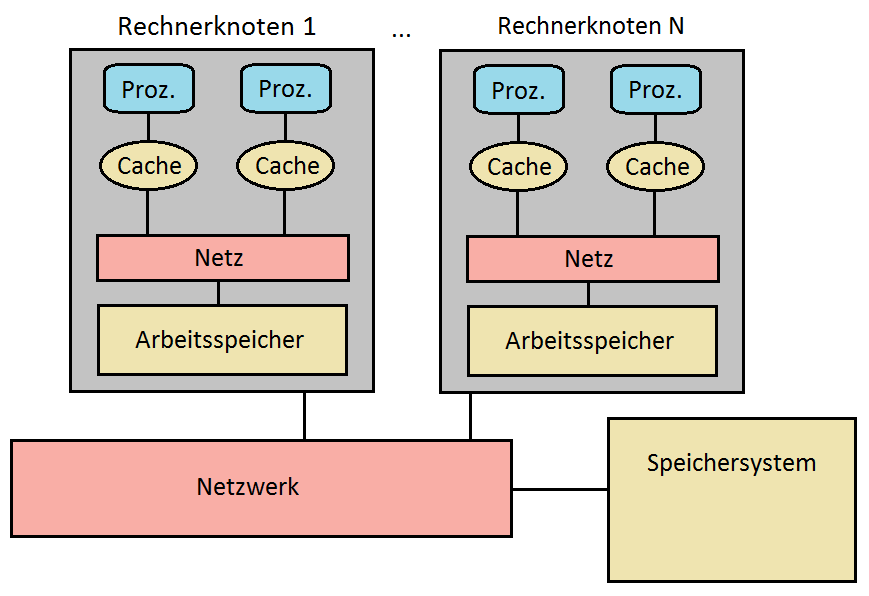
\includegraphics[width=.43\textwidth]{Bilder/rechnerknoten.png}
	\end{center}
	\caption{Struktur des Hochleistungsrechners}
	\label{fig:rechnerknoten}
\end{figure}

Notwendig wird Hochleistungsrechnen in der Forschung für die Simulation von numerischen Modellen aus verschiedensten Bereichen, beispielsweise für Mehrkörpersimulationen in der Astronomie, für Strömungssimulationen oder zur Berechnung von Klimaprognosen.
\medskip

Wichtige Themen im Hochleistungsrechnen sind die effiziente Ausnutzung der zur Verfügung stehenden Leistung, das Erkennen und Beheben von Fehlern des parallelisierten Programmcodes, die Bereitstellung der Rechen- und Speicherkapazitäten, sowie die Energieeffizienz von Hard- und Software.
Um einen Supercomputer gut ausnutzen zu können ist bei vielen Anwendungen eine leistungsfähige Ein-/Ausgabe von großer Wichtigkeit. Bedingt ist dies dadurch, dass die Menge der anfallenden Daten wesentlich stärker ansteigt, als die Geschwindigkeit der Verbindungen zwischen den verschiedenen Speichermedien und -orten.

Die in \ref{E/A} beschriebene Ein-/Ausgabe erweitert sich im Rechnerverbund zur parallelen E/A, dies bedeutet einerseits, dass eine Datei von mehreren Prozessen zeitgleich gelesen und bearbeitet werden kann, und andererseits, dass eine Datei über mehrere Festplatten und Netzwerk-Server verteilt sein kann. Diese Parallelität hat einen wesentlichen Einfluss auf die Aufgabe der E/A-Leistungsvorhersage, denn statt nur den Aufwand der Arbeitsschritte auf einer einzelnen Festplatte abzuschätzen, müssen hier die verstrickten Zusammenhänge zwischen Netzwerken von Festplatten und Rechnern, den jeweiligen Auslastungen der Komponenten, sowie Priorisierungen bestimmter Aufgaben und Instanzen durch die Speicherverwaltung.

Die Erfassung aller dieser Informationen wäre sehr aufwendig, sodass dies zur Zeit nicht möglich ist. Eine Vorhersage von E/A-Leistung eines parallelen Dateisystems ist daher sehr schwierig.

\section{Maschinelles Lernen}
\label{back_ML}
Maschinelles Lernen gehört zu den Themengebieten künstliche Intelligenz und automatisierte Wissensgenerierung. Verfahren dieser Disziplin versuchen durch intelligentes Lernen von Mustern Vorhersagen und Entscheidungen zu treffen.
Als intelligent wird ein maschinelles Verfahren bezeichnet, dass vorgegebene Informationen nicht auswendig lernt und wiedergibt, sondern von diesen Informationen abstrahiert.
Durch eine globale Sichtweise auf die Daten können Gesetzmäßigkeiten zwischen den Trainingsdaten erkennt werden.
Die Trainingsdaten sind die Informationen, die dem Algorithmus bekannt sind.
Ein Testdatensatz dagegen ist eine Menge von ungesehenen Daten mit denen die Ergebnisse des maschinellen Lernens verglichen werden können.
Ein Attribut ist eine messbare Größe der Objekte, die untersucht werden. Dies könnte beispielsweise bei einem Datensatz über Blumen die Farbe der Blütenblätter sein.
Ein Datenpunkt beschreibt ein spezifisches Objekt (z.B. ein bestimmtes Exemplar der Blume), dazu enthält er einen an der Instanz gemessenen Wert zu jedem Attribut.

Typische Aufgaben des maschinellen Lernens sind die Klassifizierung und Regressionsanalyse von Daten.
\begin{itemize}
\item Es muss zwischen Klassifizierung und Klassifikation unterschieden werden.
\begin{itemize}
\item Als Klassifikation bezeichnet man die Zuordnung eines Objekts mit spezifischen Attributen zu einer bestimmten Gruppe von Objekten mit ähnlichen Attributen.
\item Der zur Klassifikation genutzte Klassifikator ist das Ergebnis einer Klassifizierung.
Zur Klassifizierung können Verfahren des maschinellen Lernens genutzt werden. Bei der Klassifizierung muss von den eigentlichen Objekt-Attributen abstrahiert werden, sodass Muster zwischen den Objekten erkannt werden können. Dann können Klassengrenzen definiert werden, die jeder Klasse einen Bereich des Attribut-Raumes zuordnet. Ein Klassifikator muss die Werte der Attribute eines neuen Objekts, das noch keiner Klasse zugewiesen wurde, anschließend nur mit den Klassengrenzen vergleichen und findet so die passende Zuordnung.
\end{itemize}
\item Regressionsanalyse (oft auch nur Regression) ist ein Verfahren zur Bestimmung der Zusammenhänge von einem spezifischen Zielvariablen zu den übrigen Objekt-Attributen. Wenn in einem Datensatz die Einträge zur Zielvariablen fehlen, können die berechneten Relationen zur Prognose der unbekannten Werte mit Hilfe der bekannten Attribute genutzt werden. Die Zielvariable wird so über die Abhängigkeit zu anderen Variablen durch ein Verfahren des maschinellen Lernens modelliert. Das erhaltene Modell aus dem Verfahren wird auch als Prädiktor bezeichnet. 	
\end{itemize}

Ein Verfahren bzw. Algorithmus des maschinellen Lernens erstellt also ein Modell, welches einerseits Aussagen über die zur Verfügung stehenden Daten trifft und darüber hinaus Aussagen über unbekannte Variablen treffen kann.
Bei der Klassifikation wird eine qualitative Aussage über neue Datenpunkte anhand der Einordnung in Gruppen getroffen.
Beim Regressionsmodell wird dagegen eine quantitative Aussage über die Zusammenhänge zwischen den Attributen der Daten getroffen. Das Modell approximiert einen Wert für ein bestimmtes Attribut neuer Datenpunkte voraus, wenn außer der Zielvariablen alle Attribut-Werte gesetzt sind.  
Klassifizierung und Regression können weitergehend über ihr Lernverhalten unterschieden werden.
Während bei der Regression überwachtes Lernen stattfindet, wird bei der Klassifizierung unüberwacht gelernt. Der Unterschied der beiden Varianten befindet sich in den Informationen die im Trainingsdatensatz enthalten sind.
\begin{itemize}
\item Die Instanzen der Trainingsdaten beim überwachten Lernen enthalten auch die gesuchten Werte der Zielvariablen, dessen Werte der Algorithmus nach dem Lernvorgang auf dem Testdatensatz vorhersagen soll.
Für die Regressionsanalyse sind diese Informationen essentiell, da für die Modellierung die Zusammenhänge der Werte der Zielvariablen mit den restlichen Variablen untersucht werden muss.
Die Information über die idealen Ausgabewerte zur Zielvariablen werden während des Lernvorgangs genutzt um die Parameter des Prädiktors so anzupassen, sodass er die vorgegebenen Werte möglichst gut approximiert. Wichtig ist dabei, dass der Prädiktor nicht zu sehr auf die Trainingsdaten zugeschnitten wird, sondern die abstrakteren Relationen erkennt, sodass auch auf den ungesehenen Testdaten gut vorhersagen gemacht werden können.
\item beim unüberwachten Lernen wird kein bestimmtes Ergebnis erwartet, stattdessen muss der Algorithmus versuchen den Informationen inhärente Abhängigkeiten und Zusammenhänge zu erkennen.
Wenn die Klassenzuordnungen bereits in den Trainingsdaten bekannt wären, hätte das Klassifizierungs-Verfahren nicht viel zu tun. 
Der Klassifizierung steht daher während dem Lernprozess auch keine Rückmeldung über die Güte der gemachten Klassifikation zur Verfügung. 
\end{itemize}

Die vom Klassifikator erstellten Gruppierungen werden üblicherweise nicht bewertet, da die Qualität einer Sortierung nur im Kontext des gewünschten Nutzens der Klassen beurteilt werden kann.
Zunächst einmal ist jede eindeutige Klassifizierung legitim.

Der Prädiktor der Regressionsanalyse kann dagegen konkret bewertet werden. Dazu wird der Testdatensatz benötigt. Die zu bestimmenden Werte der Zielvariablen sind in den Testdaten bereits vorgegeben.
Diese Information wird bei der Durchführung des Tests vorenthalten. Durch den Vergleich zwischen tatsächlicher und vorhergesagter Lösung können Rückschlüsse auf die Qualität der Vorhersagen gezogen werden können. Dazu werden Metriken zur Bestimmung der Güte der Modellierung benötigt.
Zur Anwendung einer Regressionsanalyse müssen also zunächst Kriterien bzw. Leistungsmetriken eingeführt werden, anhand derer die Qualität der Vorhersagen und Entscheidungen gemessen werden können. Einerseits zum Vergleich der Vorhersagen auf den Testdatensatz zwischen verschiedenen Ansätze, aber auch bereits für den Lernprozess des Algorithmus selbst, damit dieser sozusagen aus seinen Fehlern und Erfolgen lernen kann. Eine einfache Metrik wäre beispielsweise die mittlere Modellabweichung der Vorhersagen gegenüber den \textit{Lösungswerten}.
\medskip

Oft ist es notwendig die zur Verfügung stehenden Daten aufzubereiten, bevor ein maschineller Lernalgorithmus effizient und korrekt Informationen aus diesen ableiten kann.
Nach Alpaydin können fehlerhafte Daten ein Problem sein, die durch zufälligen Messfehler oder eine systematisch inkorrekte Messung entstehen können \cite{Alpaydin:2010:IML:1734076} (S. 13-15). Zudem schreibt er, dass Teile der Daten überflüssig sein können, da sie redundant sind oder keine relevanten Informationen enthalten. Problematisch sind auch Datenpunkte mit gleichen Eingabewerten, aber unterschiedlichen Werten zur Zielvariablen \cite{Alpaydin:2010:IML:1734076} (S. 14).
Mit all diesen Problemen muss, unter Beachtung der Eigenschaften des vorliegenden Datensatzes, bei der Aufbereitung der Daten sinnvoll umgegangen werden. So können beispielsweise Ausreißer bei den Daten aussortiert werden, da diese eventuell durch eine Fehlmessung entstanden sind. Widersprüchliche Datenpunkte können zusammengefasst werden, indem sie zusammen einen neuen Datenpunkt mit eindeutigen Ausgabewerten bilden (dies könnten die Mittelwerte sein).

\subsection{Clusteranalyse}
Eine typische Anwendung der Klassifizierung ist die Clusteranalyse.
Kantardzic beschreibt Clusteranalyse folgendermaßen: \glqq Cluster analysis is the formal study of methods and algorithms for natural grouping, or clustering, of objects according to measured or perceived intrinsic characteristics or similarities.\grqq{} \cite{kantardzic2011data} (S. 250). Ein einfaches und anschauliches Beispiel sind Punkte im zweidimensionalen Raum, die hinsichtlich ihrer Position gruppiert werden (siehe Abbildung \ref{fig:clustering_beispiel}).

\begin{figure} [h]
	\subfloat{
		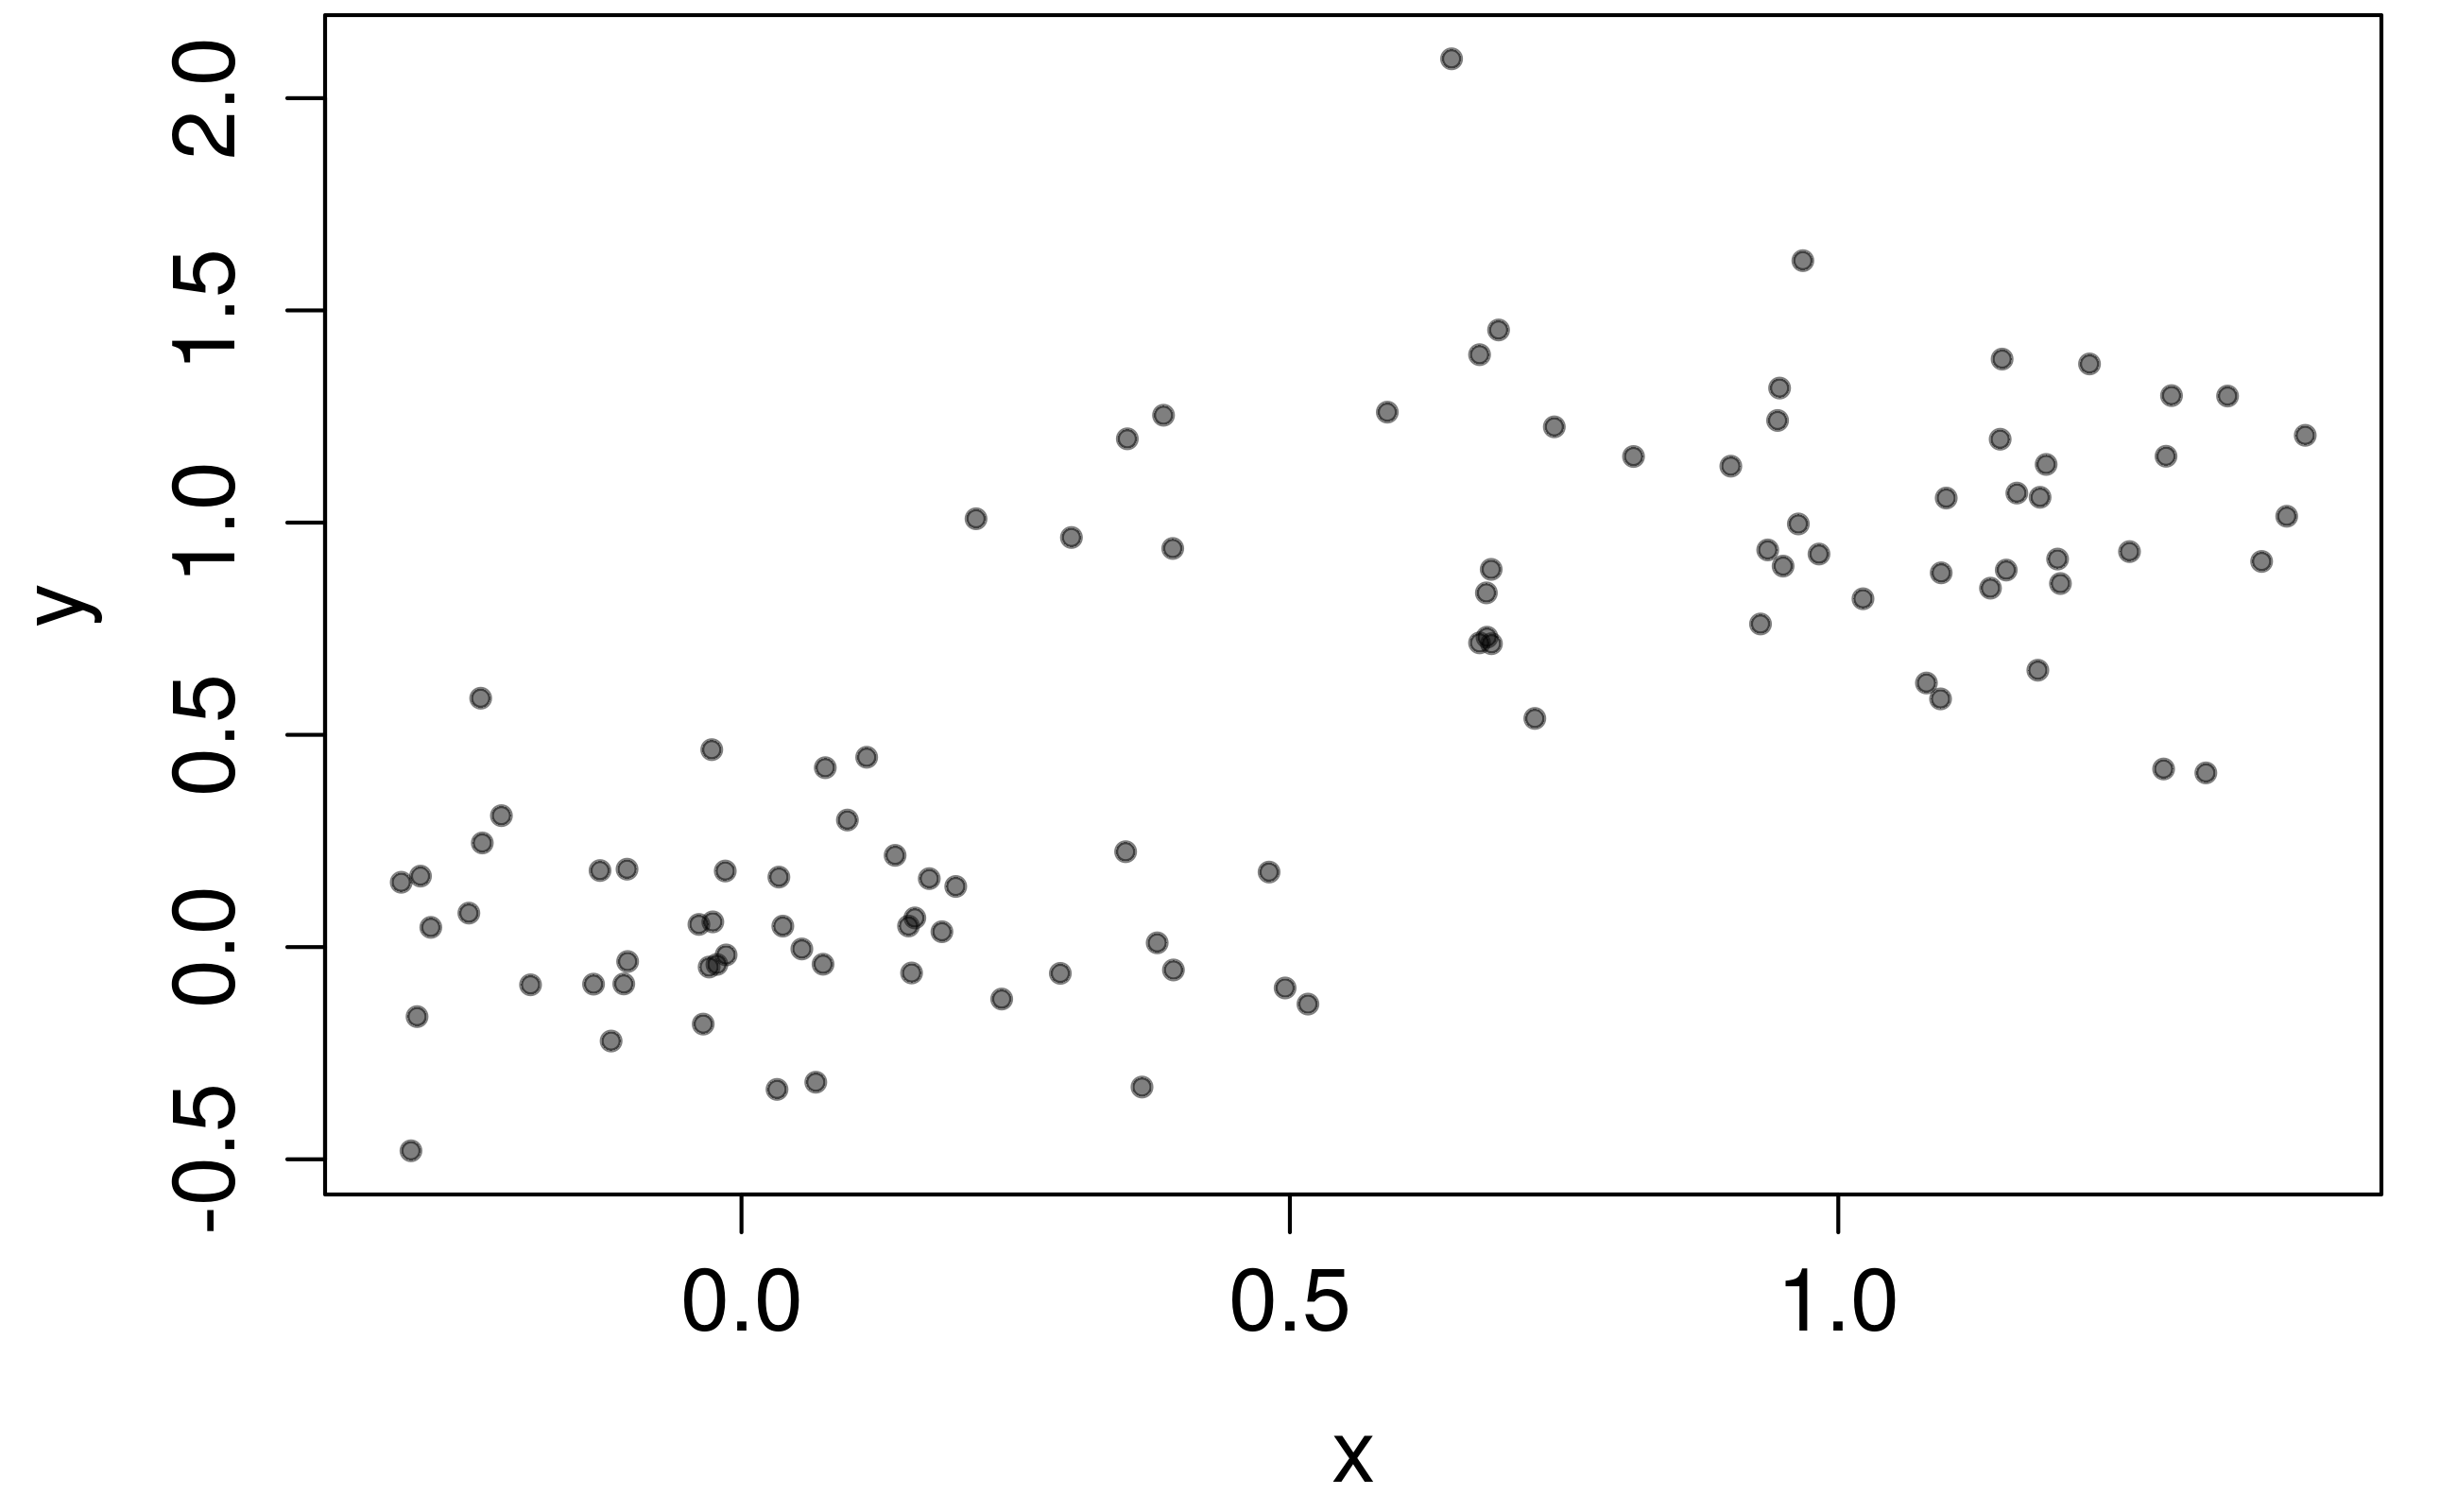
\includegraphics[width=.5\textwidth]{Bilder/test_clustering_points.png}
	}
	\hfill
	\subfloat{
		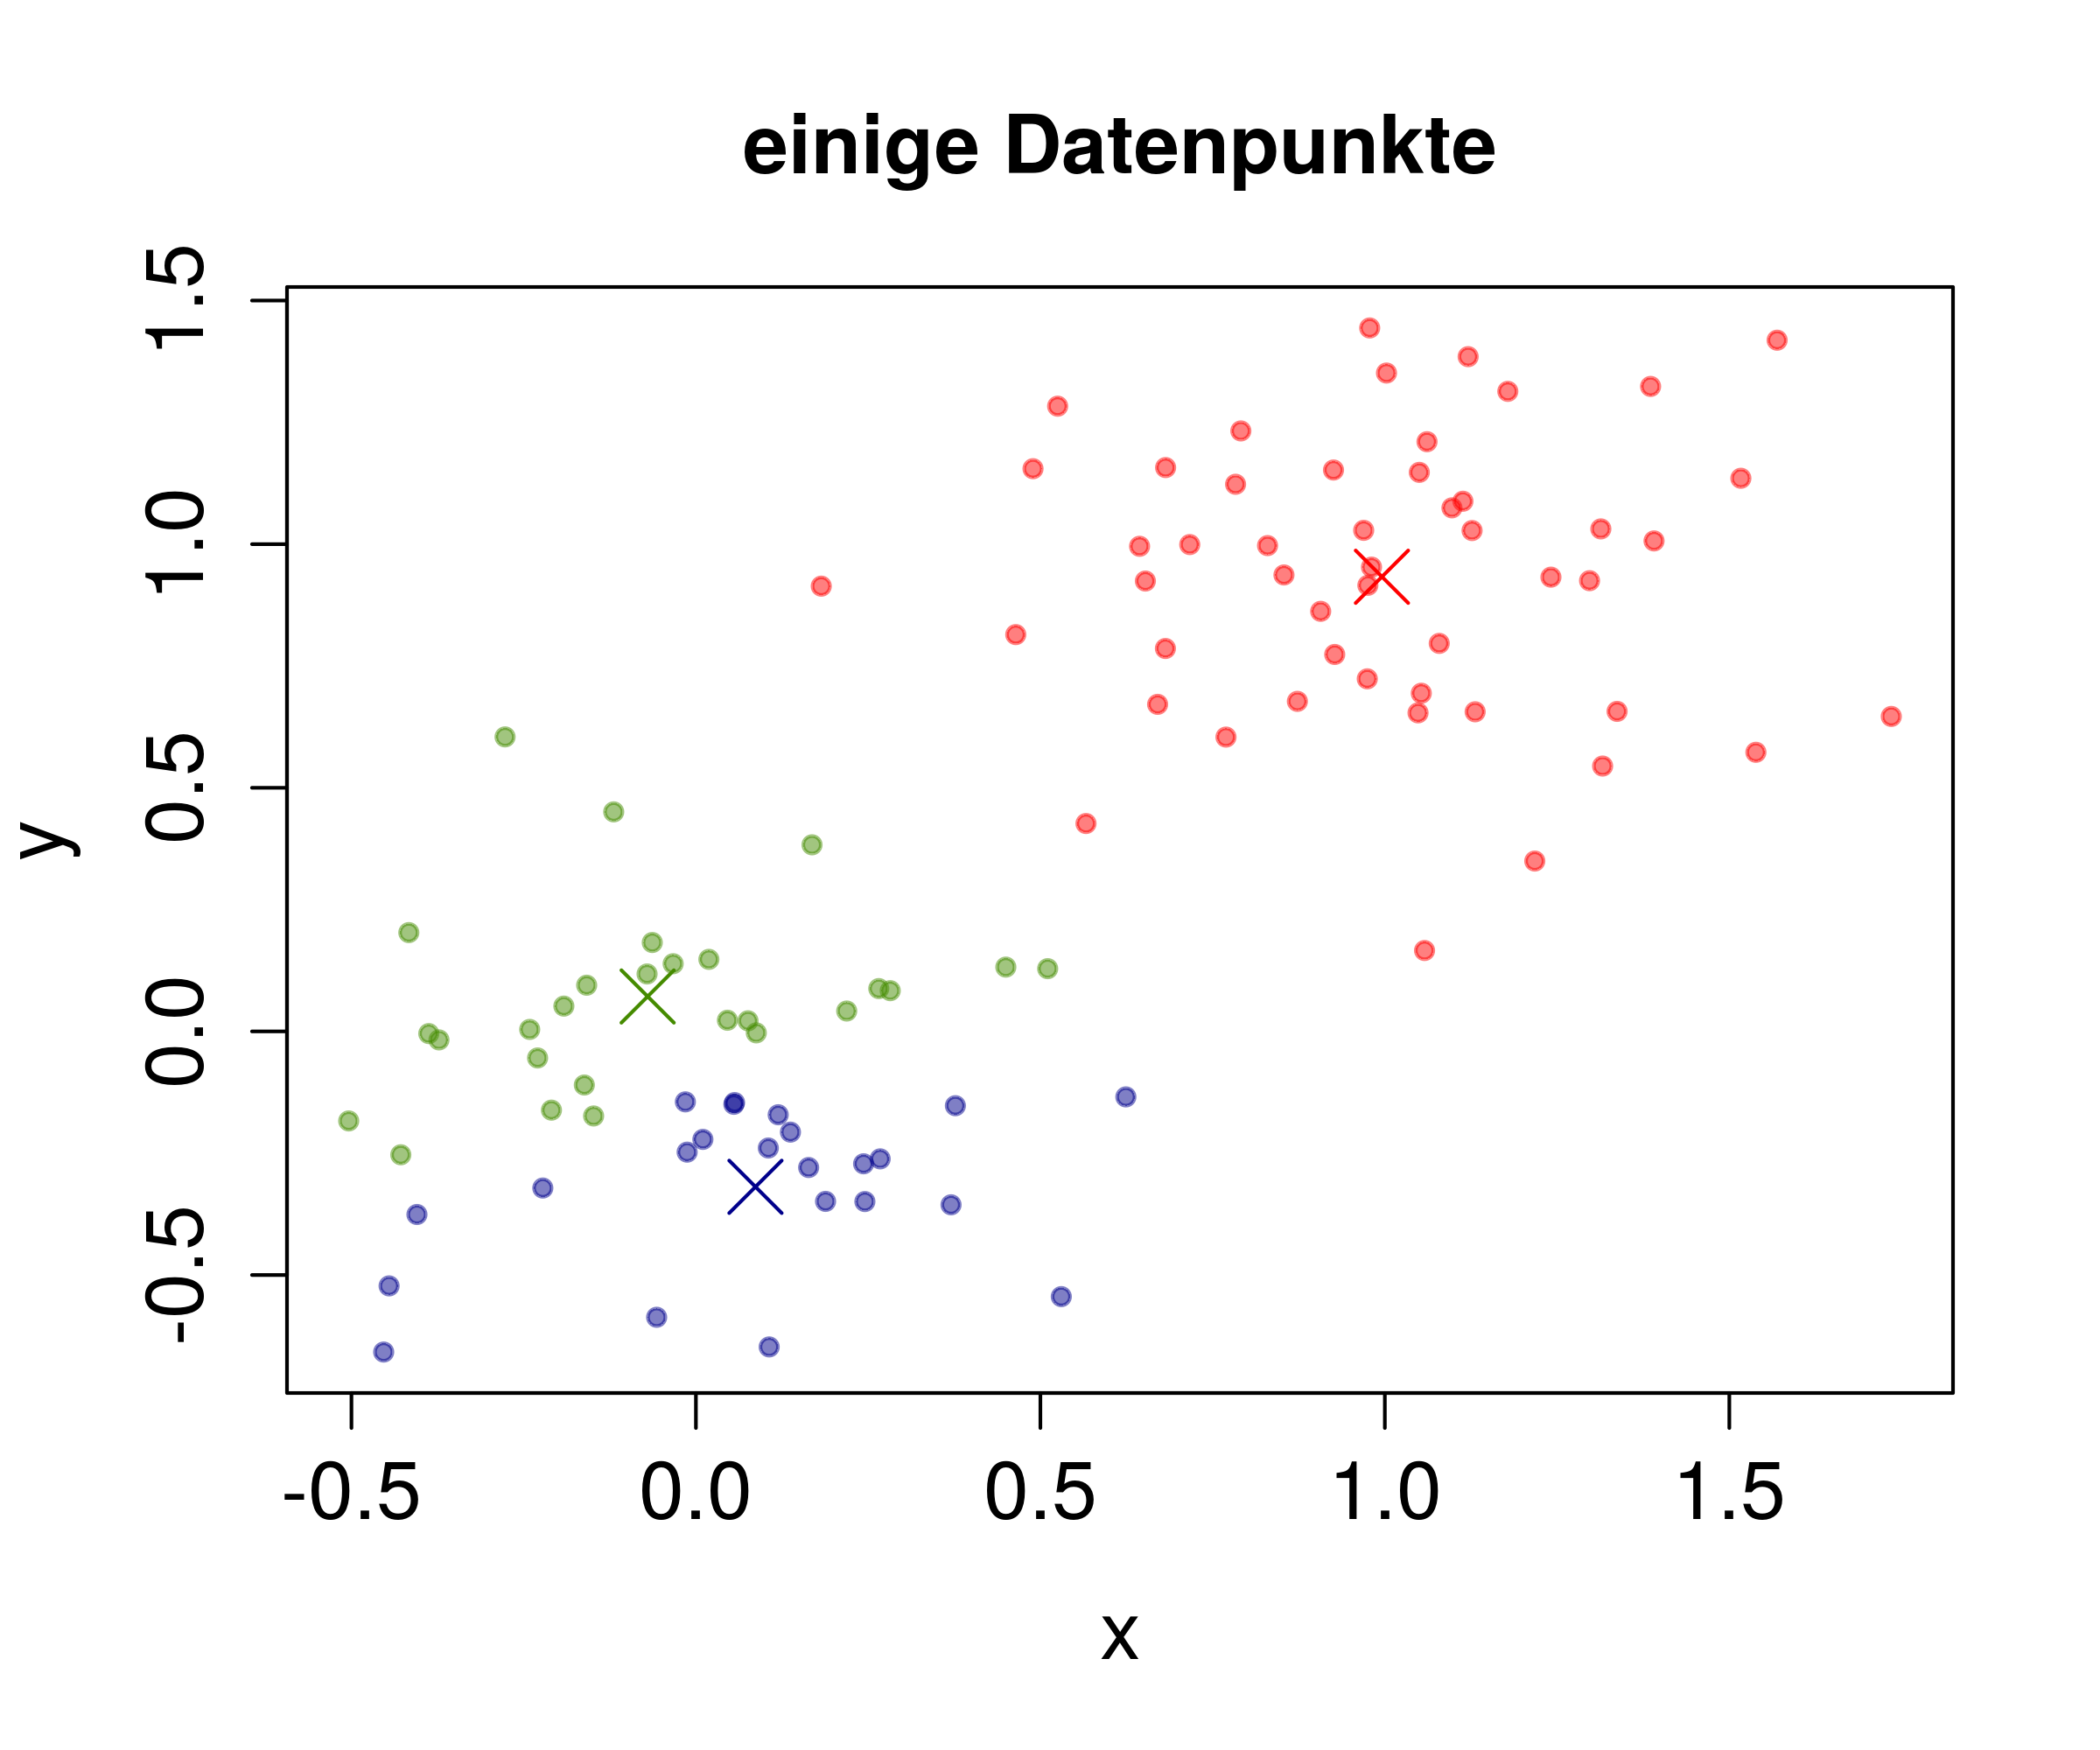
\includegraphics[width=.5\textwidth]{Bilder/test_clustering.png}
	}	
	\caption{Datenpunkte mit je einem Wert für x und y-Dimension. Rechts farbliche Markierung für die Zugehörigkeit zu den drei vom k-Means-Algorithmus bestimmten Clusters. Ein Kreuz markiert den Mittelpunkt des Clusters (Mittelwert aller zugehörigen Punkte)}
	\label{fig:clustering_beispiel}
\end{figure} 

Ein einfacher Clustering-Algorithmus ist der k-Means-Algorithmus. Bei diesem muss zunächst die Anzahl Cluster $k$ festgelegt werden. Die $k$ Mittelwerte der Cluster werden mit zufälligen Werten initialisiert. Dann wird jeder Datenpunkt dem Cluster zugeordnet, dessen Mittelwert seinem am dichtesten ist. Danach werden die Mittelwerte der Cluster anhand der Ihnen zugeordneten Punkte berechnet und gesetzt. Das Neuzuordnen der Punkte und Berechnen der Mittelwerte wird nun solange wiederholt, bis sich keine Änderung der Zuordnung mehr ergibt. Als Endergebnis eines Cluster-Algorithmus erhält man eine Gruppierung der Datenpunkte in Mengen mit möglichst niedriger Varianz innerhalb eines Clusters und möglichst großer Varianz zwischen den Clustern.

\section{Künstliche Neuronale Netze}
\label{back_nn}
Bei künstlichen neuronalen Netzen, im Folgenden nur neuronale Netze genannt, handelt es sich um eine Methode aus dem Bereich des maschinellen Lernens zum Approximieren einer unbekannten Funktion, die der Relation zwischen zwei Datenmengen zugrunde liegt. Die Methode ist inspiriert von biologischen neuronalen Netzen, wie sie im Gehirn vorkommen. 
Sie verwenden einen statistischen Ansatz, ihre Lösung für das Problem wird zunächst zufällig im Lösungsraum angelegt und dann mit Hilfe eines Gradientenverfahrens optimiert.
Rojas \cite{Rojas:1996:NNS:235222} vergleicht neuronale Netze mit einer Black Box, also einem System mit beobachtbarer Ein- und Ausgabe, aber unbekannter innerer Verarbeitung der Informationen. 
Zur Verwendung eines neuronalen Netzes gibt man dem Netz eine Menge von Eingabevektoren $E \in \mathbb{R}^n$ mit jeweils zugehörigem Ausgabevektor $A \in \mathbb{R}^m$ vor und dieses versucht eine passende Funktion $F: \mathbb{R}^n \rightarrow \mathbb{R}^m$ zu finden. Dementsprechend handelt es sich hierbei um überwachtes Lernen, da eine gewünschte ideale Ausgabe vorgegeben wird.

\begin{figure}[h]
	\begin{center}
		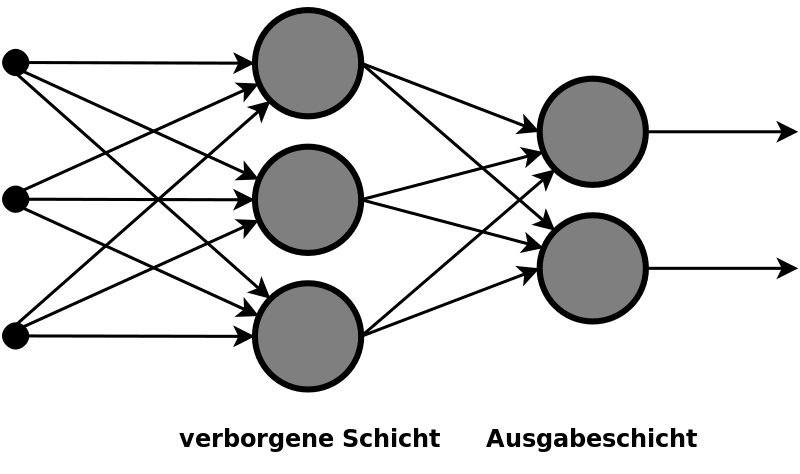
\includegraphics[totalheight=0.2\textheight]{Bilder/Multi-Layer_Neural_Network-Vector.png}
	\end{center}
	\caption{Zweischichtiges Netz Quelle: Offnfopt, \url{https://de.wikipedia.org/w/index.php?title=Datei:Multi-Layer_Neural_Network-Vector.svg&lang=de}}
	%
	\label{fig:Schichten}
\end{figure}

Ein feedforward-Netz besteht aus einer Eingabeschicht, einer beliebigen Anzahl verborgener Schichten und einer Ausgabeschicht (siehe Abbildung \ref{fig:Schichten}), wobei die Verbindungen aus jeder Schicht jeweils nur in die Nächsthöhere gehen. 
Die Eingabeschicht besteht, meiner vorherigen Definition entsprechend, aus $n$ Stellen, an denen die Werte eines Eingabevektors stehen. Jeder Eingabewert wird dann an jedes Neuron in der ersten verborgenen Schicht weitergegeben und dort verrechnet, die Ergebnisse der Neuronen der verborgenen Schicht werden dann an die nächste Schicht gegeben und so weiter.
Die Ergebnisse der Ausgabeschicht bilden den Ausgabevektor mit Länge $m$.
Rekurrente Netze haben die gleiche Struktur, doch es können auch Verbindungen zu zurückliegenden Schichten vorkommen, dadurch ist die Berechnung zu einem Eingabevektor nicht mehr deterministisch bestimmt. Es müssen Berechnungs- und Determinierungsregeln festgelegt werden. 

\begin{figure}[h]
	\begin{center}
		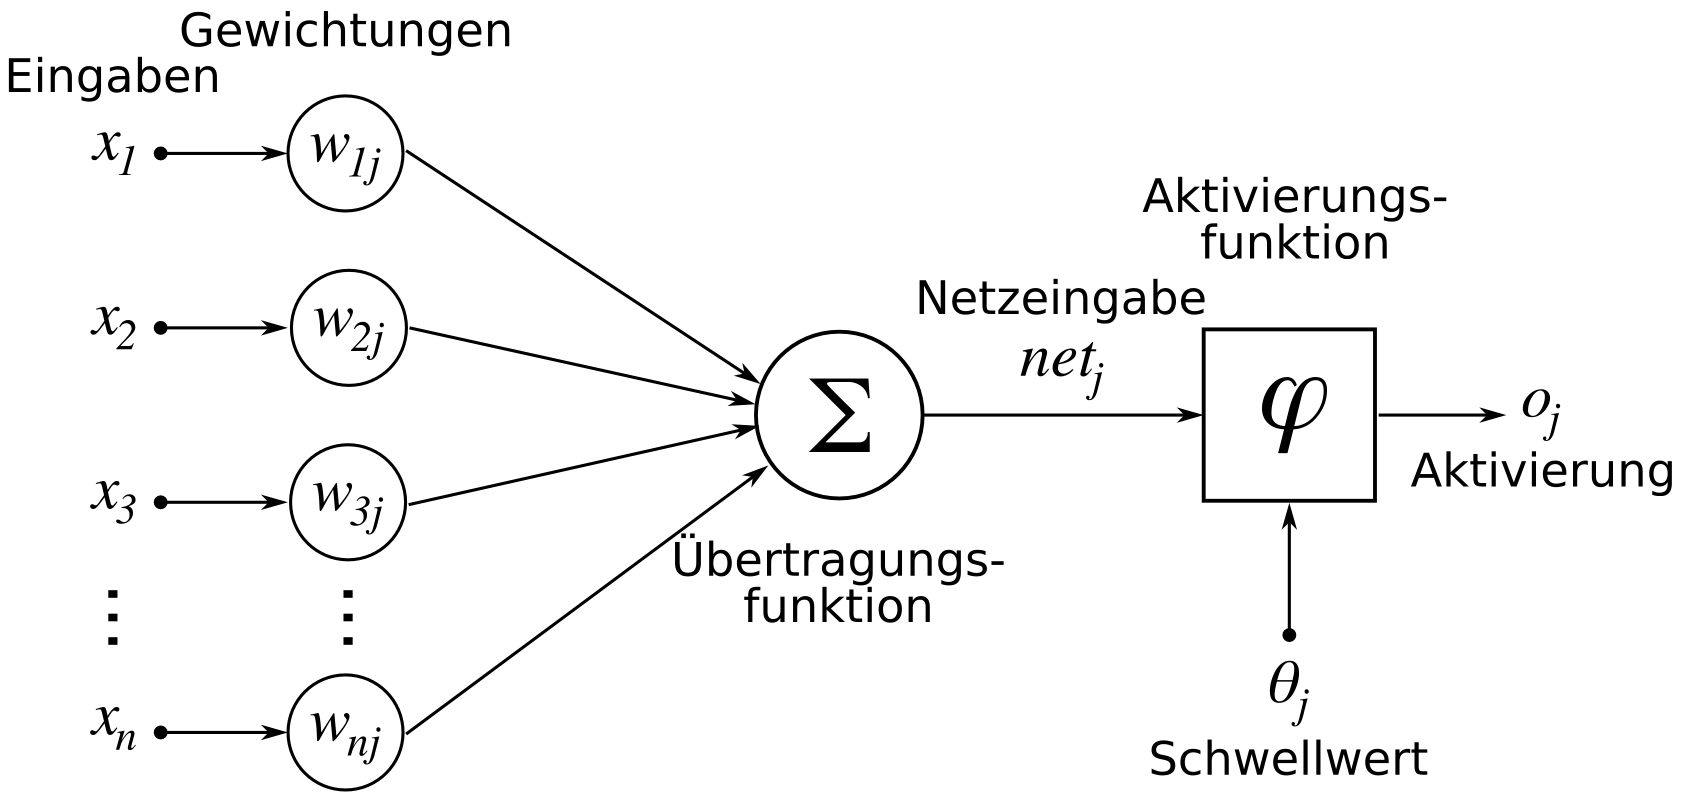
\includegraphics[totalheight=0.2\textheight]{Bilder/ArtificialNeuronModel_deutsch.png}
	\end{center}
	\caption{Schema eines künstlichen Neurons. Quelle: Chrislb, \url{https://de.wikipedia.org/wiki/Datei:ArtificialNeuronModel_deutsch.png}} %
	\label{fig:Neuron}
\end{figure}

Jedes Neuron rechnet die eingehenden Eingabewerte mit einer zur Übertragungskante zugehörigen Gewichtung mit einer Übertragungsfunktion zusammen, die Anzahl der Eingaben ist hierbei unbegrenzt (\glqq unlimited fan-in property\grqq{} \cite{Rojas:1996:NNS:235222}). Die Übertragungsfunktion kann hierbei schlicht die Summe aller gewichteten Eingaben sein. Der errechnete Wert wird als Netzeingabe an die Aktivierungsfunktion gegeben. 
Die Aktivierungsfunktion berechnet eventuell mit oder ohne einem Schwellwert die Aktivierung des Neurons, welche dann an alle verbundenen Neuronen der nächsten Schicht weitergegeben wird.
Die Aktivierungsfunktion kann beispielsweise eine simple Stufenfunktion sein, die allen Netzeingaben kleiner des Schwellwerts eine Null und allen Eingaben größer gleich des Schwellwerts eine Eins zuweist.

Ein Neuron mit der gewichteten Summe aller Eingaben als Übertragungsfunktion und einer Stufenfunktion mit Schwellwert als Aktivierungsfunktion wird von Rojas \textit{Perzeptron} bezeichnet \cite{Rojas:1996:NNS:235222} (S. 60).
\medskip

Ein feedforward-Netzwerk aus Perzeptrons, in dem jedes Neuron mit allen Neuronen der folgenden Schicht verbunden ist, wird als \textit{multilayer perceptron} (kurz MLP) bezeichnet.
Ein neuronales Netz lernt die Abbildung zwischen den vorgegebenen Paaren von Eingabe- und Ausgabedaten durch Anpassung der Gewichte an den Kanten, nachdem es mit zufälligen Kantengewichten initialisiert wurde.
Diese Anpassung geschieht beim MLP durch Fehlerrückführung (engl. backpropagation). Dabei wird der mittlere quadratische Fehler der berechneten Ausgabe gegenüber der vorgegebenen Ausgabe ermittelt und daraufhin unter Rücksichtnahme auf eine Lernrate mit Hilfe des Gradientenverfahren minimiert.

\subsection{Berechenbarkeitstheorie neuronaler Netze}
Vor der Anwendung von künstlichen neuronalen Netzen für ein Problem stellt sich die Frage, ob diese für das Problem geeignet sind. Dazu gibt es einige interessante mathematische Beweise.
Ein einzelnes Perzeptron kann alle linear separierbaren logischen Funktionen exakt approximieren \cite{Rojas:1996:NNS:235222} (S. 62-63). 
Wobei lineare Separierbarkeit nach Rojas definiert ist als:

Zwei Punktmengen A und B in einem n-dimensionalen Raum sind linear separierbar, wenn $n + 1$ reelle Zahlen $w_1,...,w_{n+1}$ existieren, sodass für jeden Punkt $(x_1,x_2,...,x_n) \in A$ die Ungleichung $\sum_{i=1}^{n} w_ix_i \ge w_{n+1}$ gilt und für jeden Punkt $(x_1,x_2,...,x_n) \in B$ $\sum_{i=1}^{n} w_ix_i < w_{n+1}$

\begin{figure}
	\subfloat[Zwei voneinander nicht linear separierbare Relationen in $ \mathbb{R}^2$.]{
		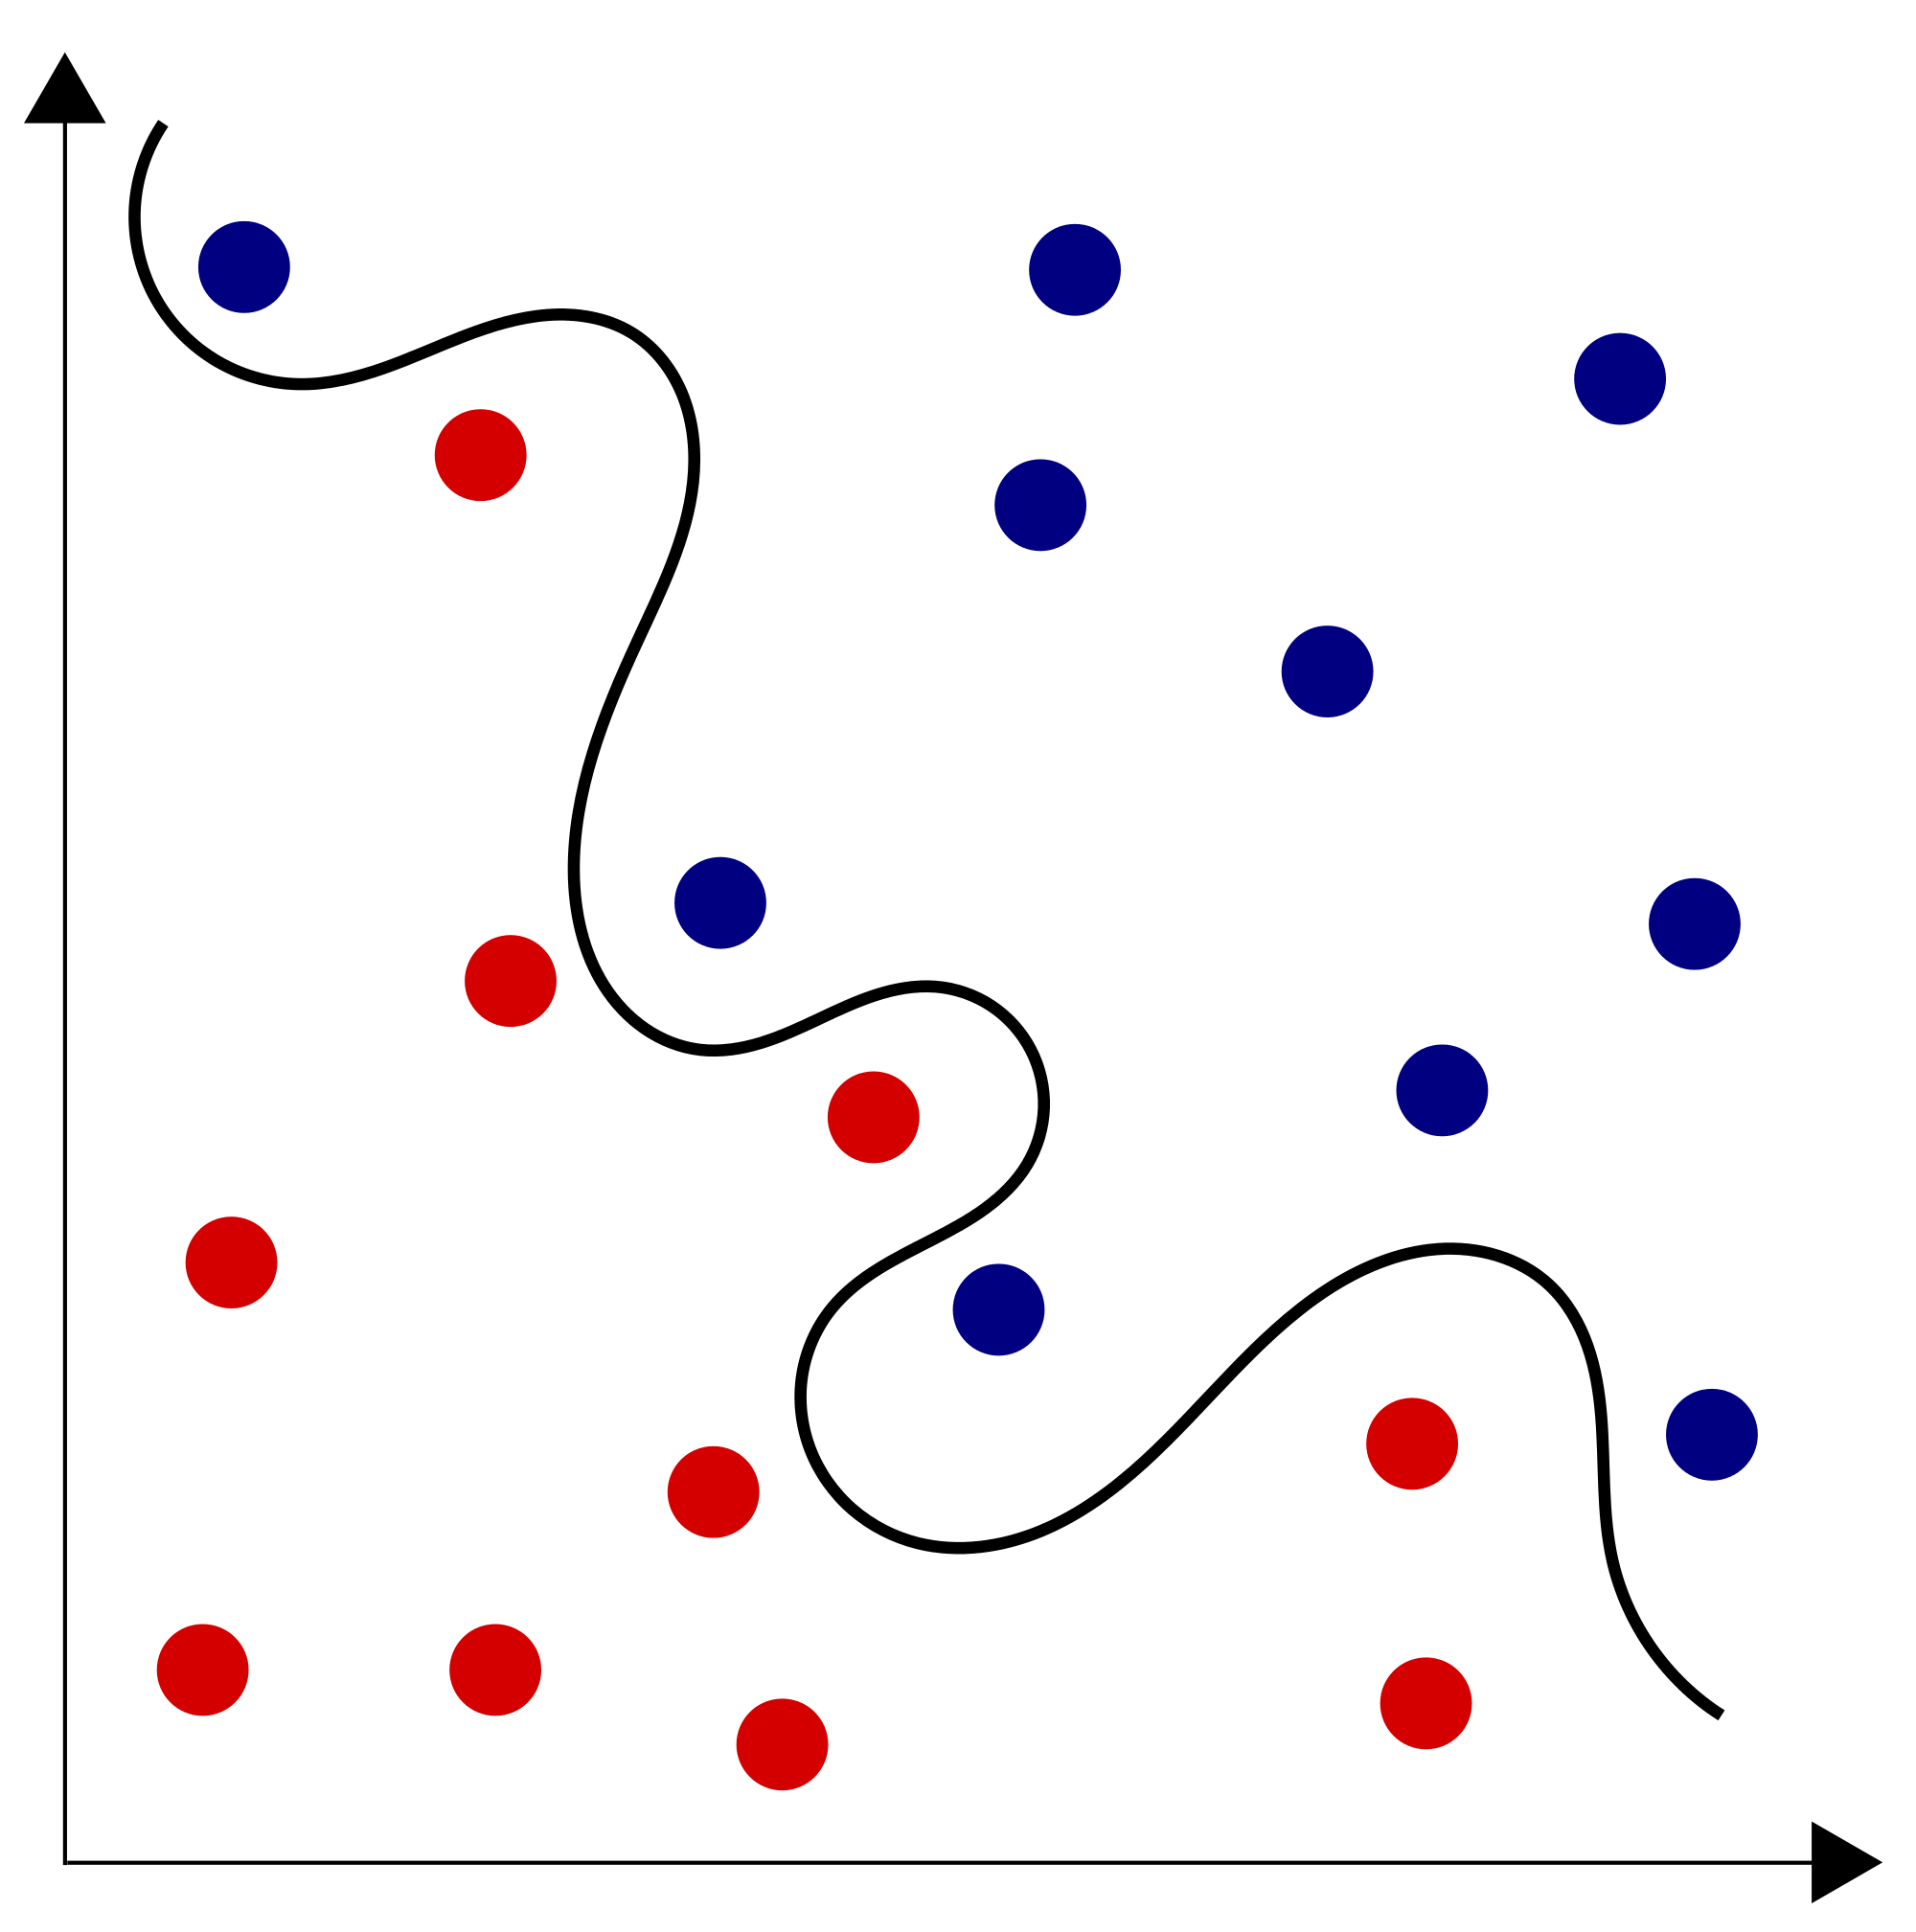
\includegraphics[width=.3\textwidth]{Bilder/2000px-Separability_NO.png}
	}
	\hfill
	\subfloat[Zwei voneinander linear separierbare Relationen in $\mathbb{R}^2$.]{
		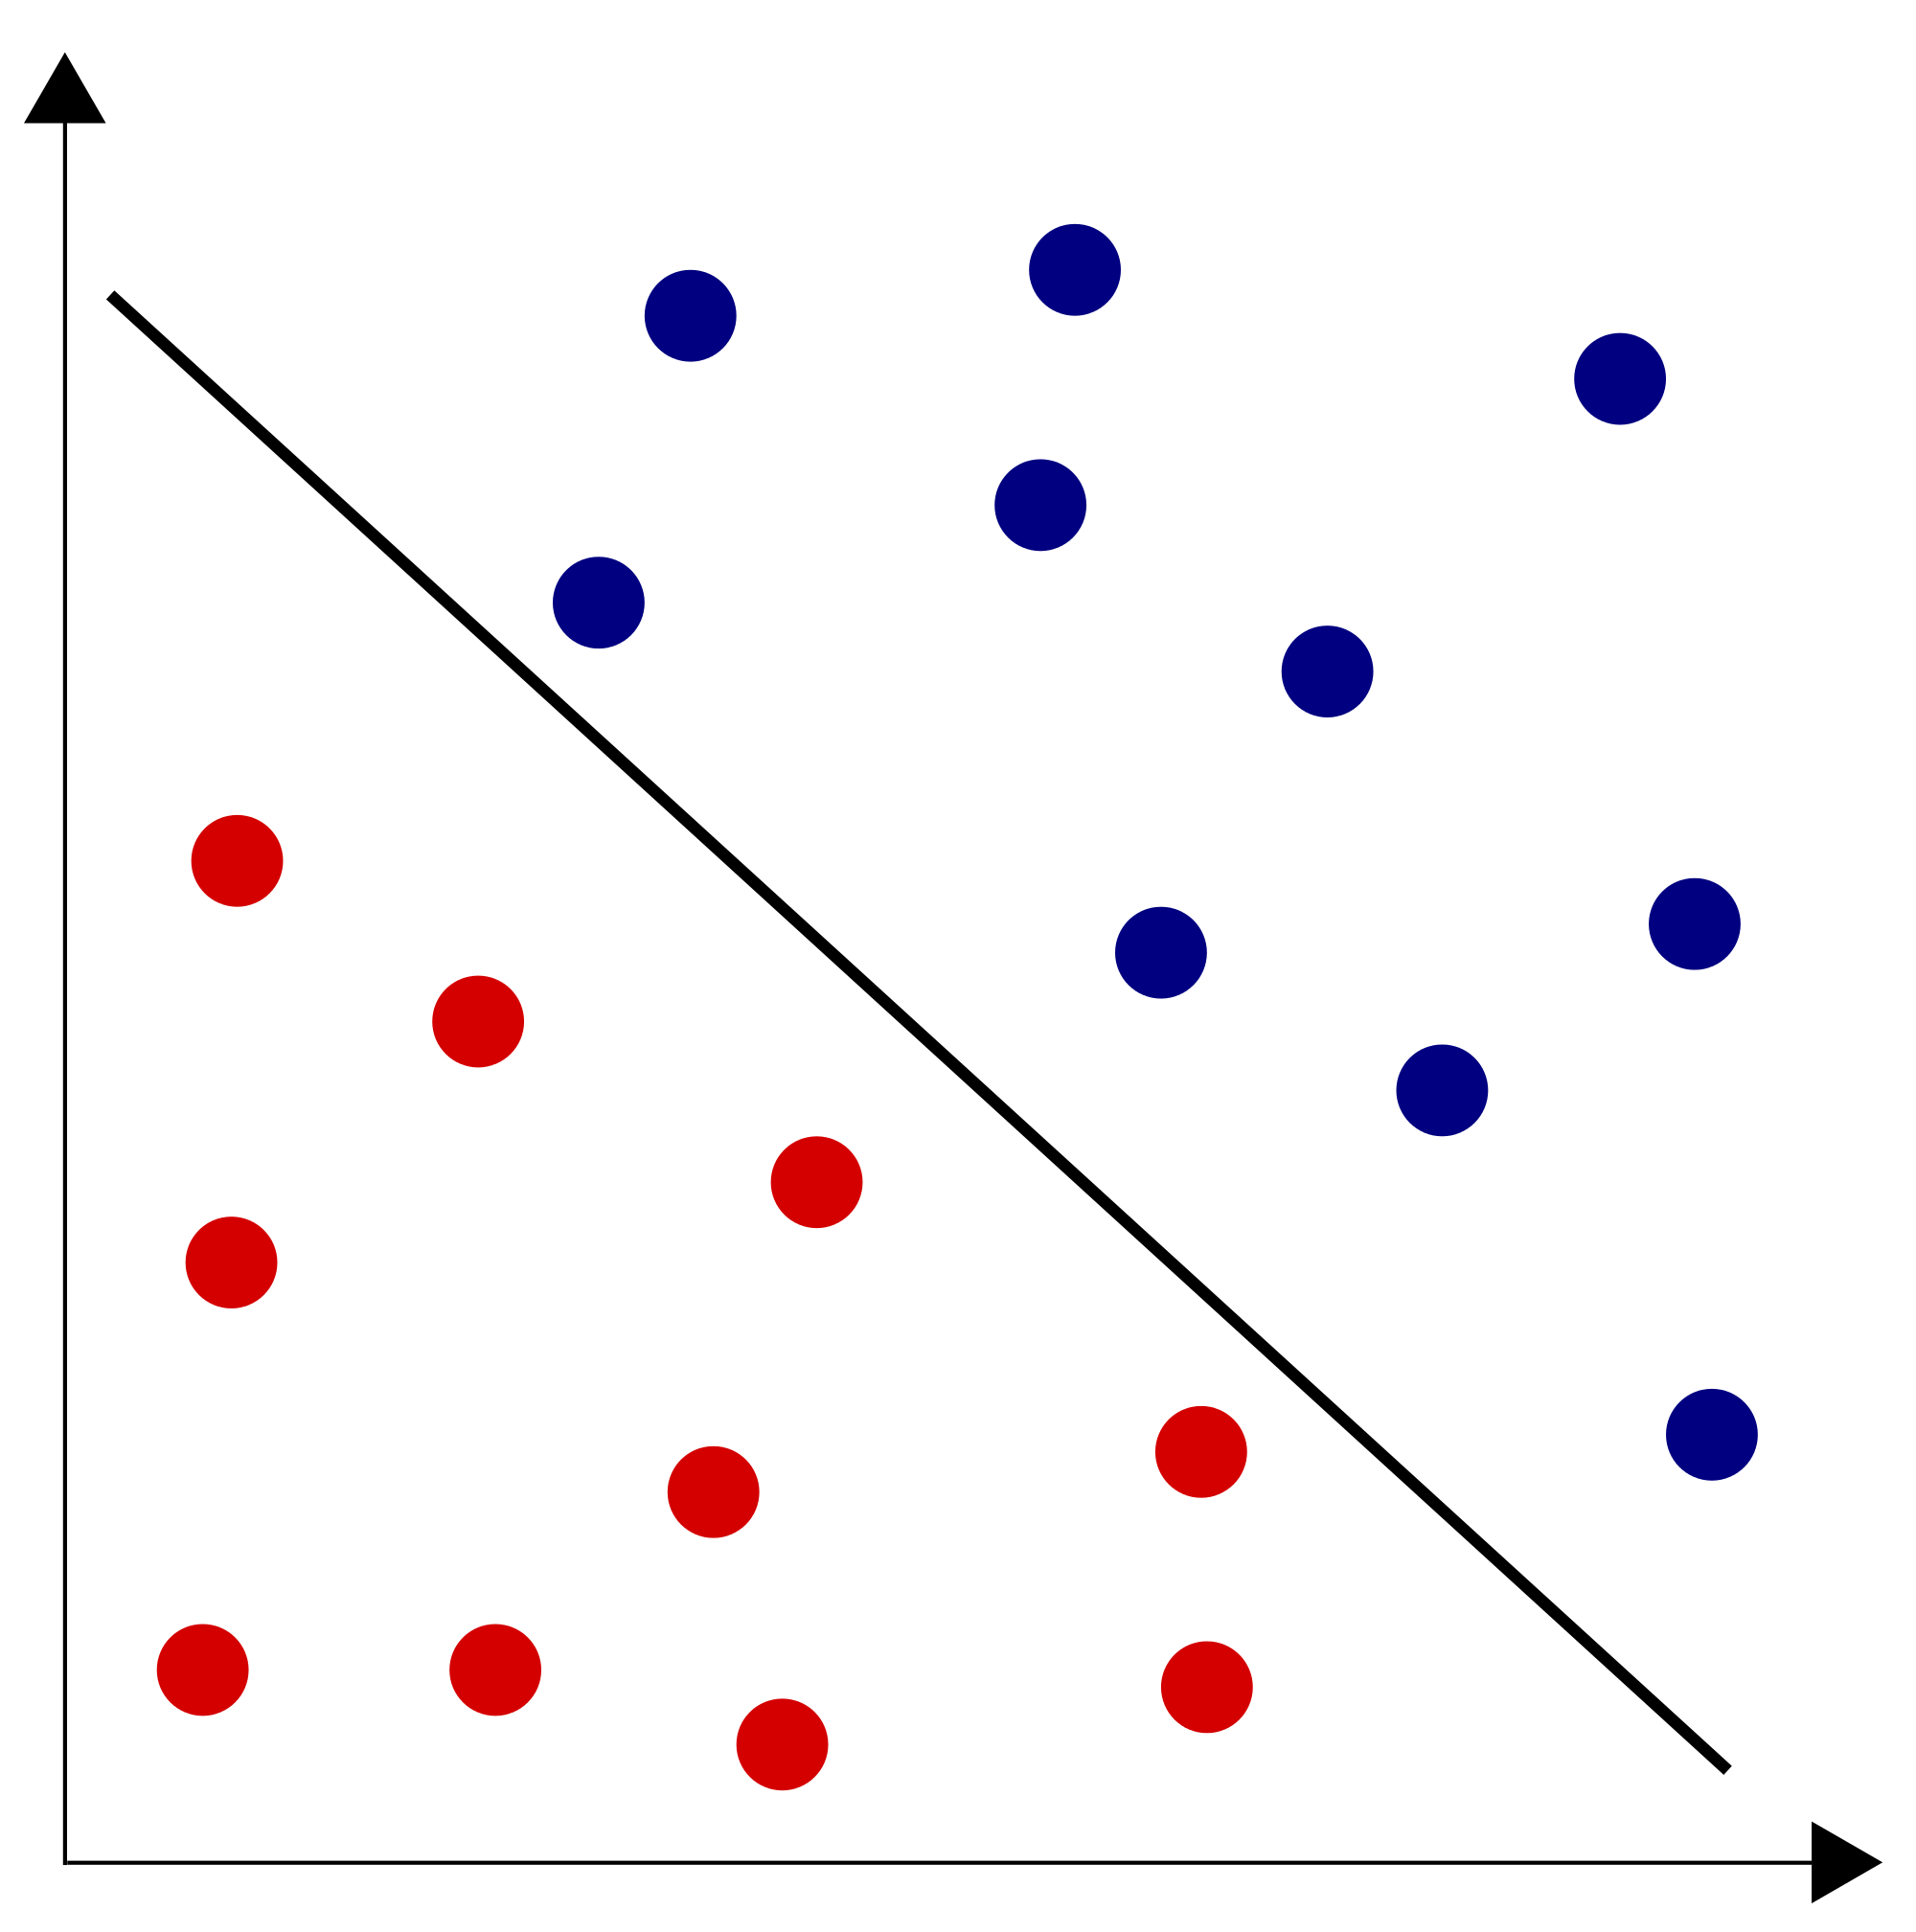
\includegraphics[width=.3\textwidth]{Bilder/2000px-Separability_YES.png}
	}		
	\caption{Lineare Separierbarkeit, Quelle: Mekeor, \url{https://de.wikipedia.org/wiki/Datei:Separability_YES.svg} und \url{https://de.wikipedia.org/wiki/Datei:Separability_NO.svg}}
	%
	\label{fig:separierbarkeit}
\end{figure} 

Diese Beschränkung gilt allerdings nicht für ein Netzwerk von Neuronen. Bereits ein zweilagiges Netzwerk aus noch simpleren McCulloch-Pitts-Zellen kann jede beliebige logische Funktion berechnen \cite{Rojas:1996:NNS:235222} (S. 37).
Für MLPs hat Cybenko \cite{cybenko:mcss} bewiesen, dass sie beliebige kontinuierliche Funktionen auf einer kompakten Teilmenge des euklidischen Raums $\mathbb{R}^n$ approximieren kann. Der entsprechende Satz hierzu ist das \textit{universal approximation theorem}.

\bigskip
\paragraph{Zusammenfassung:}
\textit{ 
	Das Kapitel hat einen kurzen Abriss der für diese Thesis relevanten Themen geliefert. Es wurde festgestellt, dass die Vorhersage von E/A-Laufzeiten im Hochleistungsrechnen eine komplexe Aufgabe ist. Zusätzlich zu dem ohnehin aufwendigen E/A-System eines normalen Rechners müssen die Komplikationen durch die Vernetzung des Hochleistungsrechners in Betracht gezogen werden.\\
	Das Problem der E/A-Leistungsvorhersage kann mit Hilfe maschinellen Lernens gelöst werden. Die Aufgabe entspricht dabei einer Regressionsanalyse. Durch Vorgabe gemessener Zugriffszeiten von E/A-Aufrufen kann überwachtes Lernen betrieben werden. Dabei werden die Abhängigkeiten zwischen Aufrufparametern und Zugriffszeit ausgenutzt um die unbekannten Laufzeiten unbekannter Zugriffe vorherzusagen.
	Solange die E/A-Leistung durch eine kontinuierliche Funktion beschrieben werden kann und alle dafür benötigten Informationen zur Verfügung stehen, kann ein künstliches neuronales Netz das Problem lösen.
}

\chapter{Verwandte Arbeiten}
\textit{%
	In diesem Kapitel werden wissenschaftliche Veröffentlichungen vorgestellt, die dieser Arbeit gegenüber relevante Themen behandeln. Es werden drei Teilgebiete des Problems der Leistungsvorhersage von E/A-Aufrufen im Hochleistungsrechnen behandelt.\\
	Als Erstes gehe ich in Abschnitt \ref{rel_ea-vorhersage} auf einige Arbeiten ein, die allgemeine E/A-Leistungsvorhersage behandeln. Dabei führe ich zunächst zwei Begriffe für Kategorien von Lösungsansätzen ein. Danach gehe ich in Unterkapitel \ref{rel_vorhersage-mit-nn} auf Arbeiten ein, sich mit der Verwendung von neuronalen Netzen zur Leistungsvorhersage beschäftigen.
	Und in Abschnitt \ref{rel_vorhersage_im-hpc} werden Veröffentlichungen diskutiert die Leistungsmodellierung speziell im Hochleistungsrechnen behandeln.
}
\bigskip

\section{Leistungsvorhersage von Ein-/Ausgabe}
\label{rel_ea-vorhersage}
Das Problem, die Zugriffszeiten auf Festplatten vorherzusagen, kann im wesentlichen durch zwei verschiedene Ansätze gelöst werden \cite{Crume:2013:FML:2538542.2538561} (S. 45).
\begin{itemize}
\item  Zum einen kann man versuchen das Festplattensystem in einem Modell nachzubilden, indem Hardwaredetails, wie die Rotationsgeschwindigkeit der Platte, die Reaktionszeit und Geschwindigkeit des Lesekopfs, sowie das Zusammenspiel der Komponenten bekannt sind oder entsprechende Parameter durch gezielte Untersuchung approximiert werden. Mit diesem möglichst exakten Modell können dann Zugriffe simuliert und die Laufzeit des Modells gemessen werden. Diese Messung kann daraufhin als Vorhersage für das reale System verwendet werden. Eine White-Box ist ein System dessen innere Funktionsweise bekannt ist. Modelle dieses Ansatzes können entsprechend als White-Box-Modelle bezeichnet werden.
\item Beim zweiten Ansatz wird vom eigentlichen Festplattensystem abstrahiert und stattdessen ein mathematisches Modell gesucht, das das Verhalten des Systems möglichst genau beschreibt.
Zur Entwicklung des mathematischen Modells wird eine Regressionsanalyse durchgeführt, dabei werden gemessene Leistungswerte von Festplattenzugriffen untersucht, um daraus passende Parameter für das Modell abzuleiten. Analog zur vorherigen Namensgebung kann dieser Ansatz als Black-Box-Modellierung bezeichnet werden, da hier ohne Wissen über die inneren Zustände des Systems modelliert wird.
\end{itemize}
Ich unterscheide daher im Folgenden zwischen dem White-Box-Modellierung, bei dem versucht wird das Festplattensystem nachzubilden (in der englischen Fachliteratur auch als \textit{analytic device modeling} und \textit{simulation modeling} bezeichnet) und der Black-Box-Modellierung, bei dem ein mathematisches Modell entwickelt wird.

\subsection{White-Box-Modellierung gegenüber Black-Box-Modellierung}
Die Nachteile von Modellen der White-Box-Modellierung liegen insbesondere darin, dass sie aufwendig zu konfigurieren sind. Beispielsweise schreiben Crume et al.:\glqq In fact, one of us (Oldfield) spent several months configuring DiskSim to model an existing device\grqq{} \cite{Crume:2013:FML:2538542.2538561} (S.45) und naturgemäß schnell veraltern, da sie jeweils an spezielle Hardware angepasst sind. Der Vorteil dagegen ist, dass sie bei korrekter Konfiguration sehr präzise sind. Ruemmler und Wilkes erzielten mit einem gut kallibrierten White-Box-Modell gute geringe Residuen bei der Vorhersage von Festplatten-Zugriffszeiten \cite{Ruemmler94anintroduction}. Um das Problem des hohen Aufwandts der exakten Parametriesierung für jedes Festplattenmodell anzugehen, haben sie untersucht, wie sich die Berücksichtigung verschiedener Festplattenkomponenten bzw. -eigenschaften auf den Modellfehler auswirkt. Sodass beim Einsatz des Modells Aufwand der Parametriesierung und Präzezion der Modellierung gegeneinander abgewägt werden können.

Eine weitere Arbeit, in der White-Box-Modellierung genutzt wurde stammt von Lebrecht et al. \cite{Lebrecht:2009:10.1109/QEST.2009.31}. Darin wird besonders auf ein Verfahren eingegangen, das dafür sogt, dass E/A-Anfragen in einer Reihenfolge abgearbeitet werden, die die notwendigen Bewegungen des Lese-/Schreibkopf möglichst gering hält.
\medskip

Die Black-Box-Modellierung ist in der Anwendung einfacher und flexibler, da es sich automatisch an das System anpasst. Dafür erwartet man aufgrund der fehlenden analytischen Einsicht ins System ungenauere Prognosen. Für die Anwendung im HPC-Bereich spielt der analytische Ansatz eine untergeordnete Rolle, da hier unterschiedliche Festplattensysteme zusammenarbeiten und stark mit der Netzwerkarchitektur verstrickt sind, sodass eine entsprechende Analyse des Systems aufwendig wird. \glqq Furthermore, the technical trend towards storage consolidation in large data centers hints that building an accurate model or simulator using white box method cannot be a genereal solution in serving a variety of very different workloads\grqq{} \cite{DBLP:conf/npc/ZhangLZJC10} (S.122, Zeile 20-24).

Bei Arbeiten, in denen eine White-Box-Modellierung genutzt wird, werden verschiedene Data-Mining und stochastische Methoden angewandt. Beispielsweise eine Kombination aus Regressionsbäumen und Stützvektormaschinen \cite{Dai:2012:SDP:2477169.2477214} oder Bagging Klassifikation und Regressionsbäumen \cite{DBLP:conf/npc/ZhangLZJC10}. Verschiedene statistische Methoden werden von Kelly et al. untersucht \cite{Kelly04inducingmodels}.
Ein in diesem Kontext beachtenswertes Patent \cite{gough2012predicting} zeigt ein Anwendungsbeispiel für E/A-Leistungsvorhersage mit Black-Box-Modellierung. Dabei wird mit Hilfe maschinellen Lernens ein Überwachungssystem für Festplatten entwickelt, das einen Ausfall des Systems anhand der beobachteten internen Zustände vorhersagt. 

\section{Leistungsvorhersage mit neuronalen Netzen}
\label{rel_vorhersage-mit-nn}
Wie bereits im Kapitel \ref{hintergrund_nn} beschrieben wurde, gibt es einige Forschung zu der Frage der Mächtigkeit von neuronalen Netzen. Rojas \cite{Rojas:1996:NNS:235222} und  Cybenko \cite{cybenko:mcss} behandeln die Modellierung von nicht-linearen Systemen. Darüber hinaus wurde von Suykens et al. \cite{suykens2012artificial} das \textit{universal approximation theorem} für neuronale Netze bewiesen. Es ist nicht bekannt, welche Komplexität für die exakte Beschreibung eines Hochleistungs-E/A-System benötigt wird. Der Mächtigkeit von neuronalen Netzen sollte allerdings zumindest zur Bestimmung einer Näherung mit Berücksichtigung der wesentlichen Einflüsse ausreichen.

Ein mathematisch anspruchsvolles Verfahren mit Black-Box-Modellierung unter der Verwendung von neuronalen Netzen wurde von Adam Crume et al. \cite{Crume:2013:FML:2538542.2538561} entwickelt. Sie gehen davon aus, dass der entscheidende Faktor bei der Vorhersage von Zugriffszeiten auf Festplatten in der Erkennung von periodischen Mustern liegt: \glqq One of the complications in the problem is the existence of unknown, high frequency components caused by the rotational aspect of the drive\grqq{} \cite{Crume:2013:FML:2538542.2538561} (S. 46).
Durch eine Fourier-Analyse finden sie die Hauptfrequenzen heraus und können diese dann nutzen, um mit einem neuronalen Netz Vorhersagen zu treffen.

In einer weiteren Arbeit führen Crume und Maltzahn diesen Ansatz fort \cite{crumeadammaltzahncarlos2015}. Sie zeigen, dass die Periodizität der Festplattenlatenzen auch ohne Fourier-Analyse von neuronalen Netzen ausgenutzt werden kann. Dazu geben sie den verwendeten Netzen zusätzliche Sinuskurven als Eingabeattribute.

Der hohe Aufwand für das Auffinden interessanter Frequenzen in einer einzelnen Festplatte zeigt, dass dieser Ansatz für das komplexe E/A-System im Hochleistungsrechner zunächst einmal nicht geeignet erscheint.

\section{Leistungsvorhersage im Hochleistungsrechnen}
\label{rel_vorhersage_im-hpc}
Im Hochleistungsrechnen ist die Leistungsanalyse eine wichtige Aufgabe. Mit dessen Hilfe können Aussagen darüber gemacht werden, wie effizient die Hardware ausgenutzt wird und Optimierungen vorgeschlagen werden. 

So simulieren Liu et. al \cite{liu2011towards} beispielsweise den Scheduling-Algorithmus vom Dateisystem. Dazu verwenden sie DiskSim \cite{Bucy08thedisksim} zur Vorhersage von Festplattenzugriffszeiten.

Interessant ist die Arbeit von Molina-Estolano, Maltzahn, Bent und Brandt in der sie ein Simulationsprogramm für parallele Dateisysteme vorstellen \cite{molina2009building}. Sie ermöglichen es auf einem vergleichsweise kleinen Rechner, dass Dateisystem eines Hochleistungsrechners abzubilden. Mit dieser Simulation kann mit wenig Aufwand ein großes Dateisystem analysiert werden, um die Ergebnisse anschließend am richtigen System umzusetzen. Das verwendete Modell ist dabei naturgemäß eine Abstraktion des richtigen E/A-Systems und eignet sich daher nicht dafür das Leistungsverhalten im Detail zu untersuchen.

Eine Arbeit aus dem Hochleistungsrechnen, die sich mit Vorhersage von E/A-Leistung befasst ist die von Kunkel et. al \cite{UMLTPTPONI15}. Hier wird versucht mit Hilfe von Entscheidungsbäumen die performantesten Parameter für nicht zusammenhängende Zugriffe auf Dateien durch ROMIO, einer Implementierung von MPI-2 I/O, zu finden.
Dabei sagen sie mit Entscheidungsbäumen die Leistung für verschiedene Parameter auf den Daten voraus. Dies geht schneller, als den Parameterraum vollständig in der Anwendung zu durchsuchen. Anhand der Vorhersagen können dann die besten Parameter gewählt werden.
Entscheidungsbäume können keine sehr komplexen Probleme lösen, sie können nur Entscheidungen als eine Aneinanderreihung von linearen Separationen des Werteraums treffen. Dennoch sind die mit dieser Methode erzielten Ergebnisse zufriedenstellend. Dies lässt vermuten, dass mit Hilfe von komplexeren Methoden des maschinellen Lernens, wie neuronalen Netzen noch bessere Ergebnisse erzielt werden könnten.
Hier findet sich ein potenzielles Anwendungsgebiet der Ergebnisse dieser Bachelorarbeit.

\paragraph{Zusammenfassung:}
\textit{
	Nach der Betrachtung verwandter Arbeiten kann resümiert werden, dass E/A-Leistungsvorhersage mit neuronalen Netzen kein neuer Ansatz ist und bereits einige Erfolge erreicht hat. Die Übertragung der für Zugriffe auf einzelne Festplatten entwickelt Konzepte auf ein E/A-System eines Hochleistungsrechners scheint dagegen aufgrund der sehr schwierigen Analyse des komplexen Systems nicht sinnvoll zu sein.
}

\chapter{Gestaltung der Analyse}
\textit{
In diesem Kapitel wird darauf eingegangen, wie die Ziele dieser Arbeit erreicht werden sollen und welche Ansätze dabei verfolgt werden.
Zunächst wird dargestellt, welche die Modellvorstellung des untersuchten Systems 	den weiteren Untersuchtungen zugrunde liegt.
Dann gehe ich auf die beiden verwendeten Methoden der Leistungsvorhersage ein, zum einen die direkte Vorhersage von Leistung als E/A-Laufzeiten, zum anderen die Vorhersage von Ausreißern über Laufzeitbereiche. 
Daraufhin wird das Kernstück dieser Arbeit behandelt. Die unterschiedlichen untersuchten Modelle. Die Modelle werden in Klassen unterteilt. Die Analyse der verschiedenen Klassen geschieht zu unterschiedlichen Zwecken und sollen in einer bestimmten Weise Einsicht über das komplexe E/A-System eines Hochleistungsrechners geben. Als letztes werden die verwendeten Modelle im Detail gezeigt und auf deren Anwendung eingegangen.
}
\bigskip

\section{Modell der Ein-/Ausgabe}
\label{ea_modell}
Um eine Idee dafür zu bekommen, wie die Modelle in etwa gestaltet sein müssen, um die Zugriffszeiten abbilden zu können, wird hier zunächst ein grobes Modell der E/A aufgestellt.

Anhand der Verarbeitung eines Leseaufrufs gehe ich die Stufen des E/A-Systems durch. Wie in \ref{E/A} beschrieben hängt die Zugriffszeit davon ab, in welcher Speicherebene sich die angefragten Daten befinden.
Für die Zugriffszeit kann im wesentlichen unterschieden werden, ob sich die angefragten Daten bereits innerhalb des anfragenden Rechnerknoten befinden oder diese von einer Festplatte außerhalb des Knotens geholt werden müssen.
Falls die Daten sich nicht im Speicher des Rechnerknotens befinden, muss als erstes eine Anfrage an das angebundene E/A-System gestellt werden.
Dort ist der reine Verwaltungsaufwand der Anfrage im wesentlichen für alle Aufrufe konstant sein, denn sie sieht strukturell für aufwendige Aufrufe nicht anders aus, als für weniger aufwendige.
Daraufhin muss das E/A-System die Festplatten ansprechen (evt. auch mehrere) auf der die relevante Datei liegt. Der Aufwand für den Aufbau der Verbindung zum Speicherort der Datei ist dabei von der Struktur des Netzwerkes abhängig. Die Festplatte liest die Daten aus und schickt sie über das Netzwerk an den Rechnerknoten auf dem sie benötigt werden.
Nun müssen die angefragen Daten aus dem Arbeitsspeicher des Knotens über die Cache-Ebenen in den Prozessor geladen werden. 
Falls die Daten bereits im Arbeitsspeicher oder einem der Caches liegen, werden entsprechend weniger Schritte durchgeführt.
Für einen Schreibzugriff gilt im Wesentlichen ein ähnlicher Ablauf, der Datenfluss ist nur umgekehrt.

Es können drei voneinander unabhängige Anteile der Zugriffszeit unterschieden werden. Die Zeit, die für die Verwaltung der E/A-Anfrage und die Dateiübertragung über das Netzwerk benötigt wird (tNetzwerk), sowie für die Verarbeitung auf der Festplatte (tHDD) und für das Lesen/Schreiben von dem Arbeitsspeicher und der Caches (tMem).

In allen Bereichen gibt es jeweils einen konstanten Anteil und einen Anteil, der von der aufgerufenen Datei abhängt. 
Der Anteil der Zugriffszeit, die für jeden Aufruf konstant ist, ist für die Modellierung weniger spannend und sollte bereits durch einfache linerare Modelle darstellbar sein, dieser Teil wird im Folgenden nicht weiter berücksichtigt.

Der Netzwerkabhängige Teil ist zum einen vom genauen Speicherort der aufgerufenen Datei, sowie der Größe der Datei abhängig. Der Datenfluss über das Netzwerk hängt von dessem Durchsatz ab, dieser sollte nach kurzer Verbindungsaufbauphase konstant sein. Im Rahmen meiner Instrumentierungsmöglichkeiten ist es nicht möglich die Abhängigkeit der Zugriffszeit von Speicherort im Netzwerk direkt vorherzusagen. Dazu wäre ein Einblick in eine Datenbank notwendig, aus der sich solche Informationen ableiten ließen, oder eine solche Wissensbasis müsste selbst aufgebaut werden.
tMem ist am einfachsten zu modellieren, denn der hier auftretende Direktzugriffsspeicher (engl. Random-Access Memory) kennzeichnet sich gerade dadurch, dass der Zugriff auf alle Datenblöcke mit geichem Aufwand verbunden ist.
Ansonsten hängt die Zugriffszeit vom Durchsatz des Speichers ab.
Eigentlich handelt es sich bei tMem um die Zusammensetzung der Zeitanteile von Arbeitsspeicher und der Caches, es wird im Modell jedoch vom langsamsten Speicher dominiert, der angesprochen werden muss. Die höheren Ebenen der Zwischenspeicher bleiben jeweils unbeachtet.
Die Festplatte ist ähnlich Komplex wie das Netzwerk. Wie beim Netzwerk ist die Zugriffszeit zum einen von dem genauen Speicherort der angefragten Datenblöcke und zum anderen vom Durchsatz der Festplatte abhängig.
Die Abhängigkeit von der Speicherposition schlägt sich in dem Abstand des Aufenthaltsortes des Lesekopfes vor dem Aufruf zu dem Zielort auf der Festplatte nieder. Die zu überwindende Strecke des Lesekopfes hängt dabei grob von dem Abstand der zuletzt zugegriffenen Speicherposition zur nächsten gesuchten Speicherposition ab. Dieser Abstand im Folgenden wird dieser Abstand als Delta-Abstand bezeichnet.
Der zeitliche Aufwand zum Überwinden des Delta-Abstandes ist von Hardwarecharakteristika der Festplatte abhängig. Zum einen die Zeit, die der Lesekopf benötigt, um von der aktuellen Festplatten-Spur zur Zielspur zu kommen und zum anderen, die Rotationszeit der Magnetscheibe, die den Lesekopf in der Horizontalen zur richtigen Stelle befördert. 
Dieser Spurwechsel und die Rotation geschehen dabei gleichzeitig. Ansonsten ist die Zugriffszeit linear von dem Durchsatz der Festplatte und der Größe des angefragen Abschnittes abhängig.

tMem müsste nach diesem Modell vollständig durch ein lineares Modell dargstellt werden können. Dagegen ist dies für tNetzwerk und tHDD nur bedingt der Fall.
Netzwerk und Festplatte haben einen je nach Zugriffsgröße dominierenden linearen Anteil, jedoch auch einen Speicherort abhängigen.
Die Durchsätze von tMem, sowie tHDD sind Hardware bedingt von der Art des Zugriffs abhängig, es muss also zwischen Lese- und Schreibzugriffen unterschieden werden, dies ist geschieht im Folgenden über den Operationstyp (OpTyp).
Das Modell für die Ein-/Ausgabe in dieser Arbeit entspricht letztendlich

\begin{align*}
tGesamt &= tHDD + tNetzwerk + tMem\\
\text{mit}\\
tHDD &= \frac{Zugriffsgrö\text{ß}e}{Festplattendurchsatz(OpTyp)} + Festplattenlatenz(Delta\text{-}Abstand) \\
tNetzwerk &= \frac{Zugriffsgrö\text{ß}e}{Netzwerkdurchsatz} + Netzwerklatenz(Netzwerkspeicherort) \\
tMem &= \frac{Zugriffsgrö\text{ß}e}{Speicherdurchsatz(OpTyp)} + Speicherlatenz
\end{align*}

Latenz bezeichnet die Verzögerungszeit, bis die Datenübertragung angelaufen ist.
Die Vermutung in dieser Arbeit ist, dass sich E/A-Aufrufe in verschiedene Pfade unterteilen lassen, dabei entspricht der Pfad der Verbindung vom aufrufenden Prozess zur aufgerufenen Datei. Die Zugriffszeit eines solchen Pfades wird von der langsamsten Komponente auf dem Weg dominiert. 
Ein perfektes Modell könnte unter Kenntnis dieses Pfades und der Dateiattribute die Dauer des Zugriffs exakt vorhersagen.

Relevante und Messbare Größen sind nach diesem Modell die Größe des gelesenen/geschriebenen Bereichs, der Operationstyp und der Delta-Abstand. 
Das Tripel $(Zugriffsgrö\text{ß}e,OpTyp,Delta\text{-}Abstand)$ bezeichne ich als Attribut-Set, es charakterisiert einen E/A-Aufruf. Alle Messungen zu Speicheraufrufen mit dem selben Attribut-Set hätten nach diesem Modell idealerweise die selbe Laufzeit. 

\section{Leistungs- und Ausreißervorhersage}
Mit den im Weiteren entwickelten Modellen soll untersucht werden, wie gut es gelingt den Aufwand der E/A-Aufrufe vorherzusagen. 
Für die Berechnung eines Modells werden jeweils Informationen über das zu beschreibende System benötigt. Dies wird durch die Vermessung E/A-Aufrufen geschehen.
Die Vermessung wird als Benchmark-Test bezeichnet und wird in der Evaluation entwickelt. 
Wenn Messdaten vorliegen, kann das Modell einen Teil der Daten als Trainingsdatensatz zum Lernen nutzen, die restlichen Daten sind dem Modell unbekannt und bilden den Testdatensatz. Die Vorhersagen der Modelle zum Testdatensatz können dann mit den tatsächlichen Werten verglichen werden. Dies ist die Leistungsvorhersage vom Modell zum System. 
Desweiteren wird die Ausreißervorhersage des Modells betrachtet werden. Als Ausreißer werden dabei die Messungen bezeichnet, die eine ungewöhnlich schnelle oder langsame Laufzeit haben. In unseren Messdaten werden die langsamsten und die schnellsten $10\%$ der Messungen jedes Attribut-Sets als Ausreißer bezeichnet. Es handelt sich hierbei in diesem Kontext nicht um invalide Messungen, für die die Instrumentierung des Experiments verantwortlich ist. Stattdessen kann es beispielsweiese sein, dass das System punktuell sehr ausgelastet war. 
Bei der Ausreißervorhersage wird geprüft, ob das Modell korrekt voraussagen kann, dass die Laufzeit einer E/A-Anfrage zu den Ausreißern gehört. Da es sich bei den Ausreißern nicht um Messfehler handelt ist eine solche Vorhersage prinzipiell möglich, erfordert allerdings eine sehr gute Einsicht ins System.
Man könnte die Ausreißervorhersage auch als Test auf den schwierigsten Daten ansehen. 
Es würde für die Qualität eines Modells sprechen, wenn es sowohl eine gute Leistungsvorhersage, auch eine gute Ausreißervorhersage macht. Da die Informationen, die den Modellen zur Verfügung stehen allerdings nicht für eine verlässliche Ausreißervorhersage ausreichen sollten (beispielsweise wäre dazu Wissen über parallel laufende Prozesse von anderen Benutzern des Hochleistungsrechners notwendig), könnte dieser Test auch ein Maß für eine zu starke Adaption an die Trainingsdaten sein.

\section{Modellklassen}
Modelle unterscheiden sich an den Informationen, die Ihnen über die Messdaten zur Verfügung stehen.
Da es sich bei der E/A-Leistungsvorhersage um ein komplexes Problem handelt, steht nicht a priori fest, wie eine passende Modellierung auszusehen hat. 
In dieser Arbeit wurden daher verschiedene Ansätze getestet.

Um besser zu verstehen, welche Ideen einem Modell zugrunde liegen und zur einfacheren Beschreibung der Modelle führe ich verschiedene Kategorien von Modellen ein, die jeweils einem bestimmten Ansatz entsprechen.
Die Modellklassen unterscheiden sich in ihrer Herangehensweise ans Problem. Modelle, die den selben Klassen zugehören, unterscheiden sich an den Informationen, die ihnen über die Messdaten zur Verfügung stehen.

\subsection{Triviale und höhere Modelle}
Triviale Modelle werden auf einfache Weise mit klassischen mathematischen Methoden mit relativ geringem Rechenaufwand berechnet.
Die höheren Modelle in dieser Arbeit basieren dagegen auf neuronalen Netzen und müssen aufwendig trainiert werden.

Die trivialen Modelle sind zum einen beim Erkunden verschiedener Ansätze hilfreich, zum anderen dienen sie dem Vergleich zu den aufwendigeren Modelle und stellen eine untere Schranke für deren Leistungen dar.
So kann an den Ergebnissen eines Modells, das bloß lineare Zusammenhänge beschreiben kann, untersucht werden, ob die Daten in linearer Weise beschrieben werden können. Die Erwartung ist, dass die höheren Modelle wesentlich bessere Ergebnisse zeigen, als die trivialen. Wenn dies nicht der Fall ist, war entweder die Modellierung schlecht oder die verwendeten Informationen über die Messdaten waren unzureichend für eine zufriedenstellende Beschreibung.
Eine Ausnahme bilden dabei \textit{unfaire} triviale Modelle, die mit Informationen ausgestattet sind, die sie als legitimes Modell nicht haben dürften. Unfairen Modellen standen sämtliche Messdaten zum Lernen bereit, also neben den Trainingsdaten auch die Testdaten. Diese Modelle dienen zur Überprüfung, was mit einem Konzept maximal machbar ist.

\subsection{Zeitreihen- und Aggregierungs-Modelle}
Für Aggregierungsmodelle werden die Trainingsdaten stark vereinfacht. Sie verfolgen den Ansatz, dass es nicht möglich ist innerhalb eines Attribut-Sets zu differenzieren. Sodass verschiedene Messungen eines Sets alle die selbe Vorhersage zugewiesen bekommen. Dazu werden alle Trainingsdatenpunkte zusammengefasst, die zum selben Set gehören.

Bei Zeitreihen-Modellen hingegen findet keine Aggregierung statt. Zu verschiedenen Messungen eines Attribut-Sets gibt es entsprechend \glqq widersprüchliche\grqq{} Informationen, da sich ihre Laufzeit unterscheidet. Das Modell muss dann entweder intern die Daten zusammenfassen, um doch die selbe Vorhersage für jede Messung eines Sets zu machen oder es versucht anhand weiterer Informationen über den Systemzustand eine Differenzierung durchzuführen. Dieses zusätzliche Wissen über den aktuellen Zustand des Systems kann allerdings nur über die Kenntnis der vorherigen E/A-Aufrufe abgeleitet werden, denn die in \ref{ea_modell} beschriebenen Attribute bleiben die einzigen Informationen, die zu einer Messung zur Verfügung gestellt werden.
Die Zeitreihen-Modelle können also versuchen ein periodisches Systemverhalten zu erkennen und dieses für ihre Vorhersage auszunutzen. So könnte es beispielsweise sein, dass jeder dritte Leseaufruf doppelt so lange, wie die vorherigen dauert, weil das E/A-System zunächst einem anderen Prozess Priorität gibt. Wenn ein solches Verhalten erkannt wird, könnte die Vorhersage durch so ein Modell erheblich verbessert werden.

\subsection{Fehlerklassen-Modelle}
\label{fk-modelle}
Um die These zu untersuchen, dass sich E/A-Aufrufe im System mit anhand des genommenen Pfades unterscheiden lassen, sollen die verbesserten Vorhersagen untersucht werden, die unter Kenntnis dieser Pfade gemacht werden können. Dazu werden Modelle mit der Zusatzinformation von Fehlerklassen (FK) analysiert.
Fehlerklassen werden mit Hilfe der Vorhersagen eines anderen Modells berechnet. Der Fehler der Vorhersagen gegenüber den tatsächlichen Laufzeiten der E/A-Aufrufe wird mit dem k-Means-Algorithmus (\ref{ML}) in Cluster unterteilt. Jede Cluster-Gruppe entspricht einer Klasse und bekommt eine Nummer. 
Die Klassen repräsentieren unterschiedliche Pfade, die im E/A-System genommen wurden. Dies ist dann der Fall, wenn das Modell mit dem die Fehlerklassen erstellt wurden bereits recht gute Vorhersagen macht und somit den \textit{üblichen} E/A-Pfad des Attribut-Sets richtig bestimmt.
Ein Pfad kann beispielsweise aus dem Rechnerknoten über das Netzwerk in eine spezifische Festplatte gehen oder nur bis in den internen Arbeitsspeicher des Knotens.
Die verschiedenen Pfade sollten sich,unabhängig vom gemessenen Attribut-Set, durch signifikante Sprünge in der benötigten Laufzeit unterscheiden, sodass ein Fehler in der Größenordnung eines solchen Sprungs bedeutet, dass die vorliegende Messung einem anderen Pfad zuzuordnen ist. (\textbf{Simmt das so, sollten wir dann nicht lieber unterschiedlich funktionierende Modelle für Generierung der FK und zur Vorhersage mit diesen nutzen?})

\section{Untersuchte Modelle}
\label{impl:modelle}
Bevor die Modelle entwickelt wurden, die in dieser Arbeit untersucht werden sollen, wurden die zu Messdaten exploriert (siehe \ref{exploration}), um zu verstehen, welche Attribute zu den Messungen interessant sind.
Wenn es darum geht gute Attribute für die Modelle zu finden, kann die Korrelation des Attributs zu den Laufzeiten der Messungen betrachtet werden. Die Korrelation ist ein Wert zwischen 0 und 1, und ist ein Maß für den Zusammenhang zweier Variablen. Eine Korrelation von 0 besagt, dass die Information über eine der Variablen keinen linearen Zusammenhang zur anderen hat. Bei einer Korrelation von 1 dagegen, kann eine lineare Funktion angegeben werden aus der sich der Wert der einen Variablen direkt der Wert der anderen berechnen lässt. Somit ist eine hohe Korrelation zwischen einem Attribut eines E/A-Aufrufs und dessen Laufzeit ein Hinweis darauf, dass dieses Attribut zur Vorhersage der Laufzeit verwendet werden könnte. 
Allerdings wird bei der Korrelation bloß die lineare Abhängigkeit betrachtet, ein komplexerer Zusammenhang zweier Variablen wird dadurch schlecht oder gar nicht repräsentiert.

Ich stelle nun kurz alle Modelle vor, die untersucht wurden. Zunächst gehe ich die trivialen Modelle durch, dann die höheren.
Das einfachste Modell ist \textit{Durchschnitt}, das Modell kennt den globalen arithmetischen Mittelwert aller gemessen Messungen und ist in sofern unfair. Da das Modell überhaupt nicht auf die Attribute der betrachteten Messungen eingeht, sollten alle Modelle, die dies tun, bessere Leistungen erbringen. Einem Modell, das diese Informationen ausnutzt, das jedoch schlechtere Leistungen erzielt könnte unterstellt werden zufällige Vorhersagen zu machen und man kann auf eine Fehlfunktion schließen.

Eine ähnliche Methode verwendet das Modell \textit{Median agg}. Dies ist auch ein unfaires Modell, das Kenntnis über alle Messungen in den Datensätzen hat. Es berechnet für jedes Attribut-Set den Median der Laufzeiten, dieser Wert entspricht dann der Vorhersage des Modells für Messungen dieses Sets.
Dieses Modell stimmt mit dem Ansatz überein, eine Datenbank aufzubauen, in der alle E/A-Aufrufe und deren Laufzeiten gespeichert werden würden.
Diese triviale Variante ist der Idealfall des Ansatzes, bei dem es zu allen auftretenden Attribut-Sets bereits einen gespeicherten Mittelwert gibt.

Während die ersten beiden Modelle Aggregations-Modelle sind, sind die folgenden Modelle, denen lineare Regression zugrunde liegt, Zeitreihen-Modelle.
Lineare Regression ist ein einfaches numerisches Verfahren, dass eine lineare Funktion berechnet, die den Fehler zu den bekannten Messpunkten minimiert.
Die Funktion ist eine Gerade der Form $f(x) = a + b*x$, mit der Verschiebung a und Steigung b. Wird die Regression über mehrere Variablen gemacht erhält man Verschiebungen und Steigungen, die sich aus den Komponenten zu jeder Variable zusammensetzen.
Ich probiere drei verschiedene lineare Modelle aus.
\textit{LinReg G} wird nur aus dem Zusammenhang von Zugriffsgröße und Laufzeit berechnet.
\textit{LinReg GA} enthält auch die Werte zu Delta-Abstand und \textit{LinReg GAO} berücksichtigt zudem den Operationstyp der Messungen.
Die Modelle können wegen der linearen Form nicht innerhalb eines Attribut-Sets unterscheiden. Sollte das vermessene E/A-System bereits durch lineare Zusammenhänge in den gemessenen Informationen beschreibbar sein, so sollten diese Modelle gute Ergebnisse zeigen.

Zuletzt gibt es noch zwei weitere Aggregations-Modelle, die Fehlerklassen ausnutzen.
Sie funktionieren genauso, wie \textit{Median agg}, nur das sie Messungen zusätzlich noch durch ihre Fehlerklasse unterscheiden. Es wird also der Median für alle Messungen eines Attribut-Sets berechnet, die zur selben Fehlerklasse gehören.
\textit{Median agg LinReg-FK} kennt die Fehlerklassen, die aus der Clusteranalyse der Fehler von \textit{LinReg G} gewonnen worden, und \textit{Median agg Tupel1-FK} die Klassen der besten Instanz von \textit{Tupel1}.

Die weiteren Modelle sind höhere Modelle, es handelt sich hierbei um neuronale Netze, die sich anhand der Eingabedaten unterscheiden.
Das Aggregations-Modell \textit{Tupel1 aggregiert} entspricht der fairen Variante zu \textit{Median}, das Modell kennt, so wie alle höheren Modelle, nur einen Ausschnitt der Messdaten, dies sind seine Trainingsdaten.
Im Gegensatz zum zuvor betrachteten Idealfall muss das Modell die Laufzeiten unbekannter Mess-Attribute interpolieren.
Das neuronale Netz des Modells bekommt als Eingabedaten alle Daten der Attribut-Sets, sowie die Laufzeiten, von den als Median aggregierten Trainingsdaten.
Das Netz versucht dann das Tripel $(Zugriffsgr\text{ß}e, Delta\text{-}Abstand, Operationstyp)$ in Relation zum zugehörigen Median der Laufzeiten zu bringen.
Das Modell muss sich nicht bloß die mittleren Laufzeiten zu den Attribut-Sets \textit{merken}, sondern möglichst gut die Zusammenhänge zwischen den Attribut-Werten und den zugehörigen Laufzeit-Mediane bestimmen, um unbekannte Attribut-Sets sinnvoll vorhersagen zu können.

Ähnlich dazu agiert das Modell Zeitreihen-Modell \textit{Tupel1}. Die Eingabedaten werden allerdings nicht aggregiert.
Es versucht also direkt das beschriebene Tripel der Attribut-Sets auf die zugehörigen Laufzeiten abzubilden. Es hat sonst keine weiteren Informationen, sodass es ebenso wenig, wie das Aggregationsmodell, zwischen Messungen mit gleichen Attributen unterscheiden kann.

\textit{Tupel2} bekommt nicht nur die Attribute der Messung, dessen Leistung es vorhersagen soll, sondern auch die Attribute und die Laufzeit der vorherigen Messung.
Die Idee hierbei ist, dass anhand des Wissens, wie schnell die letzte E/A-Prozedur bearbeitet werden konnte, eine Aussage über die Nächste getroffen werden kann. Falls das System beispielsweise gerade besonders ausgelastet ist, würde sich dies an der vergangenen E/A-Leistung niederschlagen.
Es könnte auch sein, dass das System eine sehr simple Periodizität aufweist. Sodass, nach einer schnellen Bearbeitung eine langsame folgt oder Ähnliches.

Eine tieferliegende Periodizität könnte unter Umständen durch \textit{Tupel1 EMA Durchsatz} ausgenutzt werden. Die Grundlage für dieses Modell bildet die exponentielle Glättung (im englischen \textit{exponentiell moving average}(EMA)), in der Signalverarbeitung ist dies ein Tiefpassfilter mit unendlicher Impulsantwort.
Dadurch kann mit dessen Funktionswert ein Einblick in den generellen Trend der Zeitreihe gewährt werden, da temporäre Spitzen geglättet werden. Die Idee dieses Verfahrens ist, dass der kommende Zeitreihenwert im wesentlichen von den direkten Vorgängern beeinflusst wird, in einem geringeren Maße jedoch auch von weiter zurückliegenden Messungen.
In dem hier betrachteten Fall könnte das beispielsweise bedeuten, dass ein E/A-Aufruf gemacht wurde, der Speicherblöcke angefragt hat die aus dem Arbeitsspeicher des Rechnerknoten geholt werden müssen, da der Arbeitsspeicher jedoch gerade durch einen anderen Prozessor ausgelastet ist, hat der Aufruf ungewöhnlich lange gedauert. Nun werden ein paar Aufrufe innerhalb des eigenen Caches gemacht, die eine normale Laufzeit aufweisen. Über den aktuellen Wert der exponentiellen Glättung besteht noch eine Erinnerung an das langsame Verhalten vor einigen E/A-Aufrufen, sodass ein kommender Aufruf in den weiterhin ausgelasteten Arbeitsspeicher eventuell genauer gemacht werden könnte.
Um die Auslastung des E/A-Systems sinnvoll wiederzugeben wird der Durchsatz der Messungen für die exponentielle Glättung genutzt. Der Durchsatz berechnet sich als $Durchsatz = Zugriffsgrö\text{ß}e / Laufzeit$.

In \cite{kantardzic2011data} (S. 40) ist EMA rekursiv definiert:
\begin{align*}
	EMA(i,m) &= p*t(i)+(1-p)*EMA(i-1,m-1)\\
	EMA(i,1) &= t(i)
\end{align*}
Dabei ist $p$ also die Gewichtung für den direkten Vorgängerwert und $1-p$ die Gewichtung für alle vergangenen Werte, $i$ ist der aktuelle Messwert und es werden die letzten $m$ Messungen berücksichtigt. Nummerieren wir alle Messungen durch $1:n$ und berücksichtigen immer alle bisherigen Messungen, also $i = m$ so sind die ersten Werte:
\begin{align*}
EMA(1,1) &= t(1)\\
EMA(2,2) &=  p*t(2)+(1-p)*t(1)\\
EMA(3,3) &=  p*t(3)+(1-p)*(p*t(2)+(1-p)*t(1))
\end{align*}
Das Modell \textit{Tupel1 EMA Durchsatz} bekommt alle Attribute als Eingabe, die auch \textit{Tupel1} hat, also die drei Werte der Attribut-Sets, zusätzlich erhält es den EMA mit $p=0.5$ der vergangenen Durchsätze.

Abschließend gibt es, parallel zu den trivialen Modellen, auch zwei höhere Modelle, die mit Fehlerklassen arbeiten.
Die beiden Modelle bekommen das Attribut-Set der Messungen und zudem deren Fehlerklasse als Informationen.
\textit{Tupel1 LinReg-FK} mit den Fehlerklassen aus dem trivialen Modell \textit{LinReg G} und \textit{Tupel1 Tupel1-FK} mit den Fehlerklassen, die aus den Ergebnissen der \textit{Tupel1} Instanz mit geringstem RMQA (siehe \ref{Validierung}) berechnet wurden.

\section{Anwendung und Parameter}
Nachdem die Modelle, die untersucht werden sollen, bestimmt worden sind, stellt sich die Frage, wie sie am besten angewendet werden können. Dies ist für die trivialen Modelle nicht weiter schwierig und hängt nur von der verwendeten mathematischen Methode ab.
Für für die neuronalen Netze der höheren Modelle müssen dagegen gute Parameter gefunden werden.
Während manche Parameter durch Heuristiken oder nach einigen Testdurchläufen schnell ermittelt werden können, sind andere stark abhängig von den tatsächlichen Trainingsdaten, der Anzahl Datenpunkte und den verwendeten Attributen. 

Als Funktion zur Fehlerrückführung wird in allen Netzen eine resilente Backpropagation genutzt, nämlich \textit{Rprop+} (\textit{resilent backpropagation with weightbacktracking}) \ref{gunther2010neuralnet} (S. 32).
Im Unterschied zur normalen Backpropagation wird jedes Gewicht mit einer individuellen Lernrate verändert. Die Anpassung der Gewichte der Verbindungen geschieht bei diesem Algorithmus nicht über die Größe des Gradienten in der Fehlerfunktion, sondern bloß über das Vorzeichen des Gradienten zusammen mit der Lernrate.
Durch das merken der Gewichte (engl. weightbacktracking) der vergangenen Iteration kann der letzte Aktualisierungsschritt rückgängig gemacht werden. Dies wird genutzt, falls das Fehlerminimum überschritten wurde, dann wird stattdessen ein kleinerer Schritt durchgeführt. \ref{gunther2010neuralnet} (S. 32)

Als Fehlerfunktion bietet sich die mittlere quadratische Abweichung der Ausgabe des Netzes zur idealen Ausgabe an.
Für die Aktivierungsfunktion wird die logistische Funktion verwendet, die sich durch einen weicheren Übergang als die Stufenfunktion zwischen minimalen und maximalen Wert auszeichnet, sodass ein Neuron nicht ganz oder gar nicht feuert, sondern auch etwas dazwischen möglich ist. Bei der logistischen Funktion handelt es sich um eine Sigmoidfunktion, sie hat daher eine wohldefinierte Ableitung, was für die Fehlerrückführung benötigt wird. 

Die übrigen Parameter der Netze, die Anzahl verdeckter Schichten und die Anzahl der Neuronen pro Schicht aus denen es aufgebaut ist, sowie der Schwellenwert für die partiellen Ableitungen des Fehlergradienten, der als Haltekriterium für den Lernalgorithmus verwendet wird \ref{gunther2010neuralnet} (S. 33), müssen durch systematisches Durchsuchen des Parameterraums für jedes Modell herausgefunden werden.
Dabei werden zunächst Netze in einer großen Spannweite der Parameterwerte berechnet, um die Parameter dann immer weiter einzugrenzen, wenn sich ein Trend für besonders gute Ergebnisse in einem Wertebereich ergibt.

\paragraph{Zusammenfassung:}
\textit{
Es wurde nun dargestellt, wie das Problem der Leistungsvorhersage von Ein- und Ausgabe, in dieser Arbeit angegangen werden soll.
Durch die Analyse der Ergebnisse verschiedener Modelle sollen Aussagen über das E/A-System getroffen werden können.
Es wurde auch die Hypothese erläutert, die im folgenden untersucht wird, nach der sich E/A-Leistung durch den verwendeten Pfad im Speichersystem beschreiben lässt.  
}


\chapter{Implementierung}
\textit{%
In diesem Kapitel soll kurz auf ein paar wesentliche Punkte eingegangen werden, die bei der Umsetzung der Analyse von Bedeutung sind.
}
\bigskip

\section{Verwendete Programmiersprache und Bibliotheken}
Die Aufbereitung der Messdaten, die Berechnung der Modelle, sowie die Auswertung der Ergebnisse wurden mit R gemacht.
Die neuronalen Netze wurden mit dem \textit{neuralnet} Paket \ref{gunther2010neuralnet} berechnet. Der Lernvorgang der Netze ist recht aufwendig und kann mehrere Stunden in Anspruch nehmen.
Desweiteren sind die idealen Parameterwerte nicht bekannt, sodass viele Netze berechnet werden müssen, um den Parameterraum zu durchsuchen.
Der Zeitaufwand kann durch die parallele Berechnung mehrerer Netze deutlich reduziert werden, sodass die Mehrkernprozessoren der Rechner, auf denen gearbeitet wird, ausgenutzt werden.
Eine Code-Parallelisierung kann für ein System mit gemeinsamen Arbeitsspeicher am einfachsten durch die Parallelisierung von Schleifen erreicht werden. Dafür verwende ich die Pakete \textit{doParallel} und \textit{foreach} \ref{weston2014getting}.
Die \textit{EMA}-Werte für \textit{Tupel1 EMA Durchsatz} werden mit dem Paket \textit{TTR} berechnet.

\section{Implementationsdetails}
Um die neuronalen Netze am effektivsten zu Nutzen, sollten die Eingabewerte normiert werden. Ansonsten würde einem Attribut mit hoher Werte-Domäne sonst eine größere Bedeutung vom Gradientienverfahren beigemessen, als einem Attribut mit niederwertiger Domäne. 
Ich normiere daher alle Eingabeattribute auf den Wertebereich 0 bis 1. 
Bei der Exploration der Daten wurde festgestellt, dass es viele Messungen mit sehr kleiner Laufzeit gibt.
Bei der Fehlerminimierung des Lernalgorithmus besteht daher die Gefahr, dass der Fehler für die wenigen langen Laufzeiten bevorzugt verringert wird, da hier das größte Optimierungspotential liegt. Gleiches gilt für die Zugriffsgrößen.
Deswegen werden Laufzeit und Größe zunächst logarithmiert bevor sie normiert werden.
Die Ergebnisse der neuronalen Netze müssen mit passenden Umkehrfunktionen ihrer Vorverarbeitung entsprechend wieder in die ursprünglichen Wertebereiche zurückgeführt werden, um die Fehlermetriken zu bestimmen.

Da der Algorithmus der die neuronalen Netze berechnet nur ein Haltekriterium hat, das von der Konvergenz der Gewichte abhängt, kann es beliebig lange bis zur Termination dauern.
Um nicht viel Zeit mit der Berechnung von Netzen mit ungeeigneten Parametern zu verbringen, wird daher eine maximale Grenze für die Iterationen des Lernalgorithmus gesetzt. Diese ist zunächst groß gewählt, wenn sich zeigt, dass die besten Netze eines Modells bereits mit weniger Iterationen auskommen, kann eine geringere Grenze gesetzt werden.

\chapter{Evaluierung}
\textit{%
	In der Evaluierung sollen die zuvor beschriebenen Ideen und Kozepte in der Umsetzung auf ein reales System untersucht werden.
	Zunächst wird der Testaufbau und die Durchführung der Experimente beschrieben.
	Dann wird darauf eingegangen, wie die Ergebnisauswertung angegangen wird.
	Es ist dann hilfreich die erhaltenen Messdaten aus verschiedenen Blickwinkeln zu betrachten, aus diesen Informationen können bereits Schlussfolgerungen über das untersuchte E/A-System gezogen werden und die Ergebnisse der Modelle können danach besser eingeordnet werden.
	Ein besonderes Augenmerk soll im Kapitel \ref{fk_analyse} auf die erhaltenen Fehlerklassen und deren mögliche Repräsentation von E/A-Pfaden geworfen werden.
	Abschließend werden dann die Leistungs-Vorhersagen der verschiedenen Modelle anhand der eingeführten Fehlermetriken und durch die Betrachtung der Verteilung der Modellabweichungen analysiert.
}
\bigskip

\section{Testsystem, Mistral}
\label{impl:testsystem}
Als Testsystem für alle Messungen, die in dieser Arbeit untersucht werden, wurde der Hochleistungsrechner Mistral vom Deutschen Klimarechenzentrum (DKRZ) genutzt.
Mistral befindet sich in der derzeit aktuellen Publikation vom November 2015 auf Platz 64 der von der TOP500-Organisation geführten Liste der schnellsten Supercomputer der Welt.
Das System besteht aus über 1500 Knoten, die jeweils mit zwei Intel E5-2680v3 bestückt sind, diese laufen mit einer Taktfrequenz von 2.5GHz und haben jeweils 30MiB L3 Cache.
Das Speichersystem des Rechners läuft mit dem parallelen und verteilten Dateisystem Lustre.
Es bietet 30 Petabyte Speicherkapazität und eine Speicherbandbreite von 300 GiB/s. Die Messungen wurden während einer üblichen Belastungssituation des Systems durchgeführt, sodass Schwankungen in der Nutzung des E/A-Systems durch andere Nutzer die Messungen beeinflusst haben können.

\section{Aufbau der Benchmark-Tests}
\label{benchmark}
Das Testsystem muss durch Vermessung von Experimenten untersucht werden.
Mit Hilfe der Messdaten können die vorgestellten Modelle aus \ref{impl:modelle} entwickelt und anschließend getestet werden.
Um die Stärken und Schwächen der Modelle gut untersuchen zu können, wird ein systematischer Ansatz für die Experimente gewählt. Es wurden vier verschiedene Experimente gemacht, sie repräsentieren zwei unterschiedliche Anwendungsfälle.
Bei allen Tests wurde die Datei, auf die sich die E/A-Anfragen beziehen, zunächst einmal eingelesen. Das System hat die Datei also bereits geladen, die Daten sollten gecacht (engl. gecached) sein. 
Das genutzte Speicherlayout ist ein off0-Layout, das bedeutet, dass die gelesenen Daten von Position 0 des verwendeten Puffers im Arbeitsspeichers ausgelesen bzw. ausgeschrieben werden.
Die Unterscheidung der beiden Anwendungsfälle befindet sich in der Art des Dateizugriffs.
Im einem Fall wurde ein sequentieller Zugriff (seq) auf die Datei gewählt, im anderen ein zufälliger (rnd).
Beim sequentiellen Layout werden die E/A-Operationen jeweils hintereinander auf der Datei ausgeführt. Beispielsweise liest der erste Aufruf die ersten 10KiB, der nächste die darauf folgenden 10KiB.
Dagegen wird beim randomisierten Layout auf eine beliebige Position der Datei zugegriffen.
Beide Anwendungsfälle werden einmal mit lesenden (R für read) und einmal mit schreibenden (W für write) E/A-Operationen getestet.
Die sich ergebenden Datensätze werden entsprechend als cached-off0-seq-R, cached-off0-seq-W, sowie cached-off0-rnd-R und cached-off0-rnd-W bezeichnet.

Die Zugriffsgrößen variieren von 1B bis 16MiB (1B, 4B, 16B, 64B, 256B, 1KiB, 4KiB, 8KiB, 16KiB, 64KiB, 256KiB, 512KiB, 1MiB, 2MiB, 4MiB, 8MiB und 16MiB).
Die Testdatei ist 10GiB groß, sie passt daher nicht komplett in den Arbeitsspeicher, sodass tatsächlich E/A-Anfragen aus dem Rechnerknoten herausgehen müssen.
Zu jeder Größe werden in drei Messreihen 10000 Messungen durchgeführt.
Beim sequentiellen Fall werden allerdings nur so viele Aufrufe hintereinander gemessen, bis über das Ende der Datei hinausiteriert wurde. Diese Beschränkung trifft für die Messreihen mit Zugriffsgrößen ab 2MiB ein. 16MiB werden im sequentiellen entsprechend nur 640 mal pro Messreihe verwendet; 8MiB 1280 mal, 4MiB 2560 mal und 2MiB 5120 mal.
Zwischen zwei Messreihen besteht kein Zusammenhang, sodass nur zeitliche Abhängigkeiten, wie eine bestimmte Periodizität, innerhalb einer Messreihe bestehen können.  
Unter der Bezeichnung cached-off0-seq ist die Hintereinanderkettung der beiden Datensätze cached-off0-seq-R und cached-off0-seq-W zu verstehen. Gleiches gilt für cached-off0-rnd.
Da alle Messungen zu cached-off0 gehören, werden die Daten als SEQ-R, SEQ-W, RND-R und RND-W bzw. SEQ und RND für die zusammengefassten Datensätze bezeichnet. 

\section{Validierung der Modelle}
\label{Validierung}
Die Modelle werden jeweils auf den zwei Datensätzen der beiden getesteten Anwendungsfälle gelernt, also sowohl auf lesenden als auch auf schreibenden E/A-Zugriffen.
Die neuronalen Netze bekommen 1000 zufällig bestimmte Messungen pro Zugriffsgröße und Operationstyp als Trainingsdatensatz. Insgesamt stehen somit 34000 Datenpunkte zur Verfügung.
Dies sollte eine relevante Stichprobe der Messdaten sein, gleichzeitig bleibt der Trainingsaufwand für die Netze so in einem angemessen Rahmen von meist einigen Minuten bis wenigen Stunden.
Die restlichen Datenpunkte werden als Testdatensatz zur Berechnung der Fehlermetriken verwendet.

Anstatt eine Kreuzvalidierung (engl. cross-validation) der Netze durchzuführen, werden viele Netze mit ähnlichen oder gleichen Parametern mit jeweils neuen Trainingsdaten berechnet, dadurch kann der komplexe Parameterraum gleichzeitig durchsucht werden.
Aufgrund der zufälligen Initialisierung und der lokalen Konvergenz im Fehlerraum durch das verwendete Gradientenverfahren sind die neuronalen Netze nicht deterministisch bestimmt.
Je nachdem mit welchen Gewichten das Netz startet, ist das Ergebnis des Lernalgorithmus besser oder schlechter, um falsche Schlussfolgerungen über die Qualität der Parameter zu verhindern, werden daher jeweils 12 Instanzen mit den gleichen Parametern und Trainingsdaten, aber mit unterschiedlicher Initialisierung, berechnet.

Zur Analyse der Leistungsvorhersage führe ich sechs Fehlermetriken ein.
\textit{MAF} ist der arithmetische absolute Fehler gemittelt über alle Vorhersagen.
Der \textit{RMAF} ist der relative \textit{MAF}, also der \textit{MAF} auf dem relativen Fehler der Vorhersage gegenüber der tatsächlichen Laufzeit.
Diese beiden Metriken geben eine Vorstellung davon welchen Fehler man bei einer Vorhersage erwarten kann.
Um ein Verständnis für die Streuung der Modellabweichungen zu bekommen ist der relative mittlere quadratische absolute Fehler gemittelt über alle Vorhersagen (\textit{RMQA}) nützlich.
Eine geringe quadratische Abweichung lässt darauf schließen, dass das Modell zuverlässig ist und nicht teilweise gut und für andere Messungen schlecht agiert.
Für den selben Zweck sind \textit{Q3} und \textit{Max} nützlich. \textit{Q3} gibt das obere Quartil des absoluten relativen Fehlers über alle Vorhersagen an und \textit{Max} den größten relativen Fehler der vom Modell gemacht wurde.
Der Wert von \textit{Bereich} gibt an, wie viele der gemachten Vorhersagen zwischen dem 0.1 und 0.9 Quantil der Laufzeiten aller Messungen eines Attribut-Sets lagen. Wenn alle Laufzeiten exakt vorhergesagt werden würden, wäre dieser Wert also bei 80\%. An \textit{Bereich} lässt sich erkennen, ob ein Modell sehr konservativ vorhersagt, sodass 100\% der prognostizierten Werte zwischen den Quantilen liegen und ob überhaupt sinnvolle Vorhersagen gemacht werden.
Zwei zusätzliche Fehlermetriken sollen dabei helfen die Leistung der Netze einzuordnen. \textit{RMAF Avg} (vom englischen average) gibt den durchschnittlichen \textit{RMAF}-Wert für 12 Netze an, diese haben identische Parameter und Trainingsdaten, starten jedoch mit unterschiedlicher Initialisierung der Kantengewichte. Anhand dieses Wertes kann die Auswirkung der lokalen Konvergenz für die jeweiligen Netzstrukturen betrachtet werden.
Zusätzlich wird \textit{RMAF Train} angegeben. Dies ist der erreichte \textit{RMAF}-Wert des Netzes auf den eigenen Trainingsdaten. Dieser Wert sollte immer besser als der normale \textit{RMAF} sein. Anhand der Differenz zu \textit{RMAF} kann beurteilt werden, wie gut die Trainingsdaten die Testdaten repräsentiert haben.

Die vorgestellten Metriken werden auch zur Beurteilung der Vorhersagen der Basis-Modelle genutzt, die Werte \textit{Bereich}, \textit{RMAF Avg} und \textit{RMAF Train} beziehen sich allerdings nur auf neuronale Netze und werden daher weggelassen.

Neben der Vorhersage der Leistung wird in den höheren Modellen selbst auch versucht die Quantile 0.1 und 0.9 vorherzusagen.
Wenn die schnellsten und langsamsten $10\%$ der Messungen eines Attribut-Sets als Ausreißer bezeichnet werden, können die Modelle mit Hilfe der Vorhersage dieser Quantile eine Klassifizierung in Ausreißer und Nicht-Ausreißer machen.
Idealerweise sollte das Modell jeweils einen einheitlichen Wert für die Quantile zu jedem Attribut-Set vorhersagen, der möglichst nah am tatsächlichen Wert liegt.
Zur Evaluierung der Ausreißer-Vorhersage werden weitere Fehlermetriken eingeführt.
Die relativen mittleren arithmetischen Fehler (\textit{Q0.1 RMAF} und \textit{Q0.9 RMAF}) und die relativen mittleren quadratische Abweichungen (\textit{Q0.1 RMQA} und \textit{Q0.9 RMQA}) zu den Vorhersagen beider Quantile.
Sowie den Anteil der korrekt vorhergesagten Ausreißer (TP) und den Anteil an Datenpunkten, die fälschlicherweise als Ausreißer bestimmt wurden (FP).
In der Konfusionsmatrix werden diese Werte als richtig positiv und falsch positiv bezeichnet (engl. true positive und false positive) daher die Bezeichnungen \textit{TP} und \textit{FP}).
Es ist wichtig sowohl \textit{TP}, als auch \textit{FP} zu betrachten, da ein Netz, dass einfach alle Messungen als Ausreißer deklariert einen perfekten \textit{TP}-Wert von 100\% erreicht.

\section{Exploration der Daten}
\label{exploration}
Zunächst werde ich die vier Datensätze genauer betrachten. Dazu eignet es sich einige Metainformationen zu sammeln.
In der Tabelle \ref{tab:meta} sind für alle vier Datensätze jeweils für die drei Attribute Dauer, Zugriffsgröße und Delta-Abstand der minimale Wert, der Wert des ersten Quartils, der Median, das arithmetische Mittel, der Wert des dritten Quartils, der maximale Wert und die Korrelation zu Dauer.

\begin{table}
	\centering
	\scriptsize
	\subfloat[Sequentiell lesend]{
		\begin{tabular}{|r|r|r|r|r|r|r|}\hline%
			Attribut & Min.  & 1. Quartil & Median & Arith. Mittel & 3. Quartil & Max. \\\hline\hline
			\csvreader[late after line=\\\hline]%
			{CSV/exploration/data_summary_read_seq.csv}{Attribut=\Attribut,Min=\Min,Quartil1=\L, Median = \Median, Mittel = \Mittel,Quartil3 = \Q, Max = \Max, Korrelation = \Korrelation}%
			{\Attribut & \Min & \L & \Median & \Mittel & \Q & \Max}%
		\end{tabular}
	}\\
	\subfloat[Sequentiell Sequentiell]{
		\begin{tabular}{|r|r|r|r|r|r|r|}\hline%
			Attribut & Min.  & 1. Quartil & Median & Arith. Mittel & 3. Quartil & Max. \\\hline\hline
			\csvreader[late after line=\\\hline]%
			{CSV/exploration/data_summary_write_seq.csv}{Attribut=\Attribut,Min=\Min,Quartil1=\L, Median = \Median, Mittel = \Mittel,Quartil3 = \Q, Max = \Max, Korrelation = \Korrelation}%
			{\Attribut & \Min & \L & \Median & \Mittel & \Q & \Max}%
		\end{tabular}
	}\\
	\subfloat[Randomisiert lesend]{
		\begin{tabular}{|r|r|r|r|r|r|r|}\hline%
			Attribut & Min.  & 1. Quartil & Median & Arith. Mittel & 3. Quartil & Max. \\\hline\hline
			\csvreader[late after line=\\\hline]%
			{CSV/exploration/data_summary_read_rnd.csv}{Attribut=\Attribut,Min=\Min,Quartil1=\L, Median = \Median, Mittel = \Mittel,Quartil3 = \Q, Max = \Max, Korrelation = \Korrelation}%
			{\Attribut & \Min & \L & \Median & \Mittel & \Q & \Max}%
		\end{tabular}
	}\\
	\subfloat[Randomisiert schreibend]{
		\begin{tabular}{|r|r|r|r|r|r|r|}\hline%
			Attribut & Min.  & 1. Quartil & Median & Arith. Mittel & 3. Quartil & Max. \\\hline\hline
			\csvreader[late after line=\\\hline]%
			{CSV/exploration/data_summary_write_rnd.csv}{Attribut=\Attribut,Min=\Min,Quartil1=\L, Median = \Median, Mittel = \Mittel,Quartil3 = \Q, Max = \Max, Korrelation = \Korrelation}%
			{\Attribut & \Min & \L & \Median & \Mittel & \Q & \Max}%
		\end{tabular}
	}
	\caption{Metainformationen über die Datensätze}
	\label{tab:meta}
\end{table}

Das Attribut OpTyp kann nur sinnvoll über der Vereinigung von cached-off0-seq-R und cached-off0-seq-W bzw. cached-off0-rnd-R und cached-off0-rnd-W betrachtet werden. \ref{tab:metaoptyp}

Wie das E/A-Modell postuliert hat ist die Korrelation zwischen Zugriffsgröße und Laufzeit sehr stark. Dies liegt an der linearen Abhängigkeit vom $frac{Zugriffsgrö\text{ß}e}{Durchsatz}$ sowohl auf der Festplatte, als auch im Netzwerk und auf den Arbeitsspeicher.
Die wesentlich größere Korrelation bei sequentiellen Datensatz spricht für einen erfolgreichen Einsatz von Caching-Strategien, wie der Read-Ahead-Einstellung.
Die geringe Korrelation zwischen Dauer und Delta-Abstand kann zwei Ursachen haben, entweder ist die Relation der Größen sehr gering oder er lässt sich nicht durch einen linearen Zusammenhang ausdrücken. 
Der zweite Fall gilt gerade für OpTyp. Wird beispielsweise das arithmetische Mittel der Dauer auf cached-off0-seq-R und cached-off0-seq-W für einzelne Zugriffsgrößen miteinander verglichen wird dies deutlich.
So ist die mittlere Dauer für 16MiB im sequentiellen Fall für lesende Zugriffe 14.088 Millisekunden und für schreibende 16.957 Millisekunden, das Lesen geht also etwa 17\% schneller.
Für die Zugriffsgröße von einem 4KiB ergibt sich mit 0.01535 Millisekunden bei Schreiben zu 0.01392 Millisekunden für das Schreiben eine etwa 10\% längere Laufzeit beim Lesen.

\begin{table}
	\scriptsize
	\makebox[\textwidth][c]{
		\subfloat{
			\begin{tabular}{|r|r|r|r|r|r|r|}\hline%
				Attribut & cached-off0-seq-R  & cached-off0-seq-W & cached-off0-rnd-R & cached-off0-rnd-W & cached-off0-seq & cached-off0-rnd\\\hline\hline
				\csvreader[late after line=\\\hline]%
				{CSV/exploration/data_summary_korrelationen.csv}{Attribut=\Attribut,seqr=\seqr,seqw=\seqw, rndr = \rndr, rndw = \rndw,seq = \seq, rnd = \rnd}%
				{\Attribut & \seqr & \seqw & \rndr & \rndw & \seq &\rnd}%
			\end{tabular}
		}
		\caption{Korrealtionen der Attribute zu Dauer auf den verschiedenen Datensätzen}
		\label{tab:korrealtionen}
	}
\end{table}

Nachdem nun ein grobes Verständnis für die vorliegenden Daten erlangt worden ist, folgt eine Betrachtung der tatsächlichen Messungen in Zeitreihe.
Eine Zeitreihe, also eine Folge von Messungen, gibt es zu jeder Messreihe.
Bei der Betrachtung der Metainformationen wurde festgestellt, dass die Zugriffsgröße sehr stark mit der Laufzeit eines Messpunktes korreliert.
In den Graphen \ref{Laufzeiten_Zeitreihe} sind die Messungen der verschiedenen Datensätze daher sortiert nach Zugriffsgröße dargestellt. Die drei Messreihen zu jeder Größe werden sind hintereinander abgebildet.
Die Korrelation der beiden Attribut Zugriffsgröße und Laufzeit ist deutlich erkennbar, die Laufzeiten nehmen im Mittel zu. Doch es ist auch zu erkennen, insbesondere bei cached-off0-rnd-R, dass die Laufzeiten aufgrund der Streuung von weiteren Faktoren abhängen müssen.

Wenn nicht anders angegeben wird in den Graphen nur jeder 25te Datenpunkt gezeichnet, um es etwas übersichtlicher zu machen.
Zudem werden alle Punkte halbtransparent dargestellt, sodass überdeckte Schichten und Häufungspunkte erkannt werden können.
In Zeitreihen Abbildungen werden die obersten 1\%, also die langsamsten Datenpunkte, abgeschnitten, um den wesentlichen Teil der Punkte besser erkennen zu können.
Oft ist eine logarithmische Darstellung der Y-Achse hilfreich, damit zwischen den Messungen einer Zugriffsgröße unterschieden werden kann. 

\begin{figure}
	\subfloat[Sequentiell lesend]{
		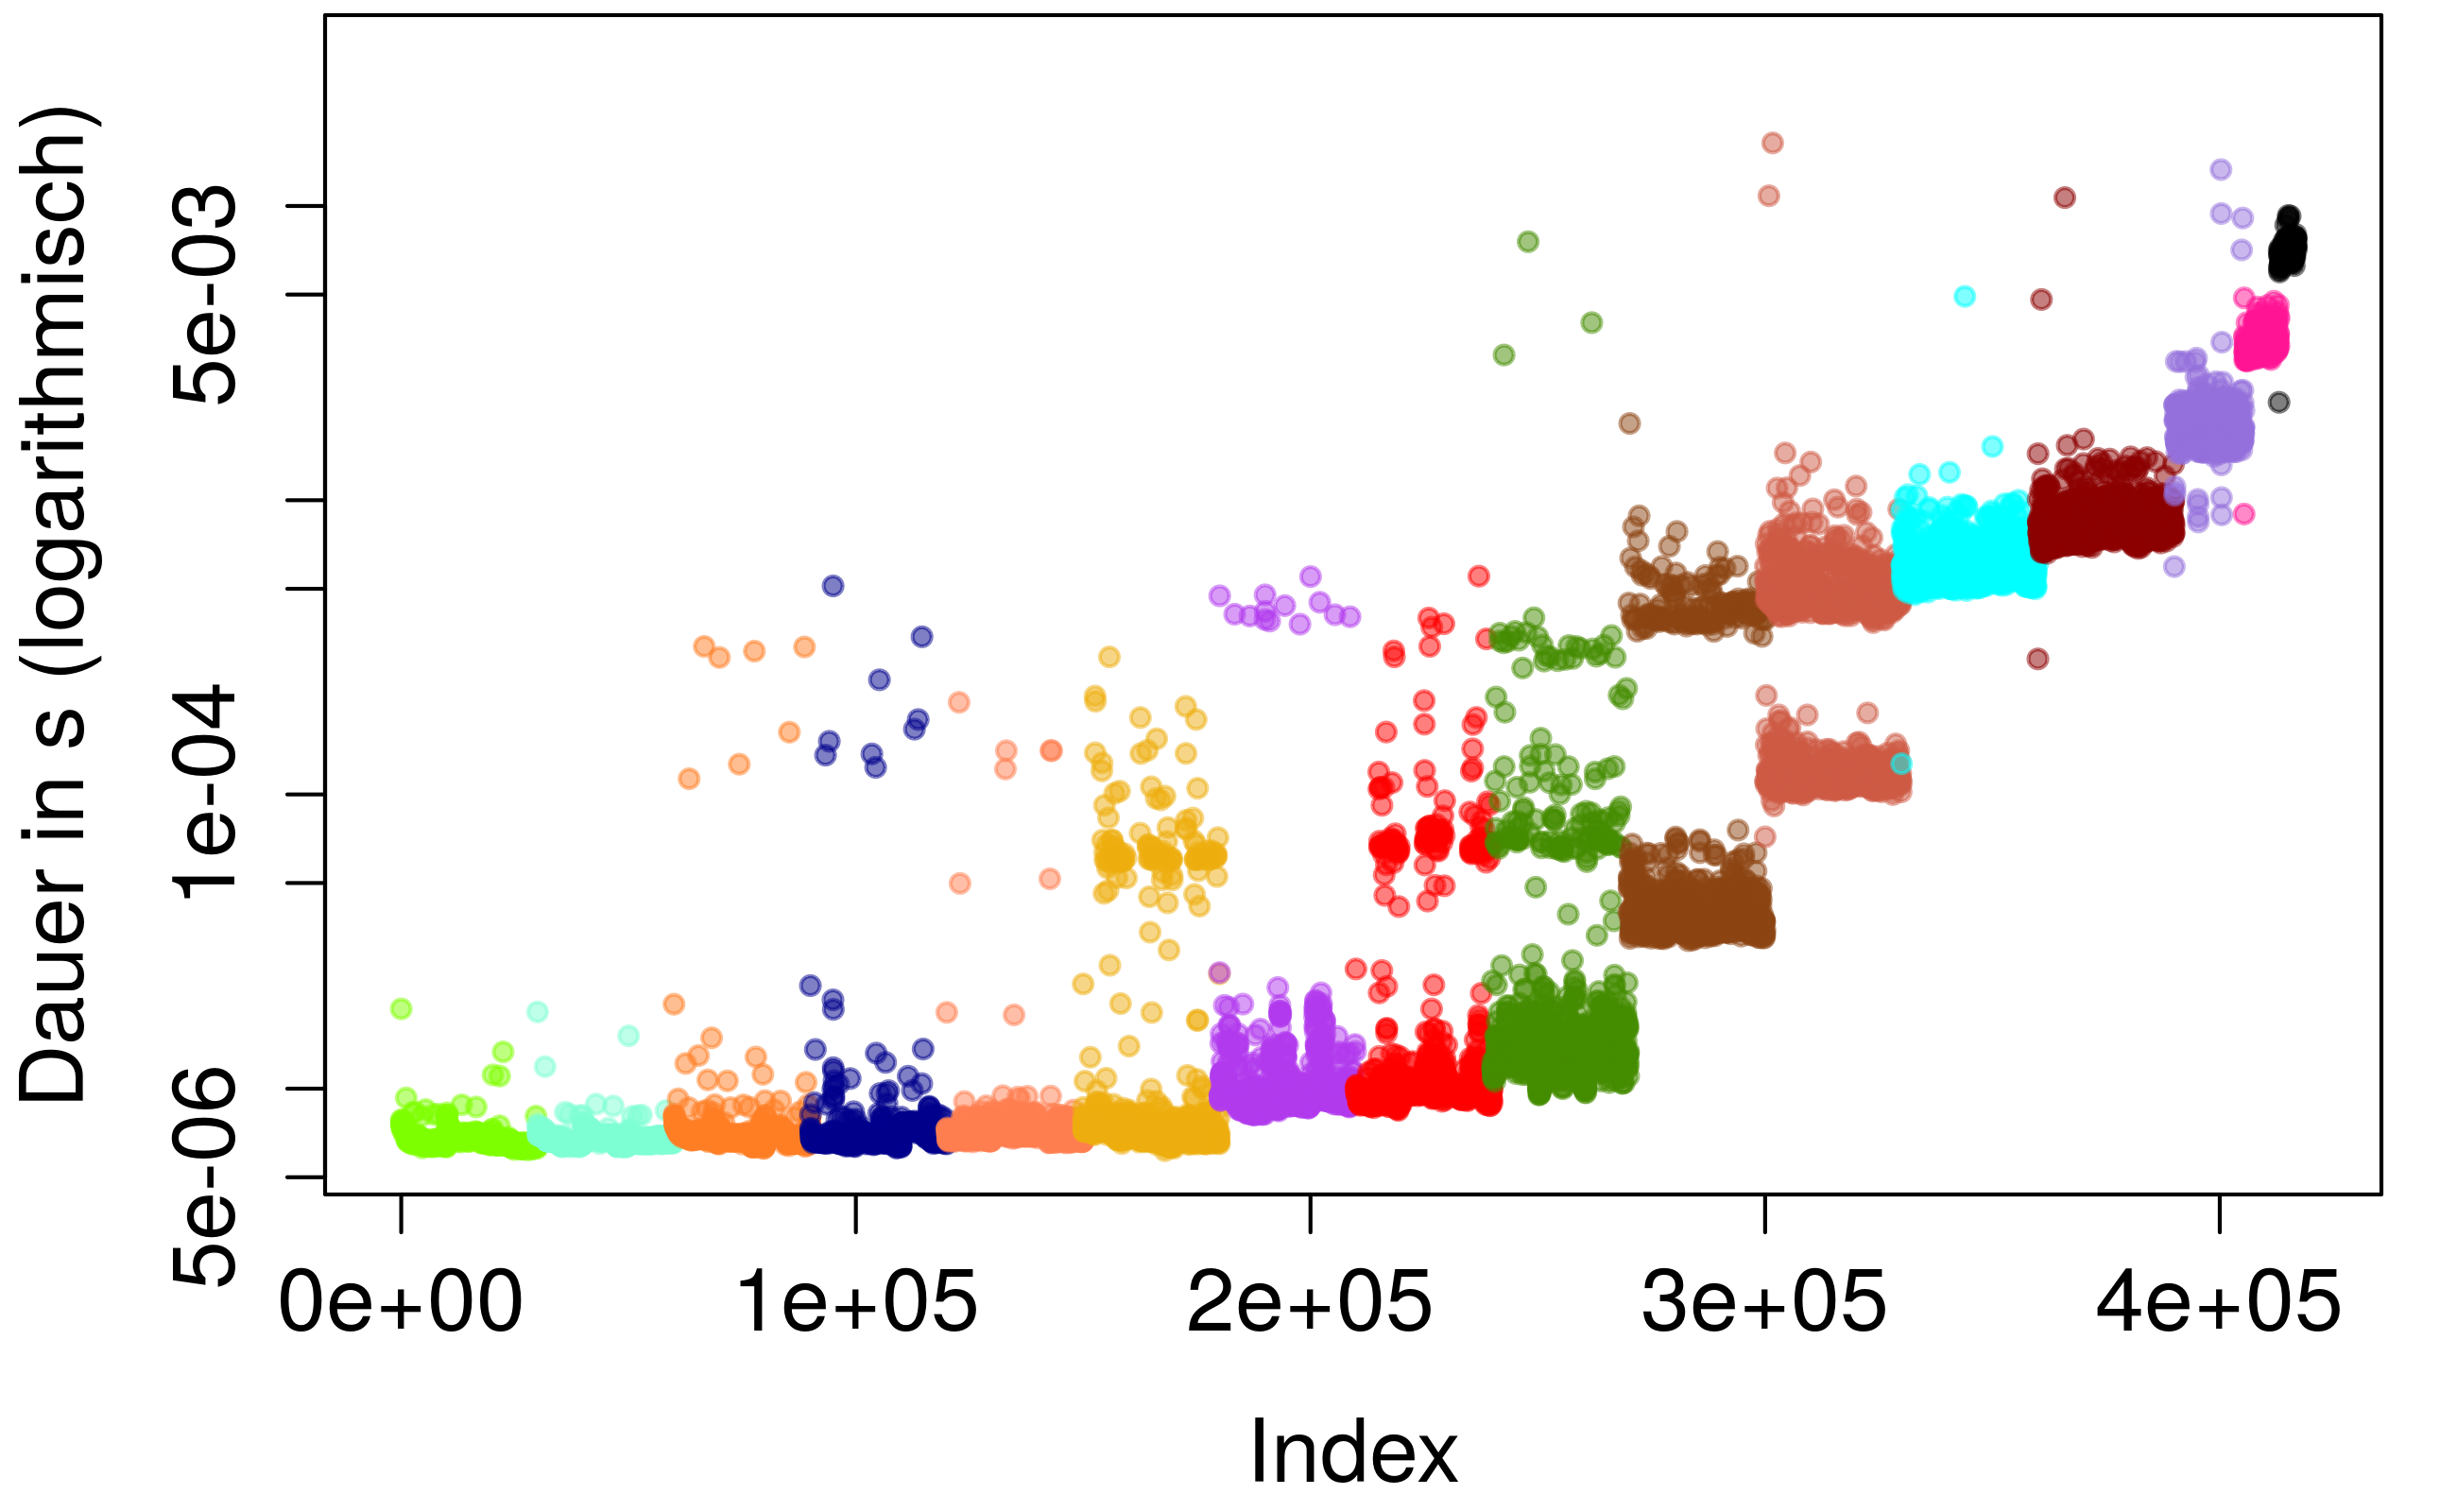
\includegraphics[width=.5\textwidth]{Bilder/Plots/exploration/plot_SizeSorted_log_read_seq.png}
	}
	\hfill
	\subfloat[Sequentiell schreibend]{
		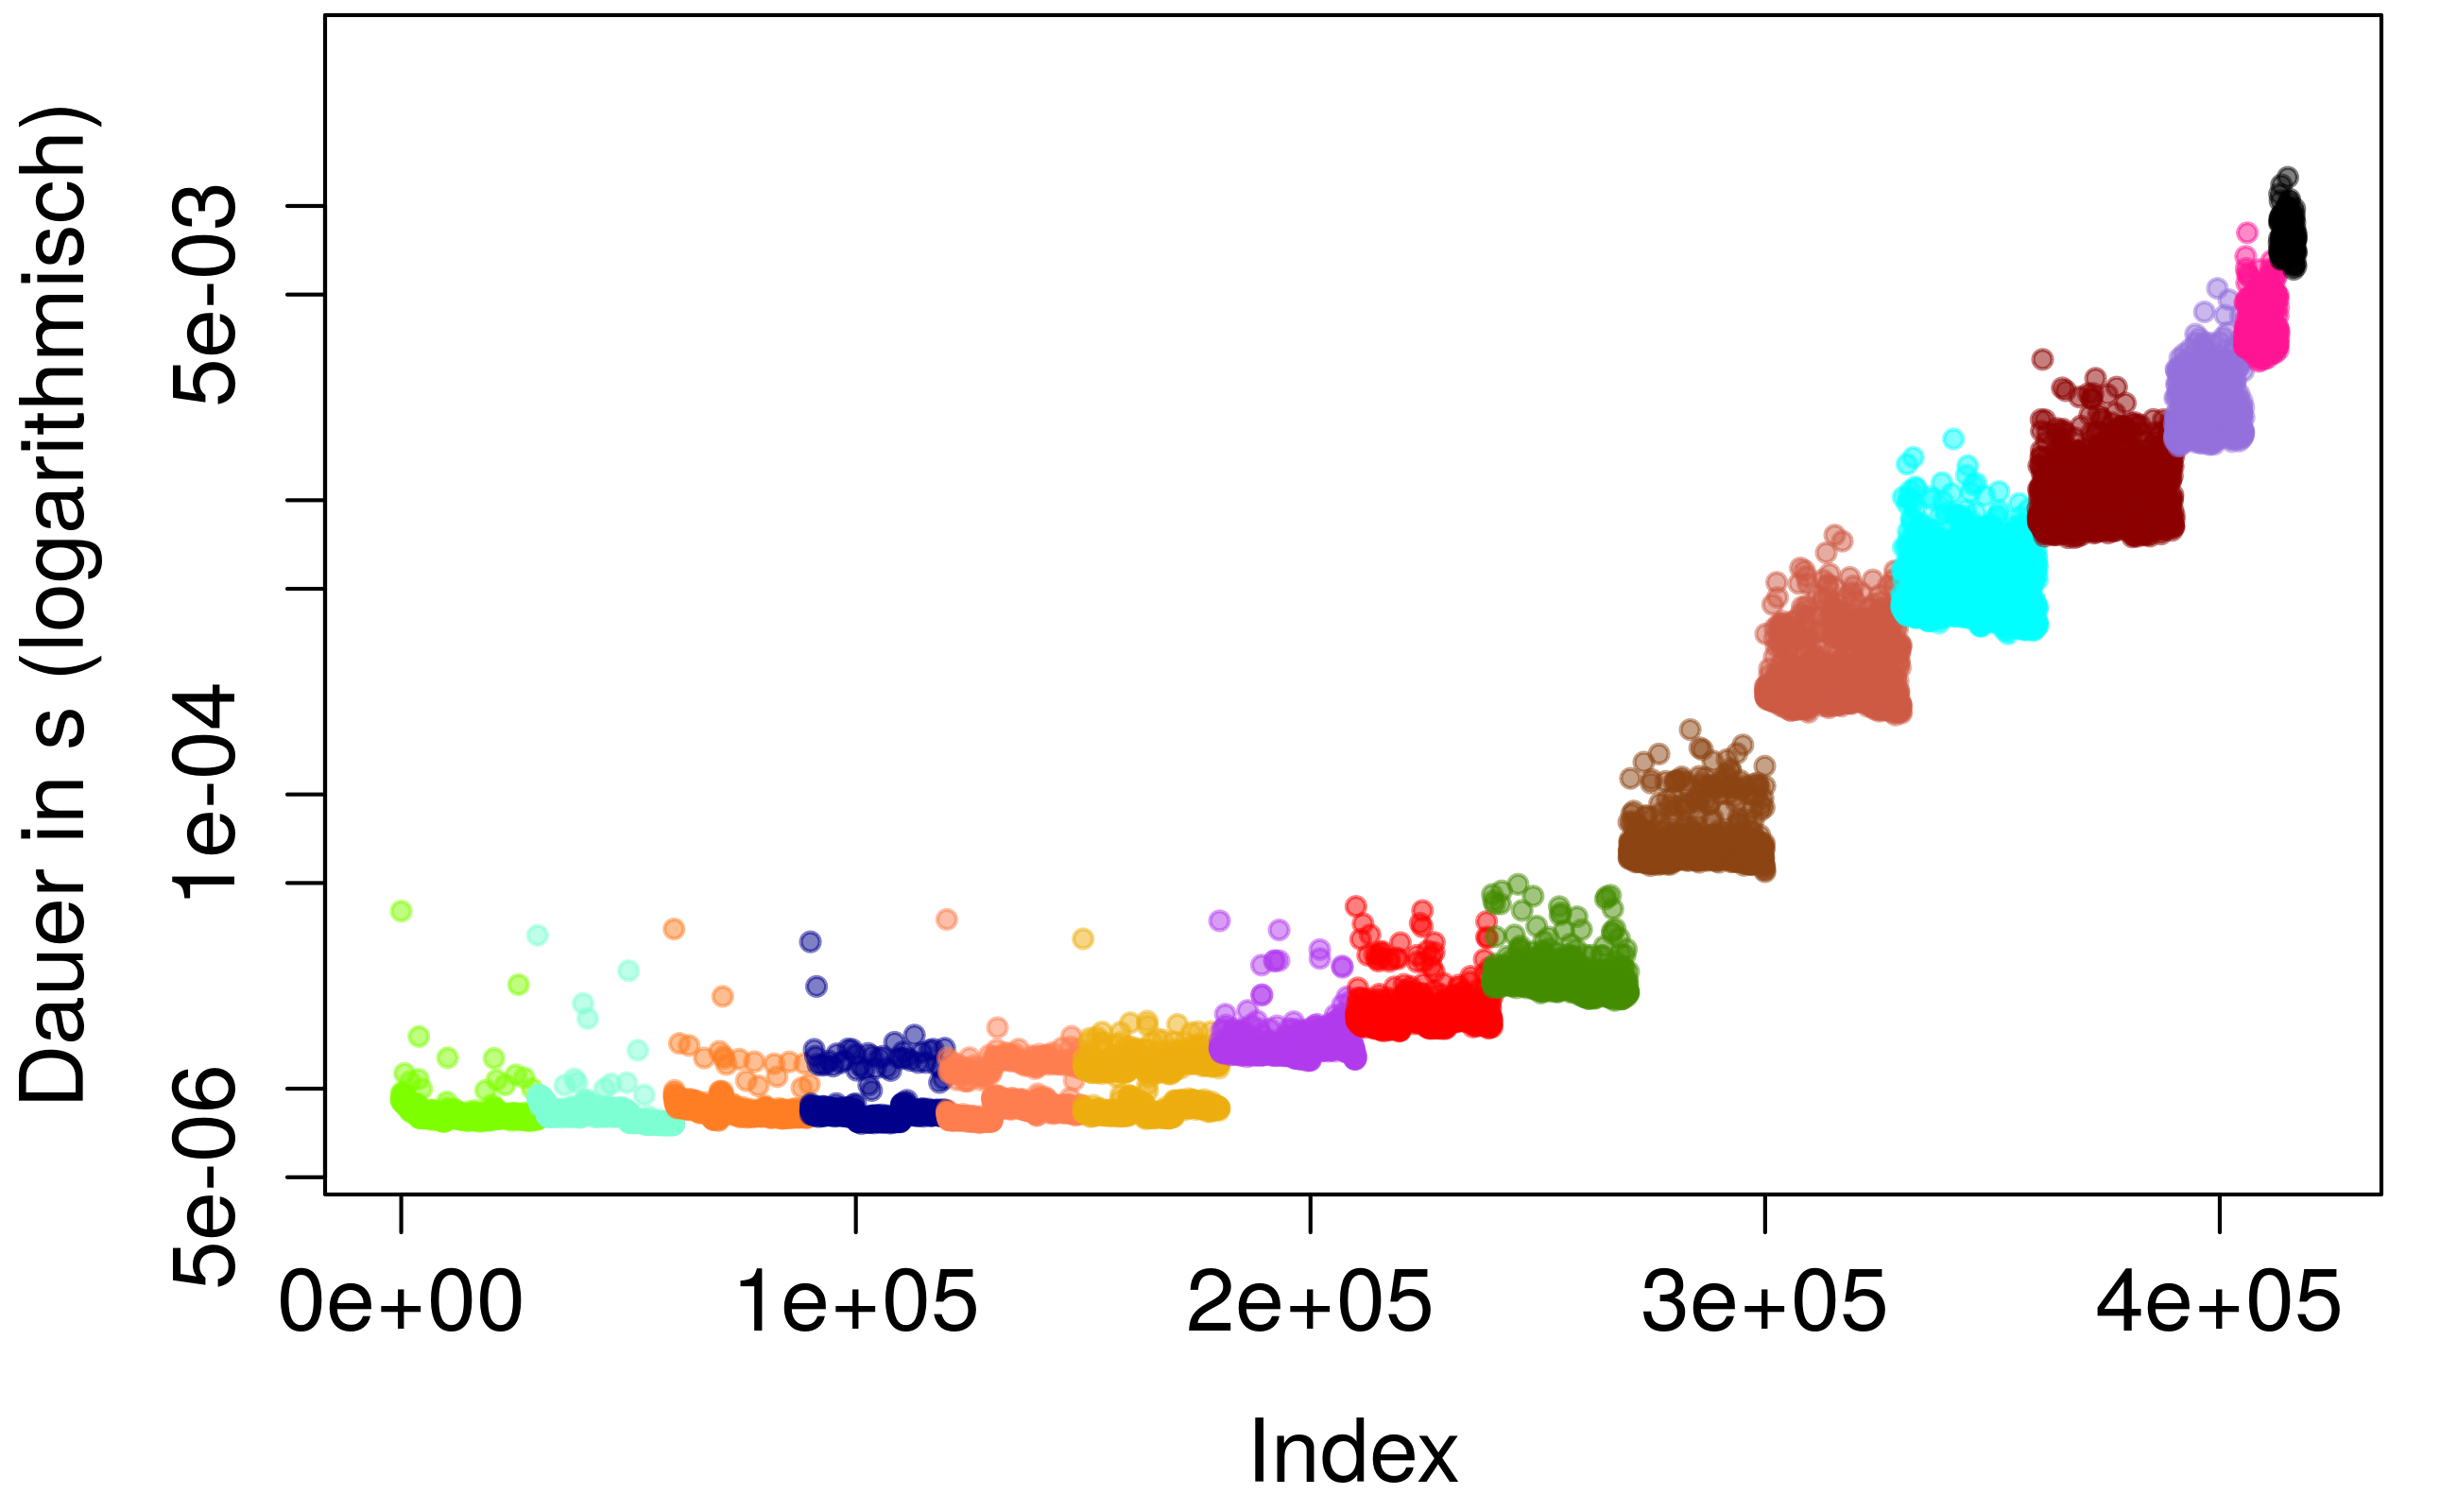
\includegraphics[width=.5\textwidth]{Bilder/Plots/exploration/plot_SizeSorted_log_write_seq.png}
	}\\
	\subfloat[Randomisiert lesend]{
		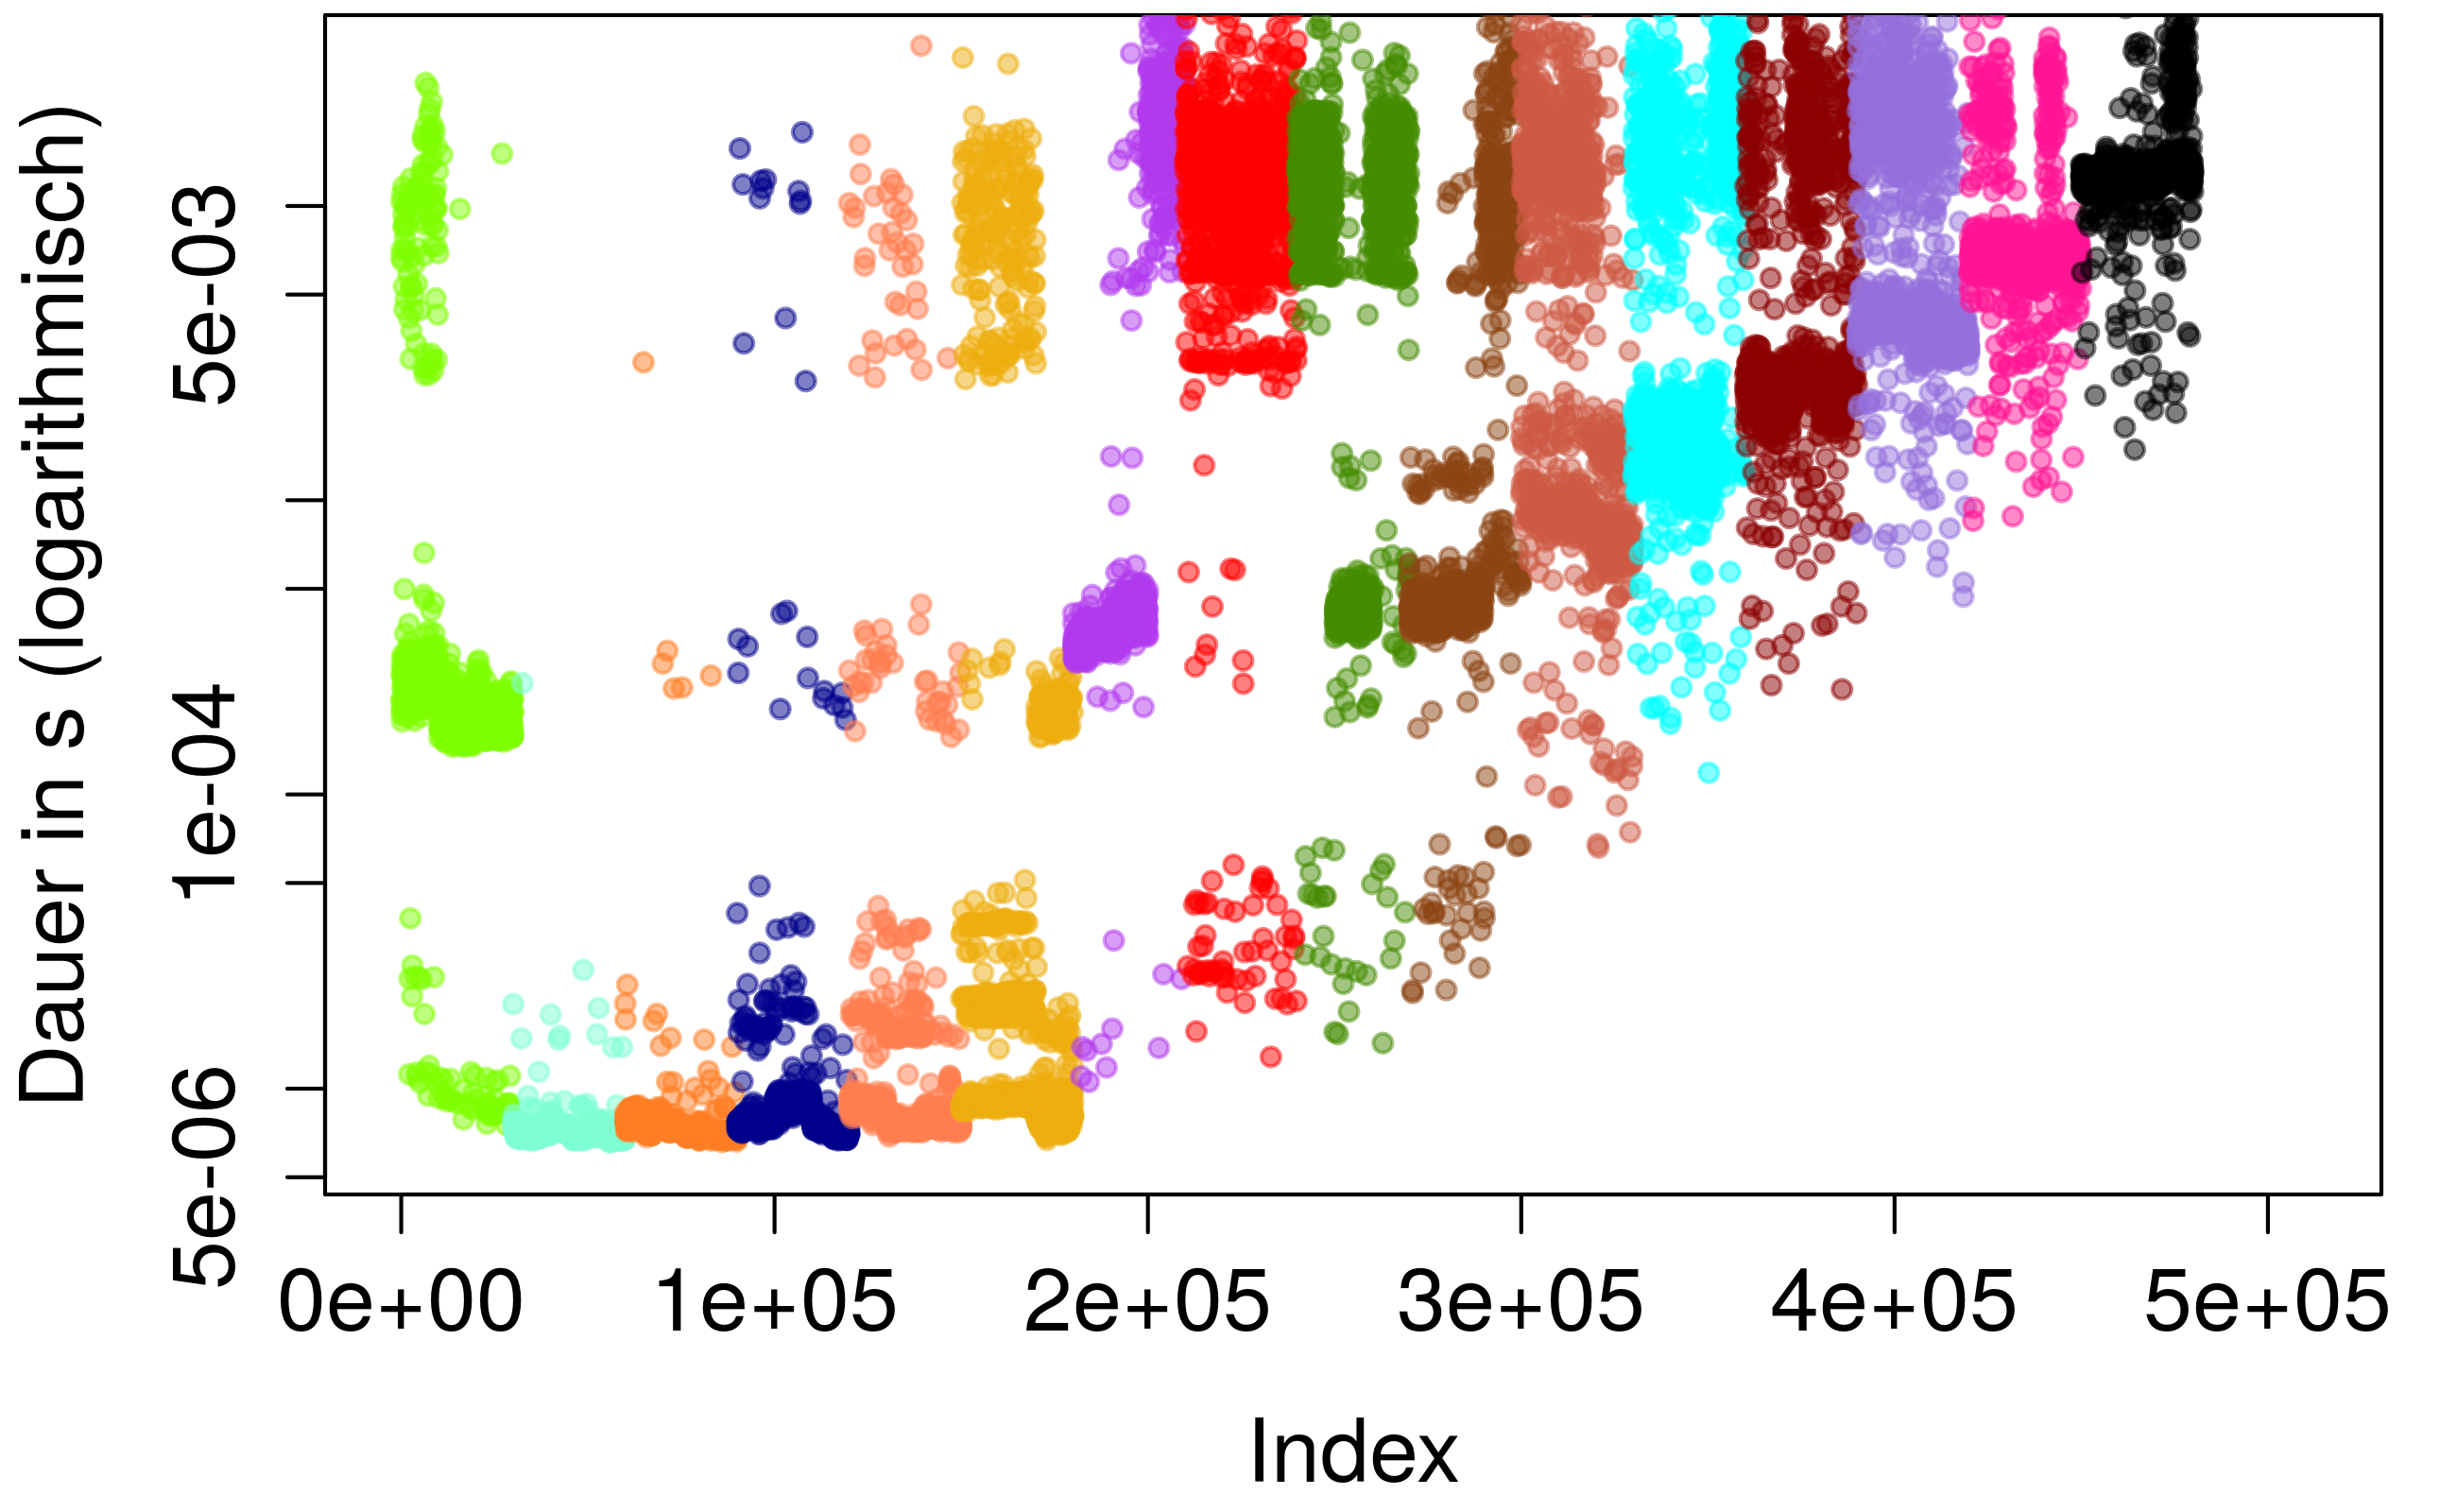
\includegraphics[width=.5\textwidth]{Bilder/Plots/exploration/plot_SizeSorted_log_read_rnd.png}
	}
	\hfill
	\subfloat[Randomisiert schreibend]{
		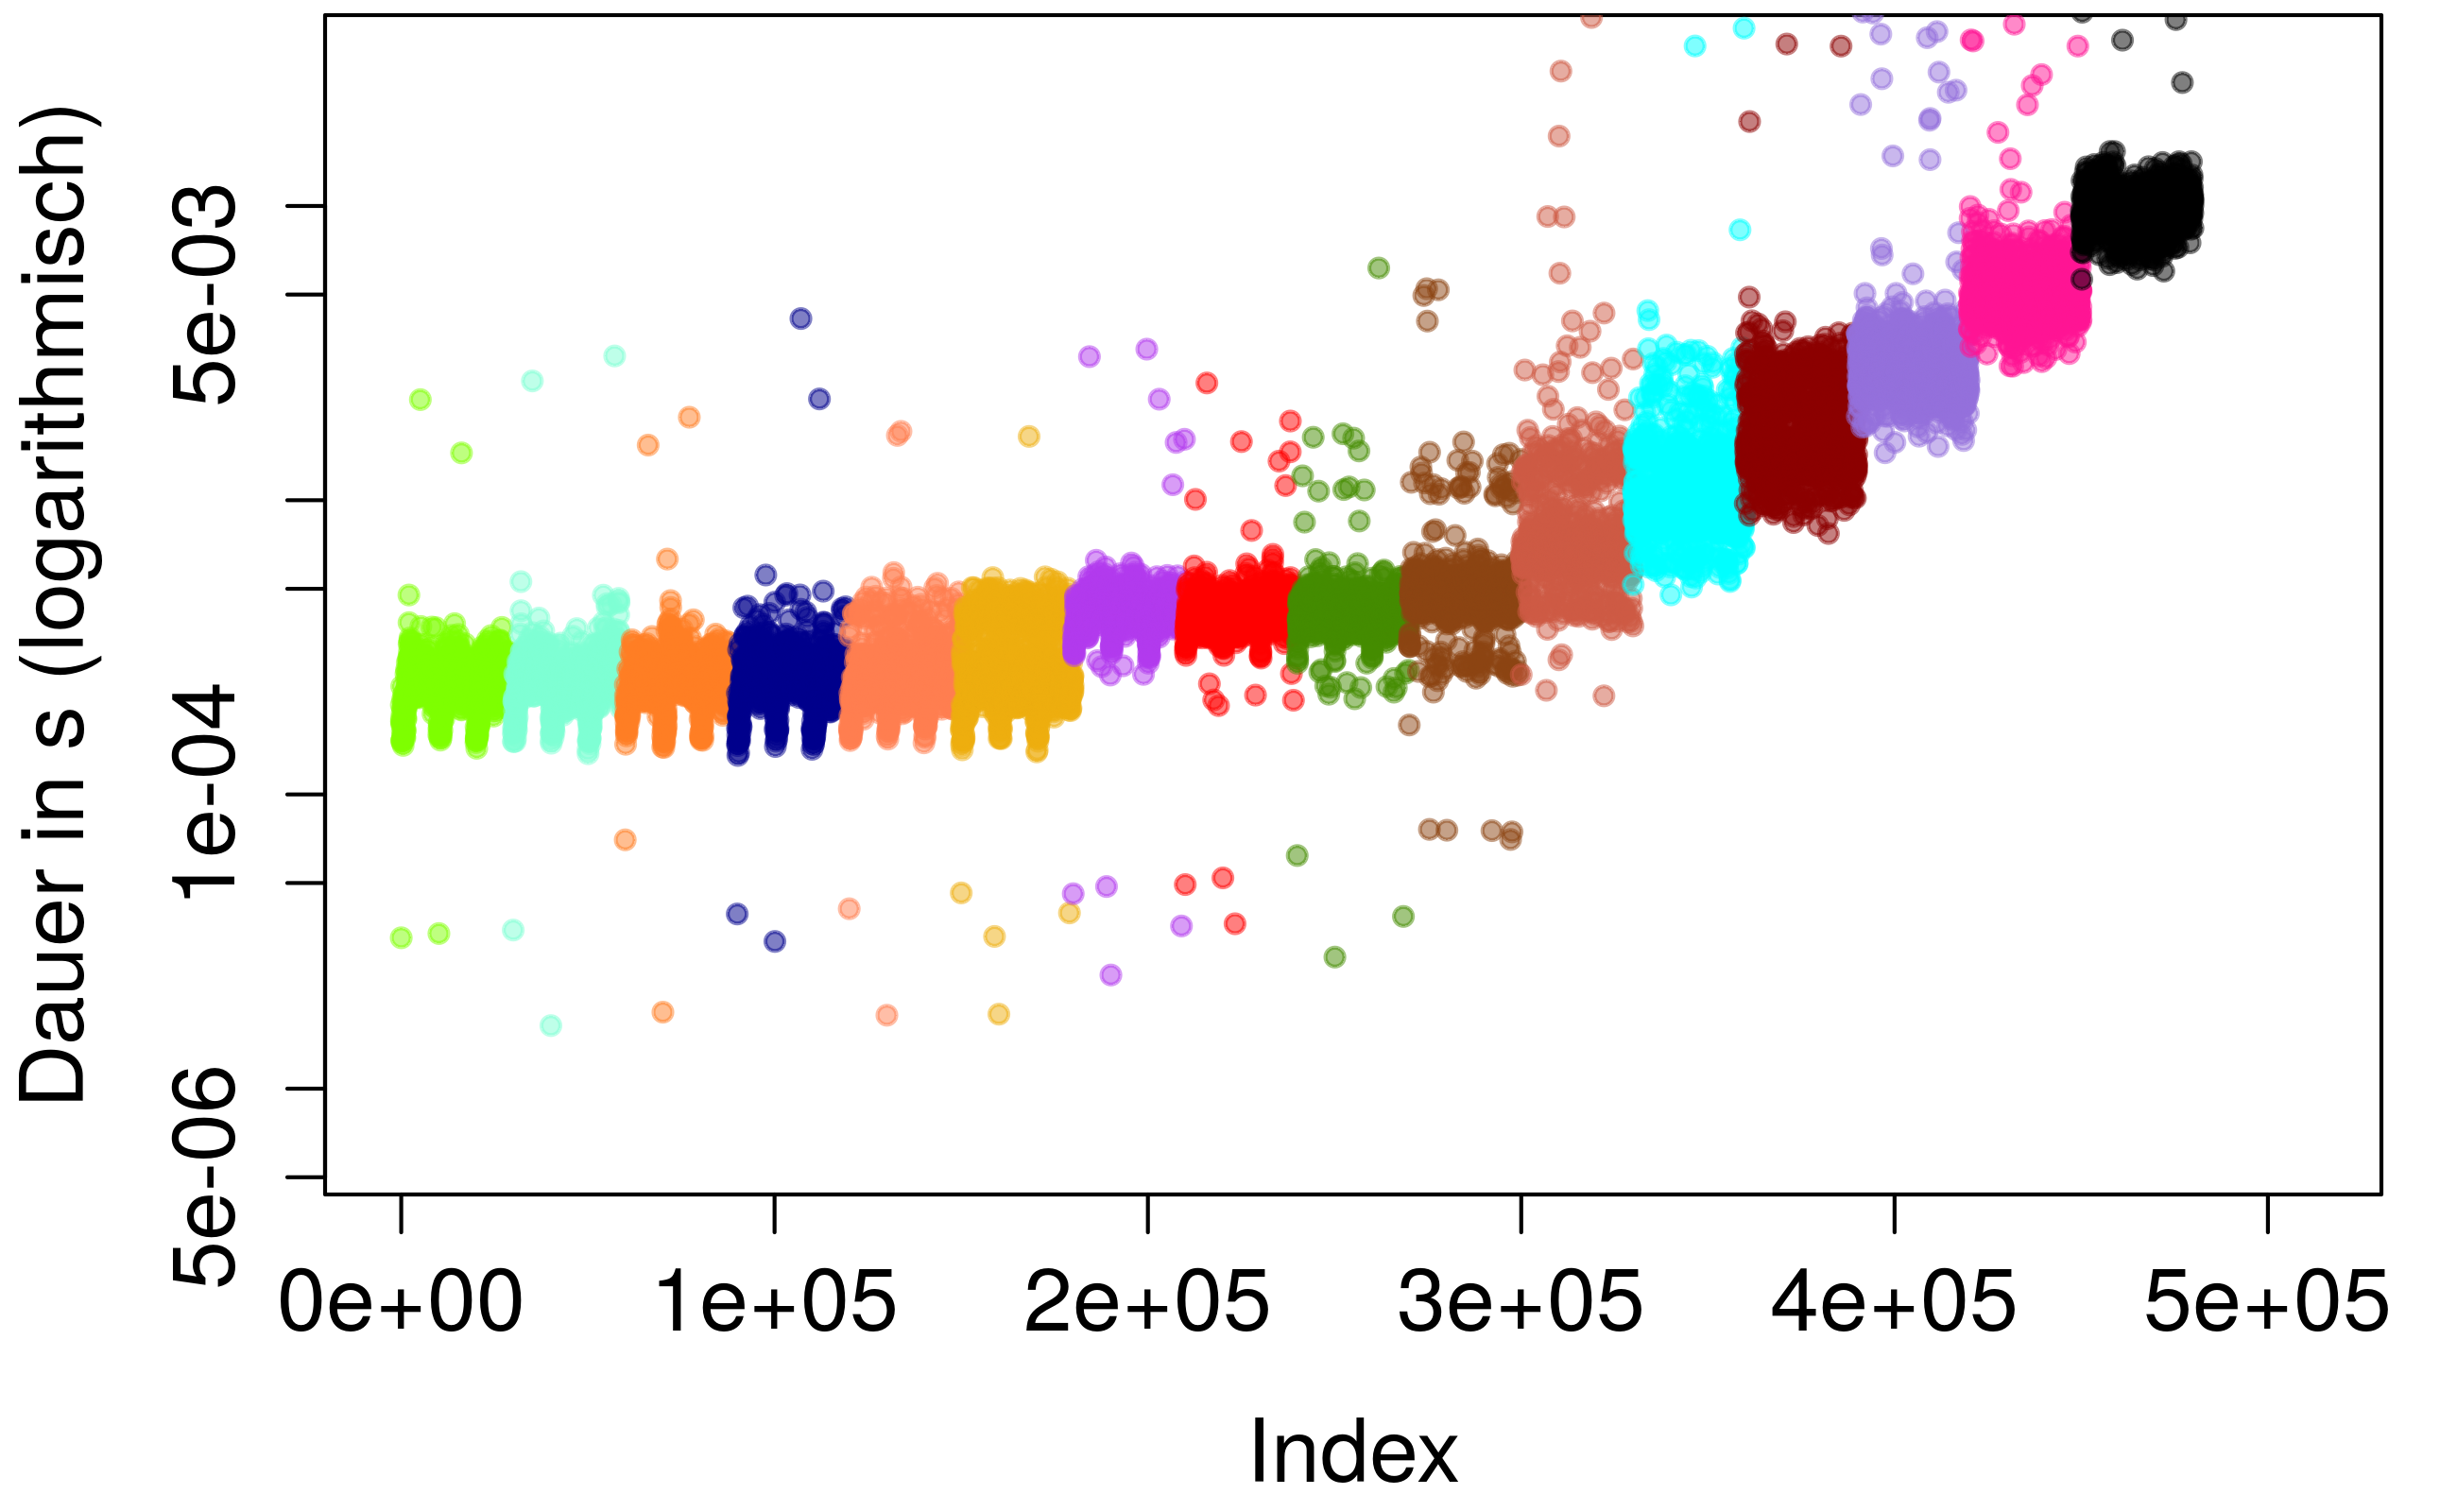
\includegraphics[width=.5\textwidth]{Bilder/Plots/exploration/plot_SizeSorted_log_write_rnd.png}
	}	
	\caption{Messungen der Laufzeiten nach Zugriffsgröße sortiert dargestellt. Von links nach rechts 1B, 4B, 16B, 64B, 256B, 1KiB, 4KiB, 8KiB, 16KiB, 64KiB, 256KiB, 512KiB, 1MiB, 2MiB, 4MiB, 8MiB und 16MiB}
	\label{Laufzeiten_Zeitreihe}
\end{figure} 

Wenn die Messpunkte nach der Laufzeit sortiert sind (\ref{Laufzeiten_Sortiert}), kann Verteilung der Laufzeiten besser betrachtet werden.
Insbesondere sind in dieser Darstellung ein stufenartiger Verlauf ersichtlich.
Es scheint also bestimmte Laufzeiten zu geben, die gehäuft vorkommen, die sich als Auftritt der Stufen kennzeichnen. Andere Laufzeiten kommen dagegen seltener vor, sie bilden eine Senkrechte.
Einzelne stufen stammen einerseits von Zugriffsgrößen, die alle eine ähnliche Zugriffszeit haben, andere lassen sich als die vorhergesagten E/A-Pfade im System interpretieren.
So sind die Zugriffszeiten verschiedener Größen bei cached-off0-seq-W recht dicht, sodass sich die Stufen dieser Herkunft zuordnen lassen.
Der andere Fall lässt sich gut bei cached-off0-rnd-R erkennen. Die Zugriffszeiten zu einer Größe teilen sich bei \ref{Laufzeiten_Zeitreihe} in etwa drei Gruppen auf, eine langsame, eine mittlere und eine schnelle.
Die Gruppen verschiedener Zugriffsgrößen können teilweise zu einem E/A-Pfad zusammengefasst werden. Die Häufungen finden sich dann auf einer horizontalen Linie. 
Die Laufzeit ist für die horizontal nebeneinanderliegenden Gruppen nicht in erster Linie von der Zugriffsgröße abhängig, sondern in unserer Interpretation von dem Pfad, den die entsprechenden Aufrufe im System genommen haben. 

\begin{figure}
	\subfloat[Sequentiell lesend]{
		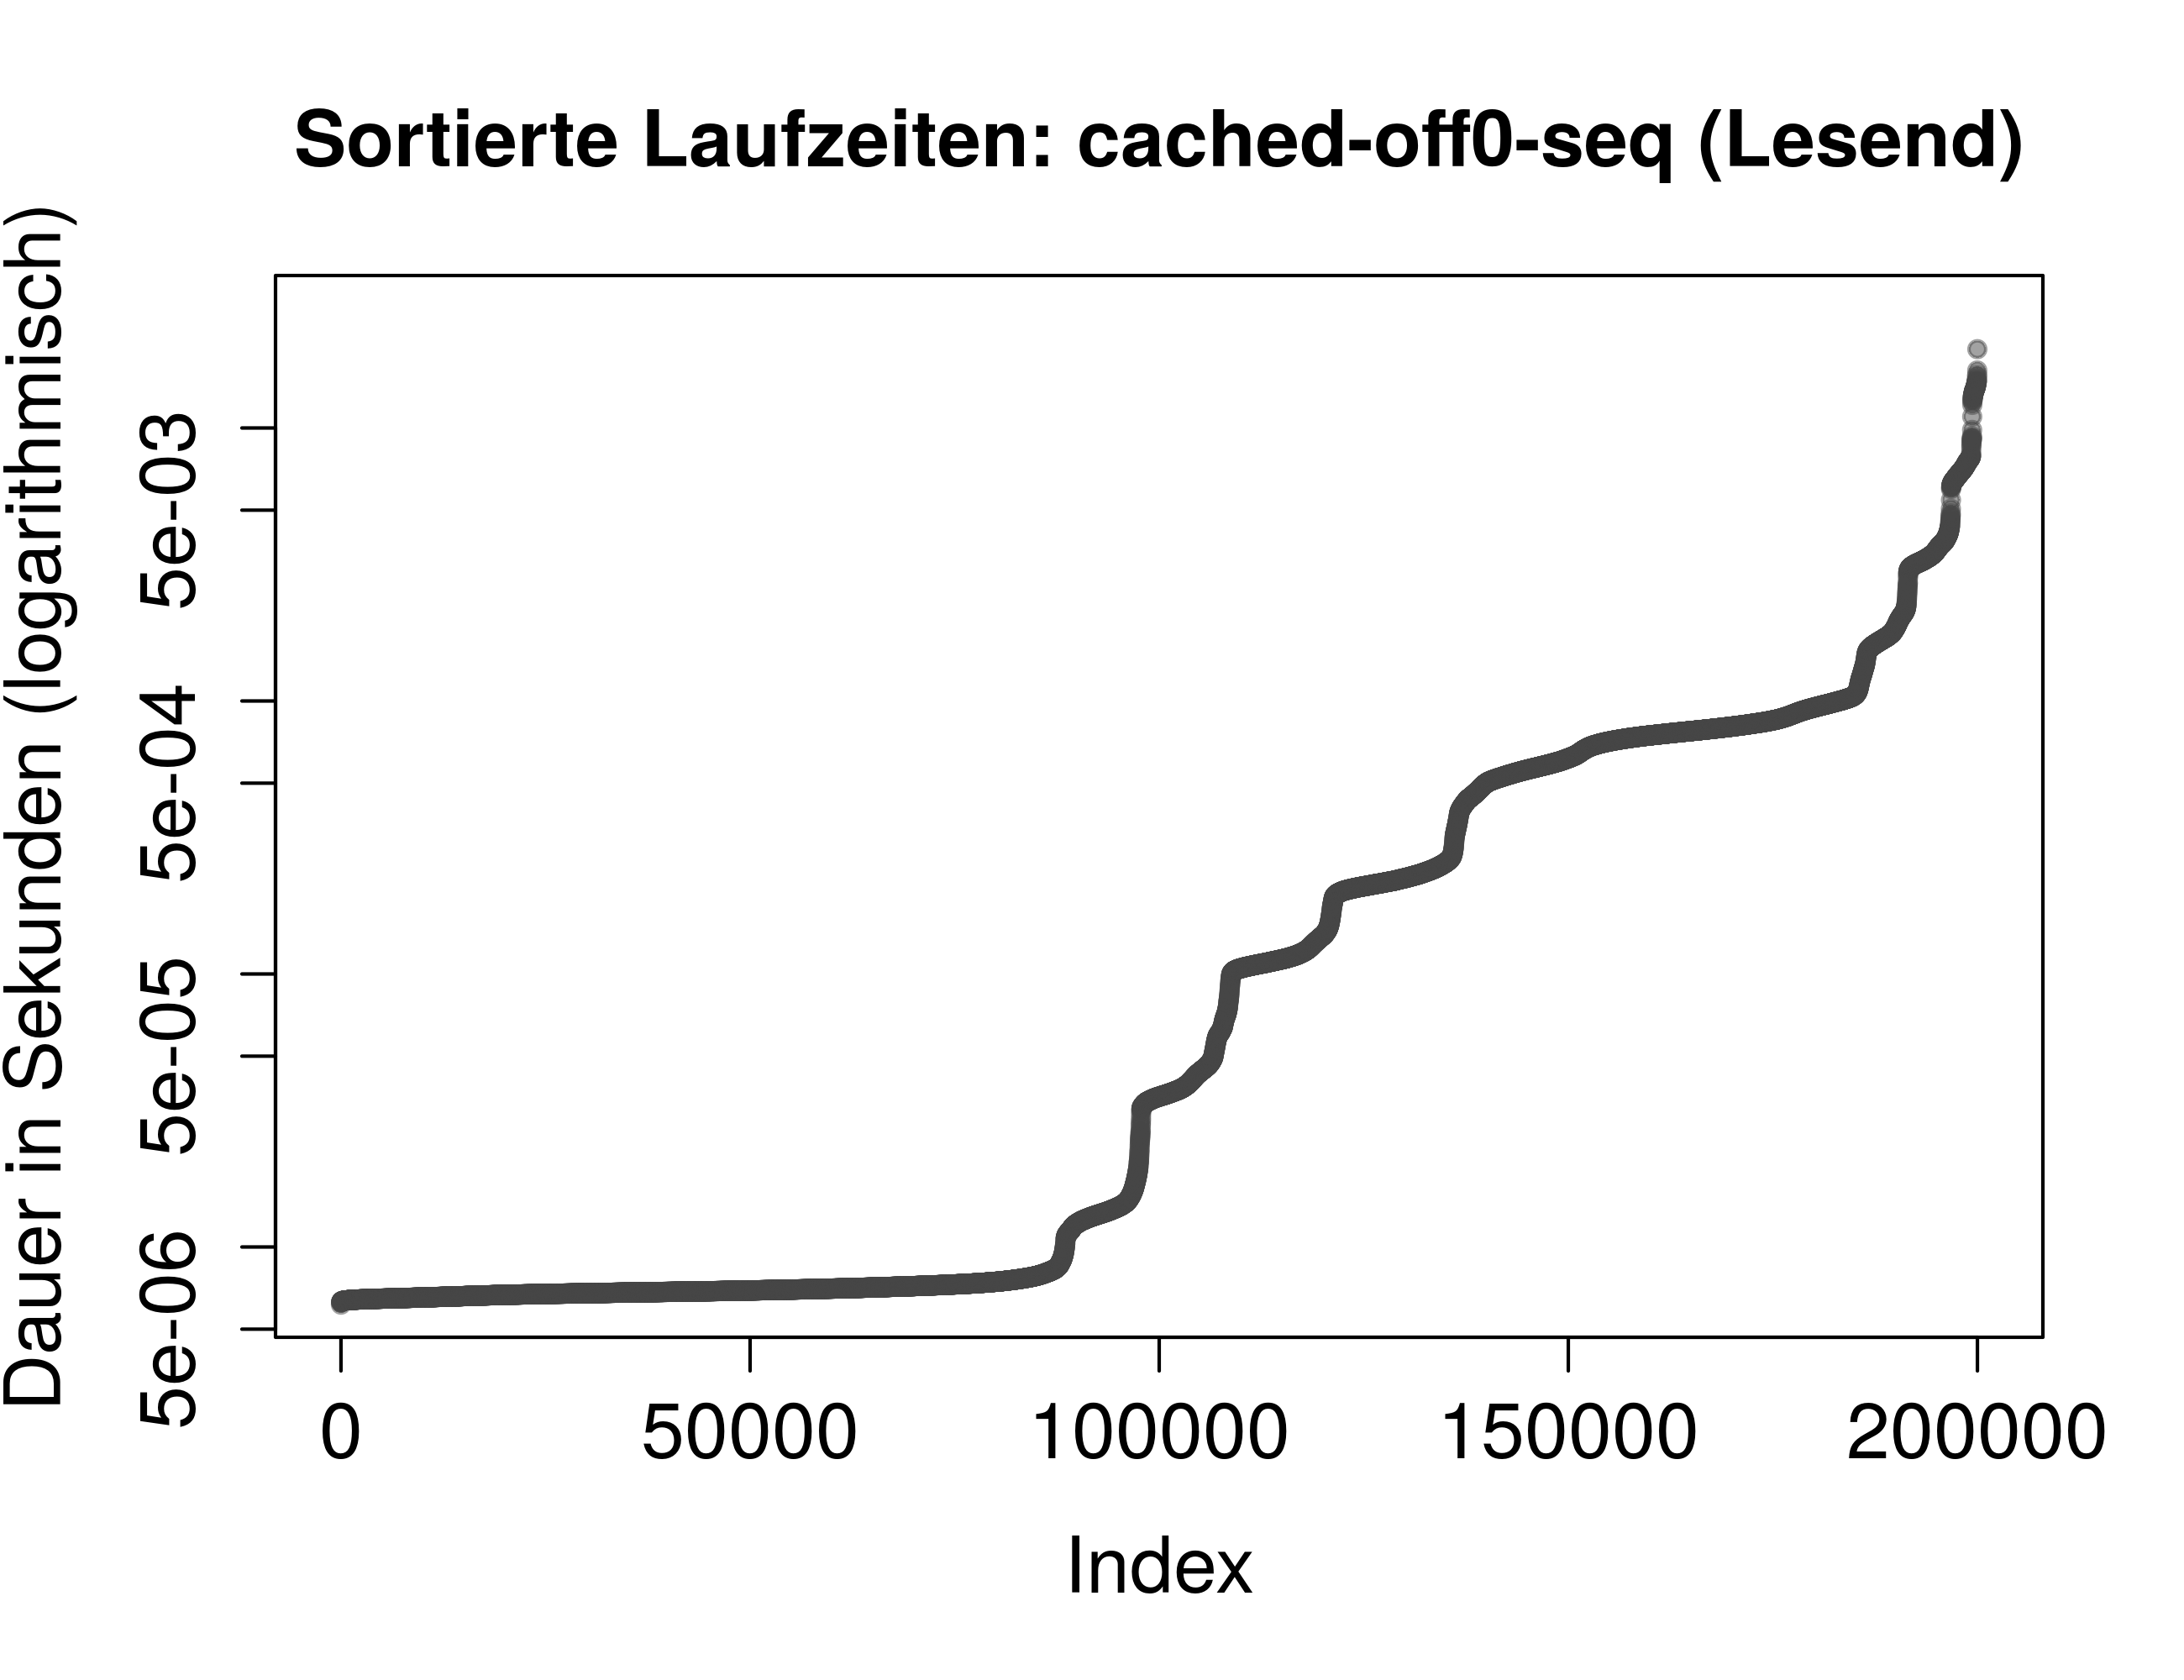
\includegraphics[width=.43\textwidth]{Bilder/Plots/exploration/plot_DurationSorted_read_seq.png}
	}
	\hfill
	\subfloat[Sequentiell schreibend]{
		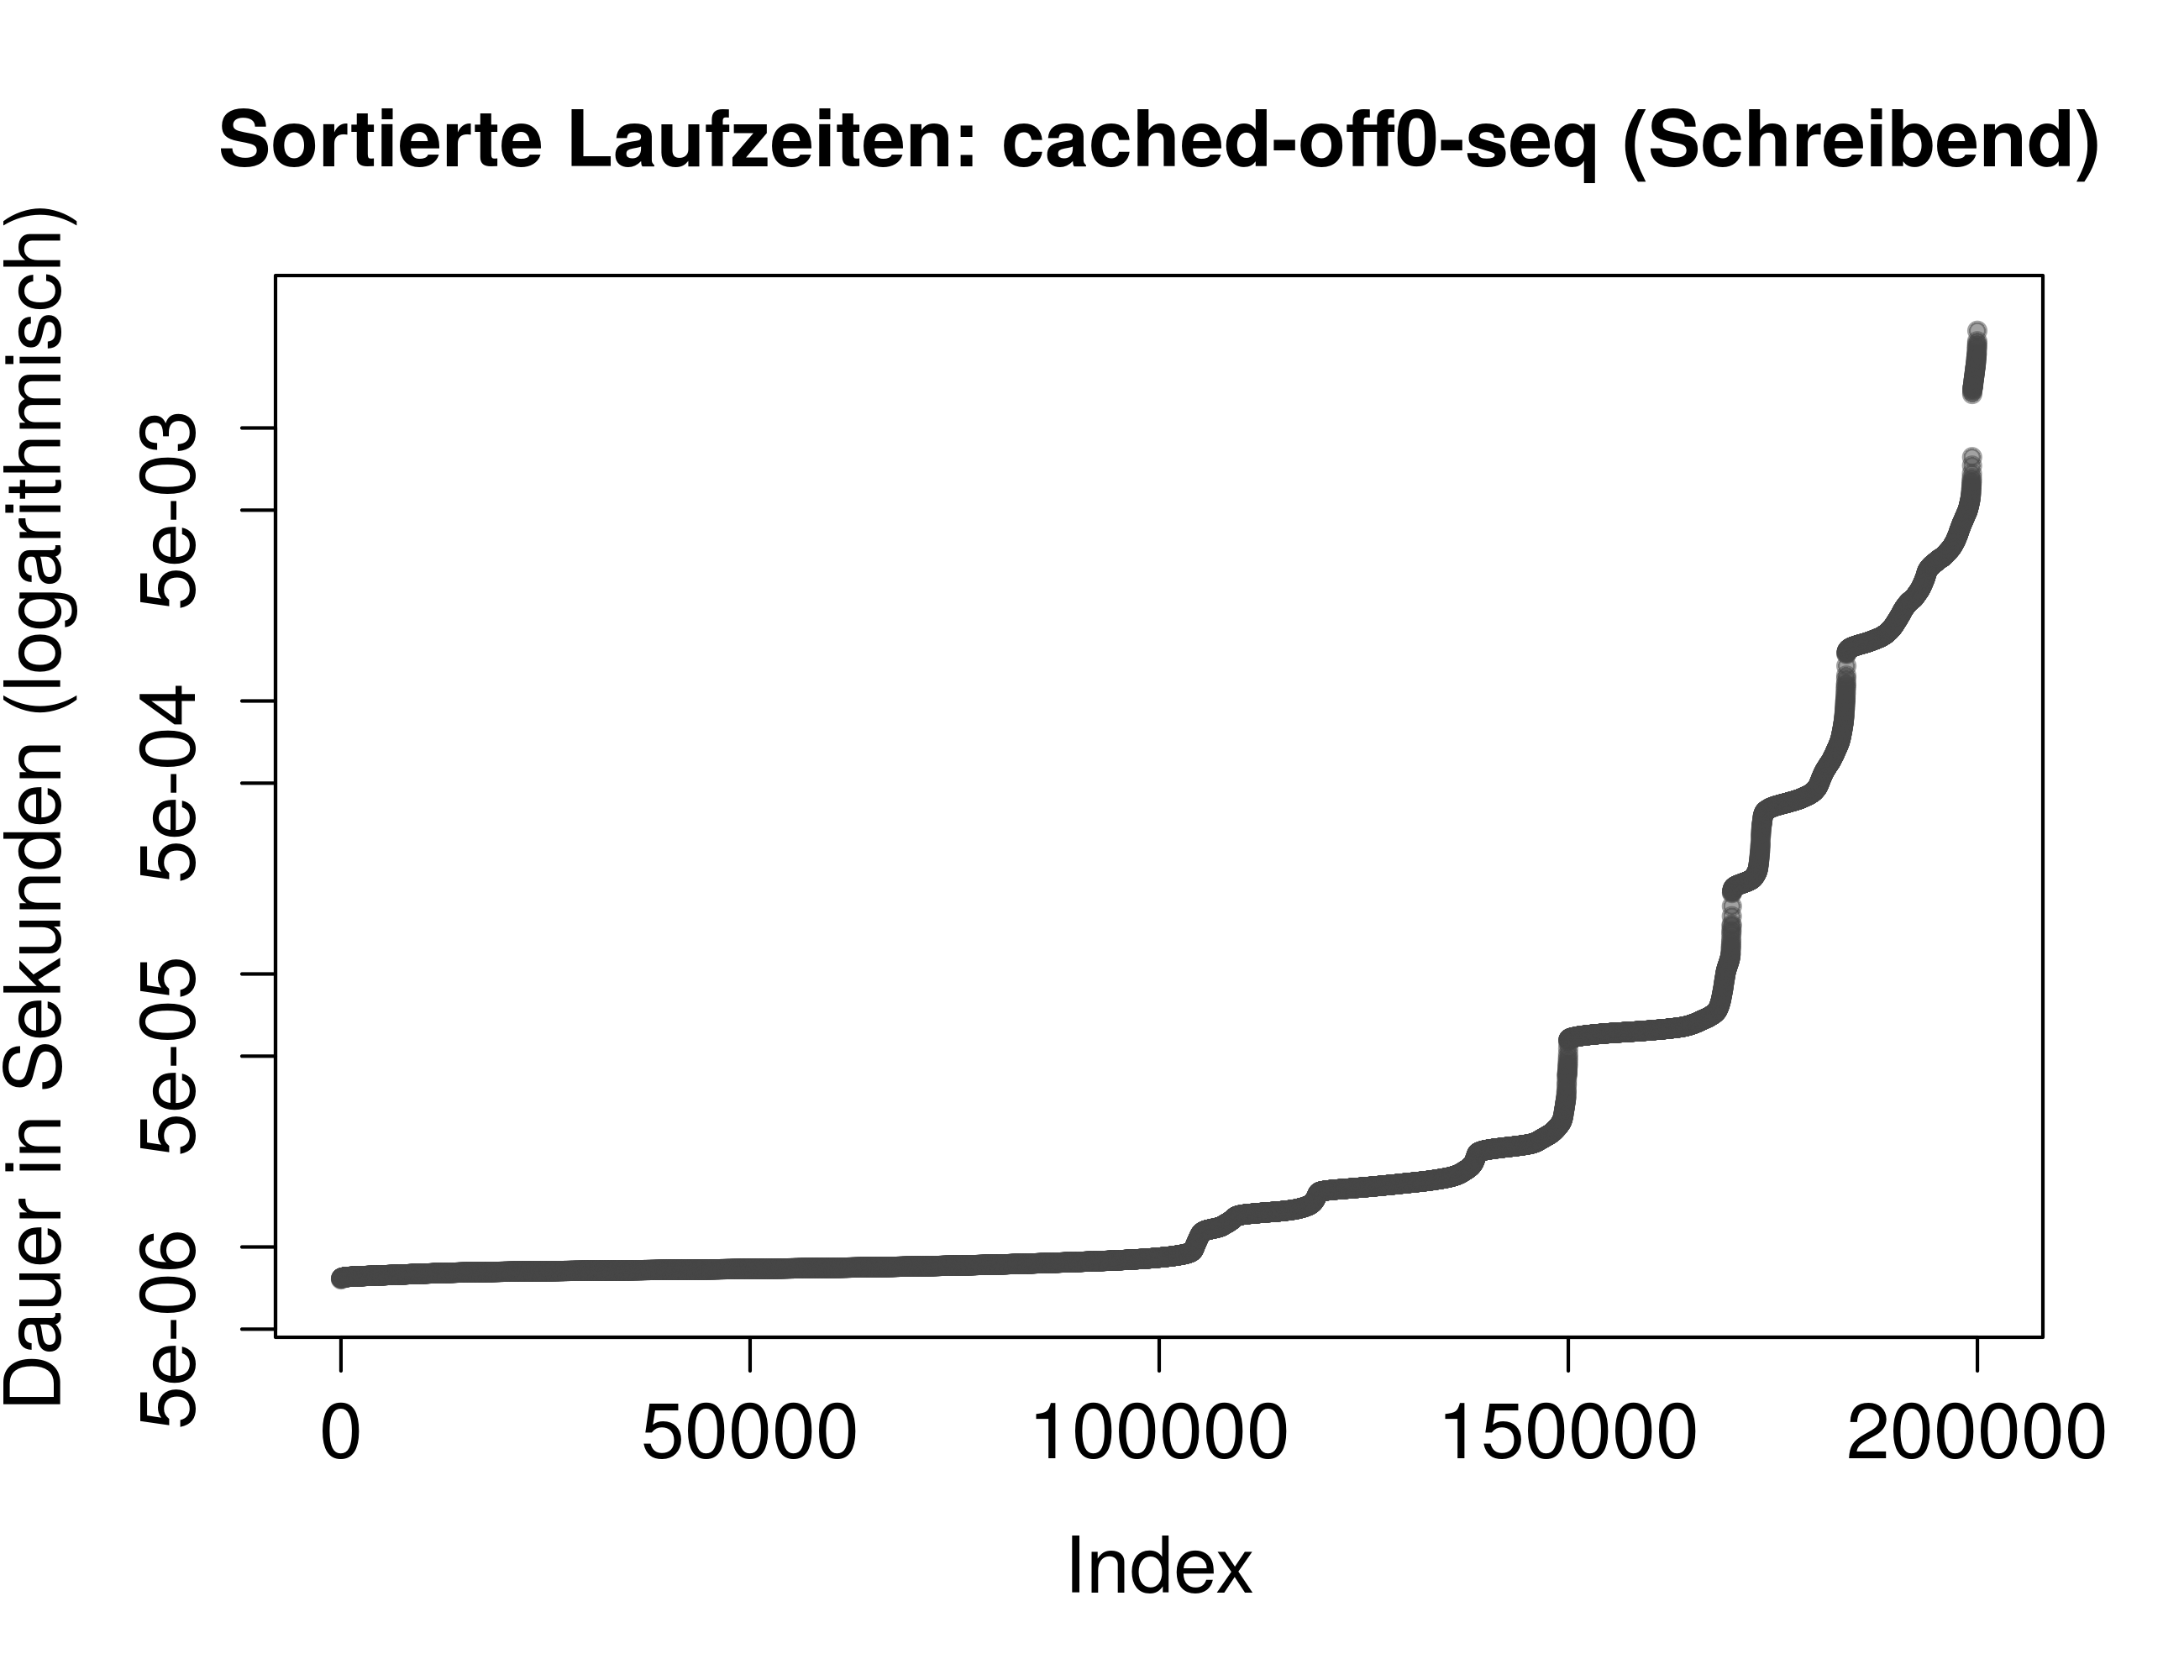
\includegraphics[width=.43\textwidth]{Bilder/Plots/exploration/plot_DurationSorted_write_seq.png}
	}\\
	\subfloat[Randomisiert lesend]{
		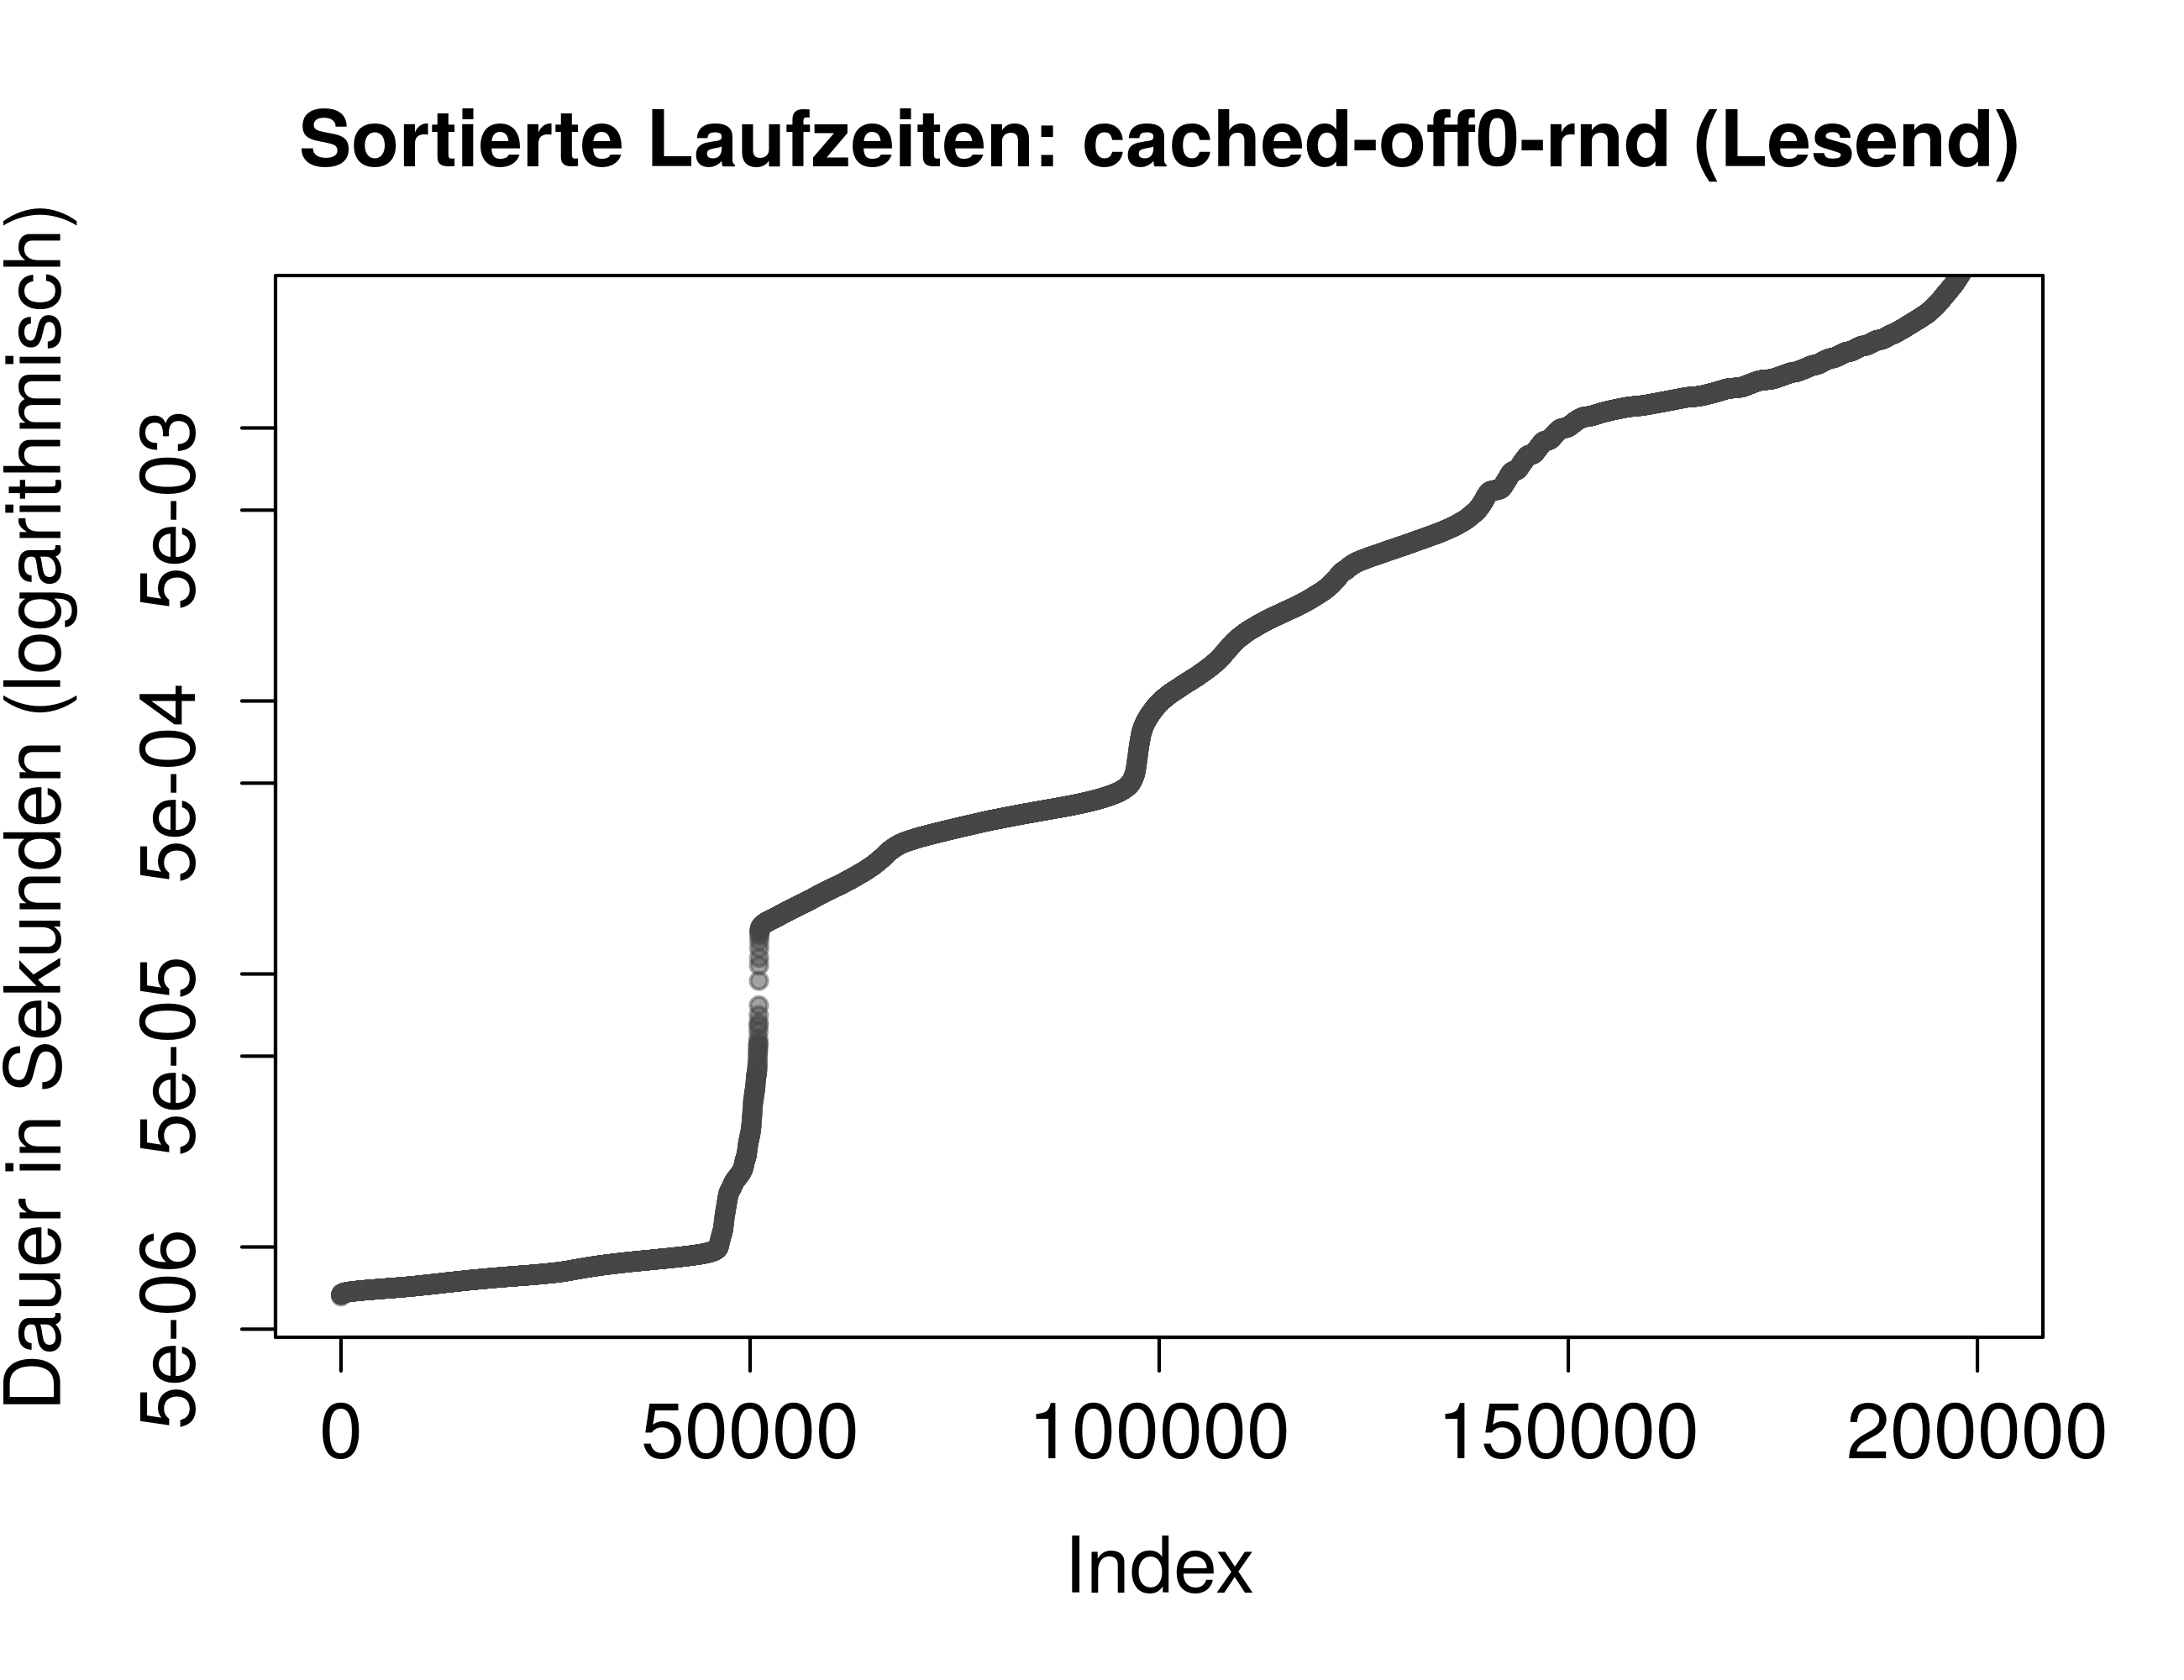
\includegraphics[width=.43\textwidth]{Bilder/Plots/exploration/plot_DurationSorted_read_rnd.png}
	}
	\hfill
	\subfloat[Randomisiert schreibend]{
		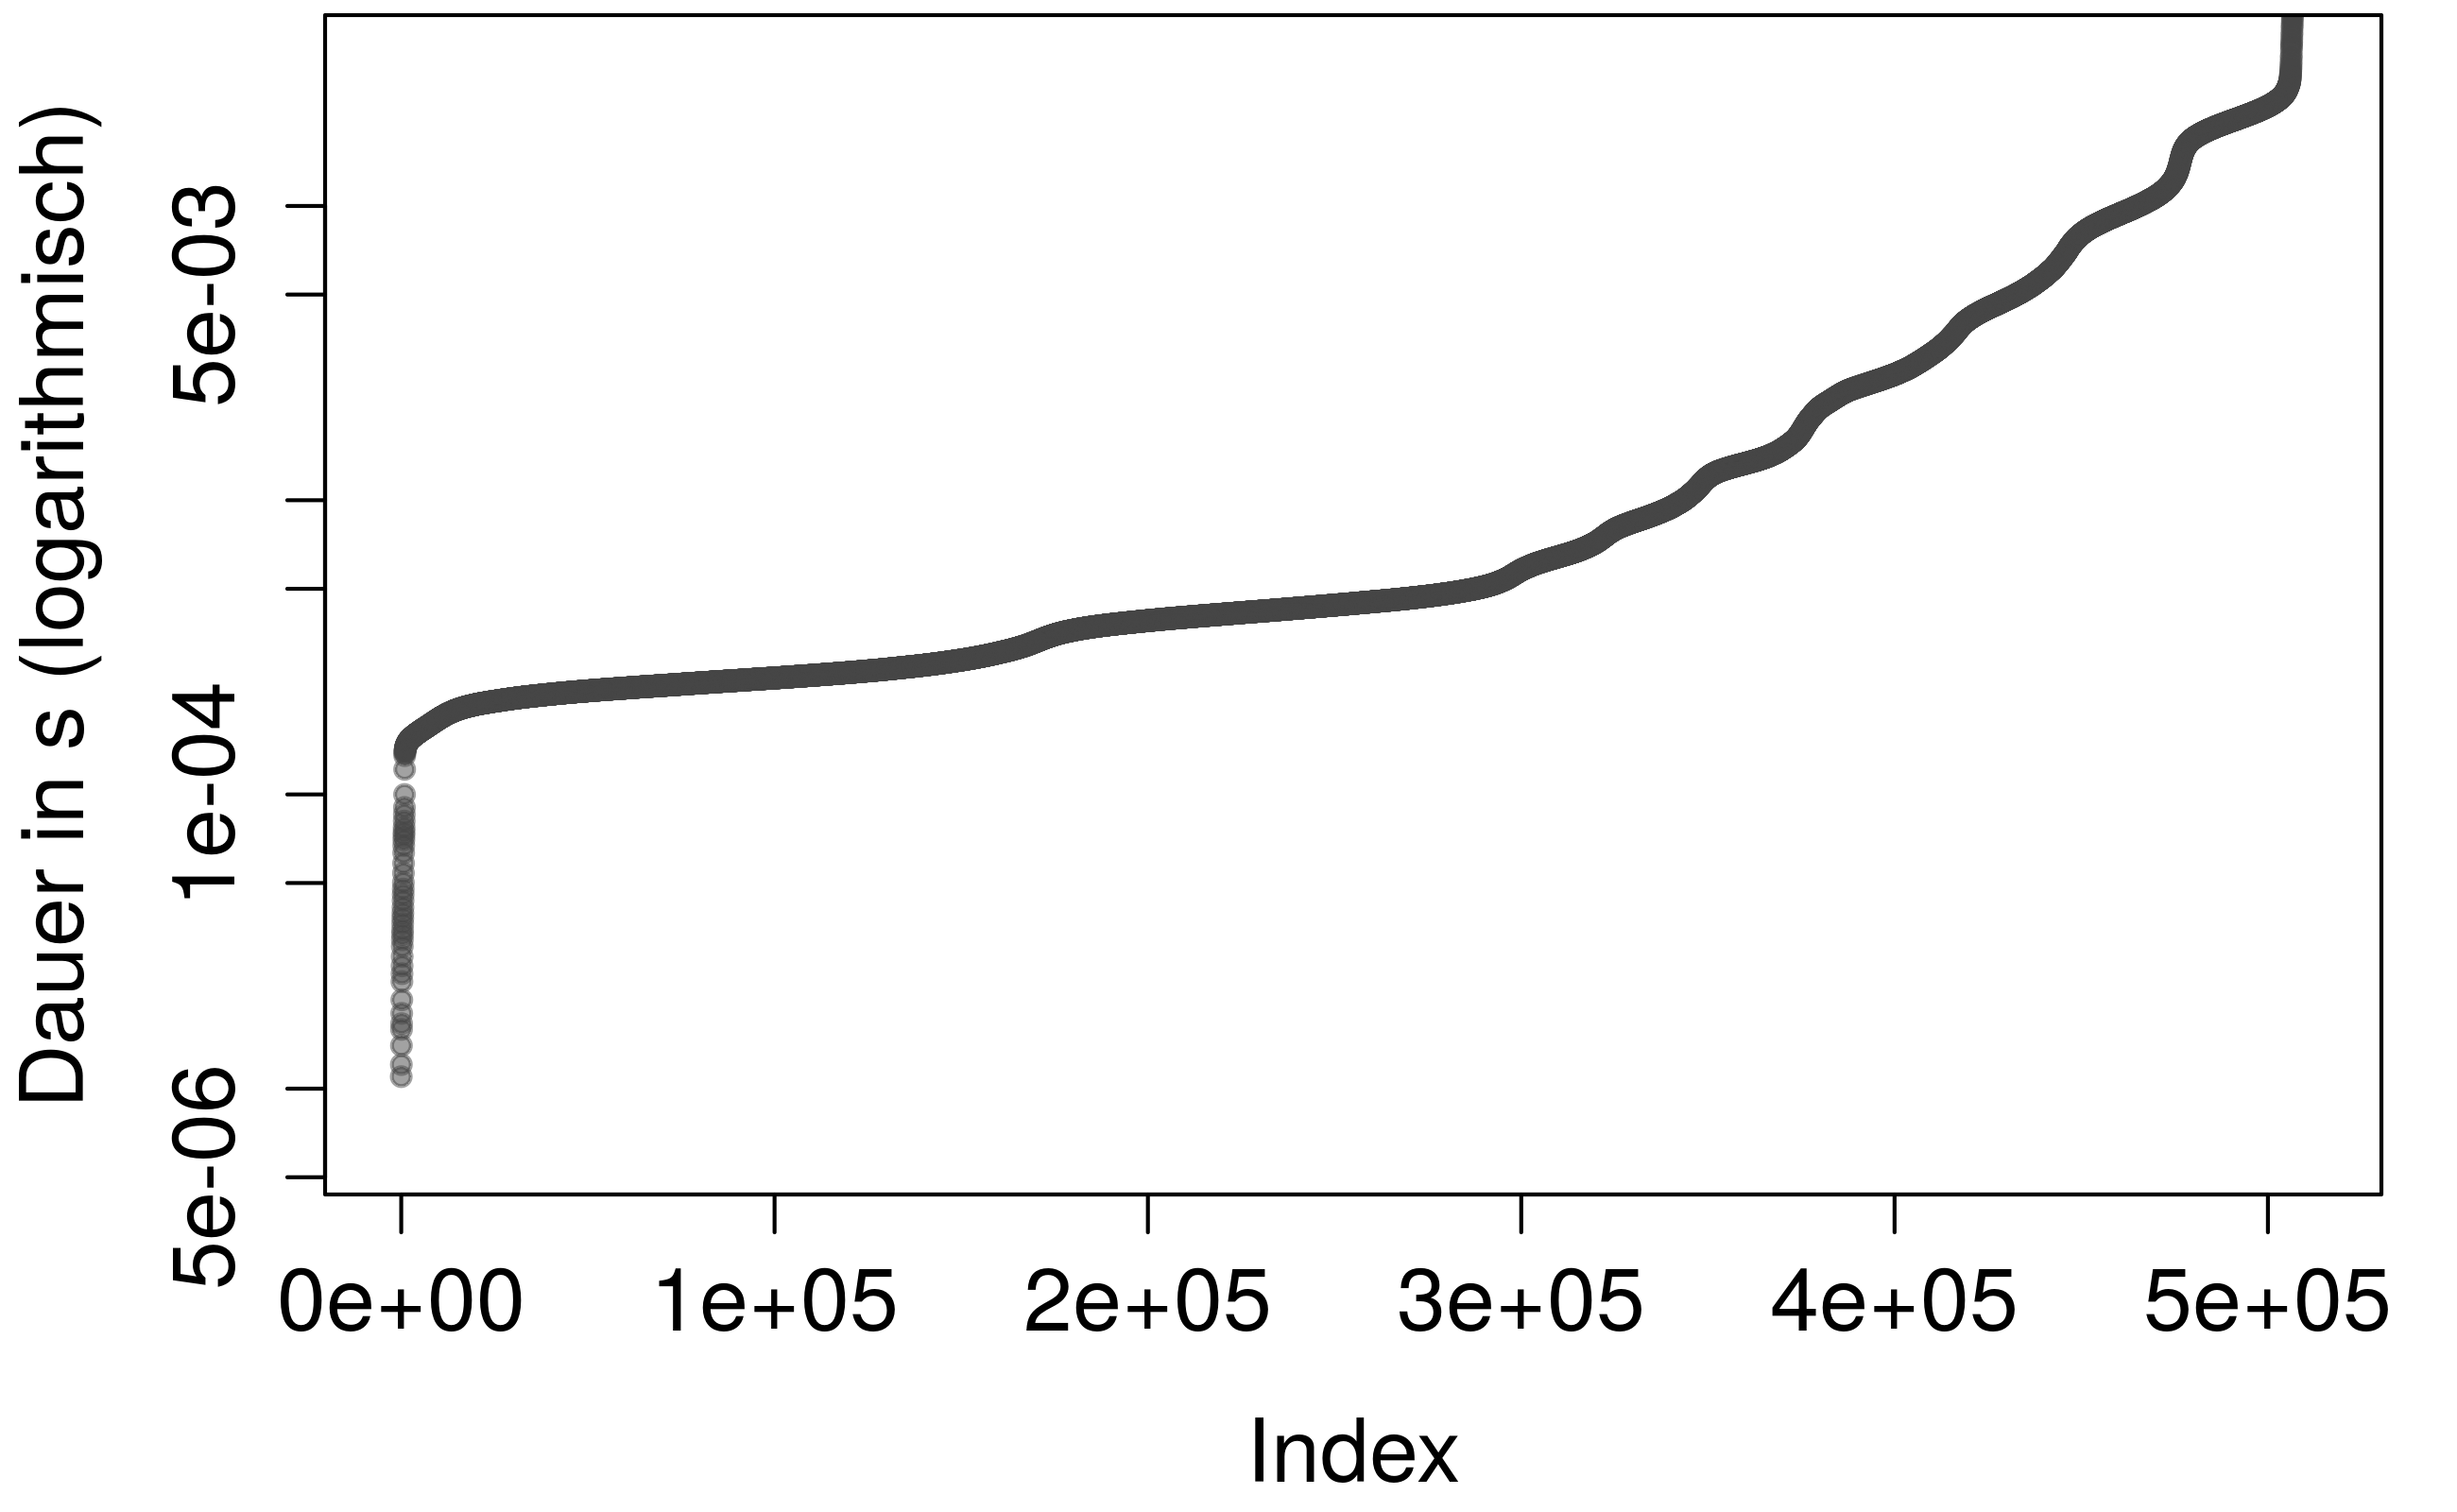
\includegraphics[width=.43\textwidth]{Bilder/Plots/exploration/plot_DurationSorted_write_rnd.png}
	}		
	\caption{Messungen der Laufzeiten sortiert dargestellt.}
	\label{Laufzeiten_Sortiert}
\end{figure} 

Als Ausreißer werden für alle Attribut-Sets die Messungen mit den $10\%$ kürzesten und längsten Laufzeiten behandelt. Die Verteilung der Ausreißer ist in \ref{fig:ausreisser} erkennen.
Bei den randomisierten Daten gibt es pro Attribut-Set nur ein bis drei Messungen. Daher führt diese Definition für Ausreißer auf dem Datensatz zu keinen sinnvollen Ergebnissen. 
Die Ausreißervorhersage wird dementsprechend im Folgenden nur auf dem sequentiellen Datensatz durchgeführt.
Dort befinden sich die Ausreißer gerade an den oberen und unteren Enden einer Stufe.

\begin{figure}
	\subfloat[Sequentiell lesend]{
		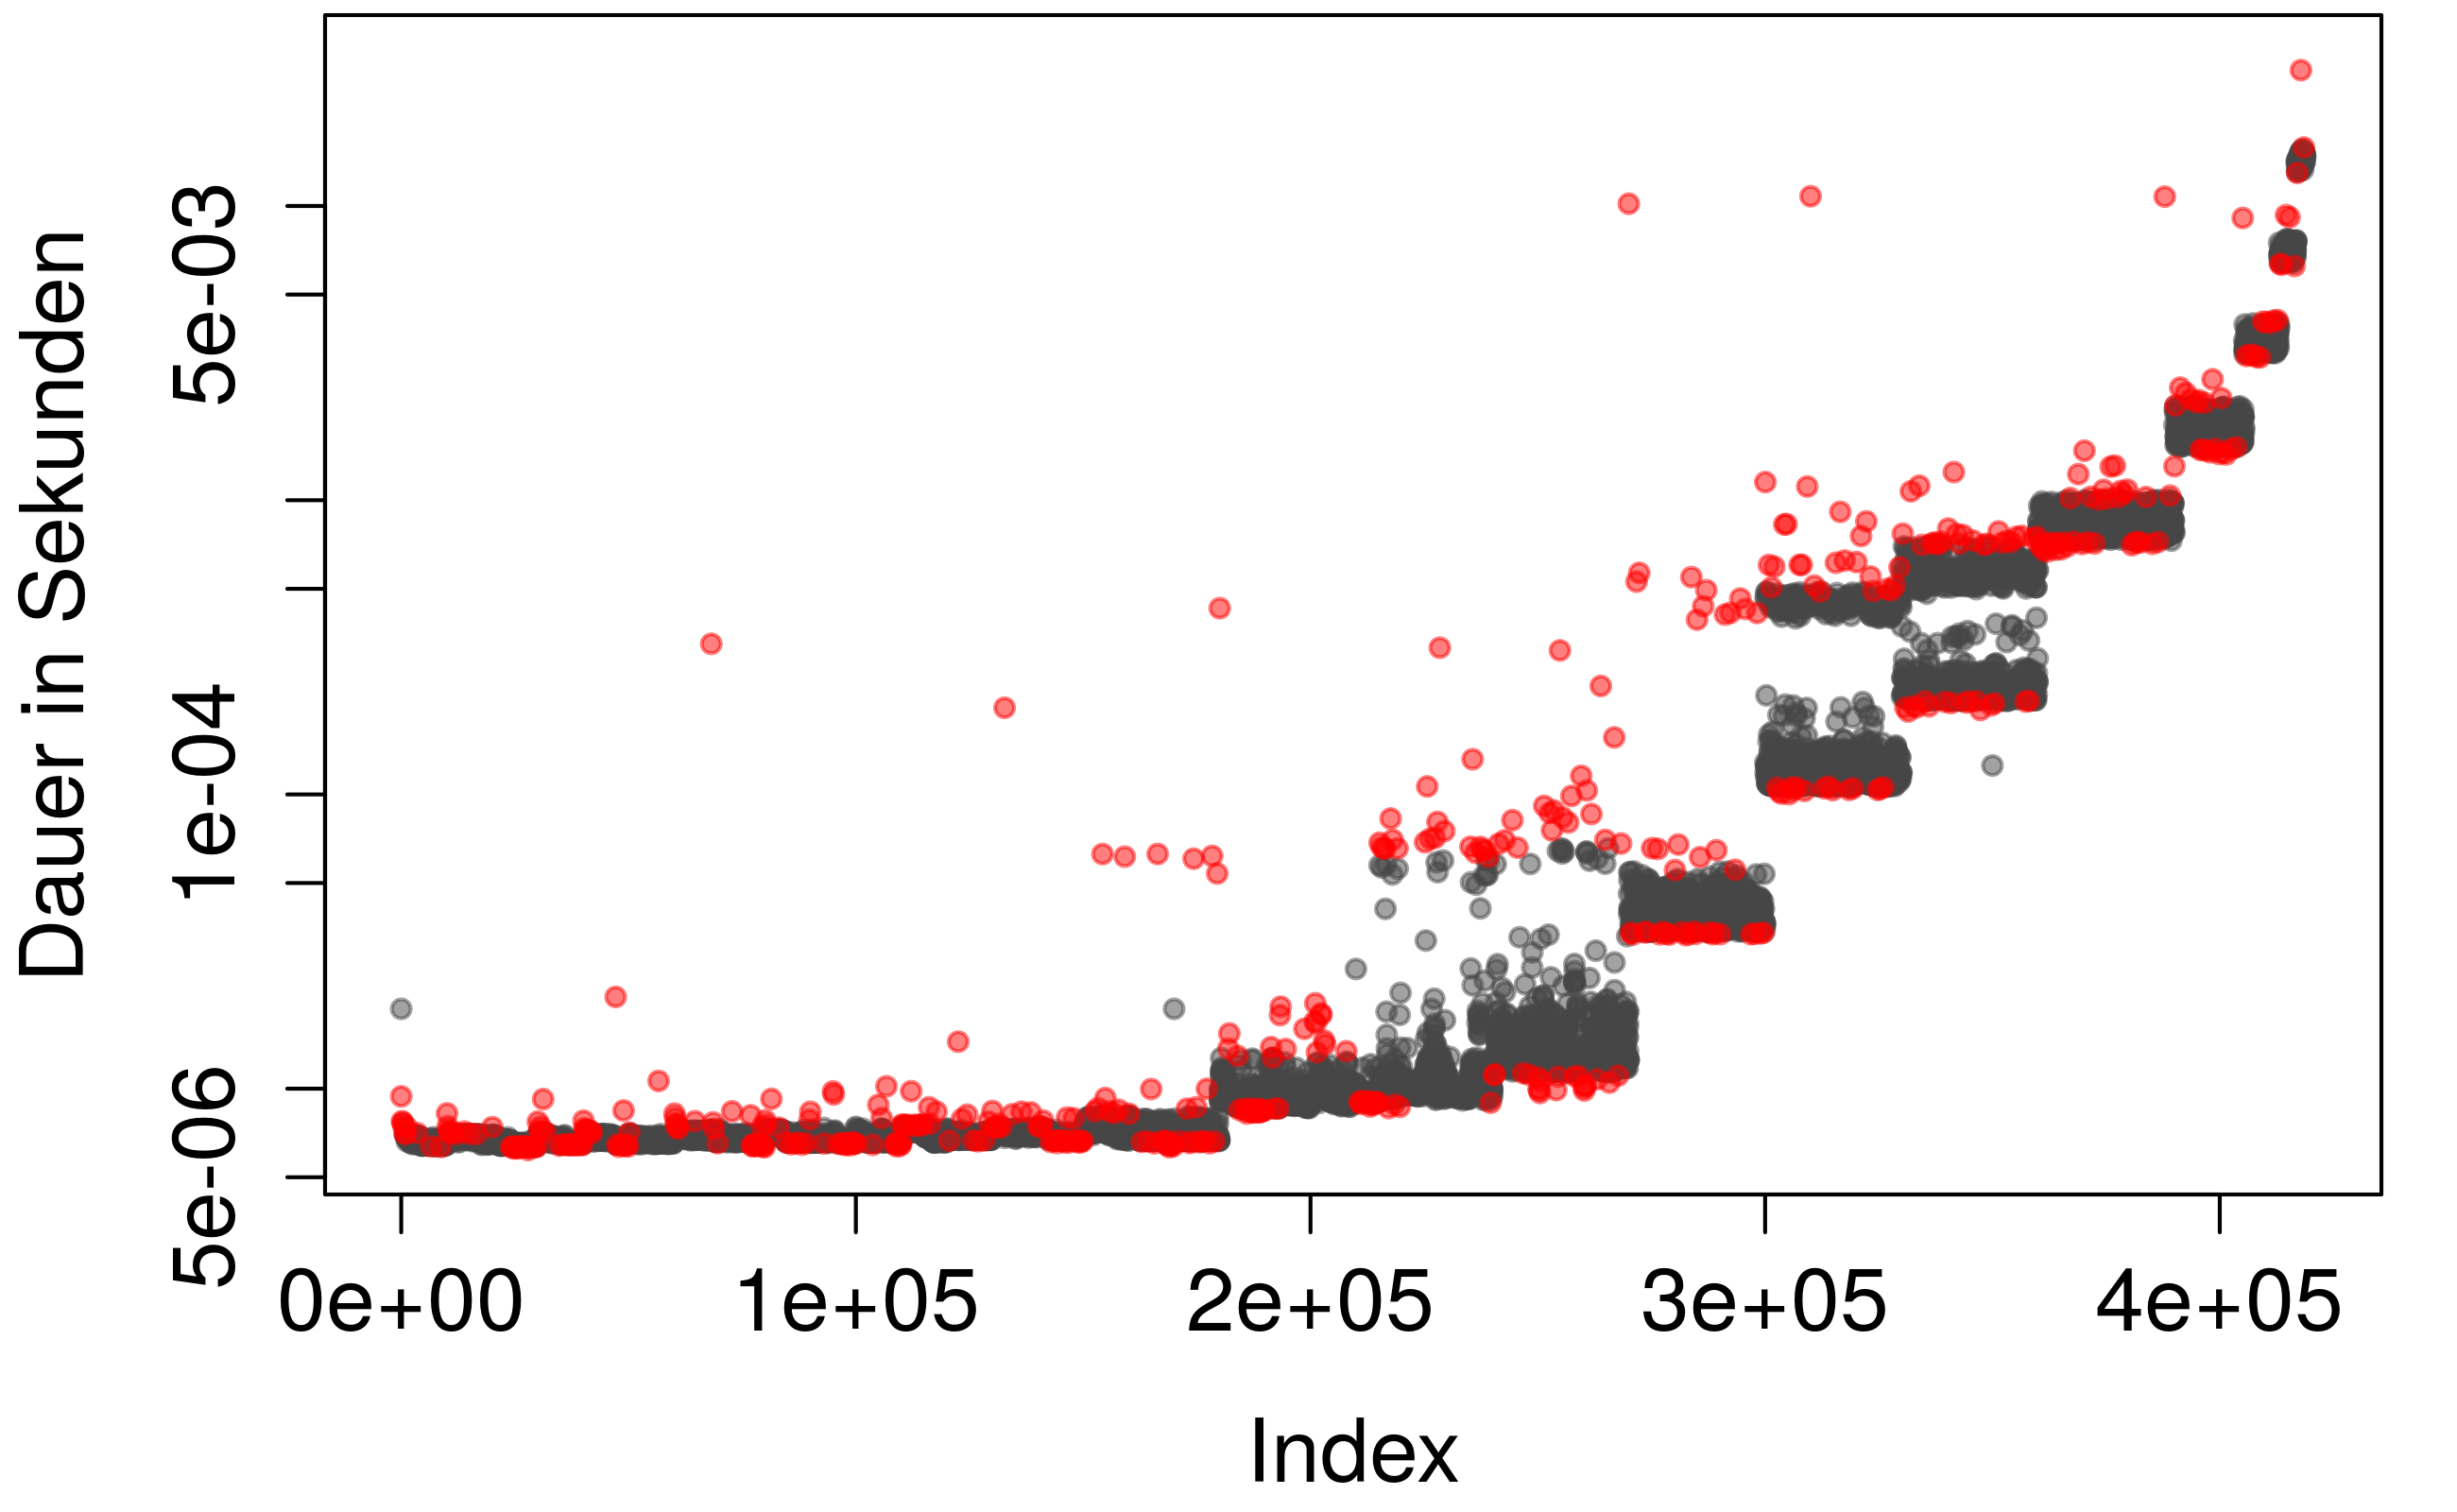
\includegraphics[width=.43\textwidth]{Bilder/Plots/exploration/plot_outlier_read_seq.png}
	}
	\hfill
	\subfloat[Sequentiell schreibend]{
		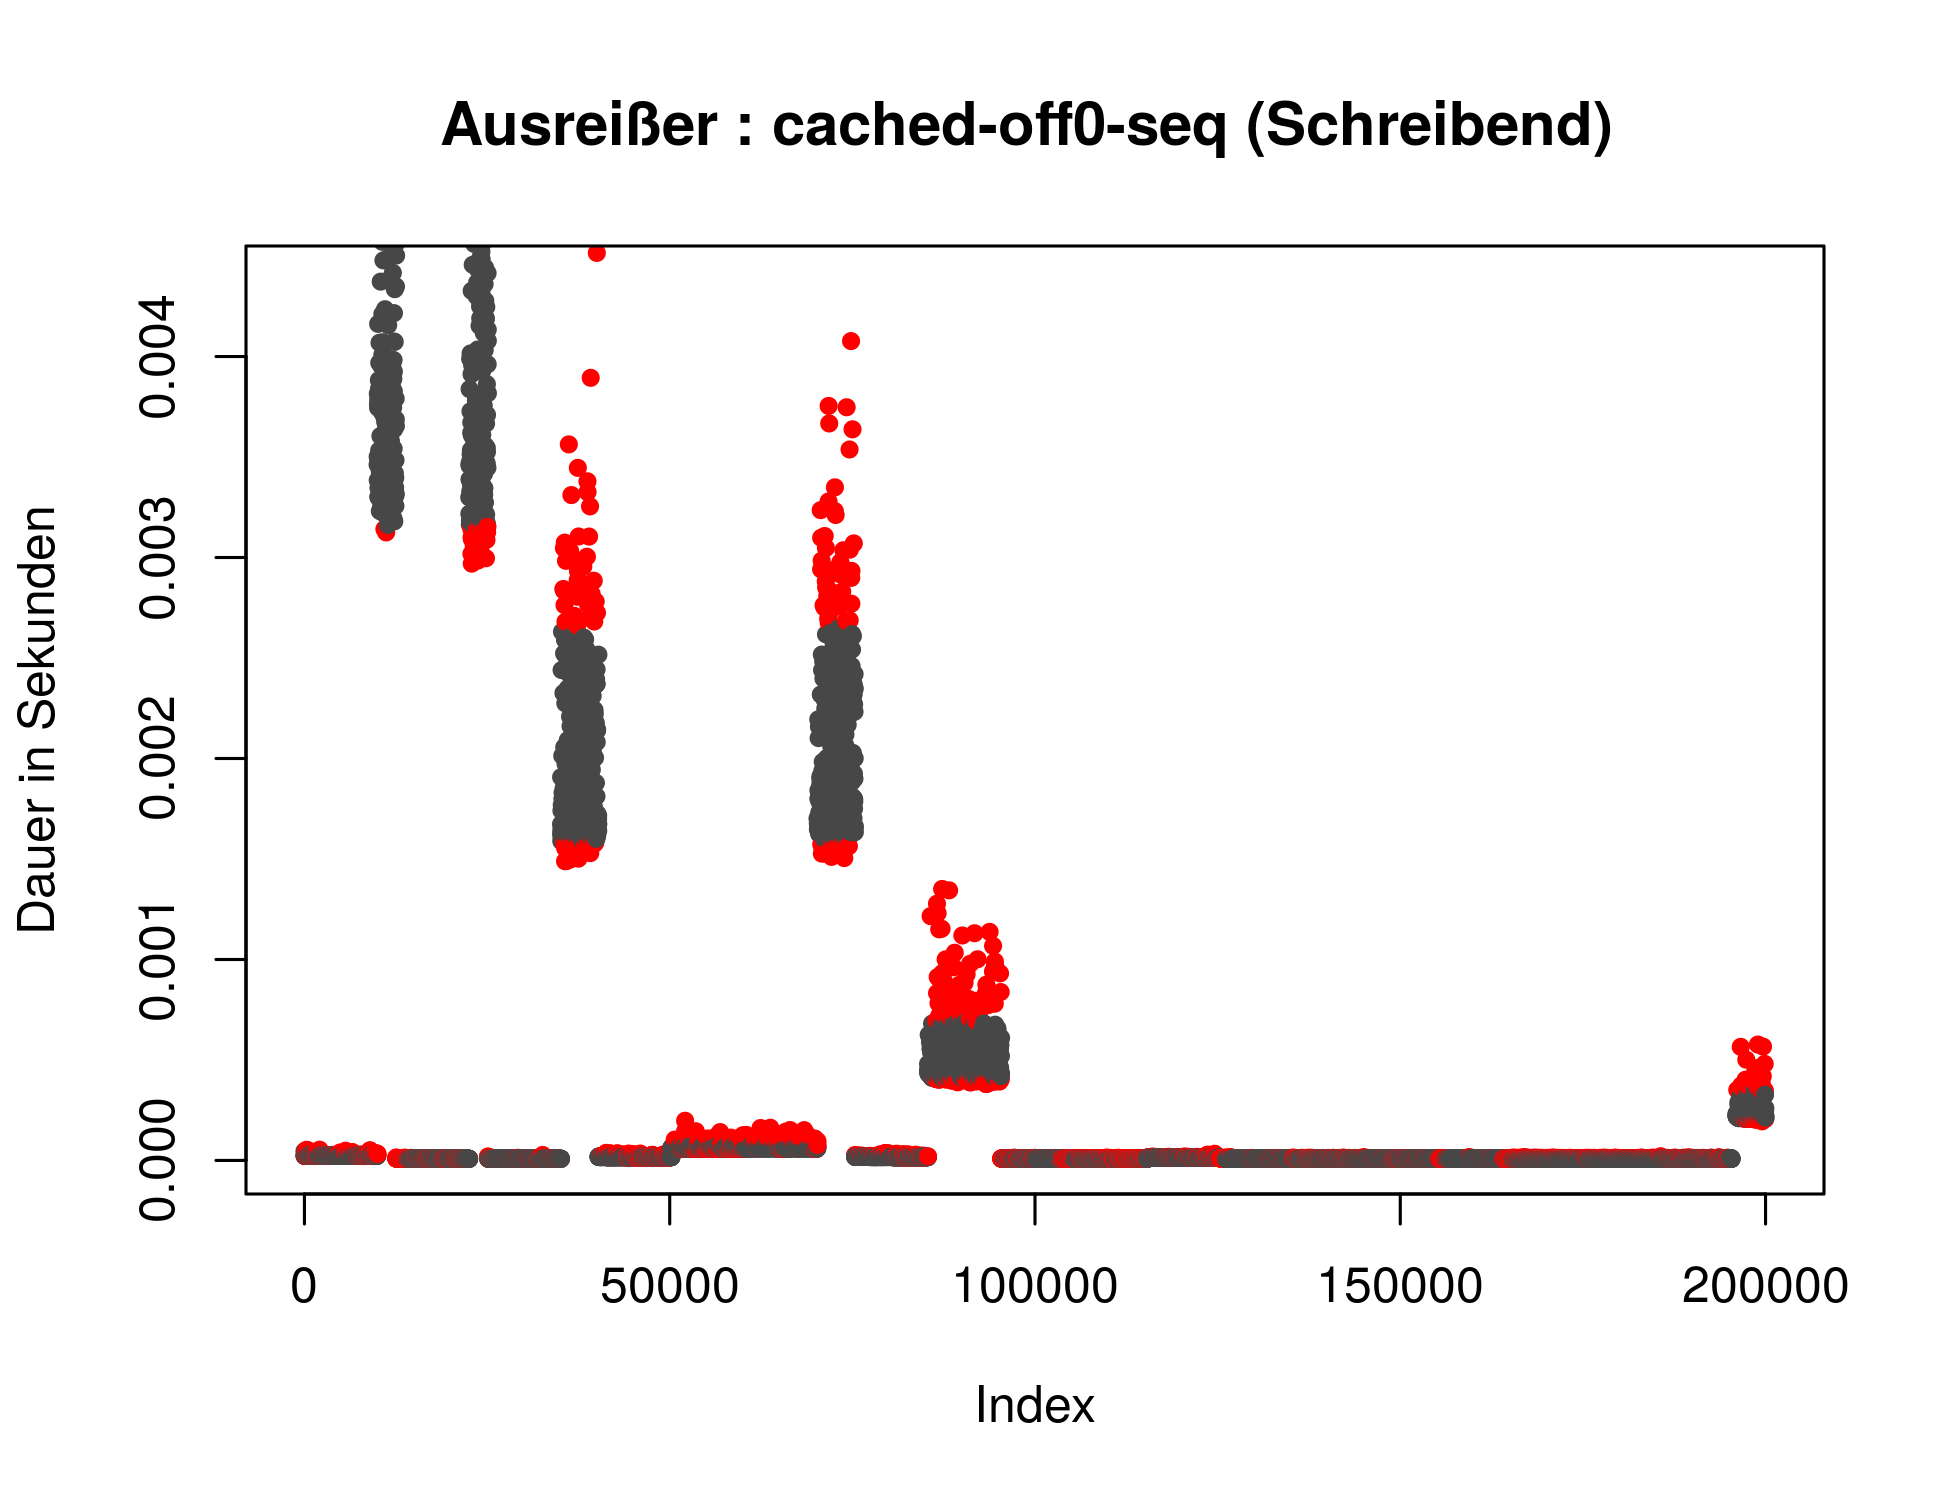
\includegraphics[width=.43\textwidth]{Bilder/Plots/exploration/plot_outlier_write_seq.png}
	}	
	\caption{Ausreißer sind in rot dargstellt, sie überdecken die grauen Punkte}
	\label{fig:ausreisser}
\end{figure} 

Um die unterschiedlichen Laufzeiten innerhalb einer Zugriffsgröße zu untersuchen, habe ich in Abbildung \ref{fig:groesse1} bis \ref{fig:groesse2097152} für die Größen 1B, 16KiB und 2MiB alle Messungen betrachtet.
In den Graphen ist gut zu erkennen, dass die Varianz der Laufzeiten im sequentiellen Fall wesentlich geringer ausfällt, als bei den randomisierten Messungen.
Teilweise lassen sich die verschiedenen Messreihen (eine Messreihe umfasst 10000 Messungen, außer im 2MiB Fall, dort sind es 5000) am Muster der Zugriffszeiten voneinander unterscheiden.
So ist eine Verschiebung des Musters bei \ref{fig:groesse16384} c) nach 10000 und 20000 Messungen deutlich zu erkennen.
Abhängig vom Systemzustand konnten die Anfragen also im Mittel unterschiedlich schnell bearbeitet werden.
In einigen Bildern lassen sich auch kurzzeitige Spitzen zwischen den Messreihen feststellen.
Beim sequentiell lesenden Fall für ein Byte dauern die ersten Messungen jeweils wesentlich länger, bis sich ein niedriger Wert eingependelt hat. Hier scheinen nach einigen Zugriffen die Read-Ahead Caching-Strategie zu greifen, die angefragten Daten befinden sich dann bereits im Cache. Dies macht auch Sinn, da der sequentielle Zugriff sehr gut vorhersagbar ist.
Für die randomisierten Datensätze ist ein solches Verhalten nicht möglich und kann auch in keiner Abbildung erkannt werden.
Ein interessantes Verhalten kann in \ref{fig:groesse16384} a) beobachtet werden.
Zu Beginn jeder Messerreihe werden die ersten E/A-Zugriffe zuverlässig sehr schnell ausgeführt, dann steigt die mittlere Zugriffszeit rapide an und oszilliert stark.
Möglicherweise wird in diesem Fall solange der Arbeitsspeicher aufgefüllt, bis der Platz nicht mehr ausreicht und aufwendigere Speicherverwaltungen Platz für die neuen Daten im Speicher schaffen müssen.

\begin{figure}
	\subfloat[Sequentiell lesend]{
		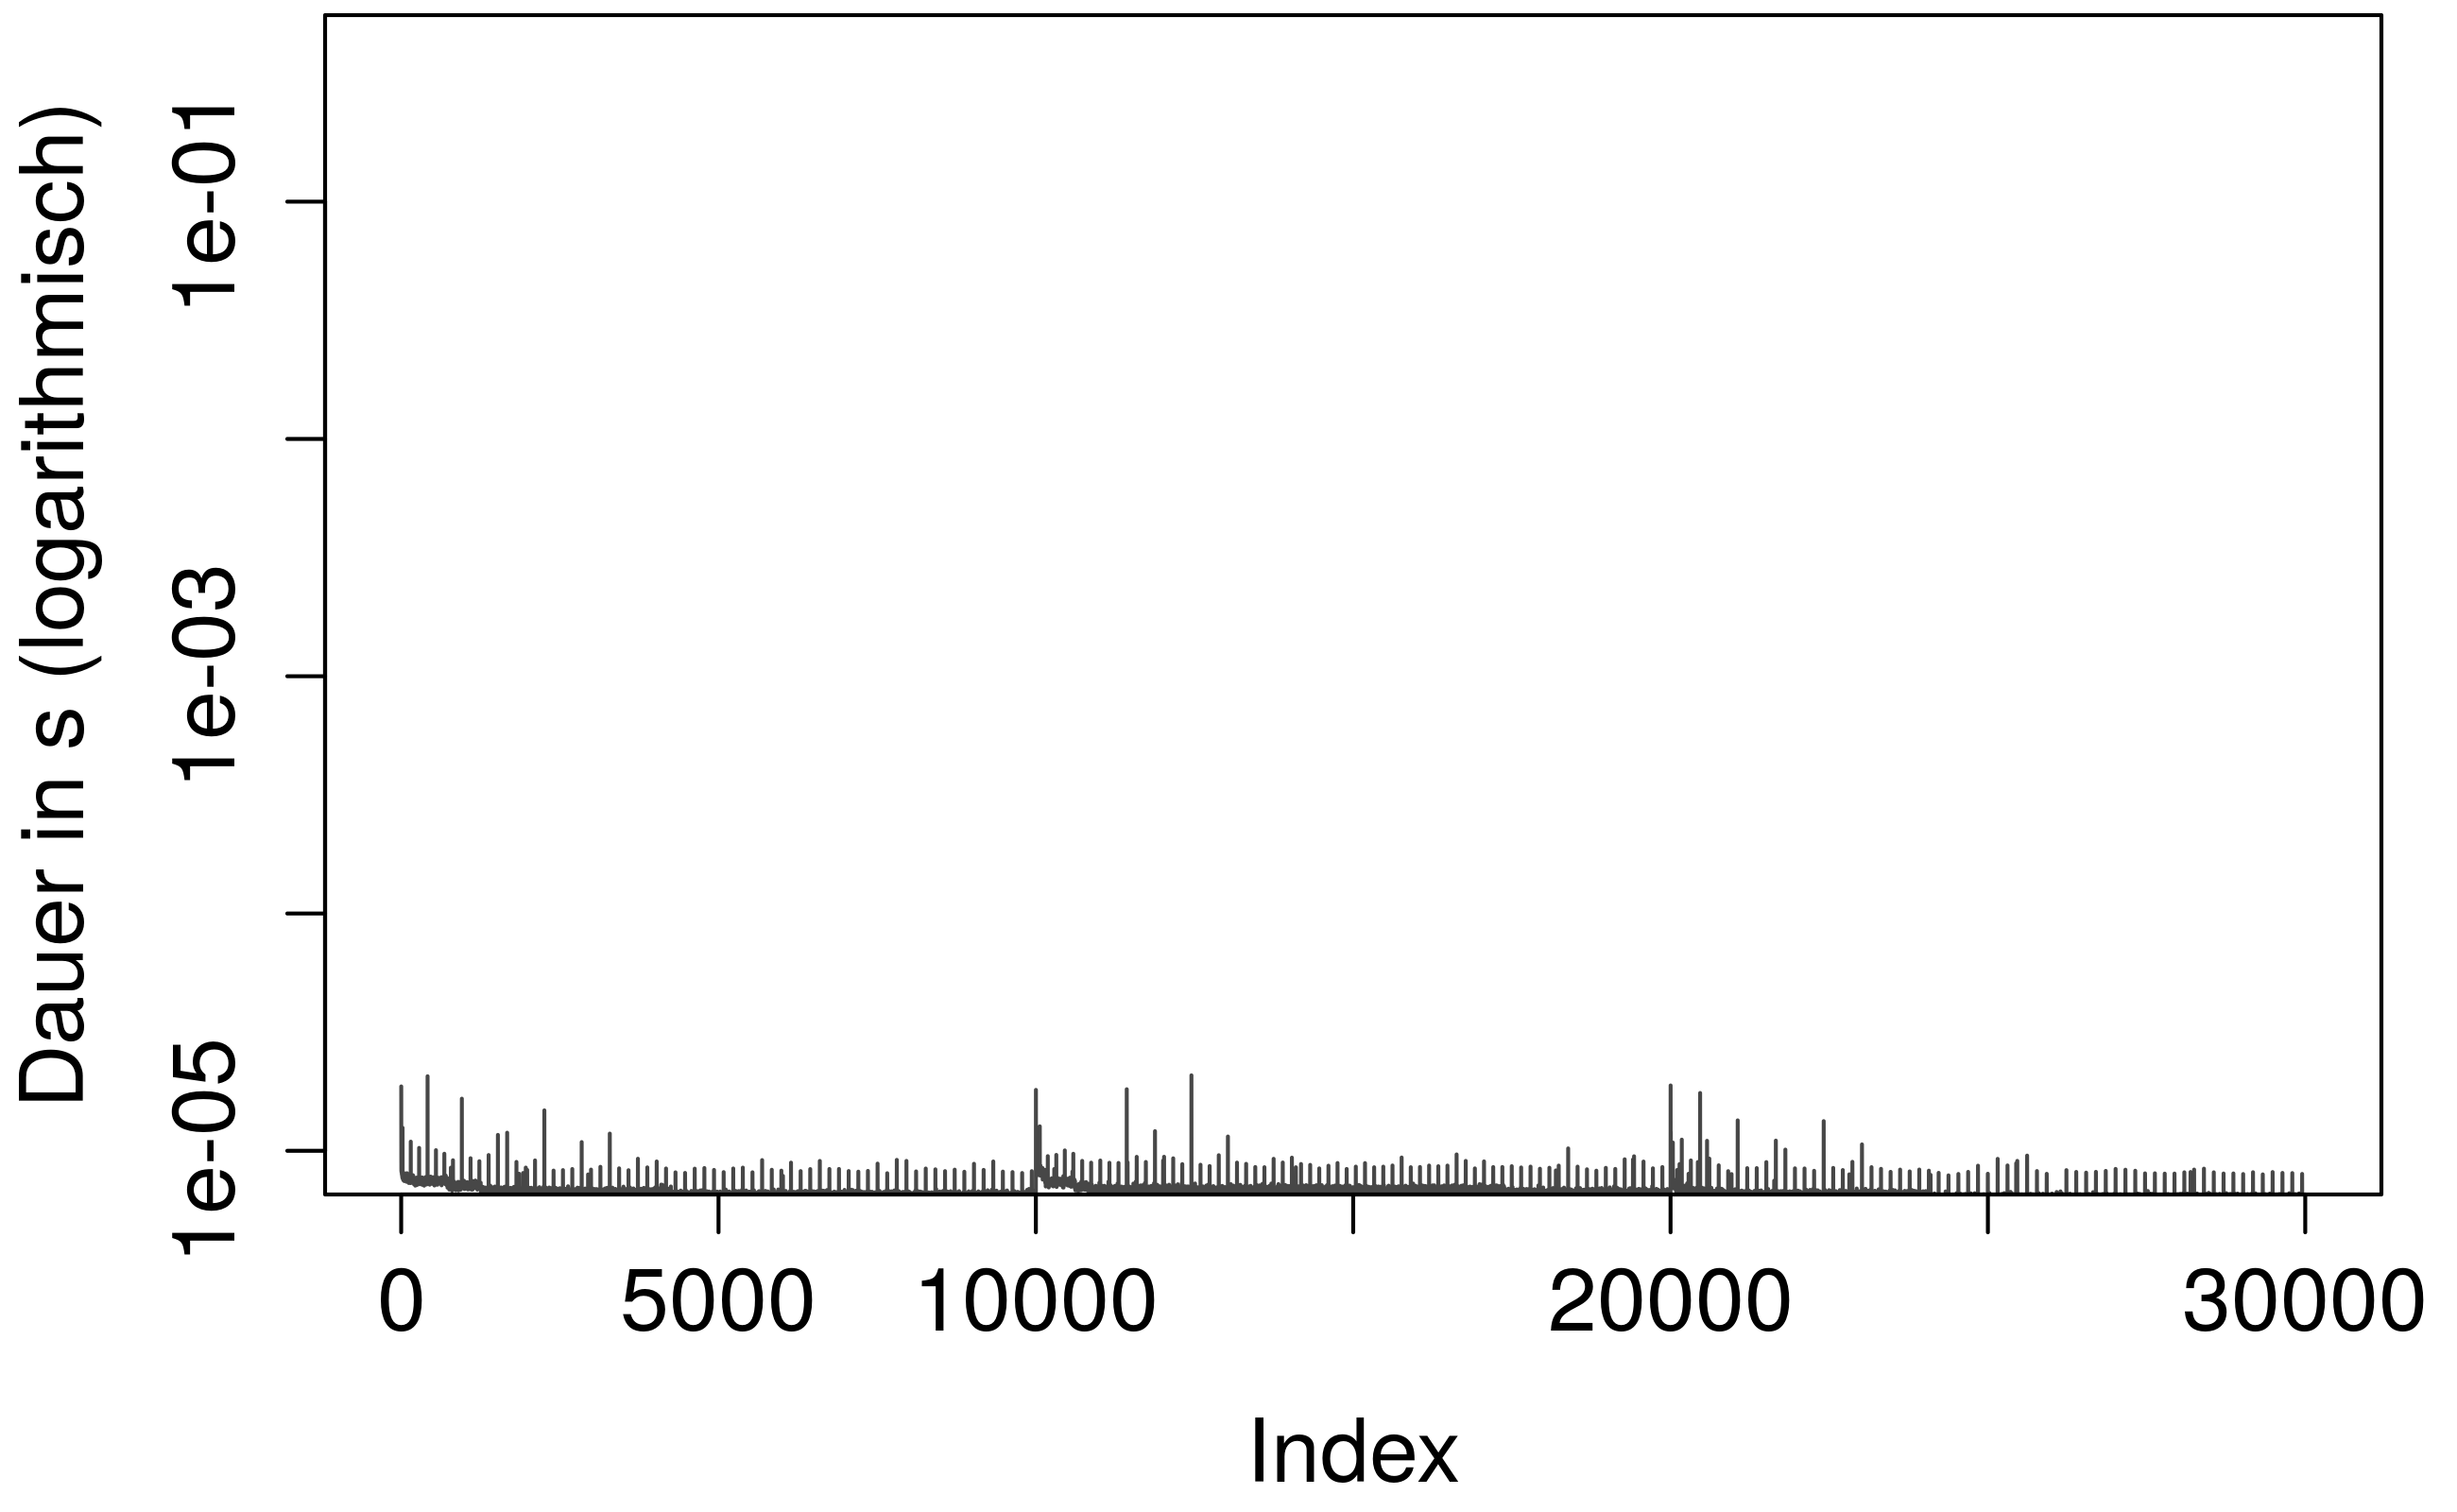
\includegraphics[width=.43\textwidth]{Bilder/Plots/exploration/plot_Size1_read_seq.png}
	}
	\hfill
	\subfloat[Sequentiell schreibend]{
		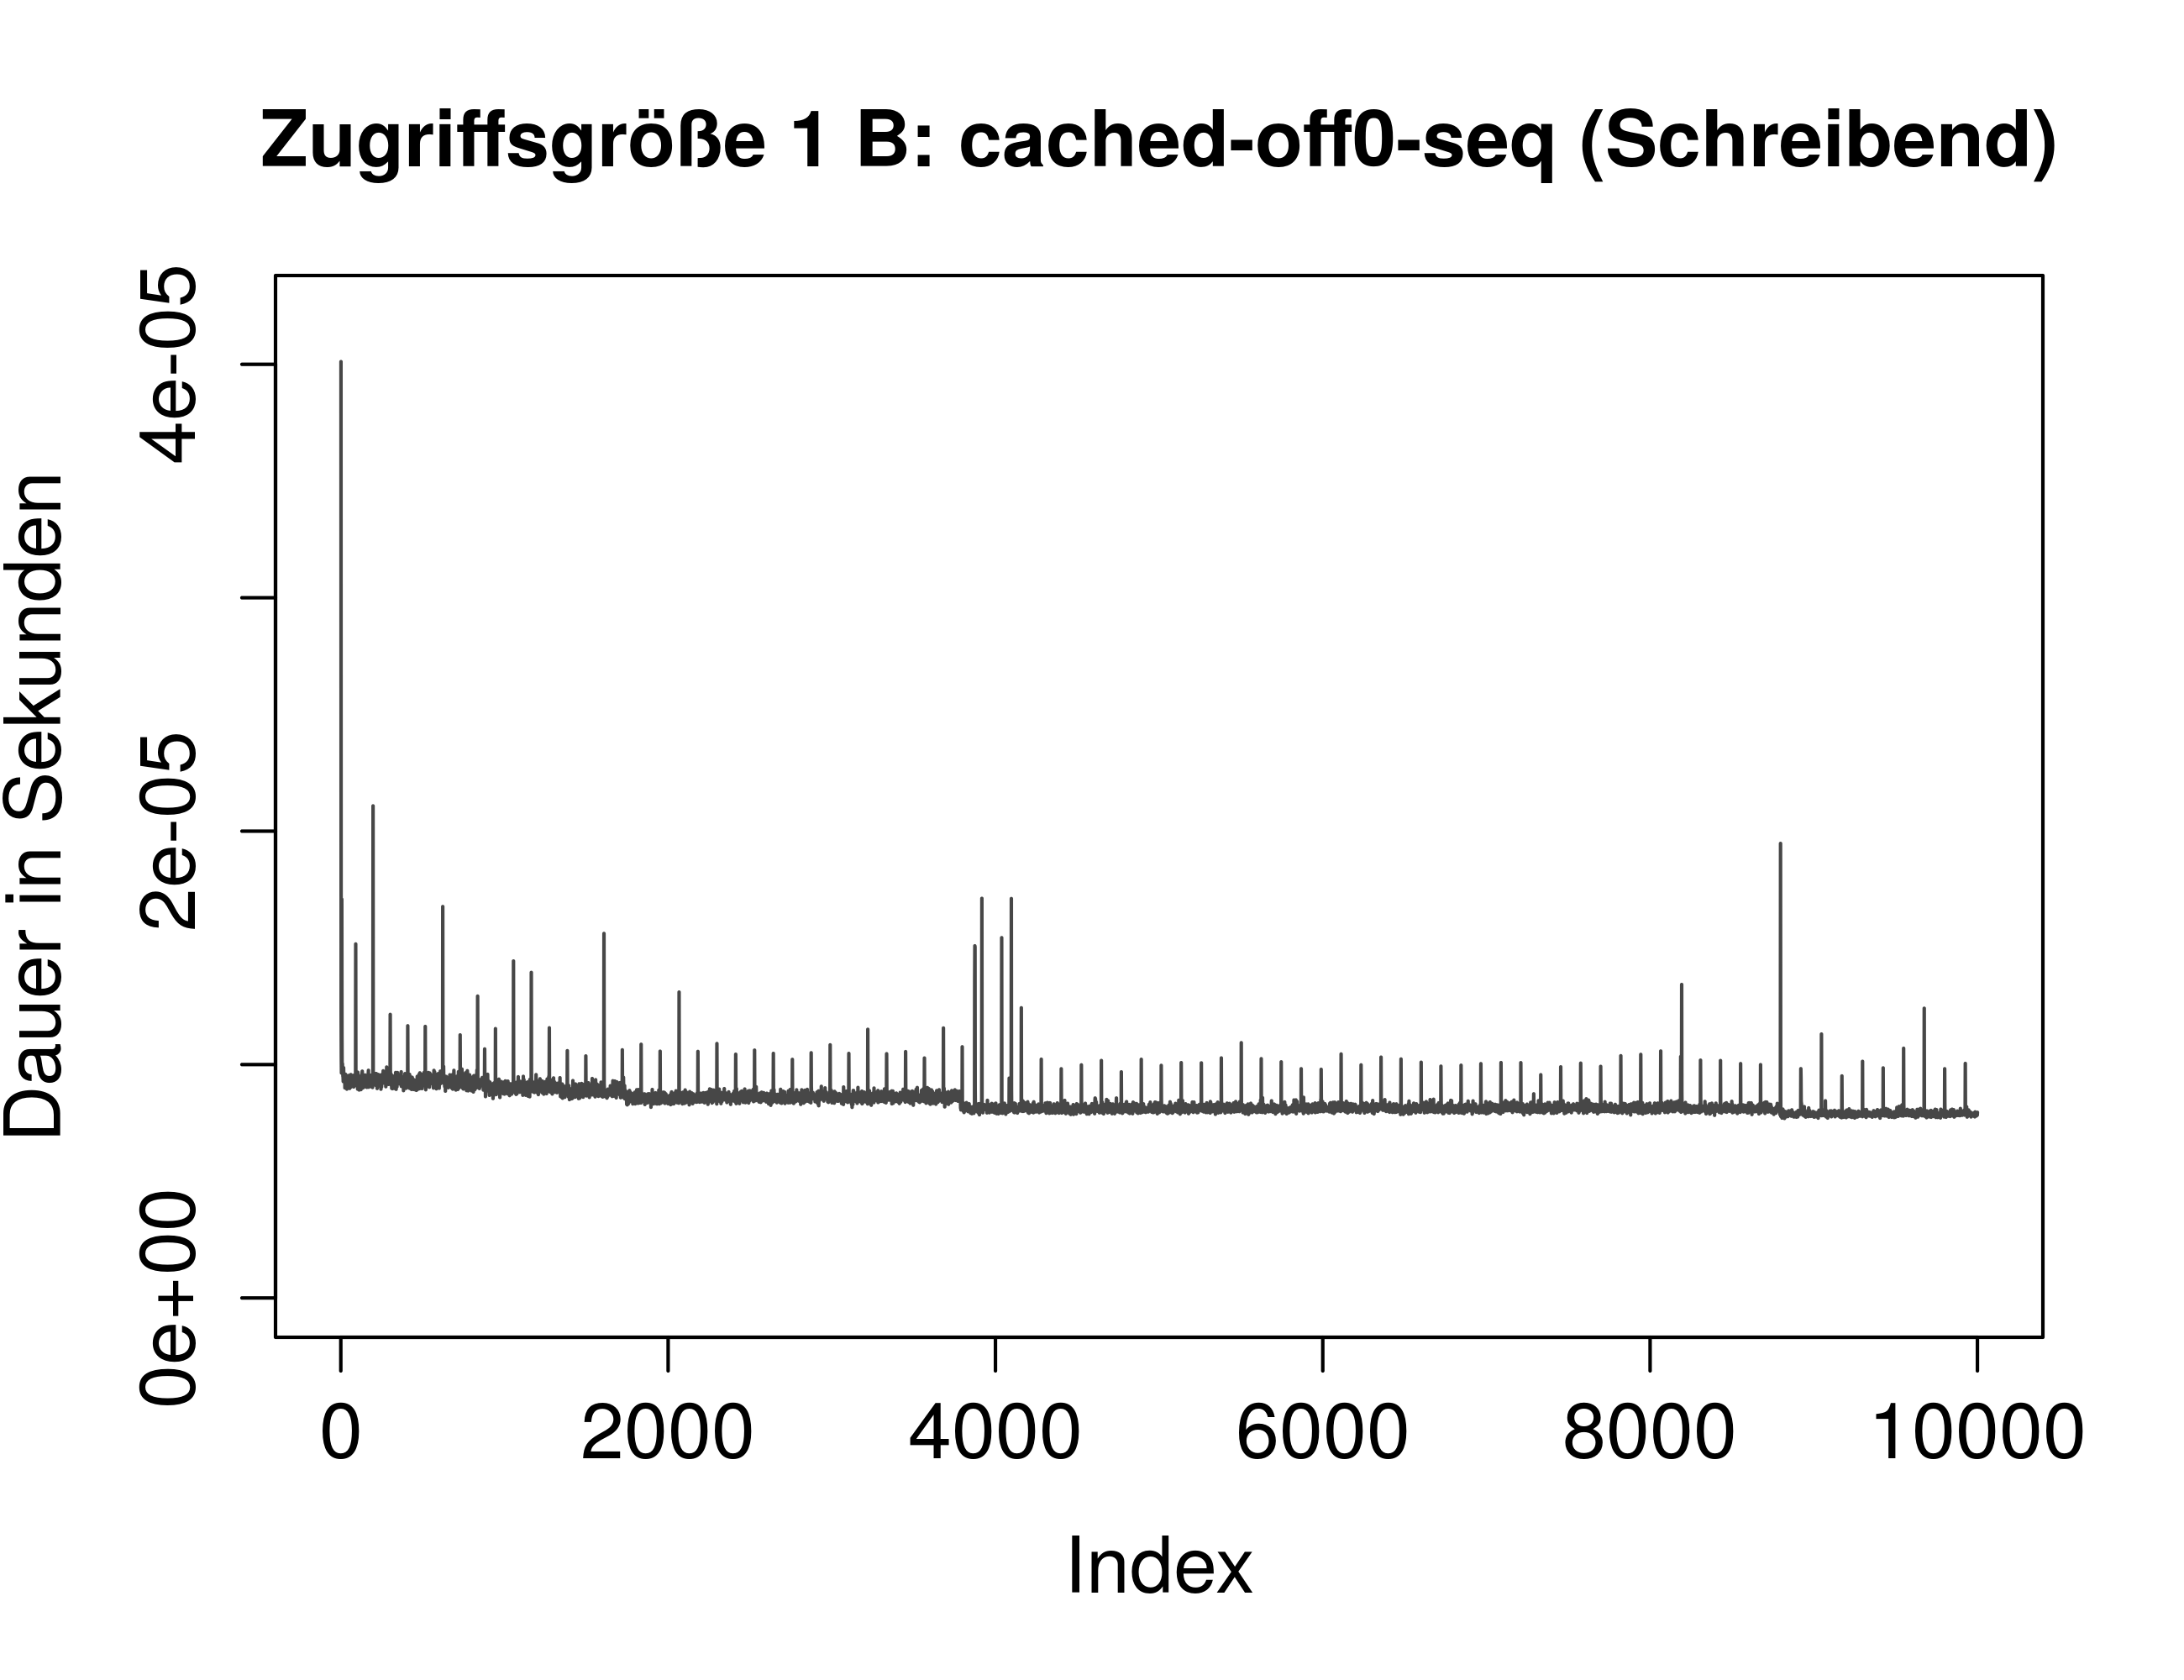
\includegraphics[width=.43\textwidth]{Bilder/Plots/exploration/plot_Size1_write_seq.png}
	}\\
	\subfloat[Randomisiert lesend]{
		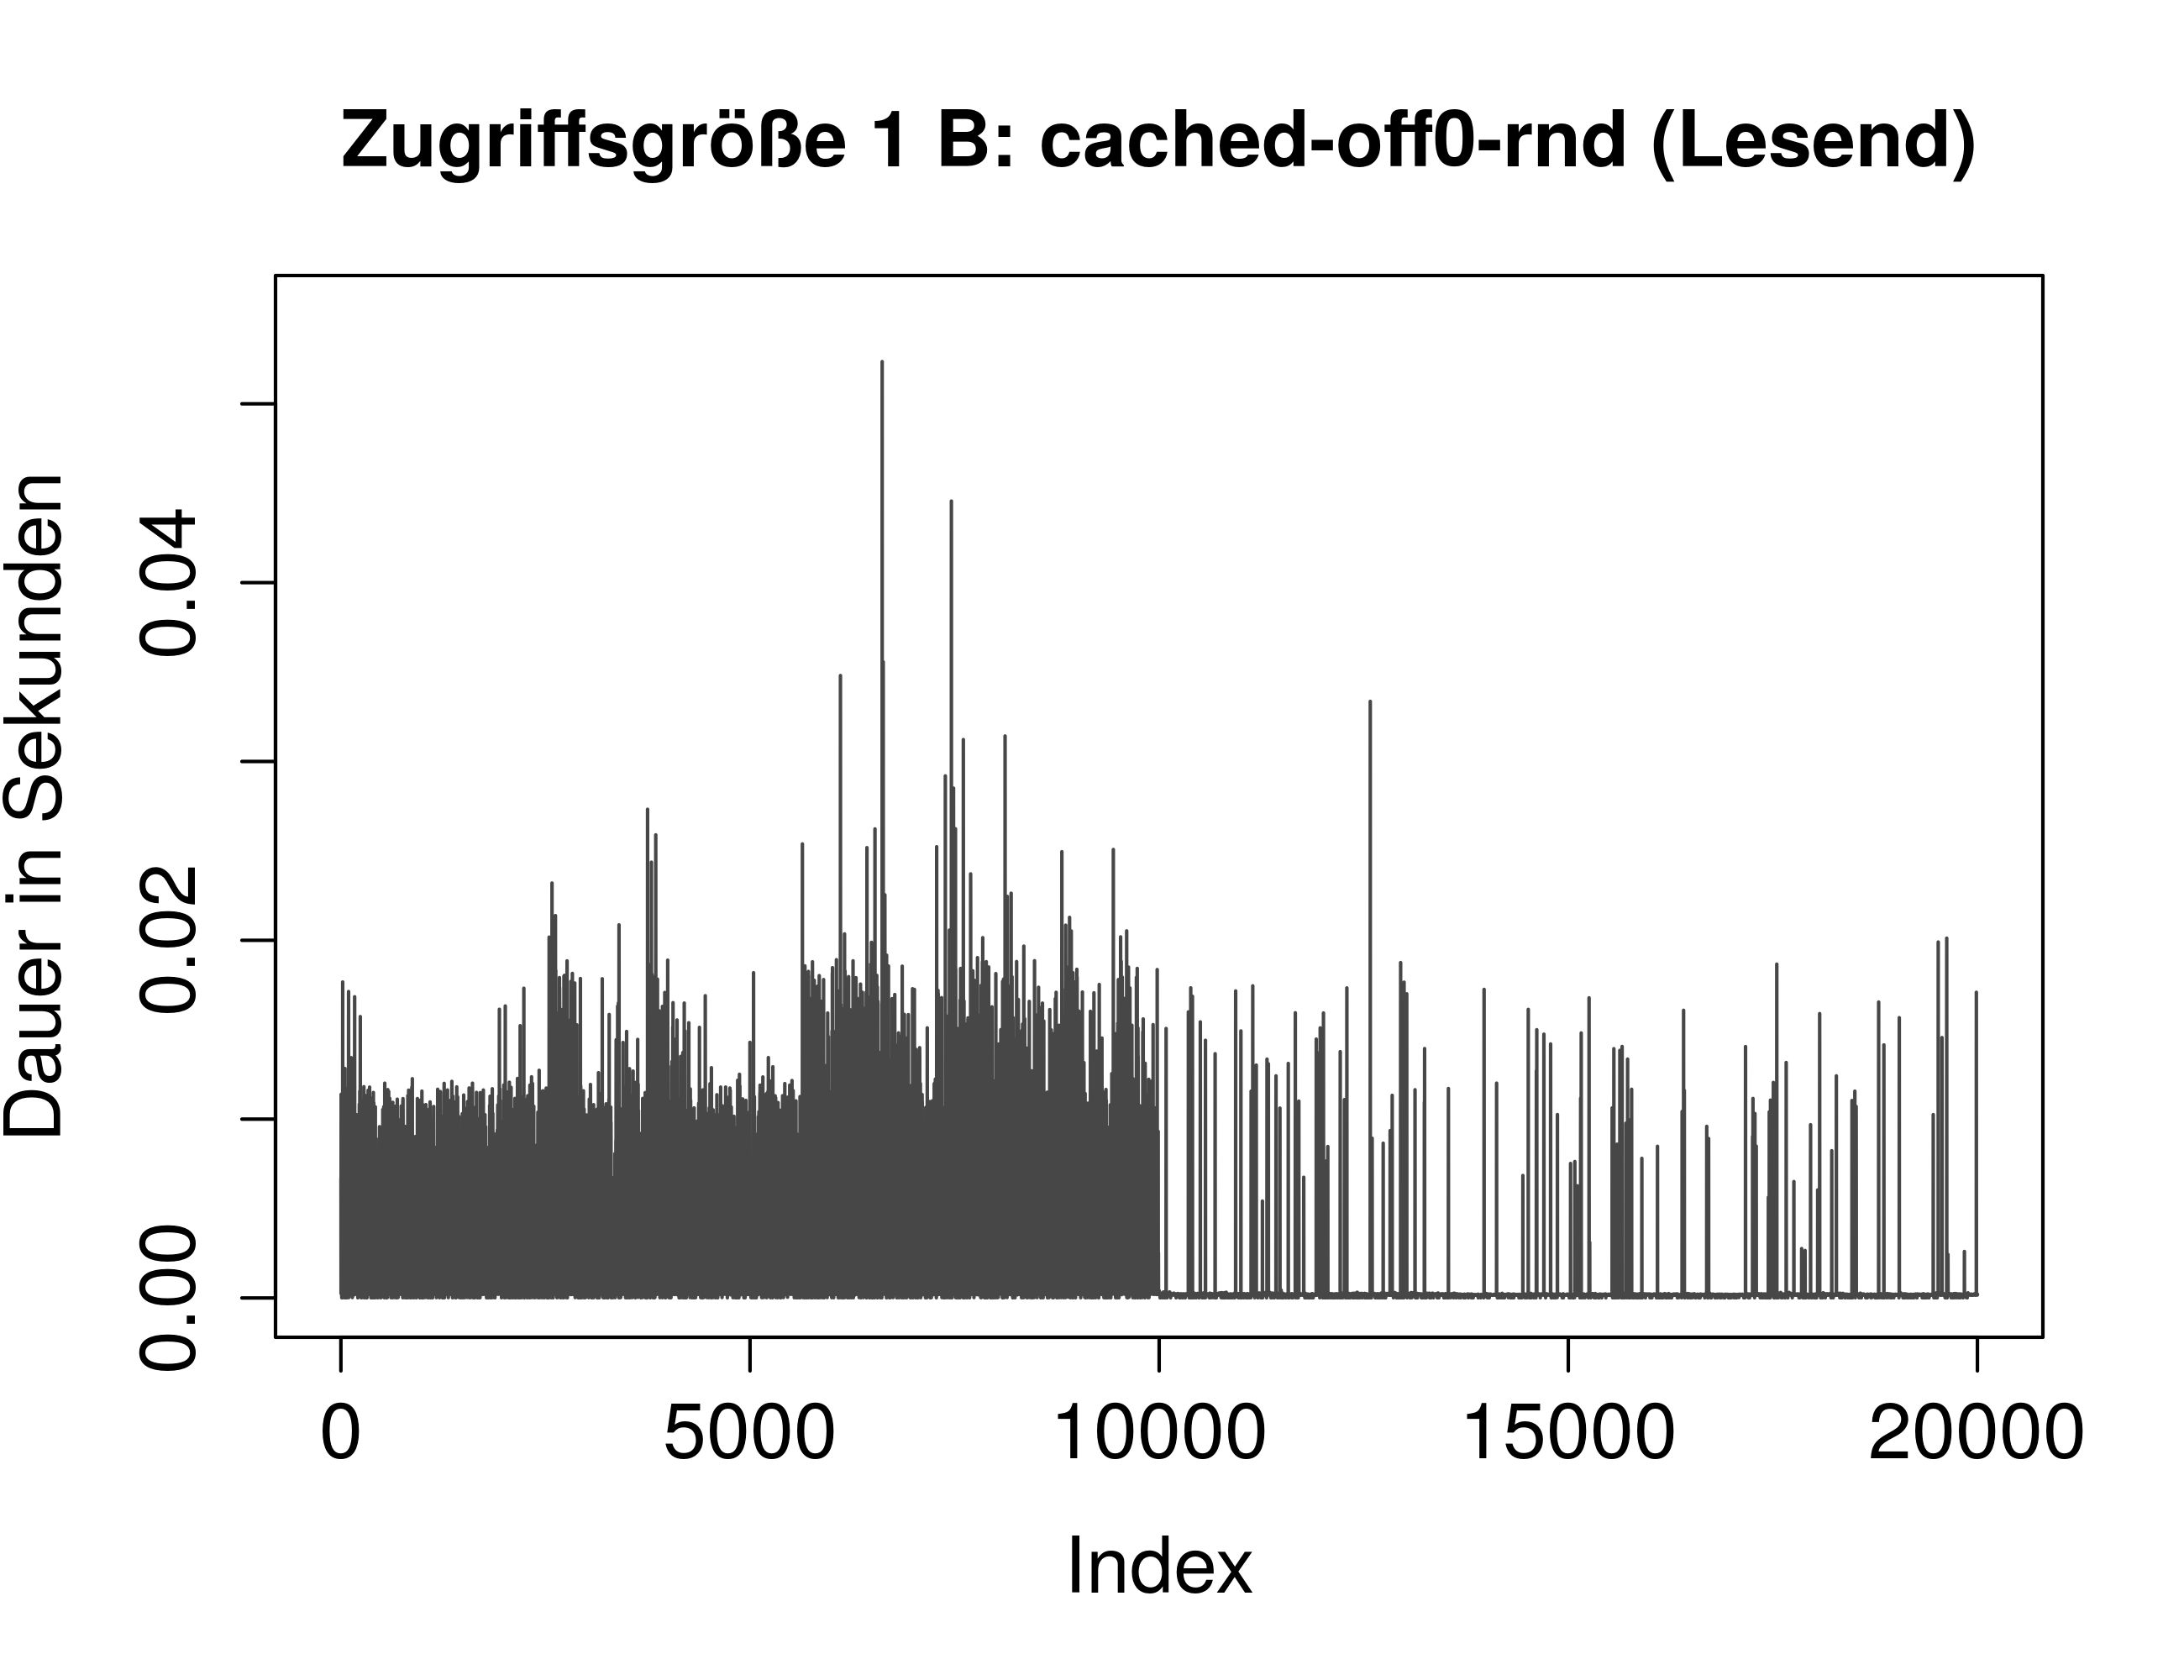
\includegraphics[width=.43\textwidth]{Bilder/Plots/exploration/plot_Size1_read_rnd.png}
	}
	\hfill
	\subfloat[Randomisiert schreibend]{
		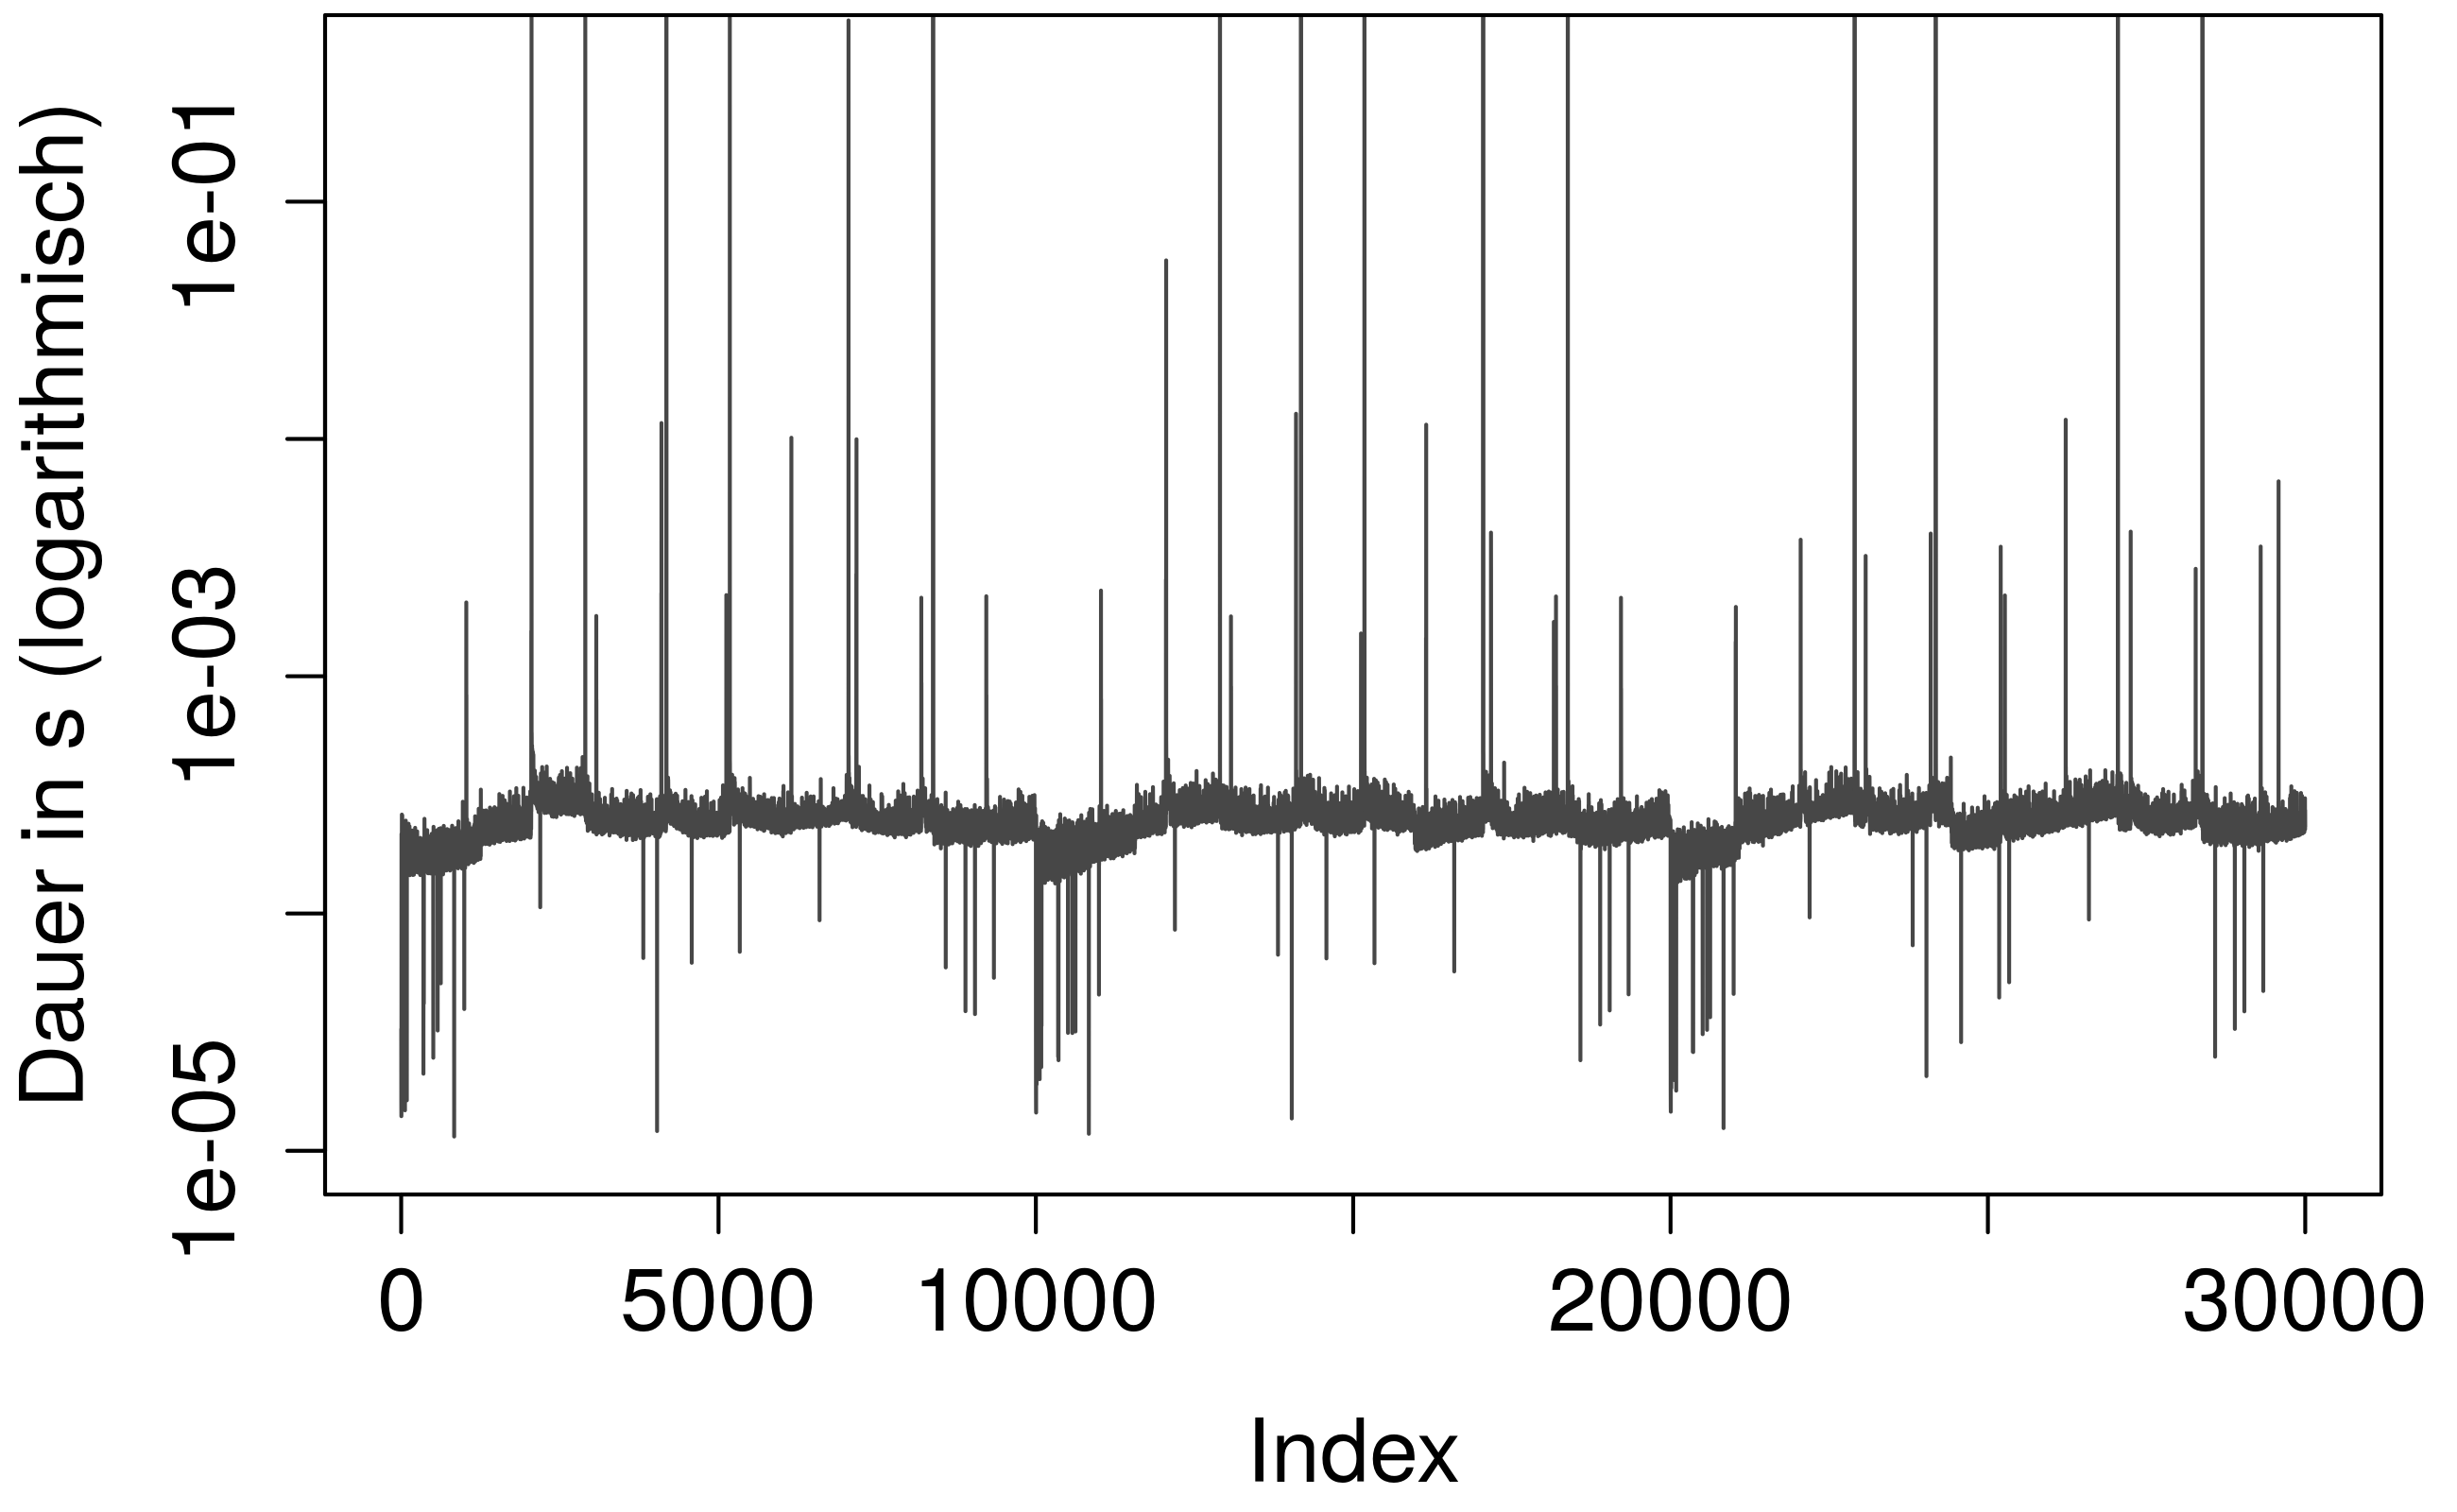
\includegraphics[width=.43\textwidth]{Bilder/Plots/exploration/plot_Size1_write_rnd.png}
	}		
	\caption{Detailbetrachtung aller Messungen mit Zugriffsgröße 1B}
	\label{fig:groesse1}
\end{figure}
\begin{figure}
	\subfloat[Sequentiell lesend]{
		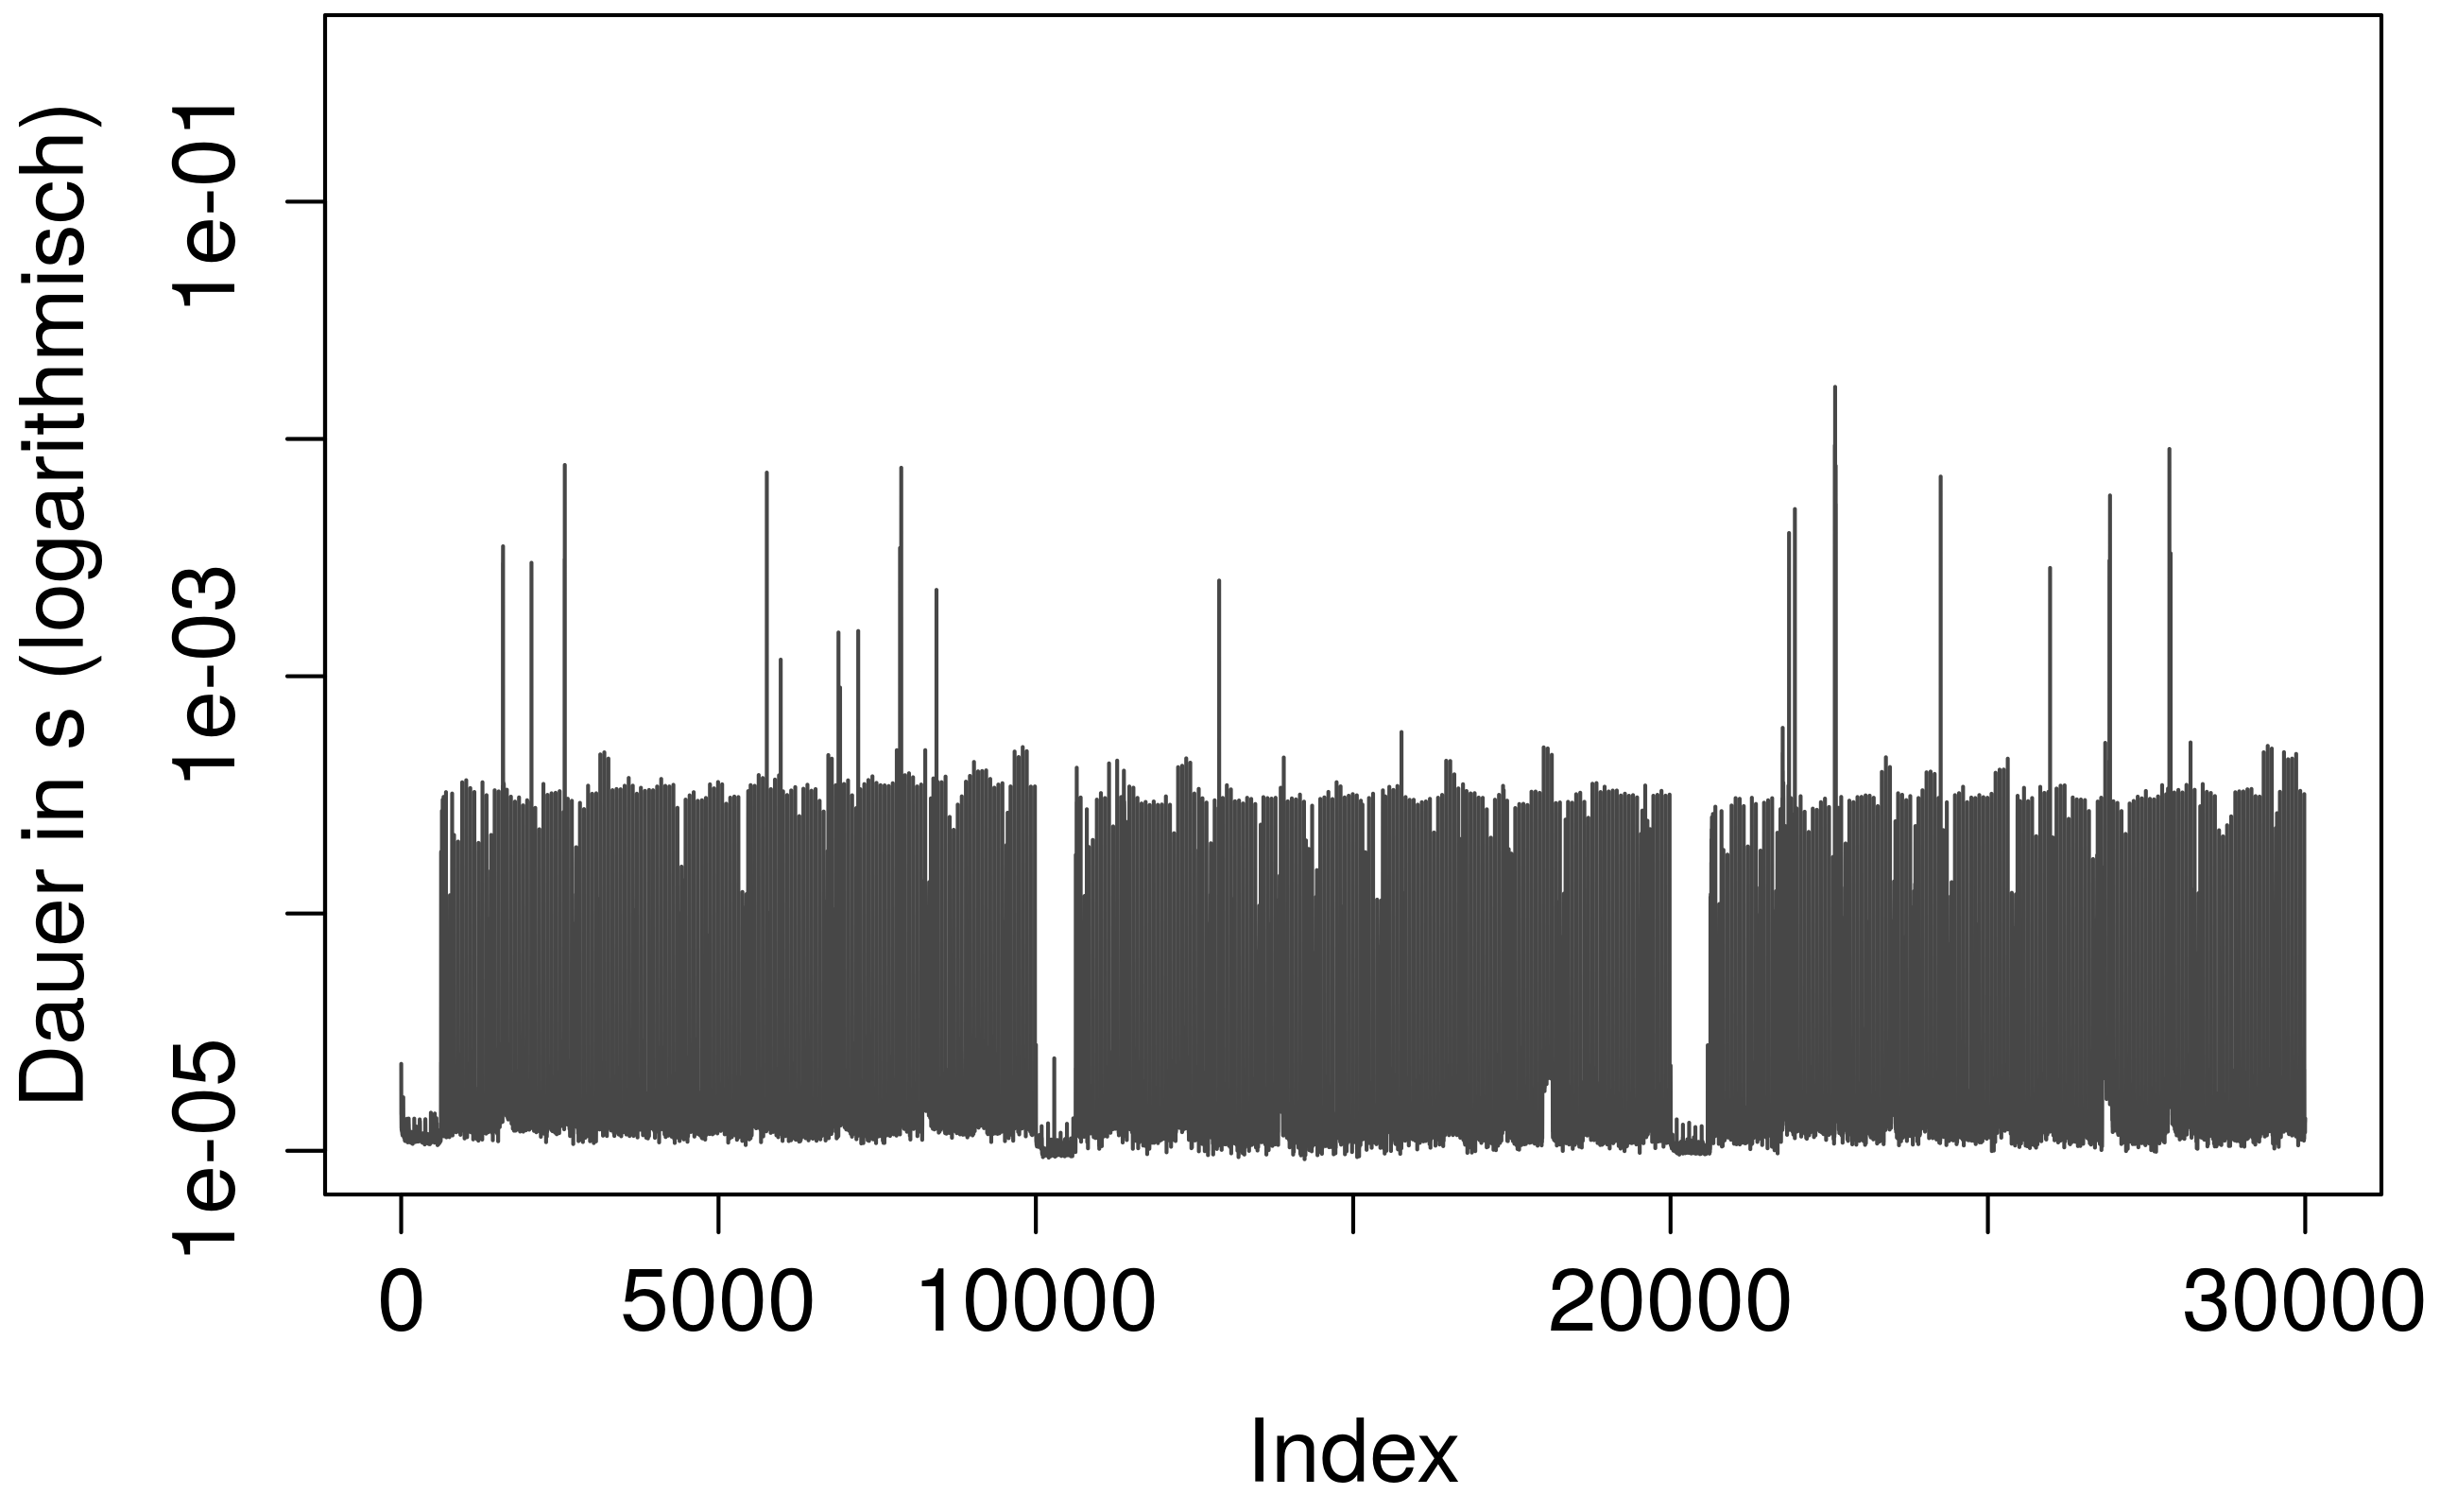
\includegraphics[width=.43\textwidth]{Bilder/Plots/exploration/plot_Size16384_read_seq.png}
	}
	\hfill
	\subfloat[Sequentiell schreibend]{
		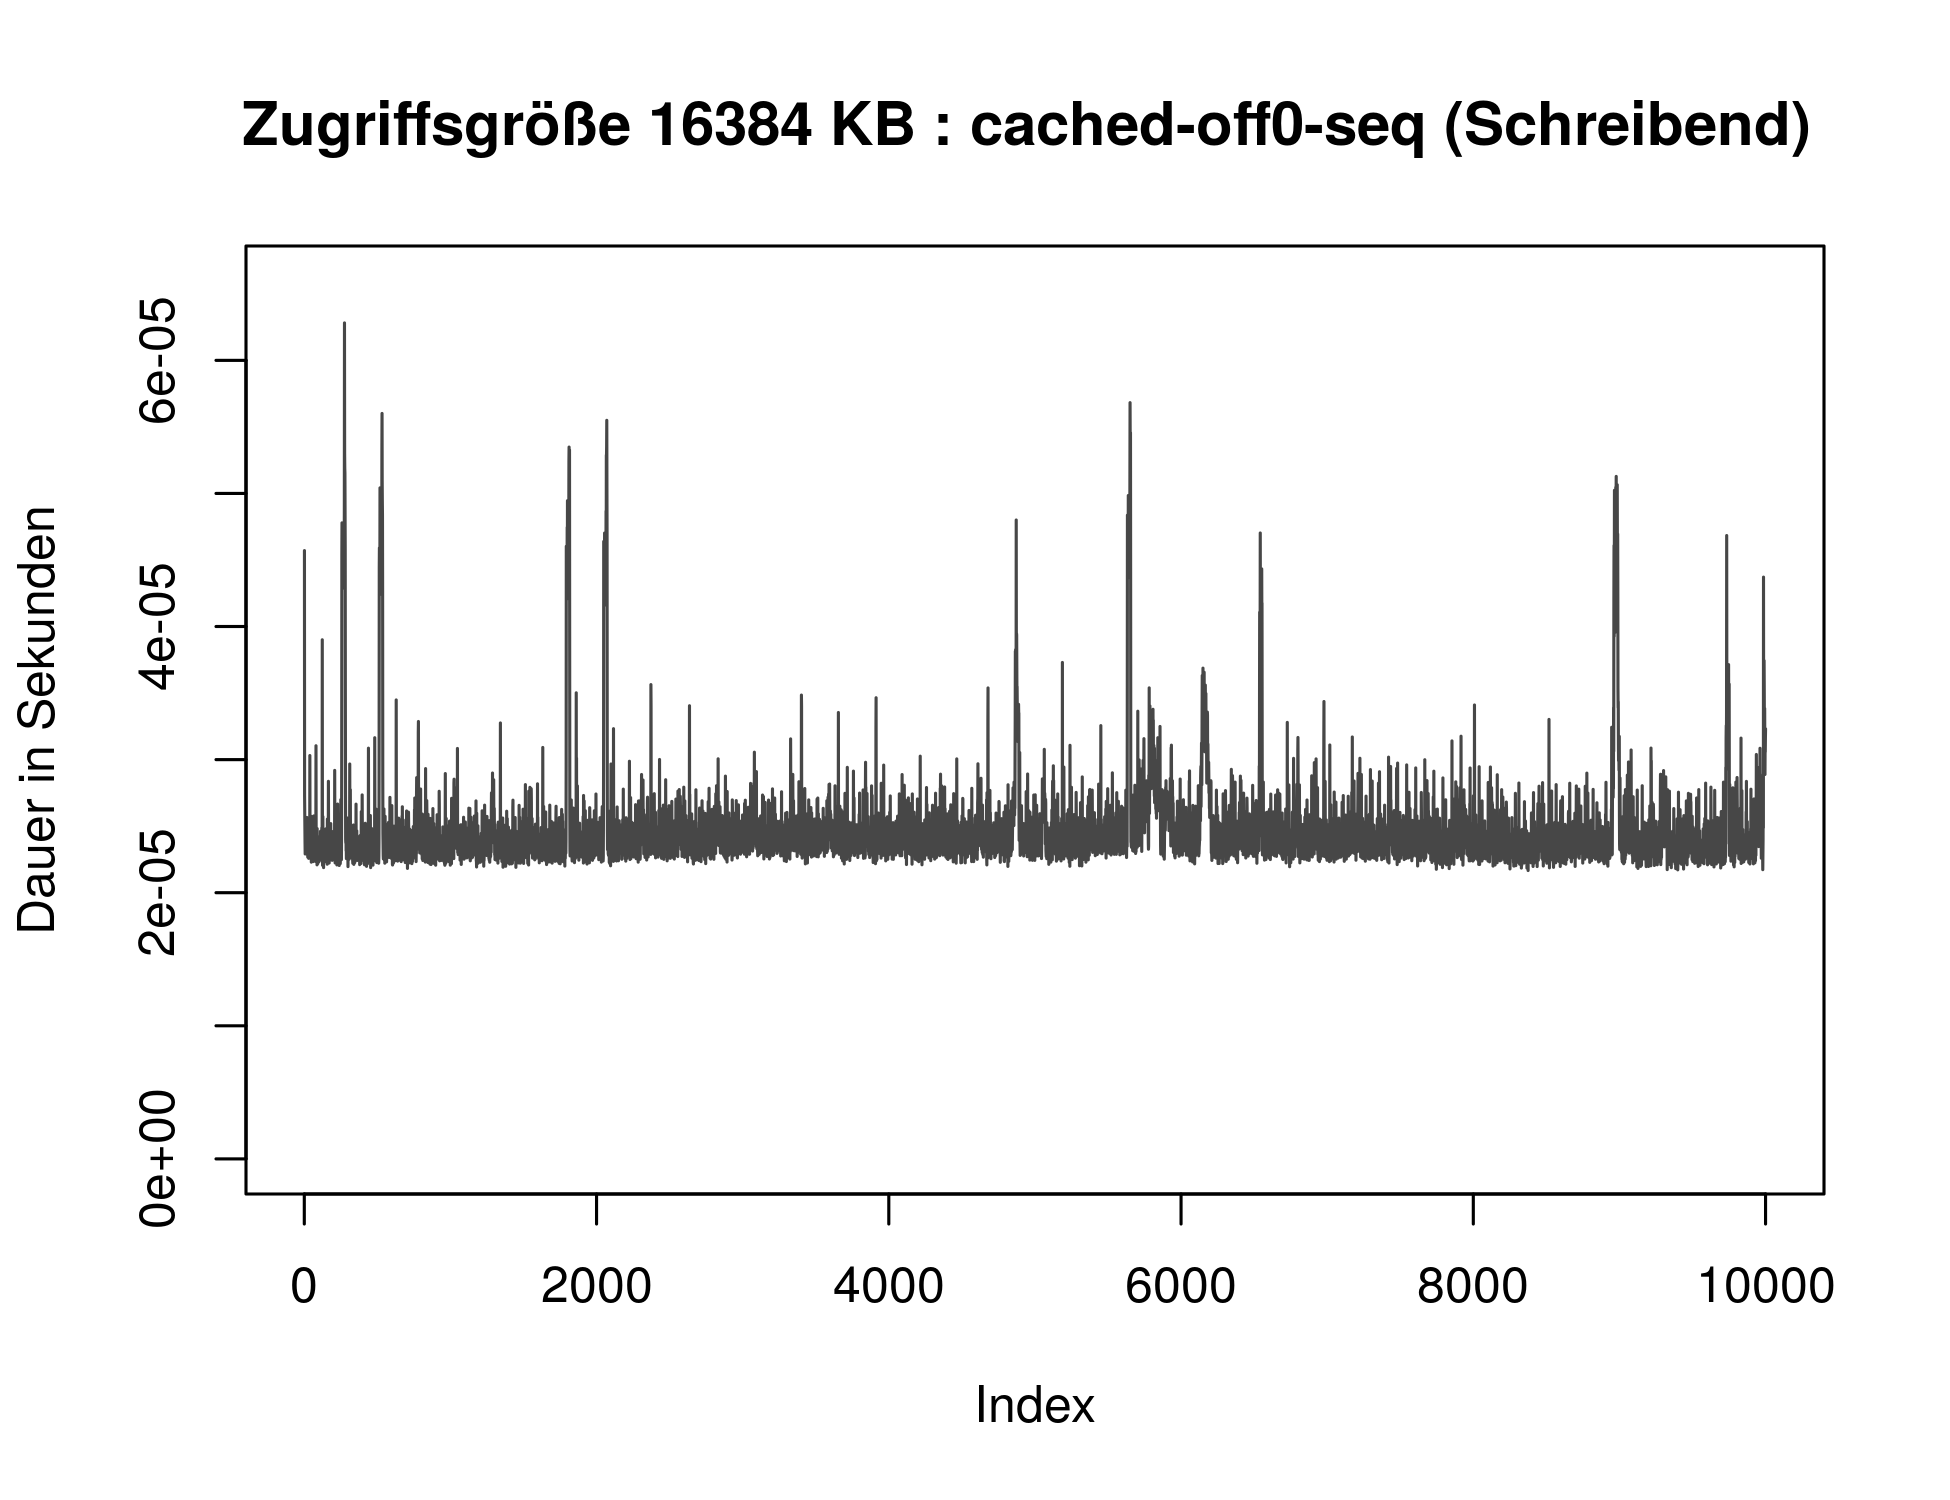
\includegraphics[width=.43\textwidth]{Bilder/Plots/exploration/plot_Size16384_write_seq.png}
	}\\
	\subfloat[Randomisiert lesend]{
		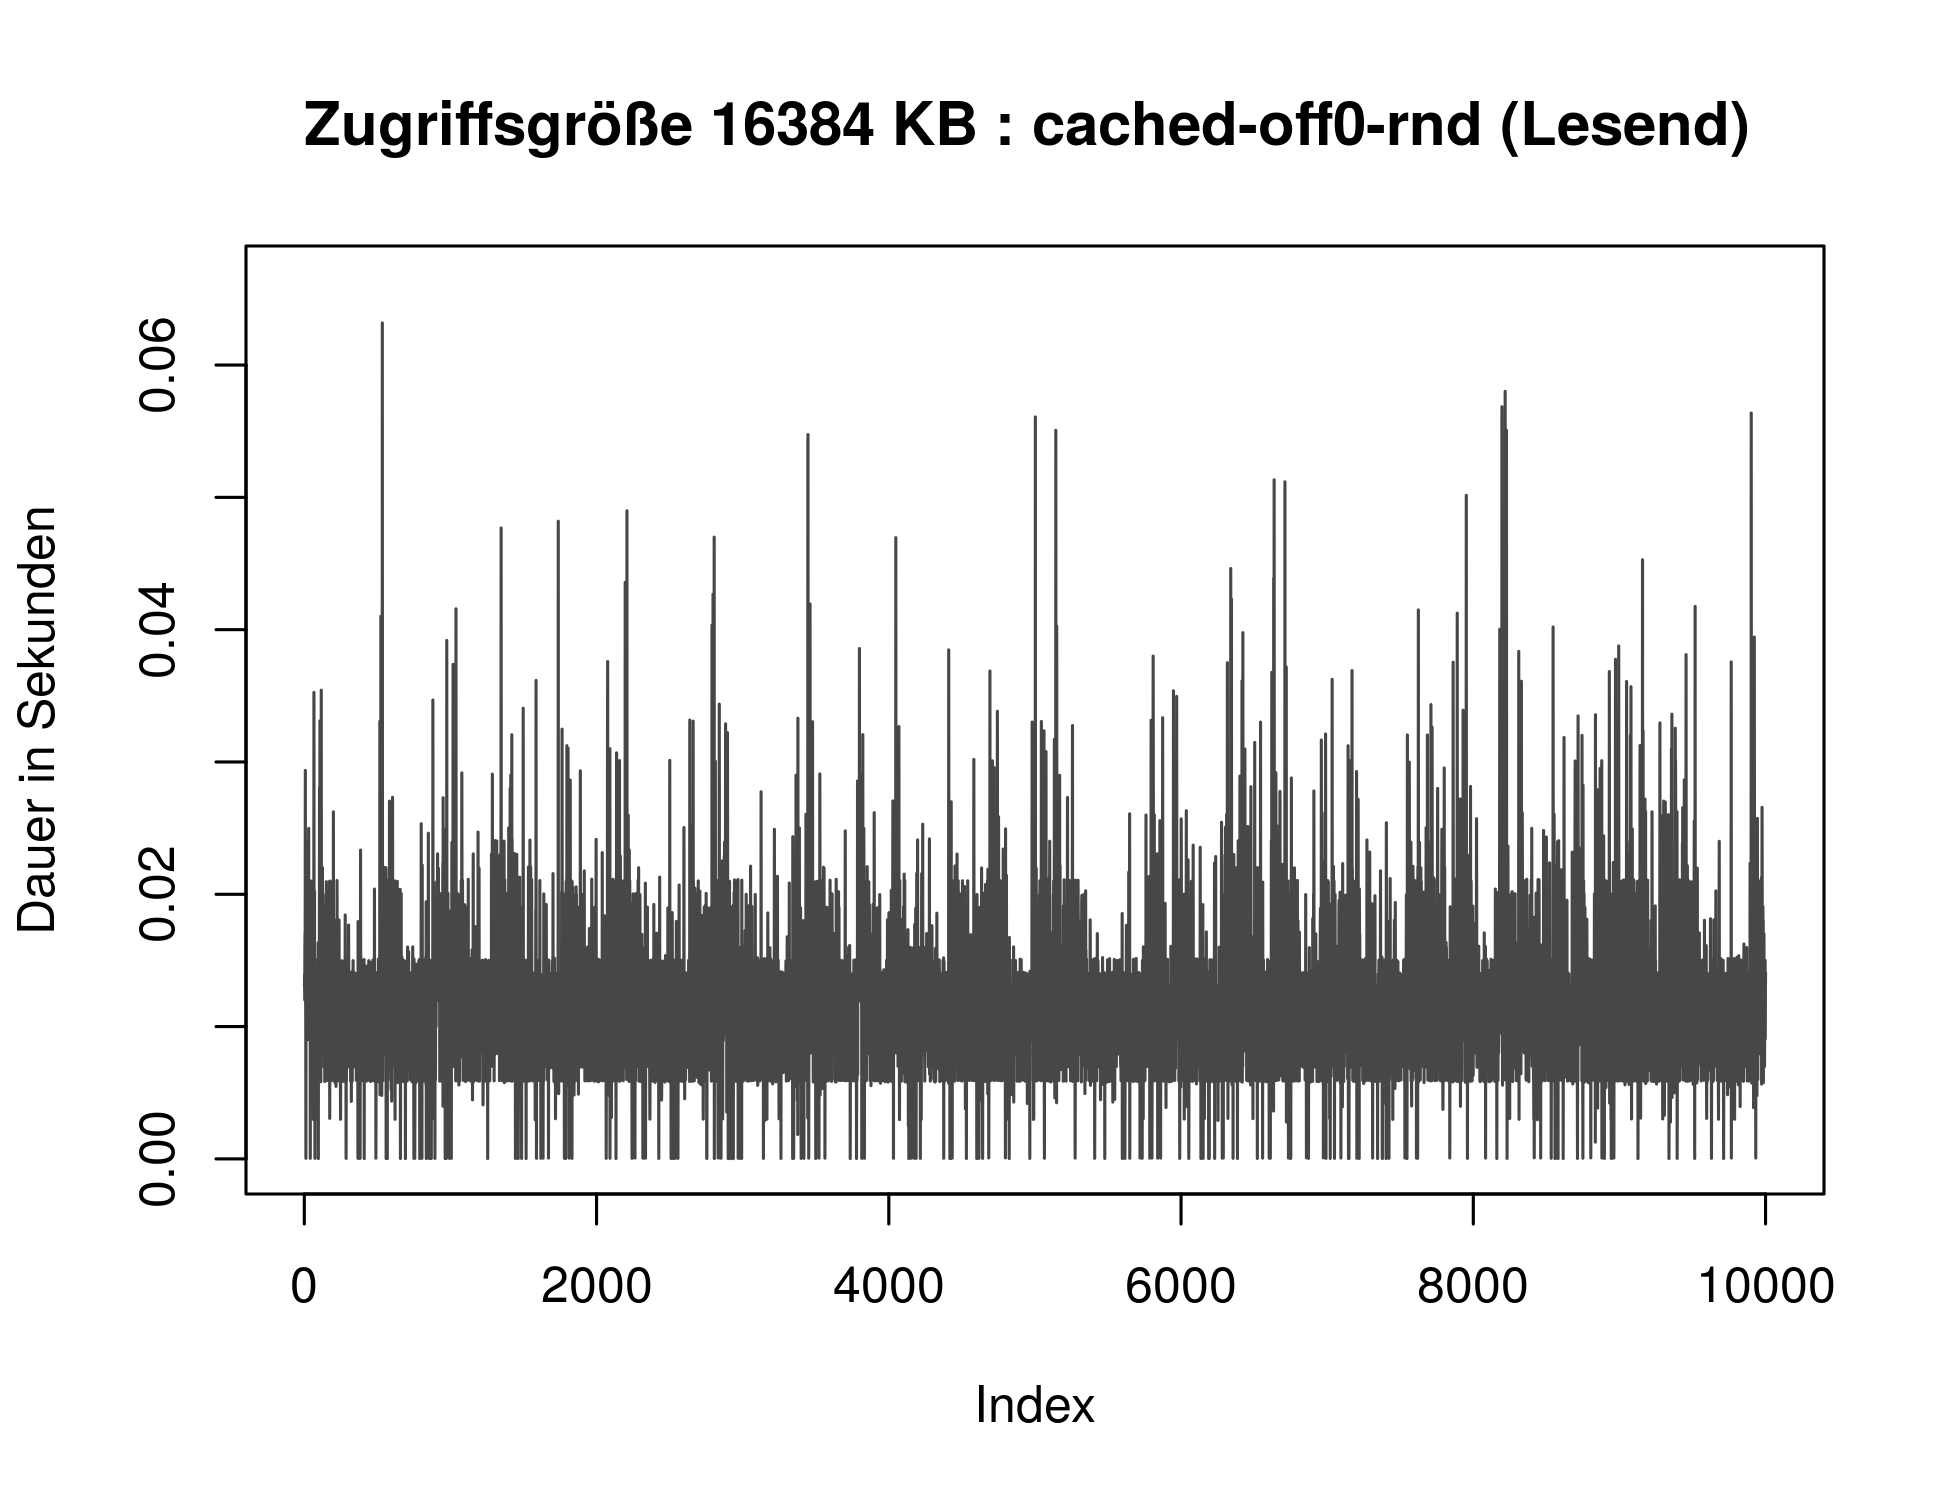
\includegraphics[width=.43\textwidth]{Bilder/Plots/exploration/plot_Size16384_read_rnd.png}
	}
	\hfill
	\subfloat[Randomisiert schreibend]{
		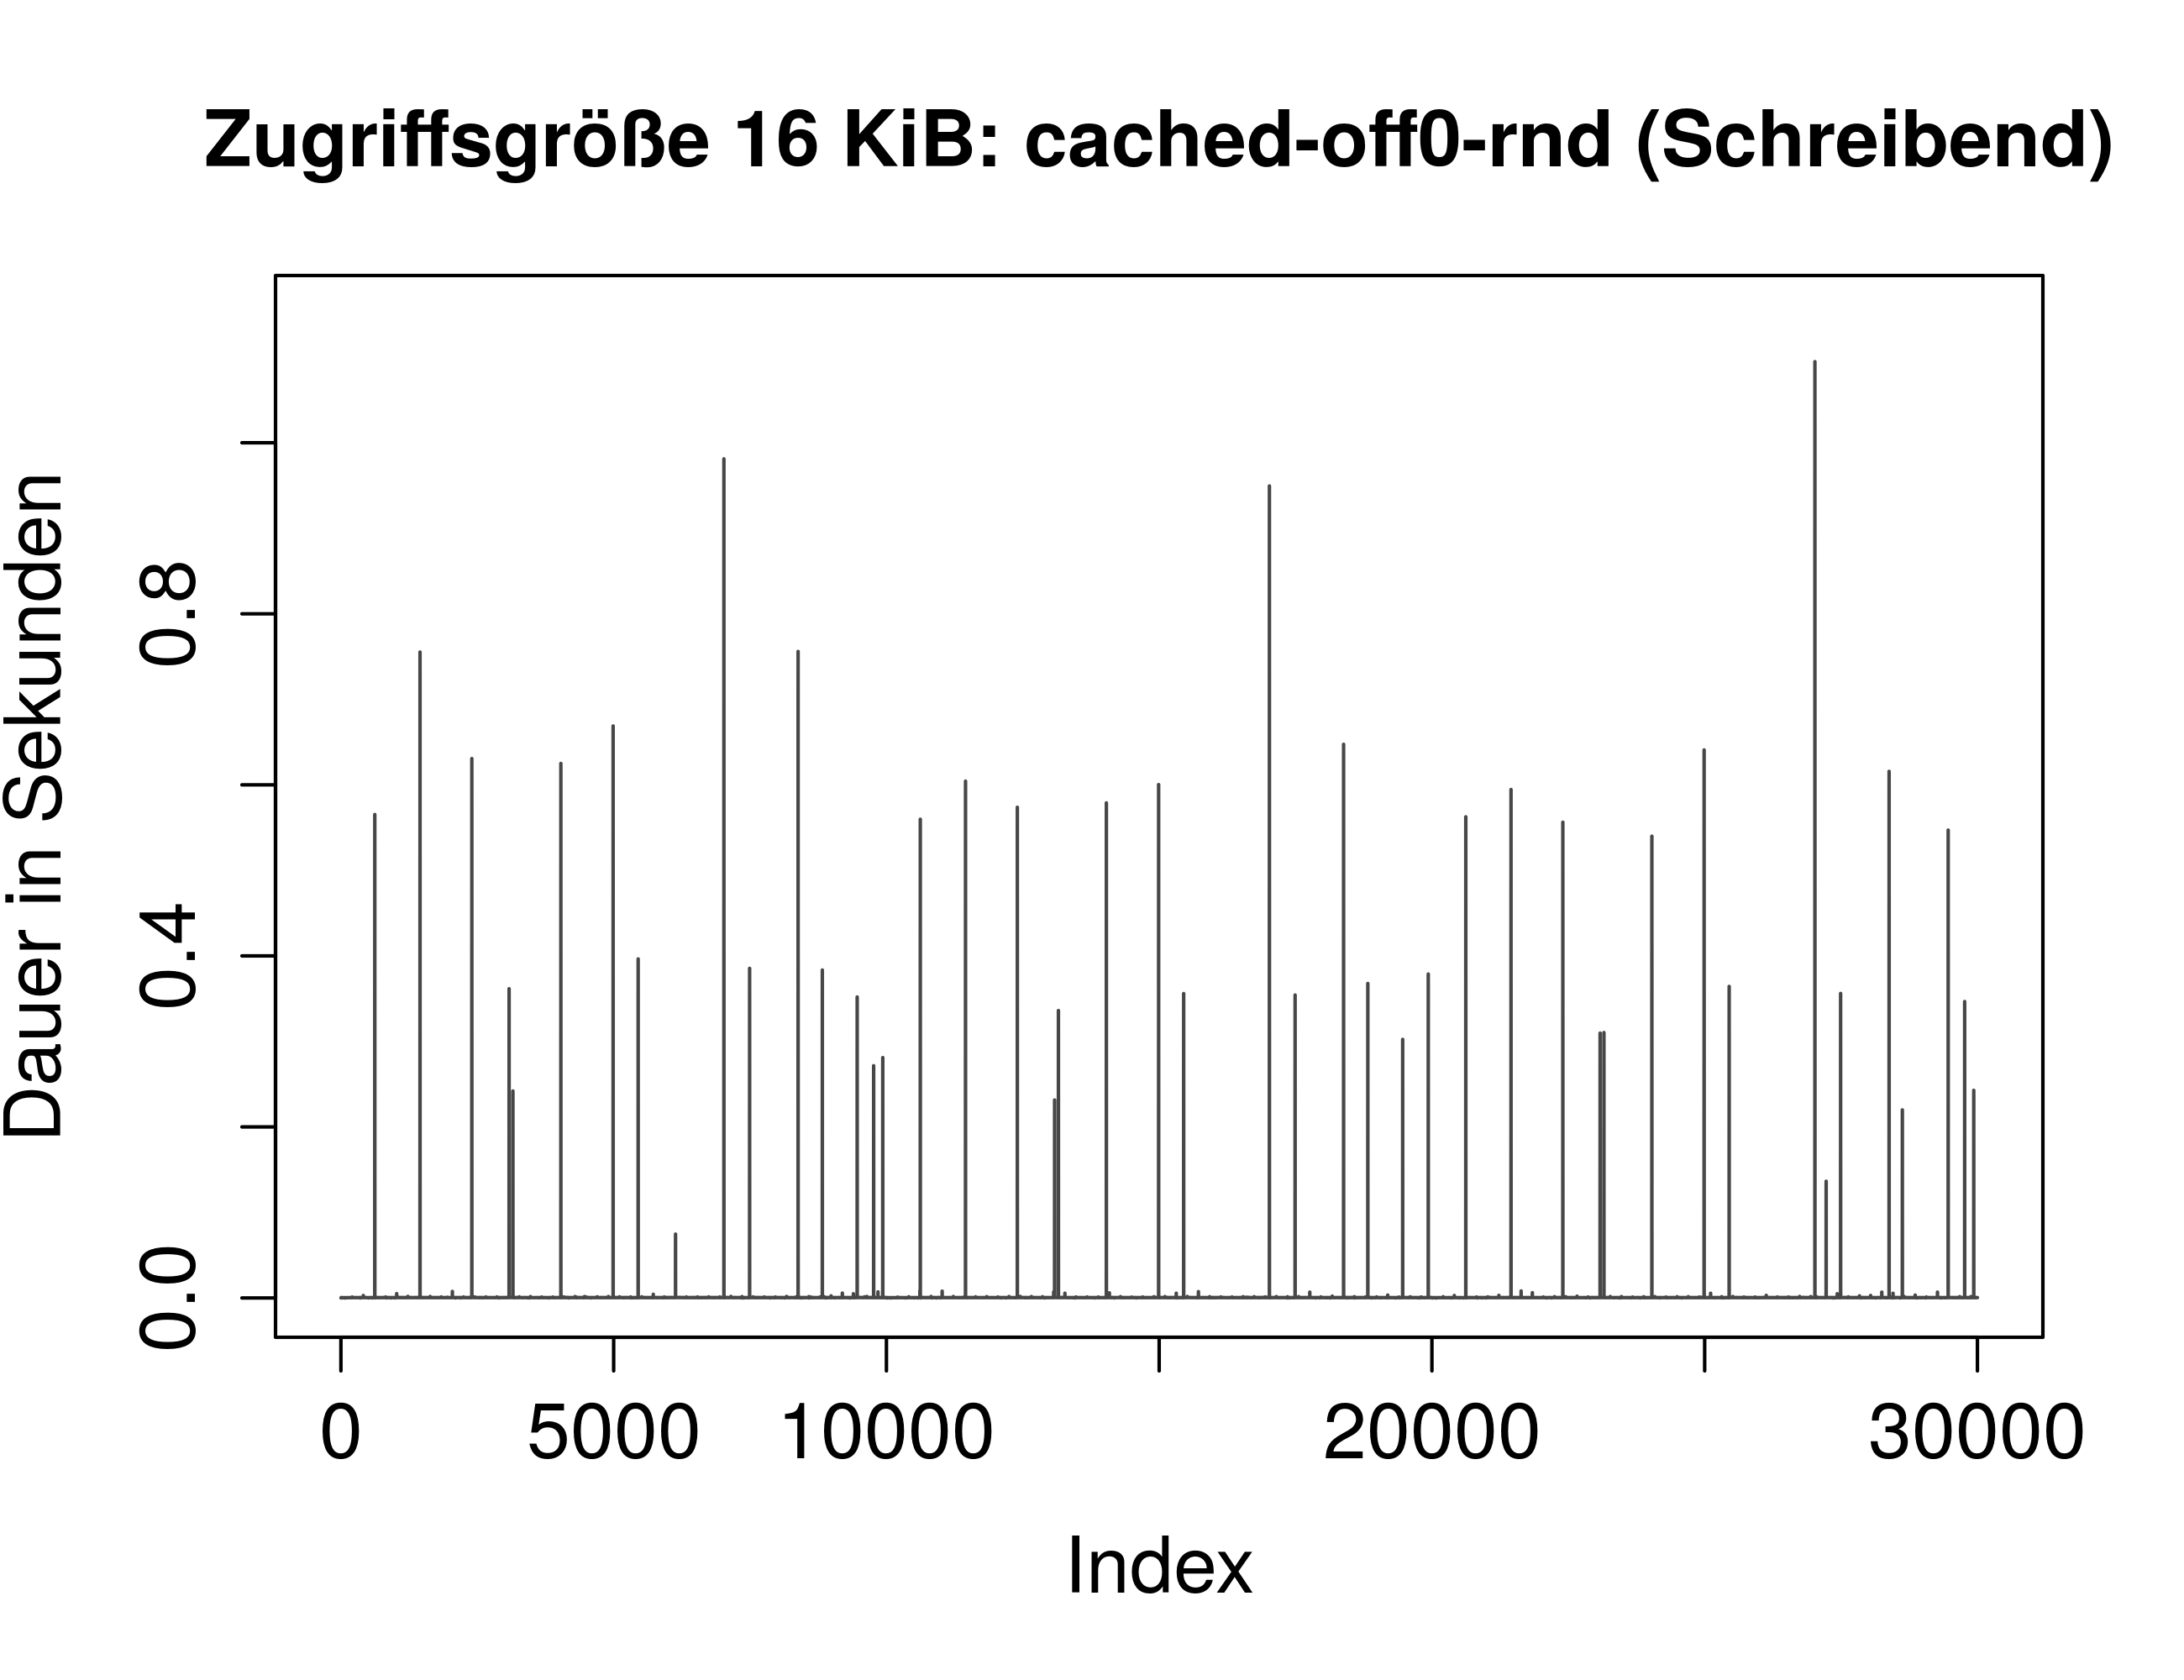
\includegraphics[width=.43\textwidth]{Bilder/Plots/exploration/plot_Size16384_write_rnd.png}
	}		
	\vspace*{-0.3cm}
	\caption{Detailbetrachtung aller Messungen mit Zugriffsgröße 16KiB}
	\label{fig:groesse16384}
\end{figure}
\begin{figure}
	\subfloat[Sequentiell lesend]{
		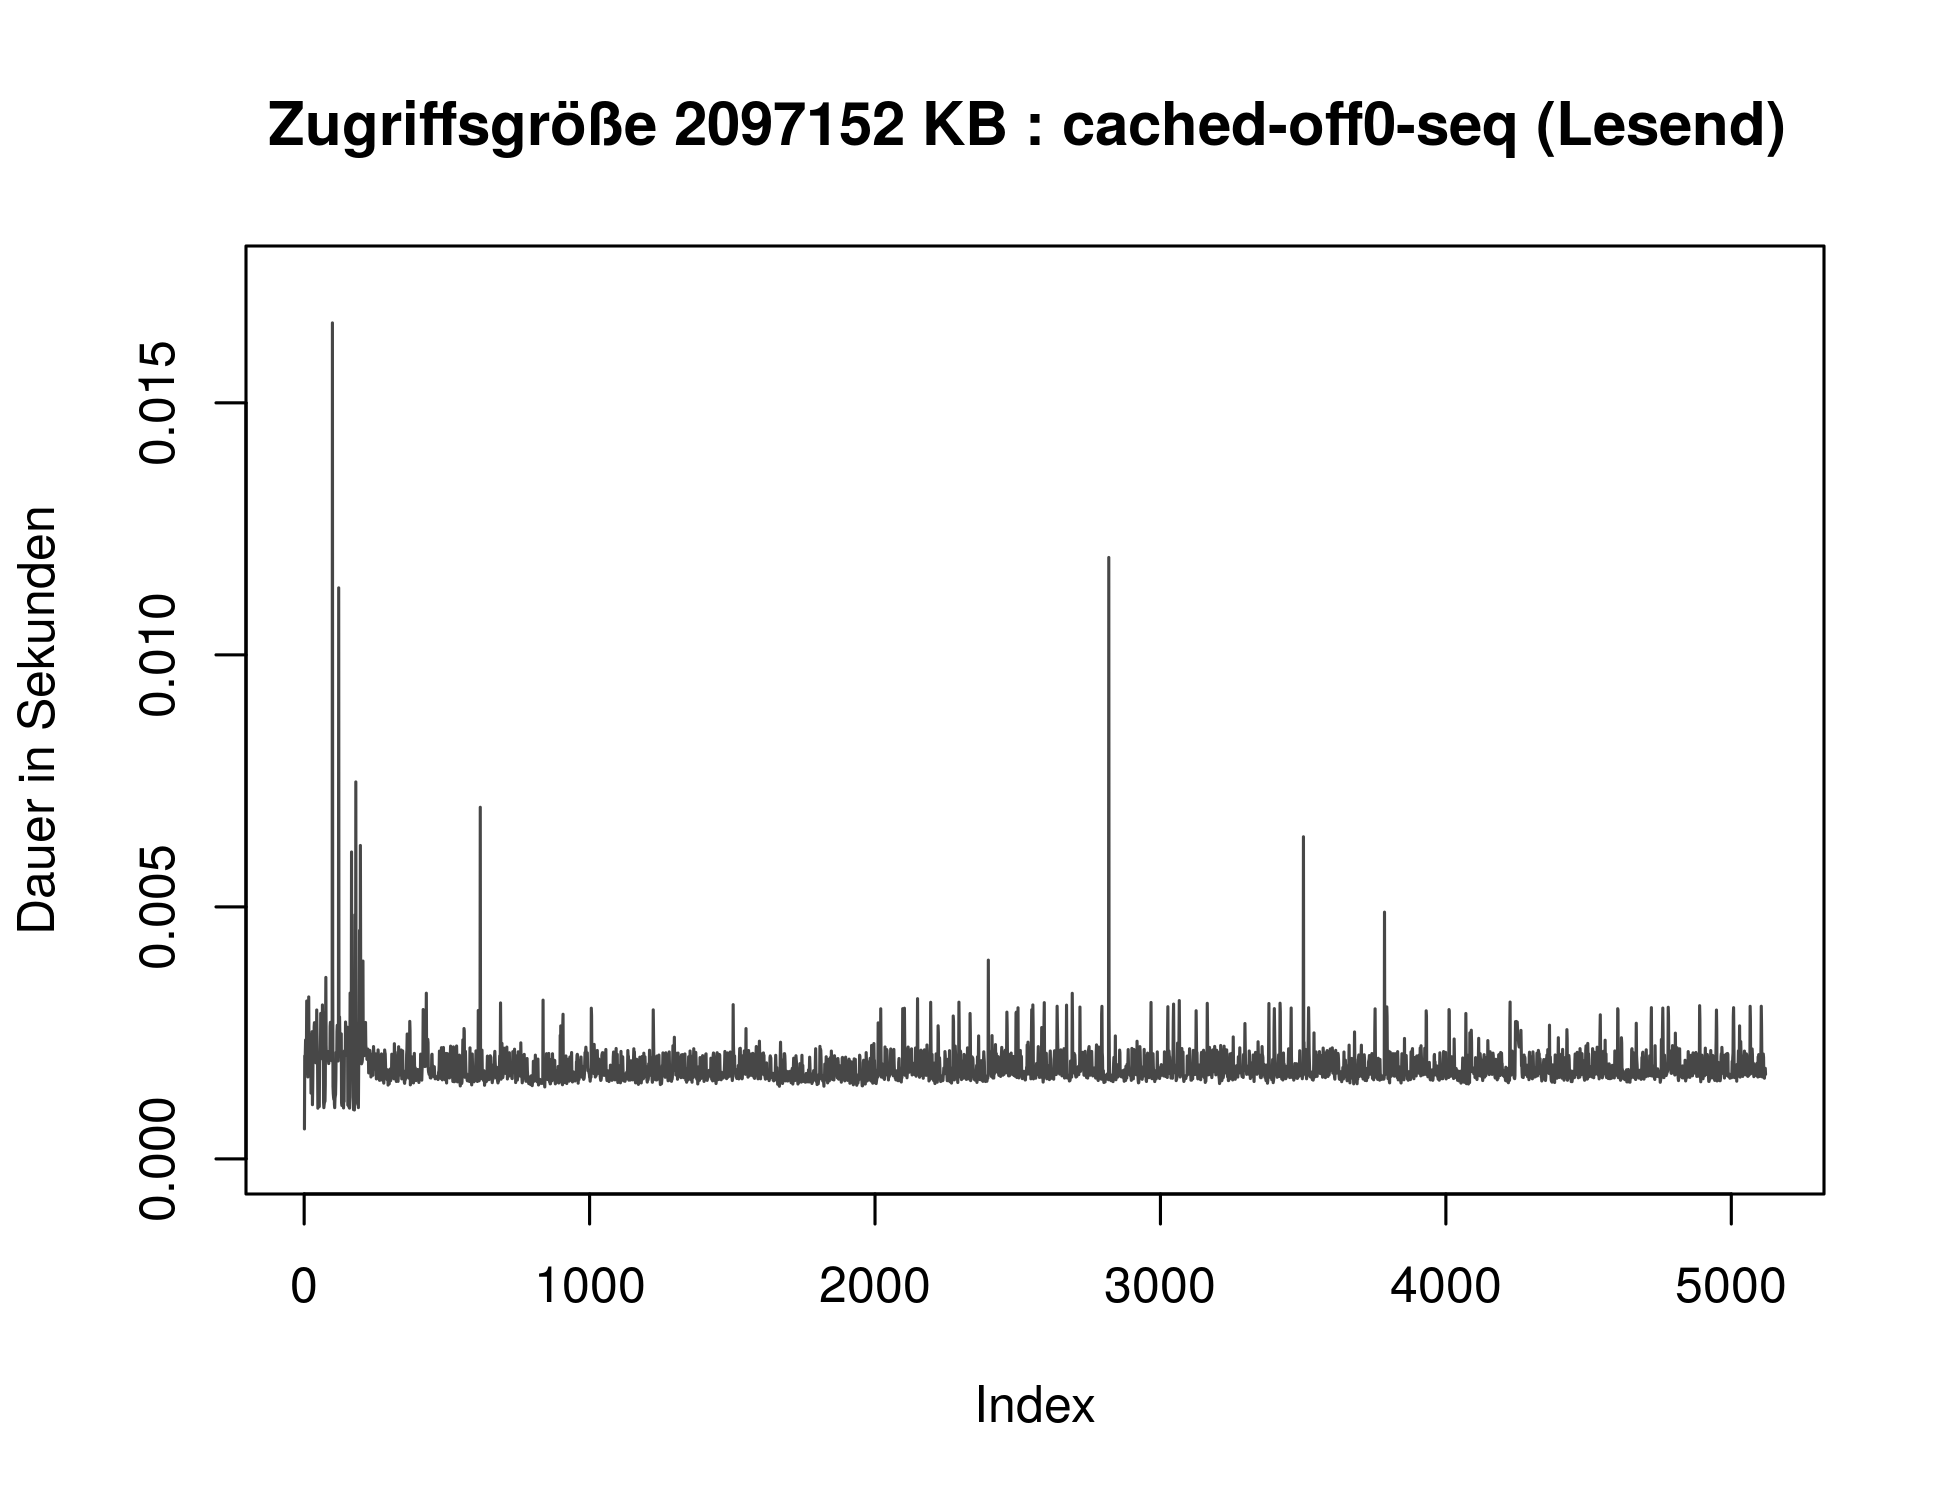
\includegraphics[width=.43\textwidth]{Bilder/Plots/exploration/plot_Size2097152_read_seq.png}
	}
	\hfill
	\subfloat[Sequentiell schreibend]{
		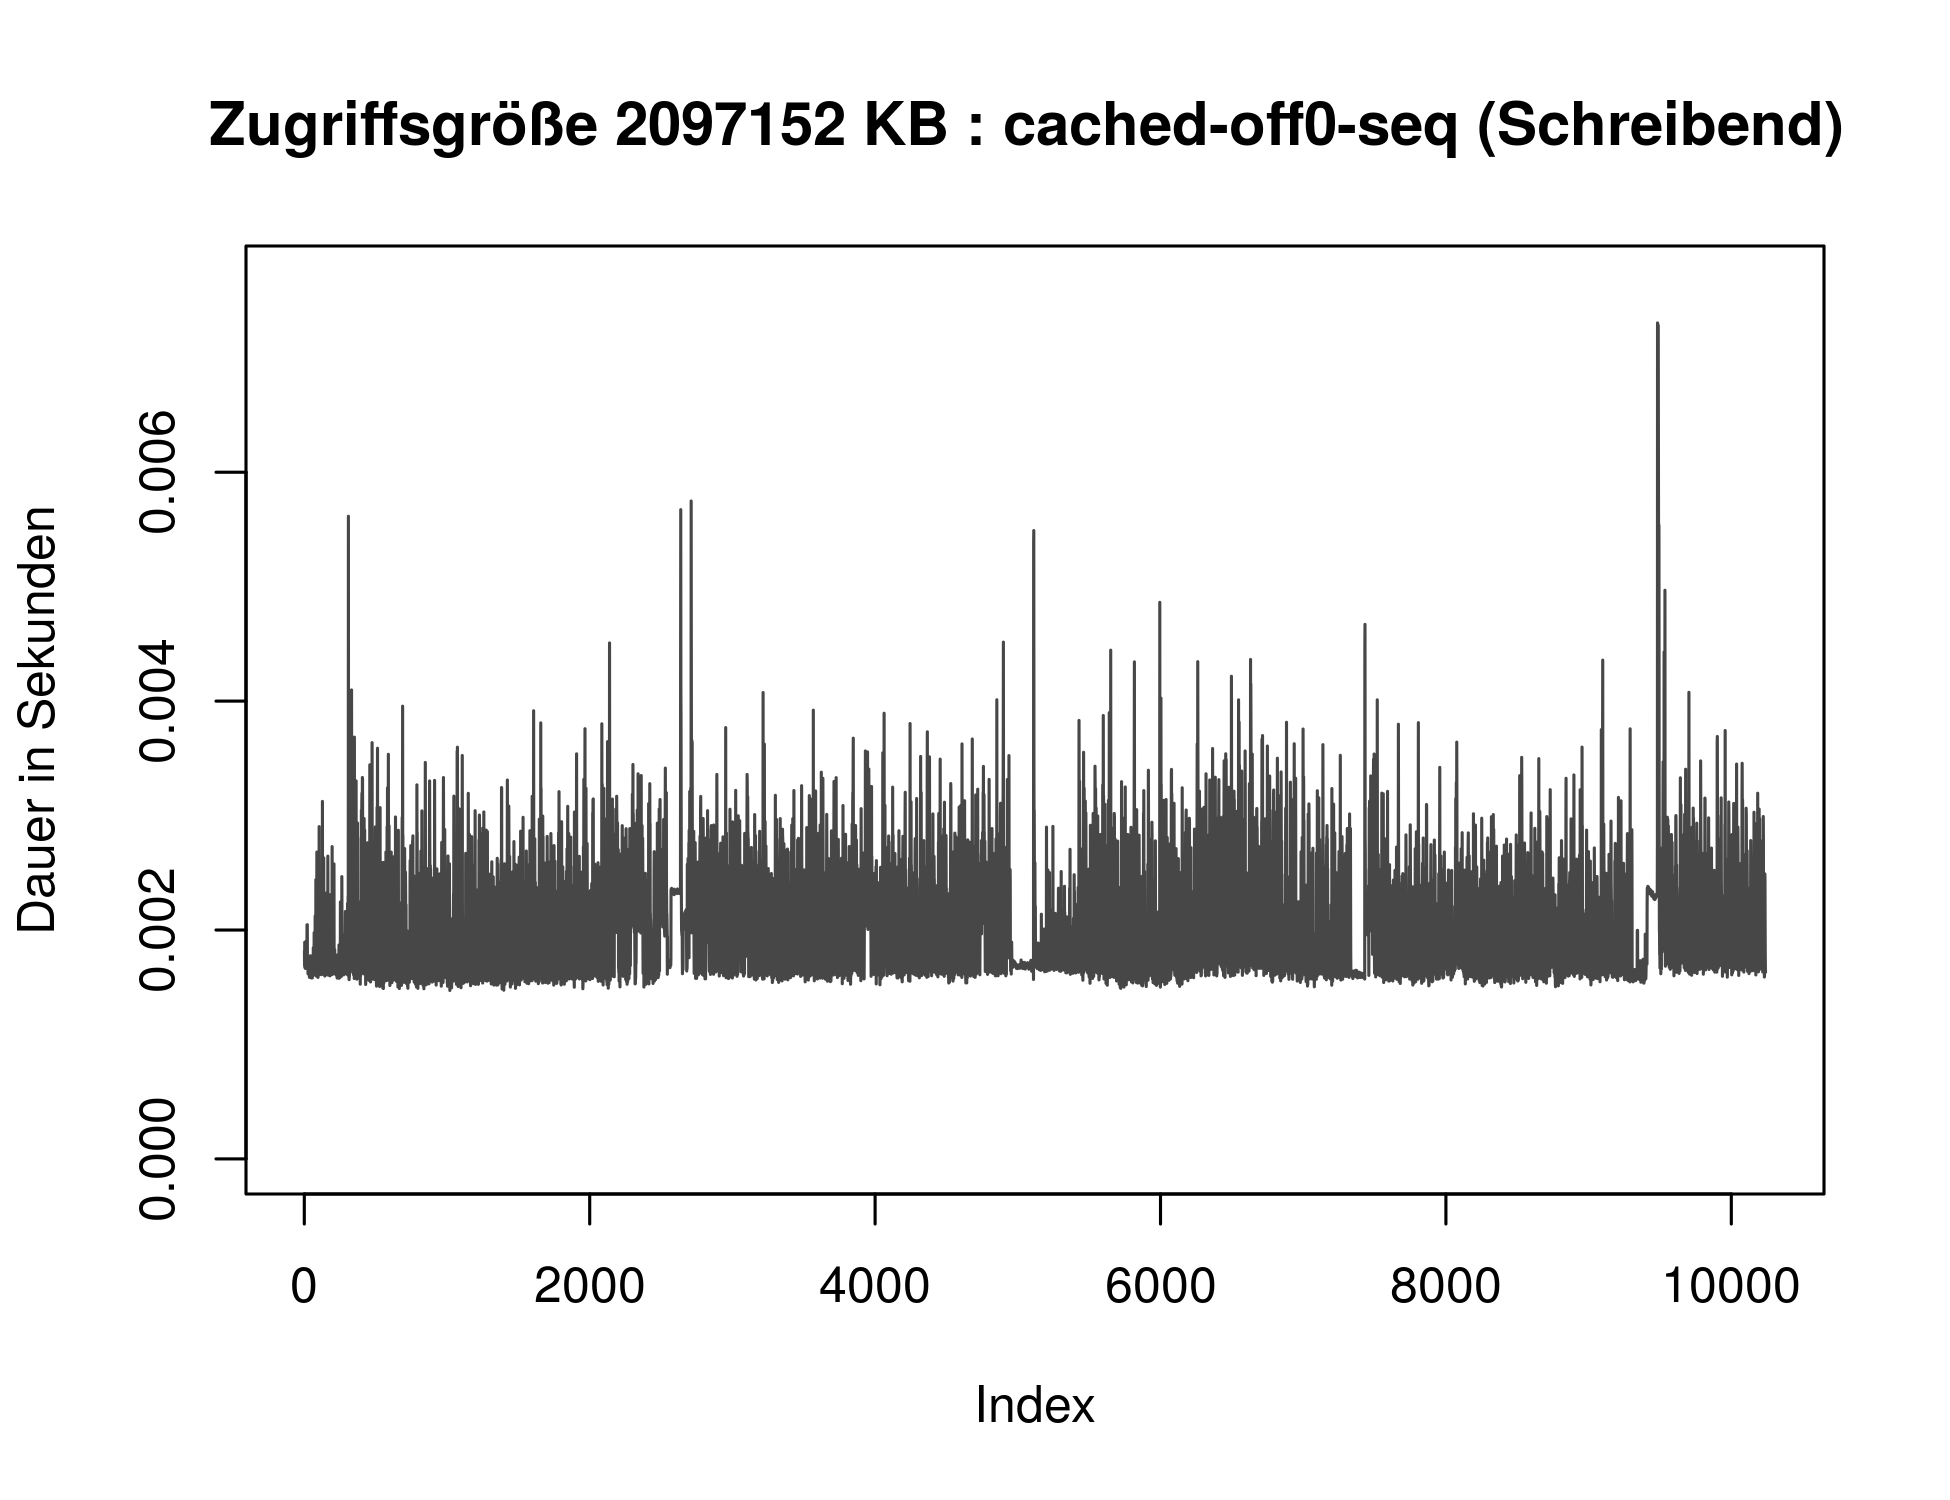
\includegraphics[width=.43\textwidth]{Bilder/Plots/exploration/plot_Size2097152_write_seq.png}
	}\\
	\subfloat[Randomisiert lesend]{
		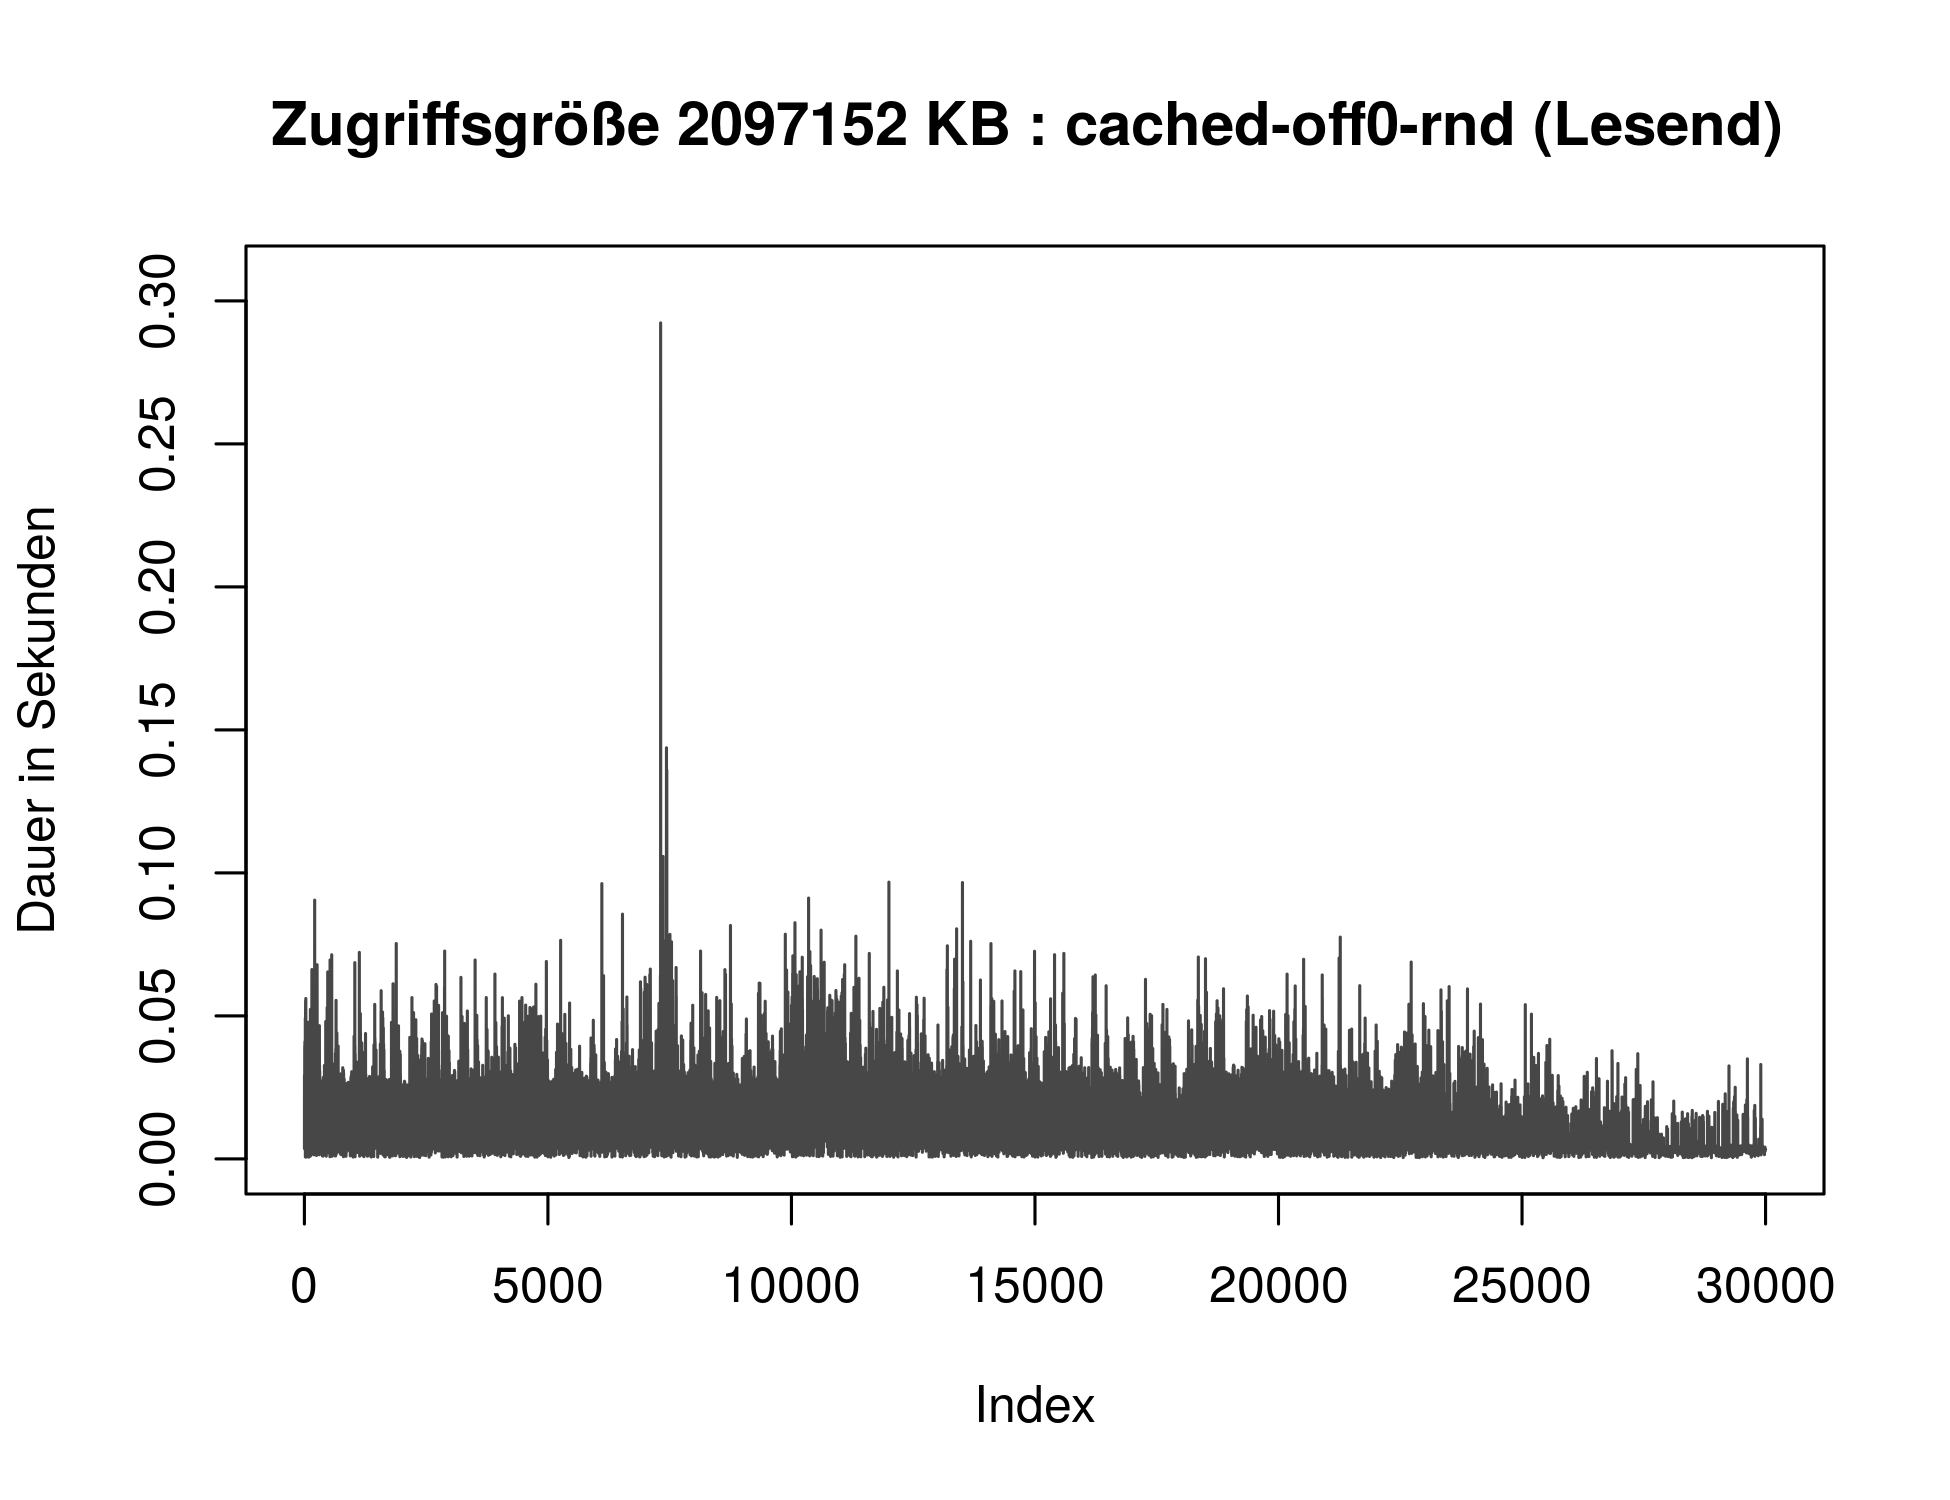
\includegraphics[width=.43\textwidth]{Bilder/Plots/exploration/plot_Size2097152_read_rnd.png}
	}
	\hfill
	\subfloat[Randomisiert schreibend]{
		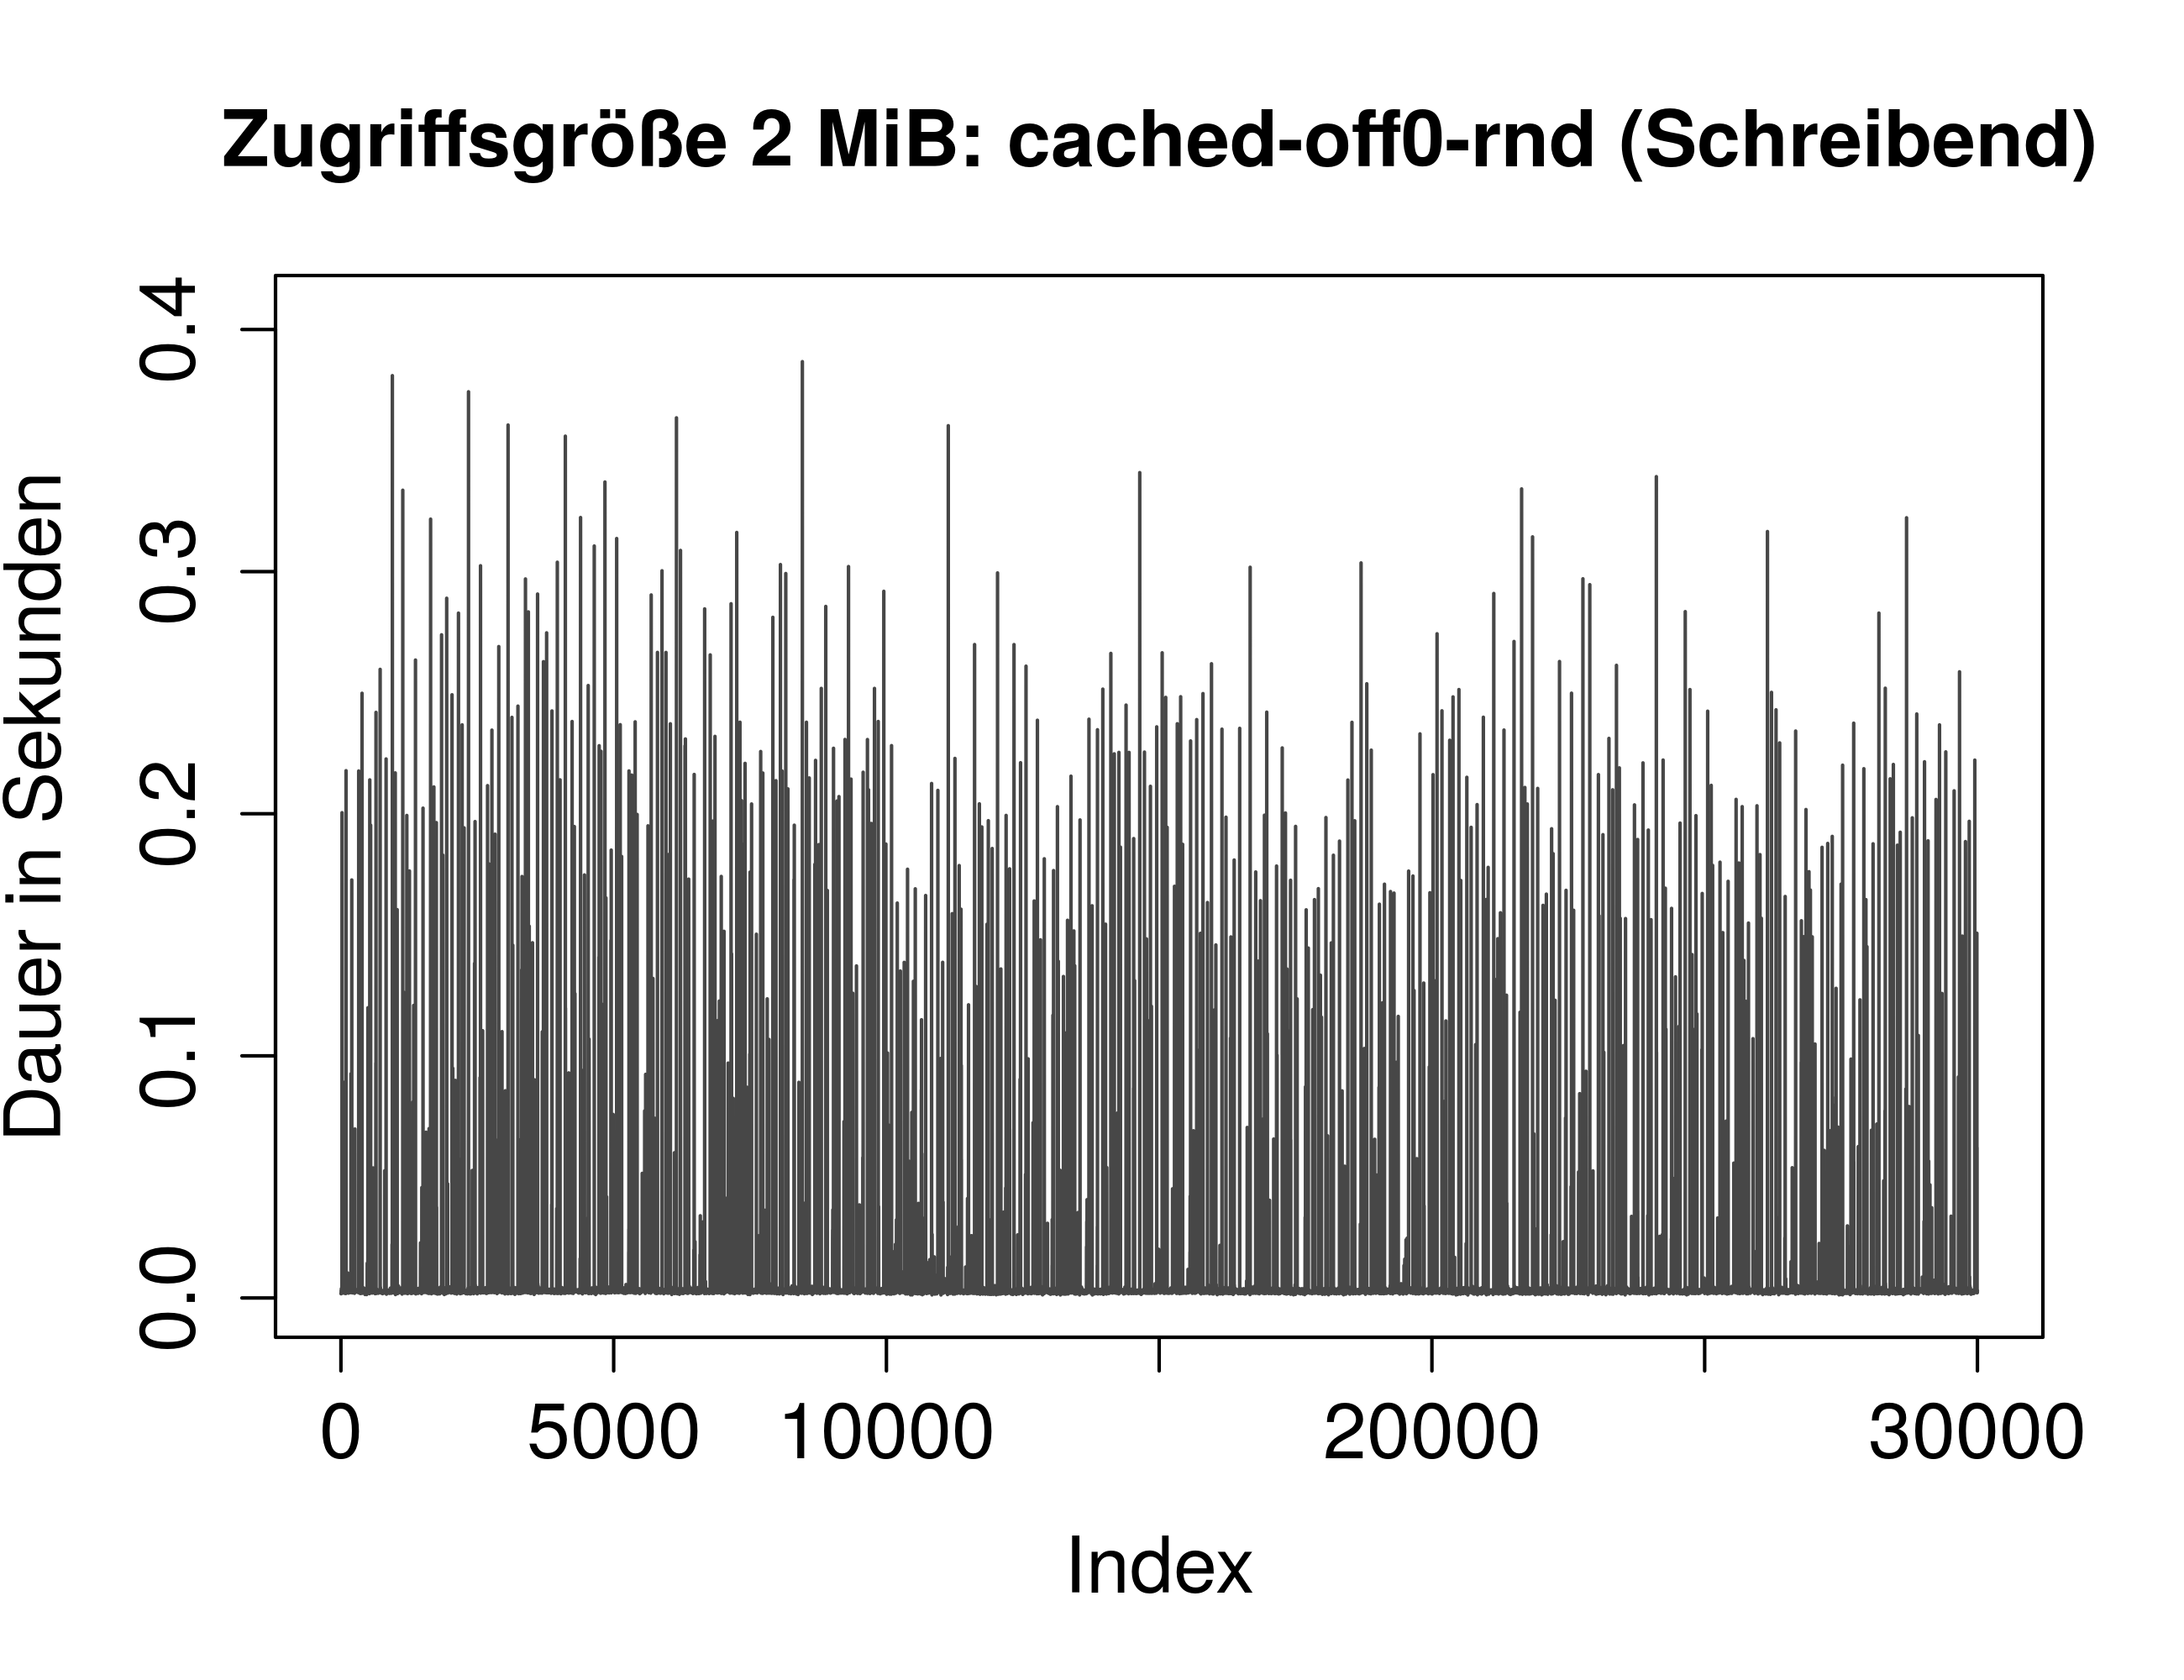
\includegraphics[width=.43\textwidth]{Bilder/Plots/exploration/plot_Size2097152_write_rnd.png}
	}		
	\vspace*{-0.3cm}
	\caption{Detailbetrachtung aller Messungen mit Zugriffsgröße 2MiB}
	\label{fig:groesse2097152}
\end{figure}

Um die Messdaten noch detaillierter darzustellen, müssen kleine Ausschnitte herausgegriffen werden. Zunächst betrachte ich die ersten $250$ Messungen. \ref{fig:first250}
Auf dem ersten Blick scheint bei seq-W eine gewisse Periodizität ersichtlich. Etwa alle 45 Messungen gibt es einen größeren Sprung, alternierend sind die Laufzeiten jeweils etwas langsamer und schneller.
Nach genau $123$ Punkten scheint sich das Muster zu wiederholen, dort befindet sich der zweitgrößte Messwert. Wenn man nun als erstes simples Modell eine Fortführung der augenscheinlichen Periodizität der ersten $123$ Messpunkten betrachtet, so erkannt man doch, dass der Verlauf recht unregelmäßig ist. \ref{fig:periodicity}
Bei den anderen Graphen kann keine so simple Periodizität beobachtet werden.

\begin{figure}
	\subfloat[Sequentiell lesend]{
		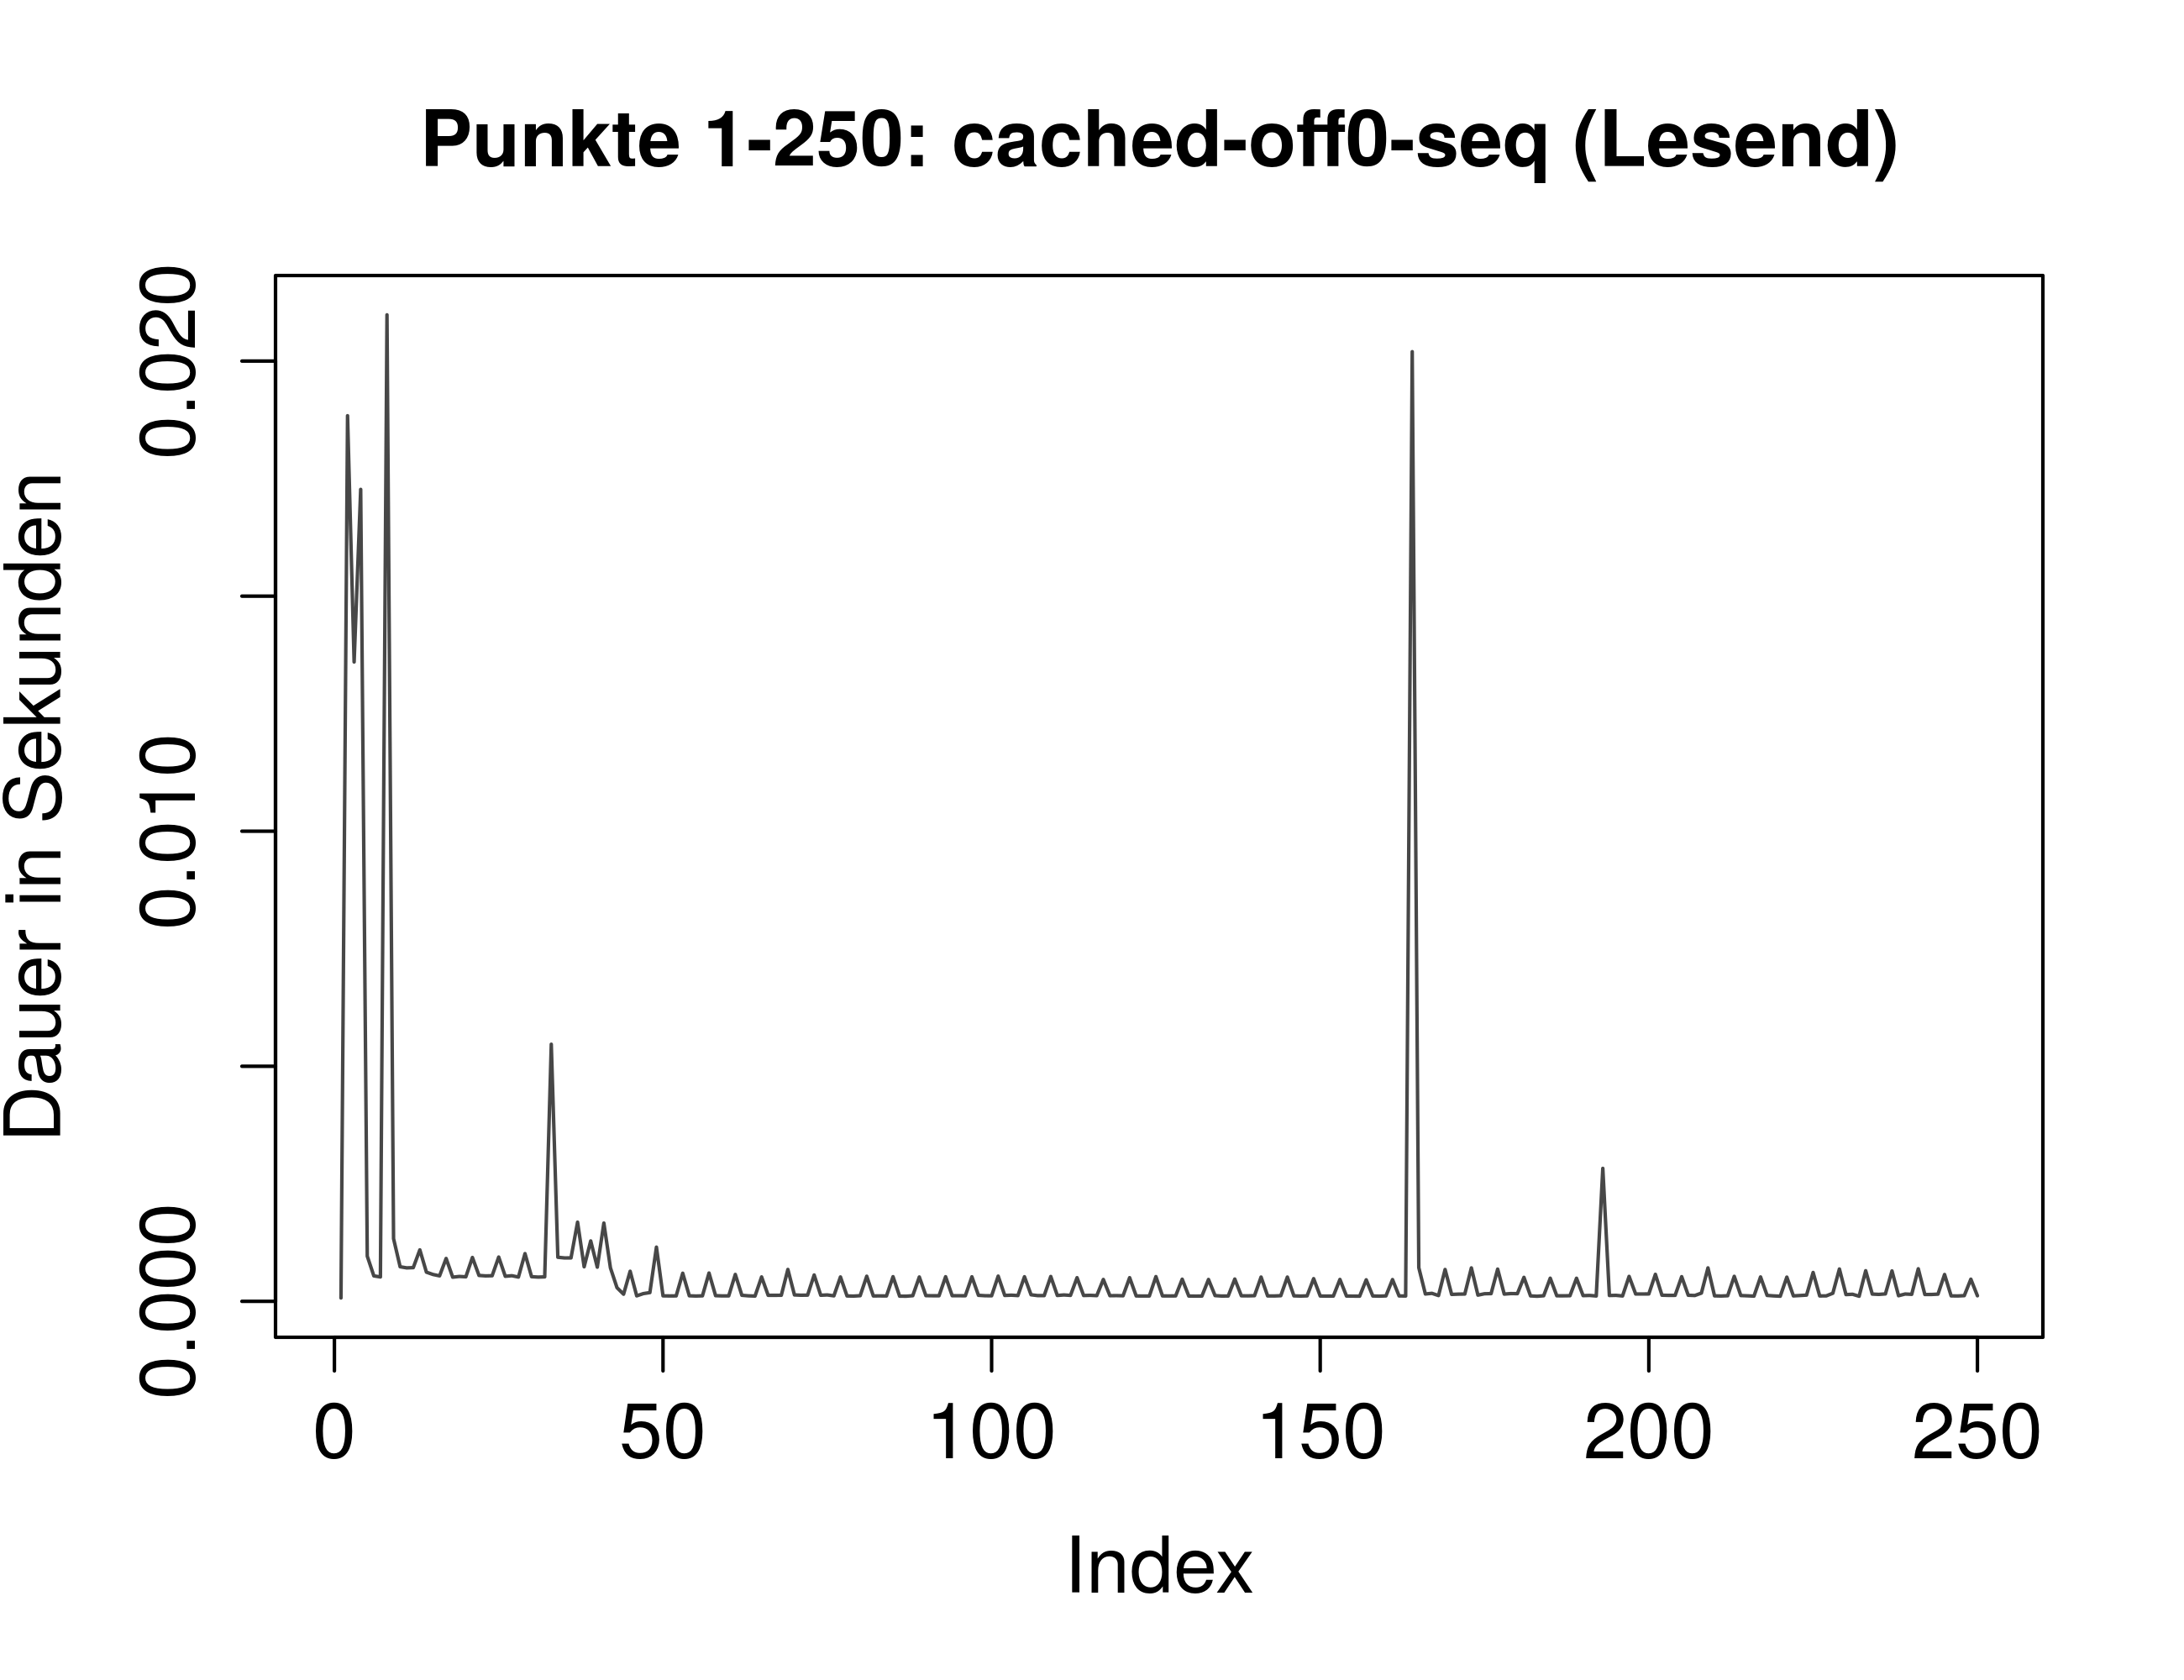
\includegraphics[width=.43\textwidth]{Bilder/Plots/exploration/plot_First250_read_seq.png}
	}
	\hfill
	\subfloat[Sequentiell schreibend]{
		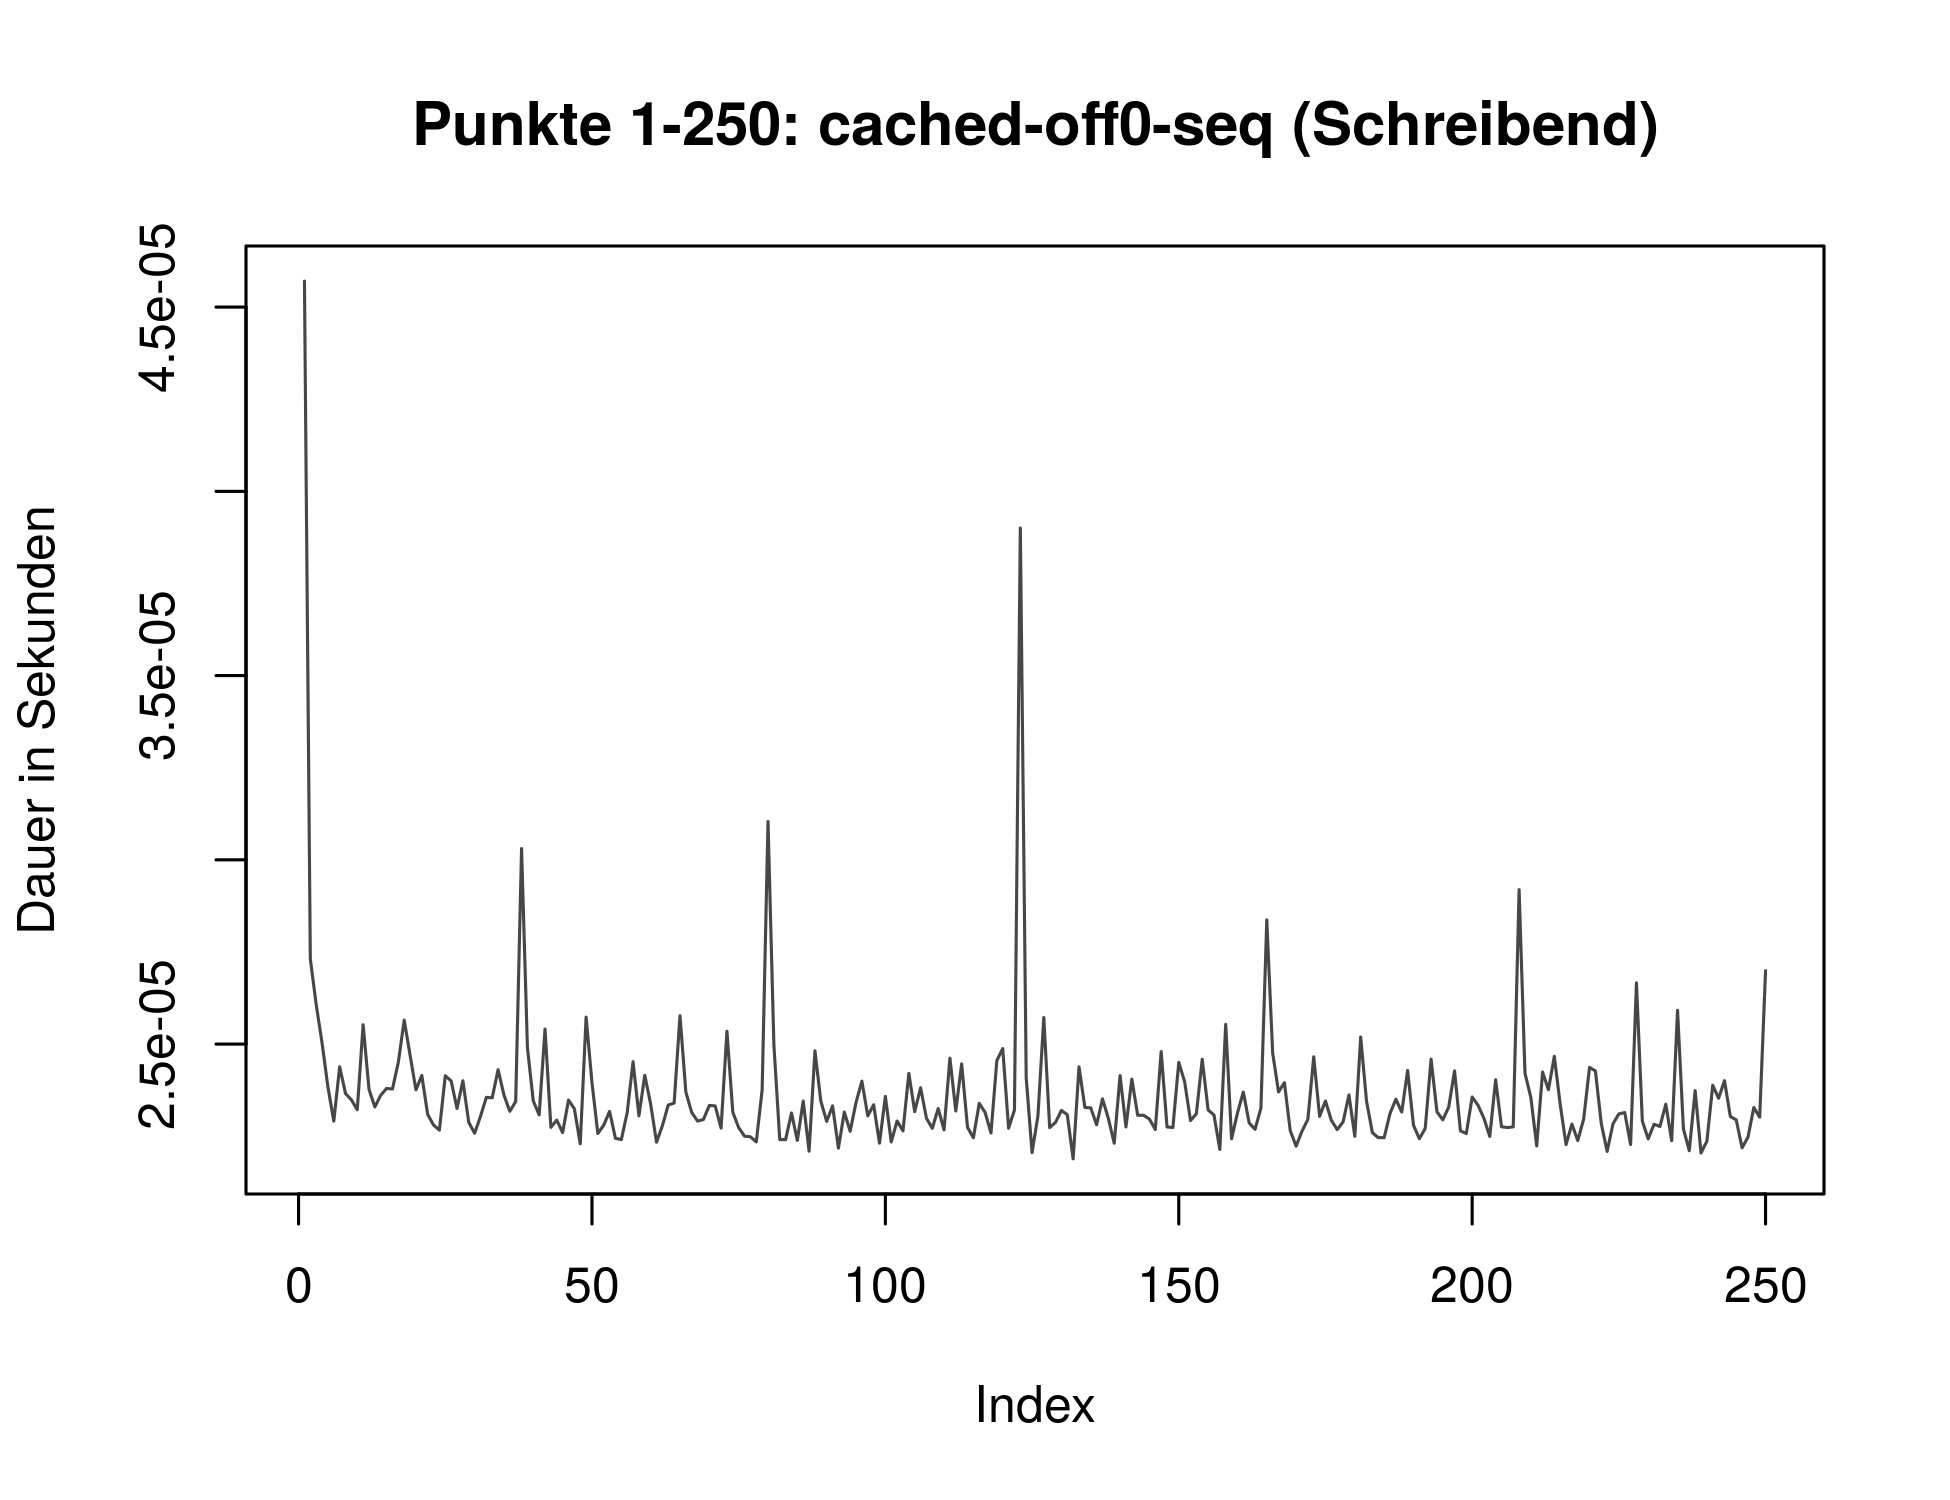
\includegraphics[width=.43\textwidth]{Bilder/Plots/exploration/plot_First250_write_seq.png}
	}\\
	\subfloat[Randomisiert lesend]{
		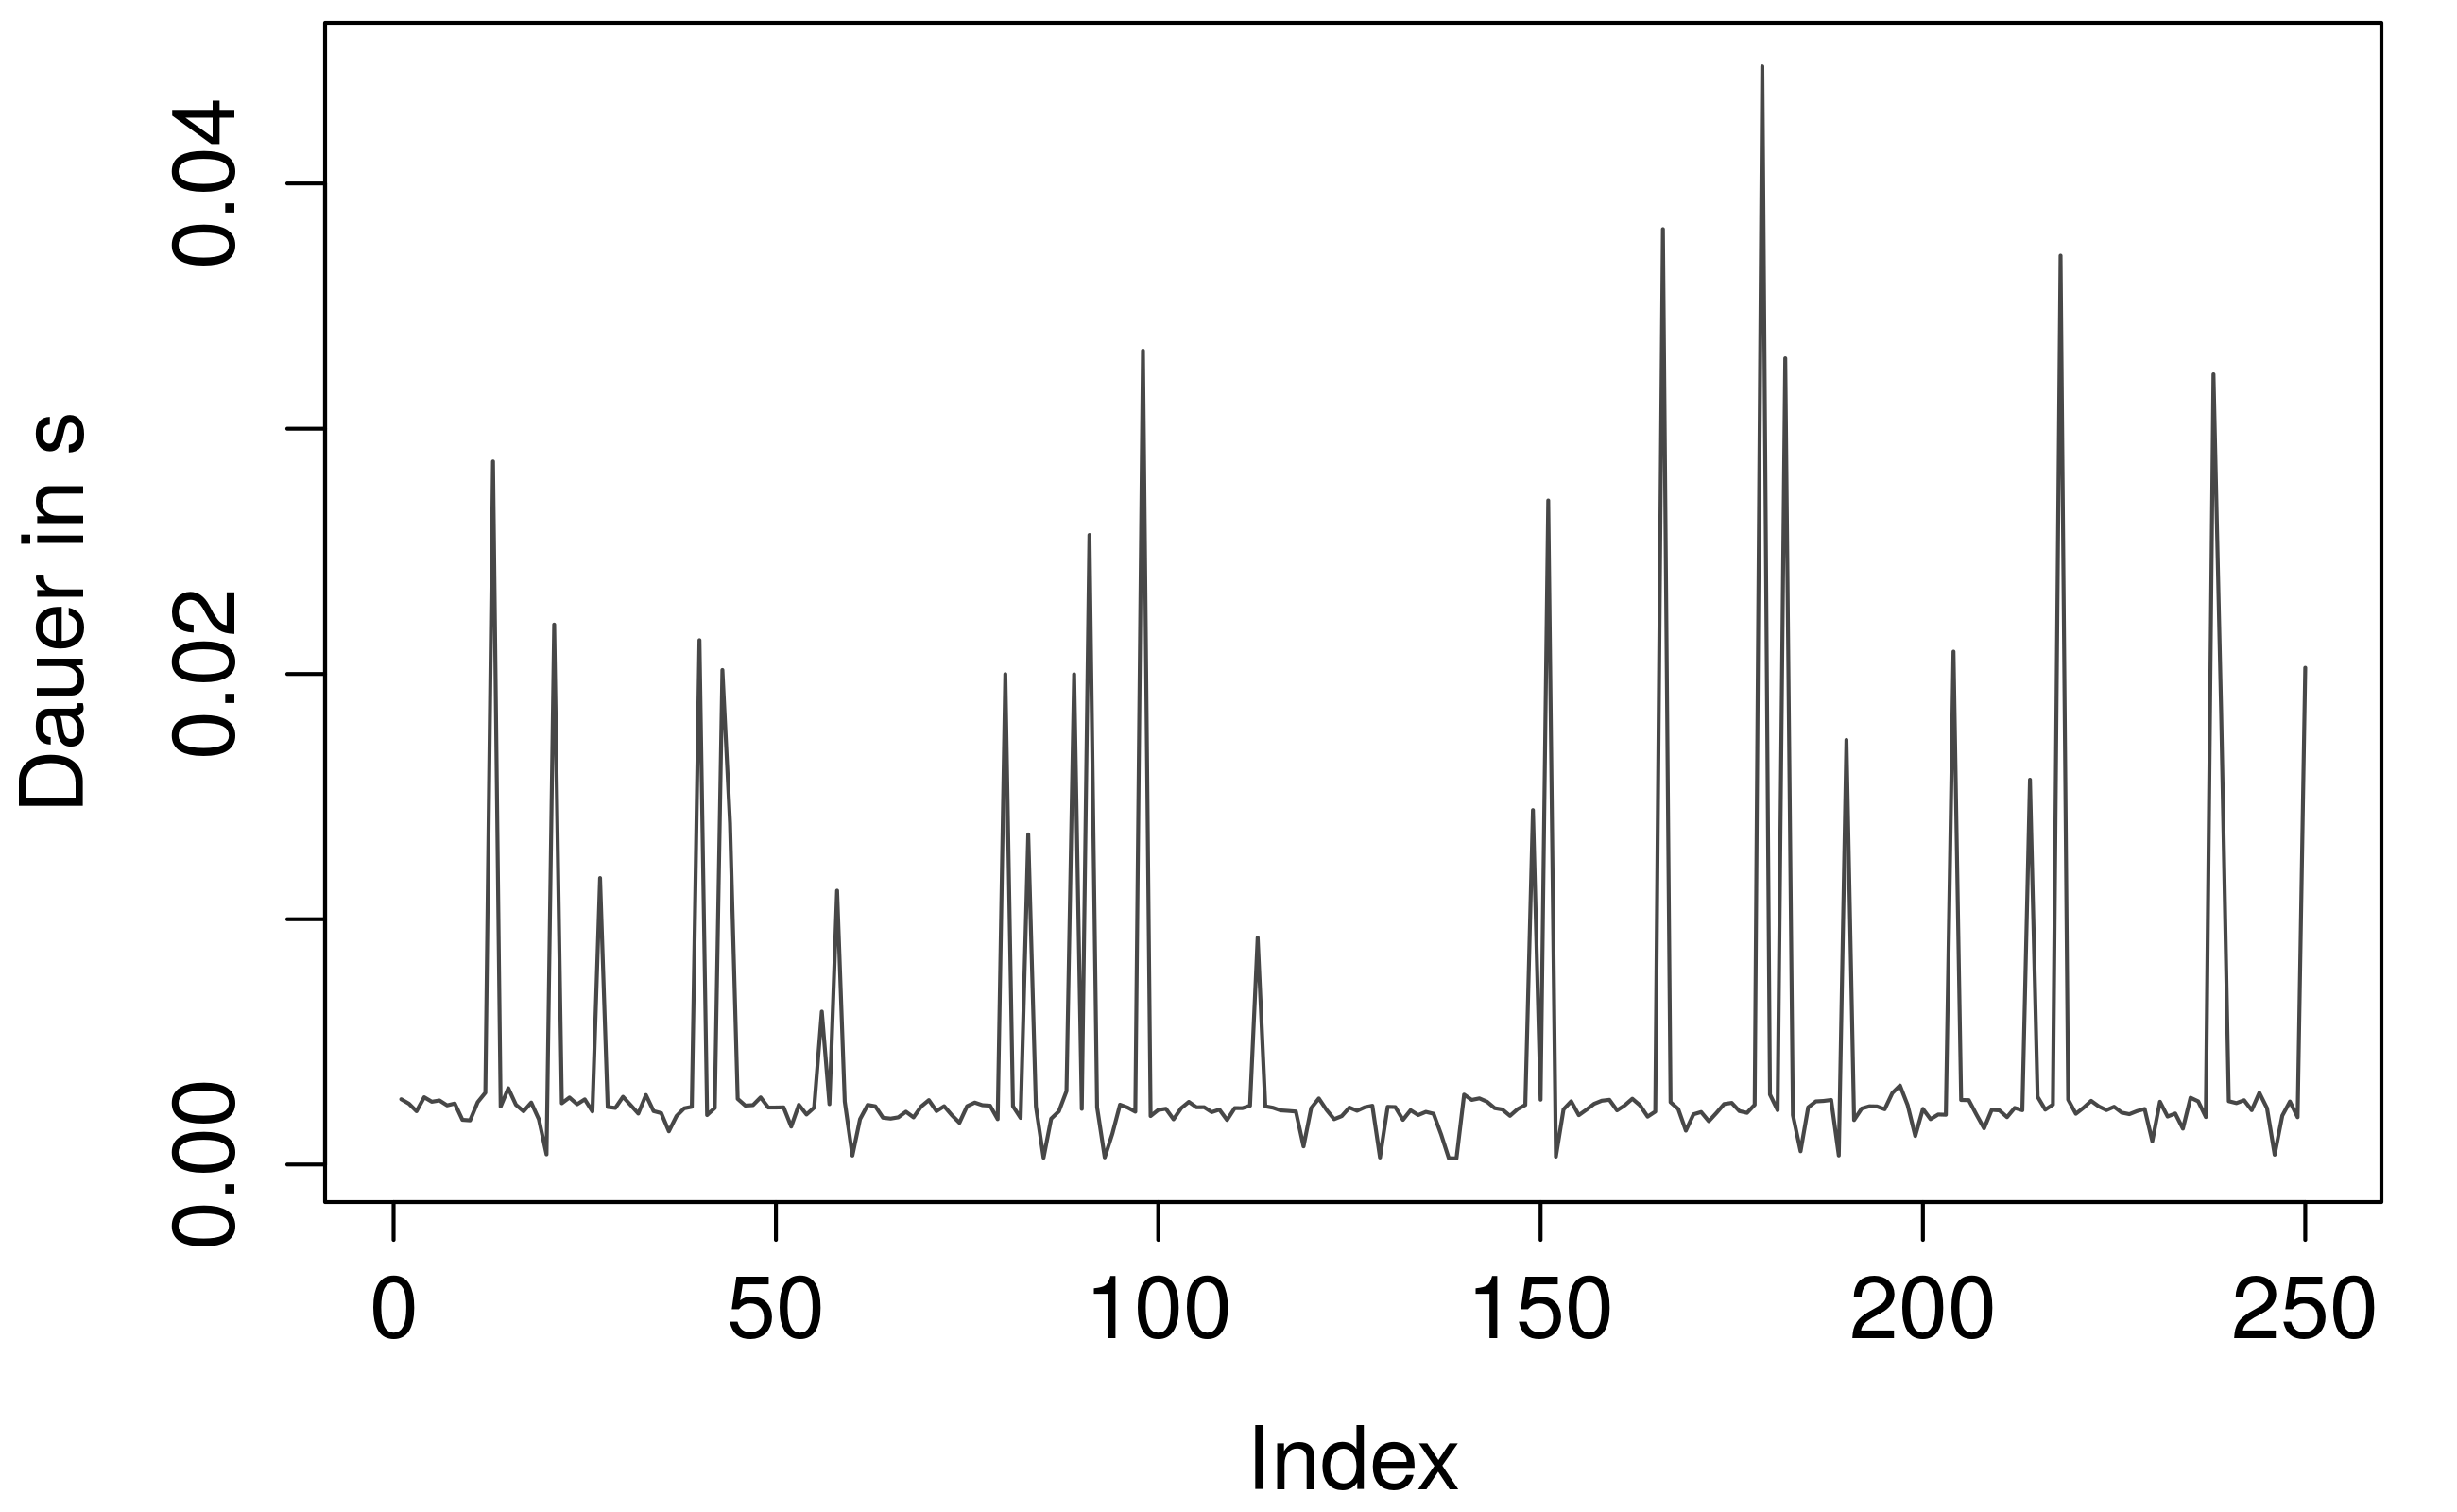
\includegraphics[width=.43\textwidth]{Bilder/Plots/exploration/plot_First250_read_rnd.png}
	}
	\hfill
	\subfloat[Randomisiert schreibend]{
		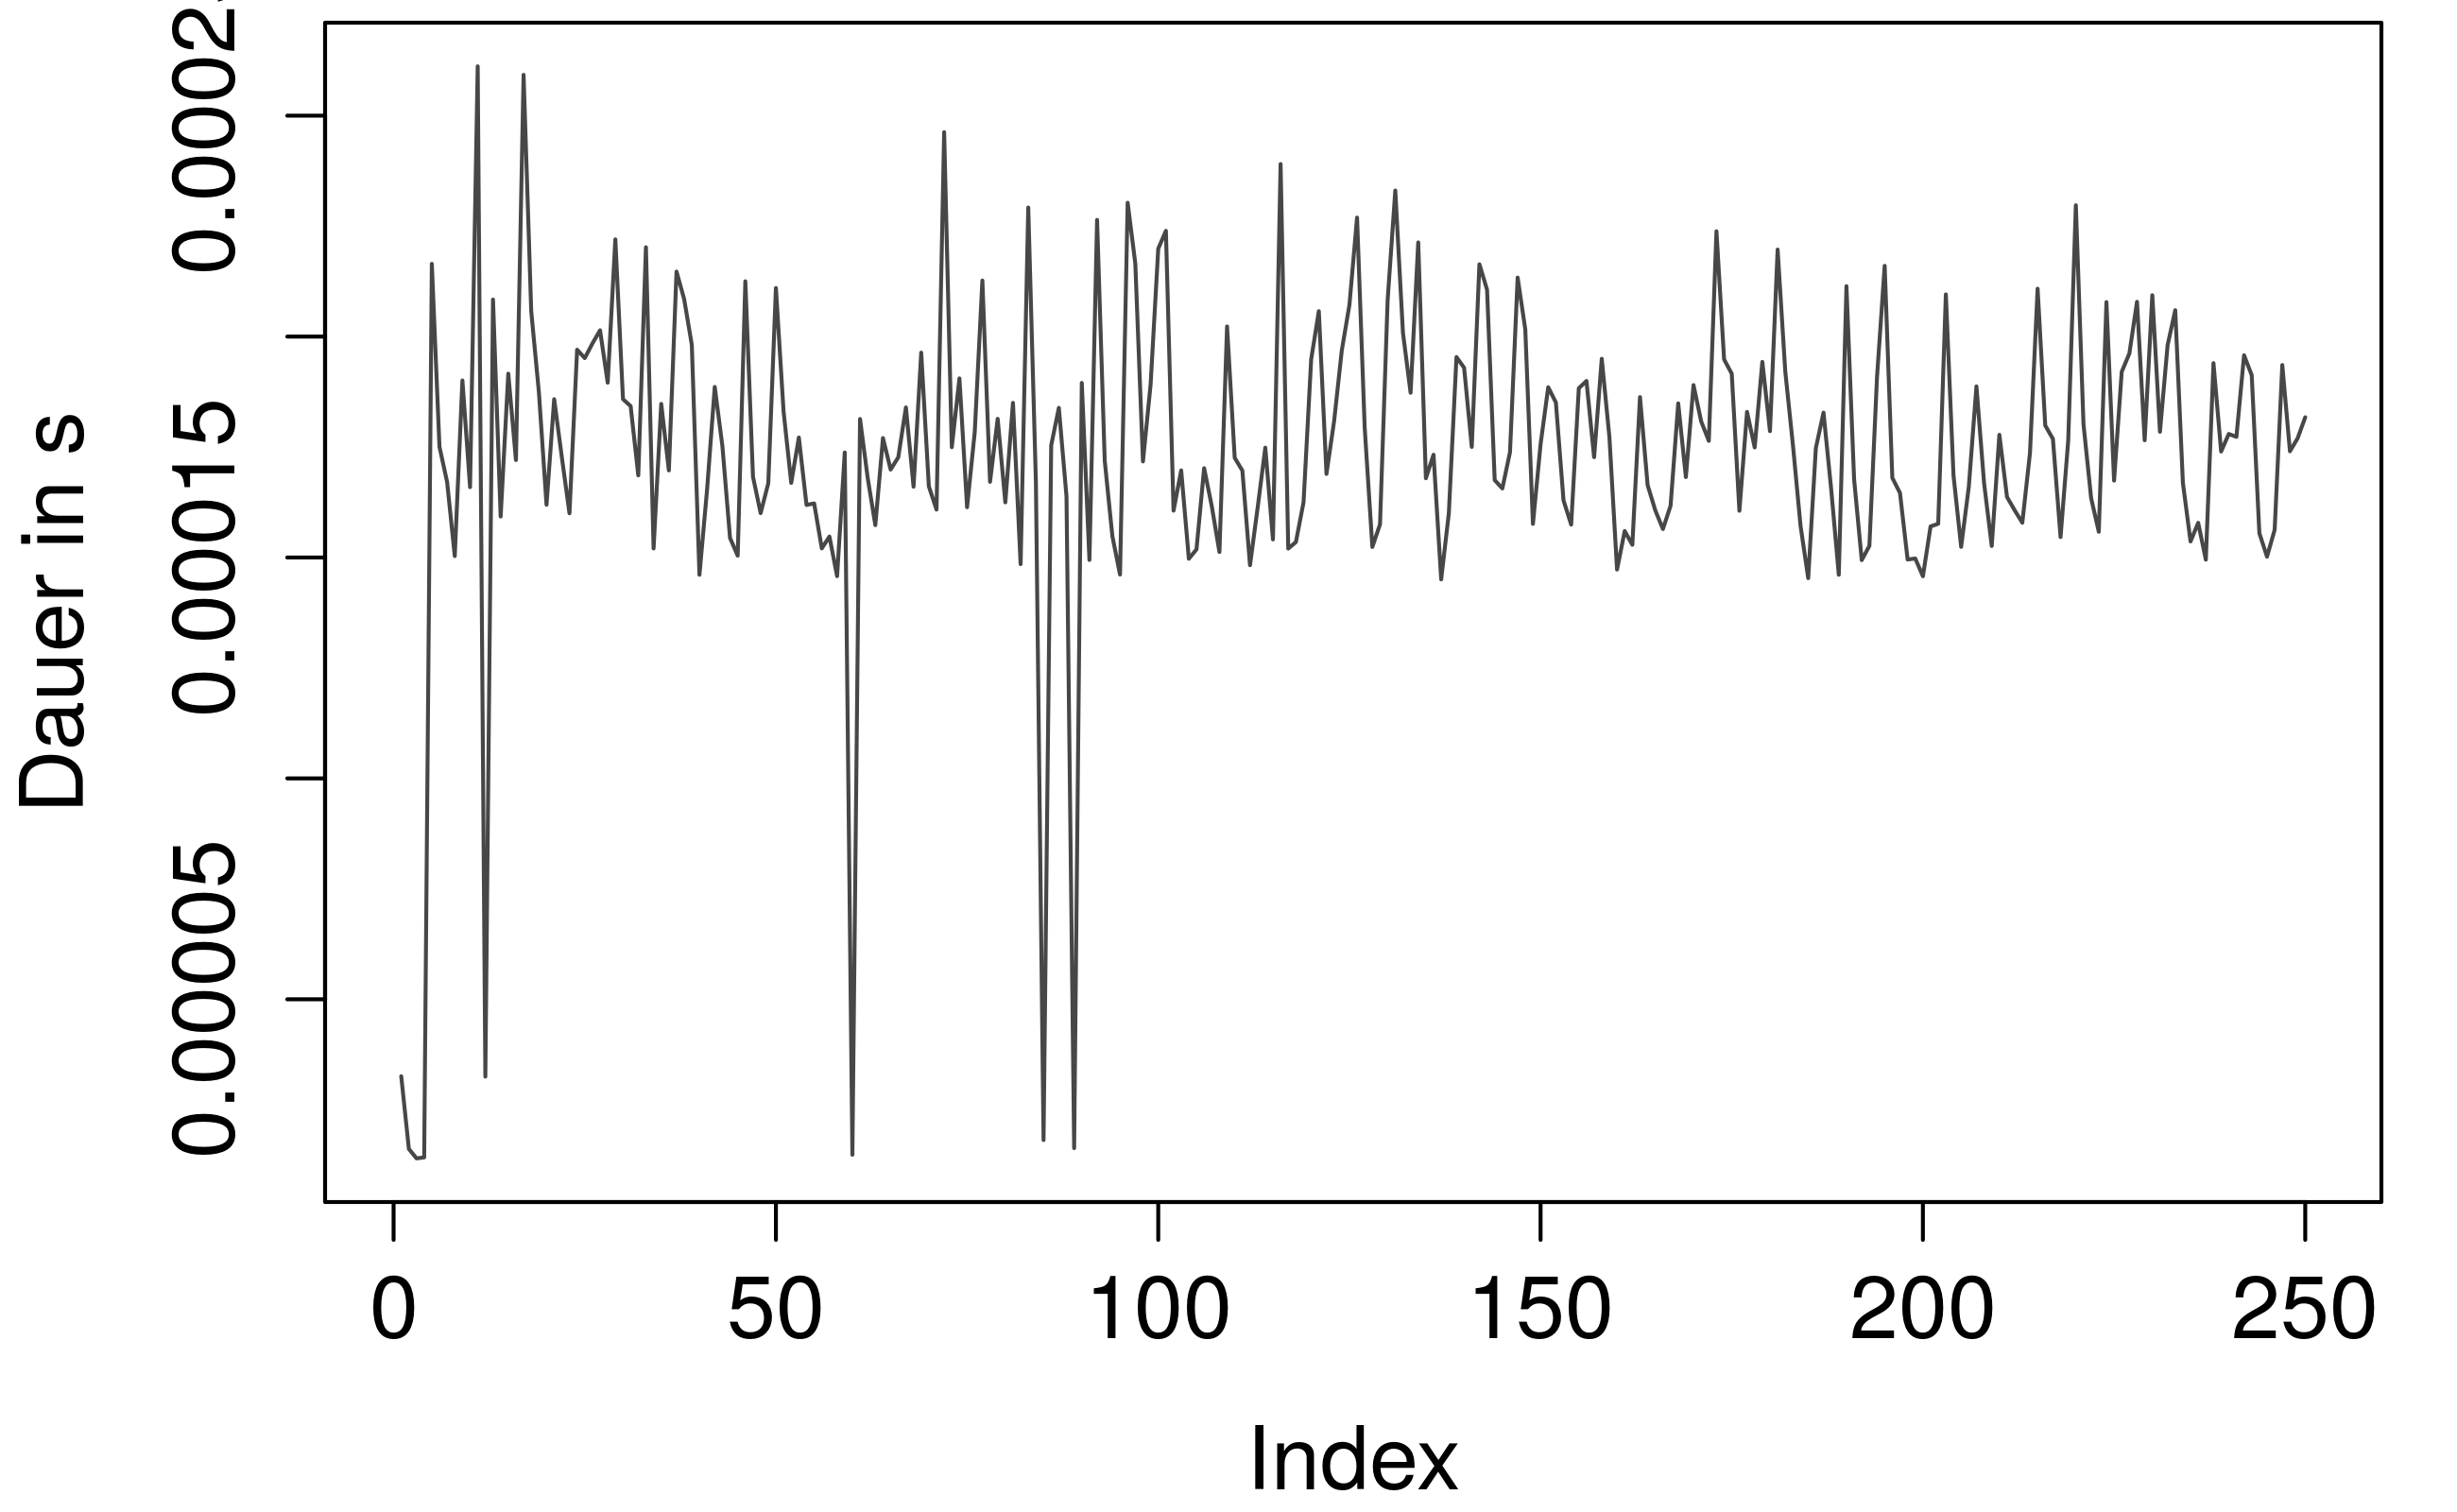
\includegraphics[width=.43\textwidth]{Bilder/Plots/exploration/plot_First250_write_rnd.png}
	}		
	\caption{Detailbetrachtung der ersten 250 Messungen}
	\label{fig:first250}
\end{figure} 

\begin{figure}
	\subfloat{
		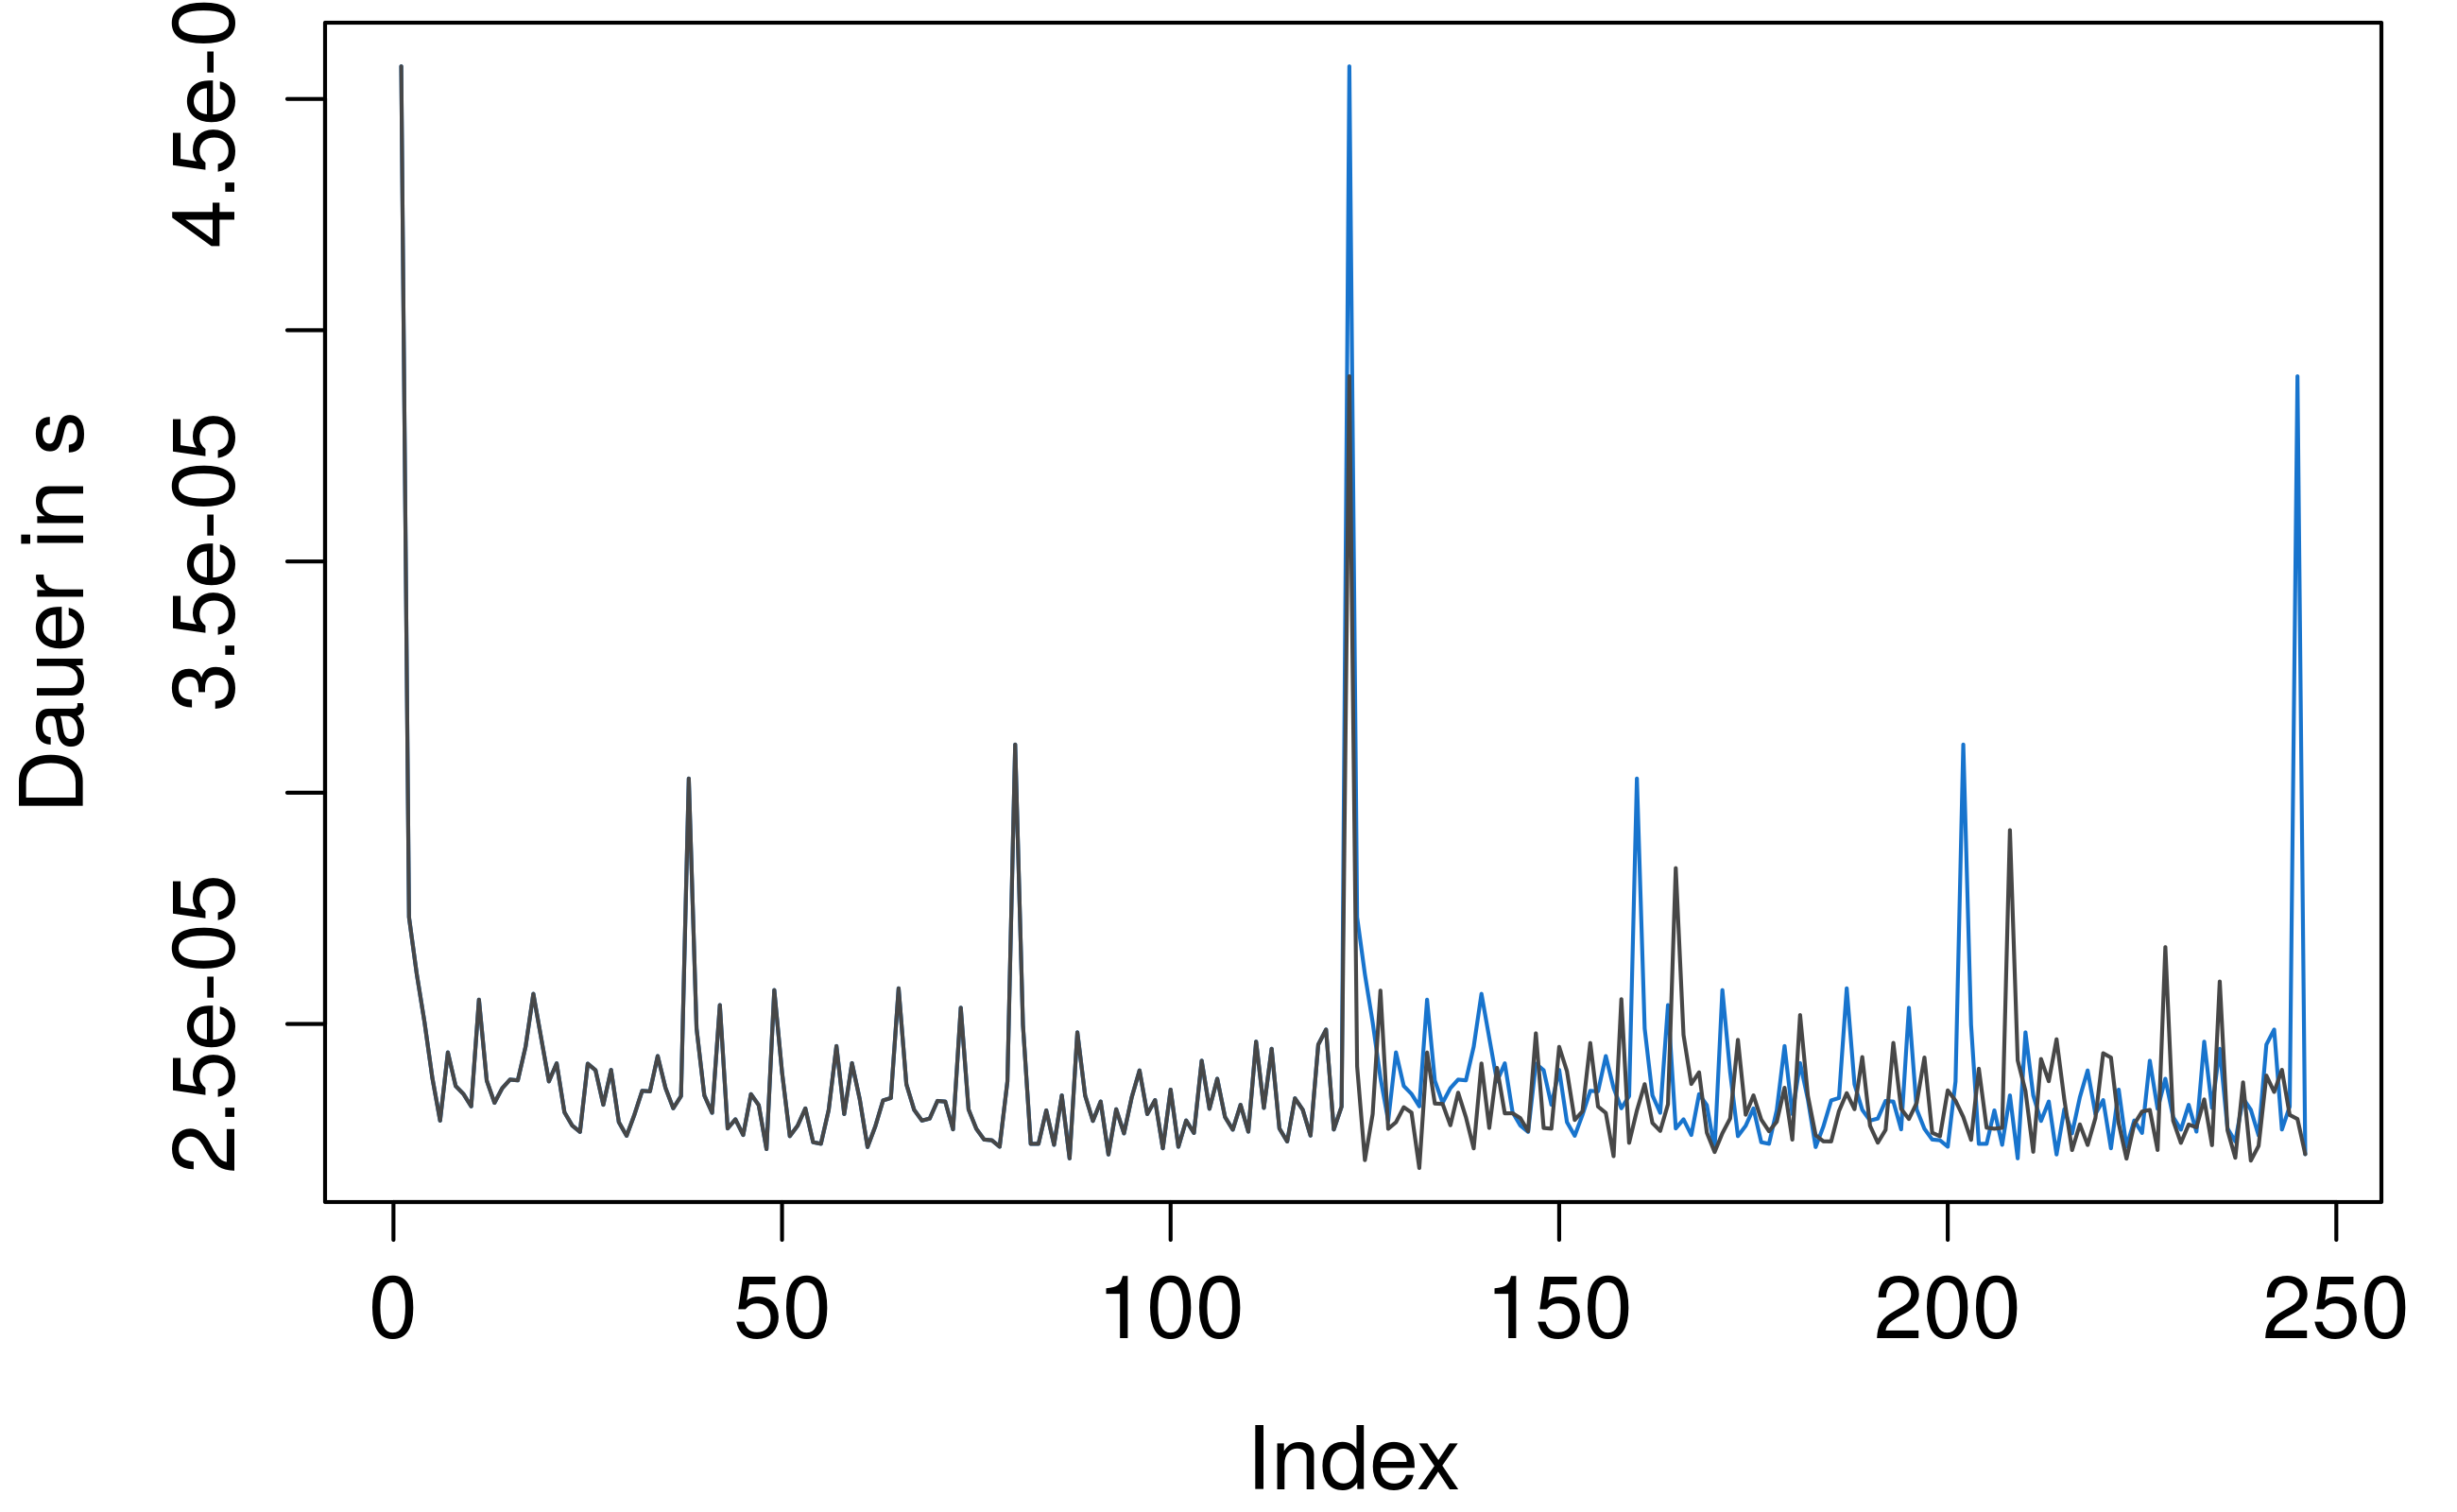
\includegraphics[width=0.9\textwidth]{Bilder/Plots/exploration/plot_periodicitywrite_seq.png}
	}	
	\caption{Wiederholung der ersten Werte der sequentiell schreibenden Messungen, als erstes einfaches Modell}
	\label{fig:periodicity}
\end{figure} 

Eine weitere Detailbetrachtung mache ich bei den Messungen 30.001 bis 30.250 in \ref{fig:from100001}.
Hier scheint eine Periodizität bei seq-R vorhanden zu sein. Und wenn eine Überlappung wie zuvor durchgeführt wird (diesmal nach den ersten 129 Messungen), so erkennt man, dass dieses simple Modell die Ausreißer für diesen kleinen Ausschnitt exakt vorhersagen kann.
Im Allgemeinen kann dies jedoch offensichtlich nicht funktionieren.
Doch die Annahme einer gewissen Periodizität in der Leistung des E/A-Systems ist scheinbar gerechtfertigt. Ein Modell das versucht diese auszunutzen muss eine komplexere Methode als schlichtes Übertragen vorheriger Leistungswerte haben, ansonsten kann es wohl nur in äußerst eingeschränktem Maße korrekte Leistung vorhersagen.

\begin{figure}
	\subfloat[Sequentiell lesend]{
		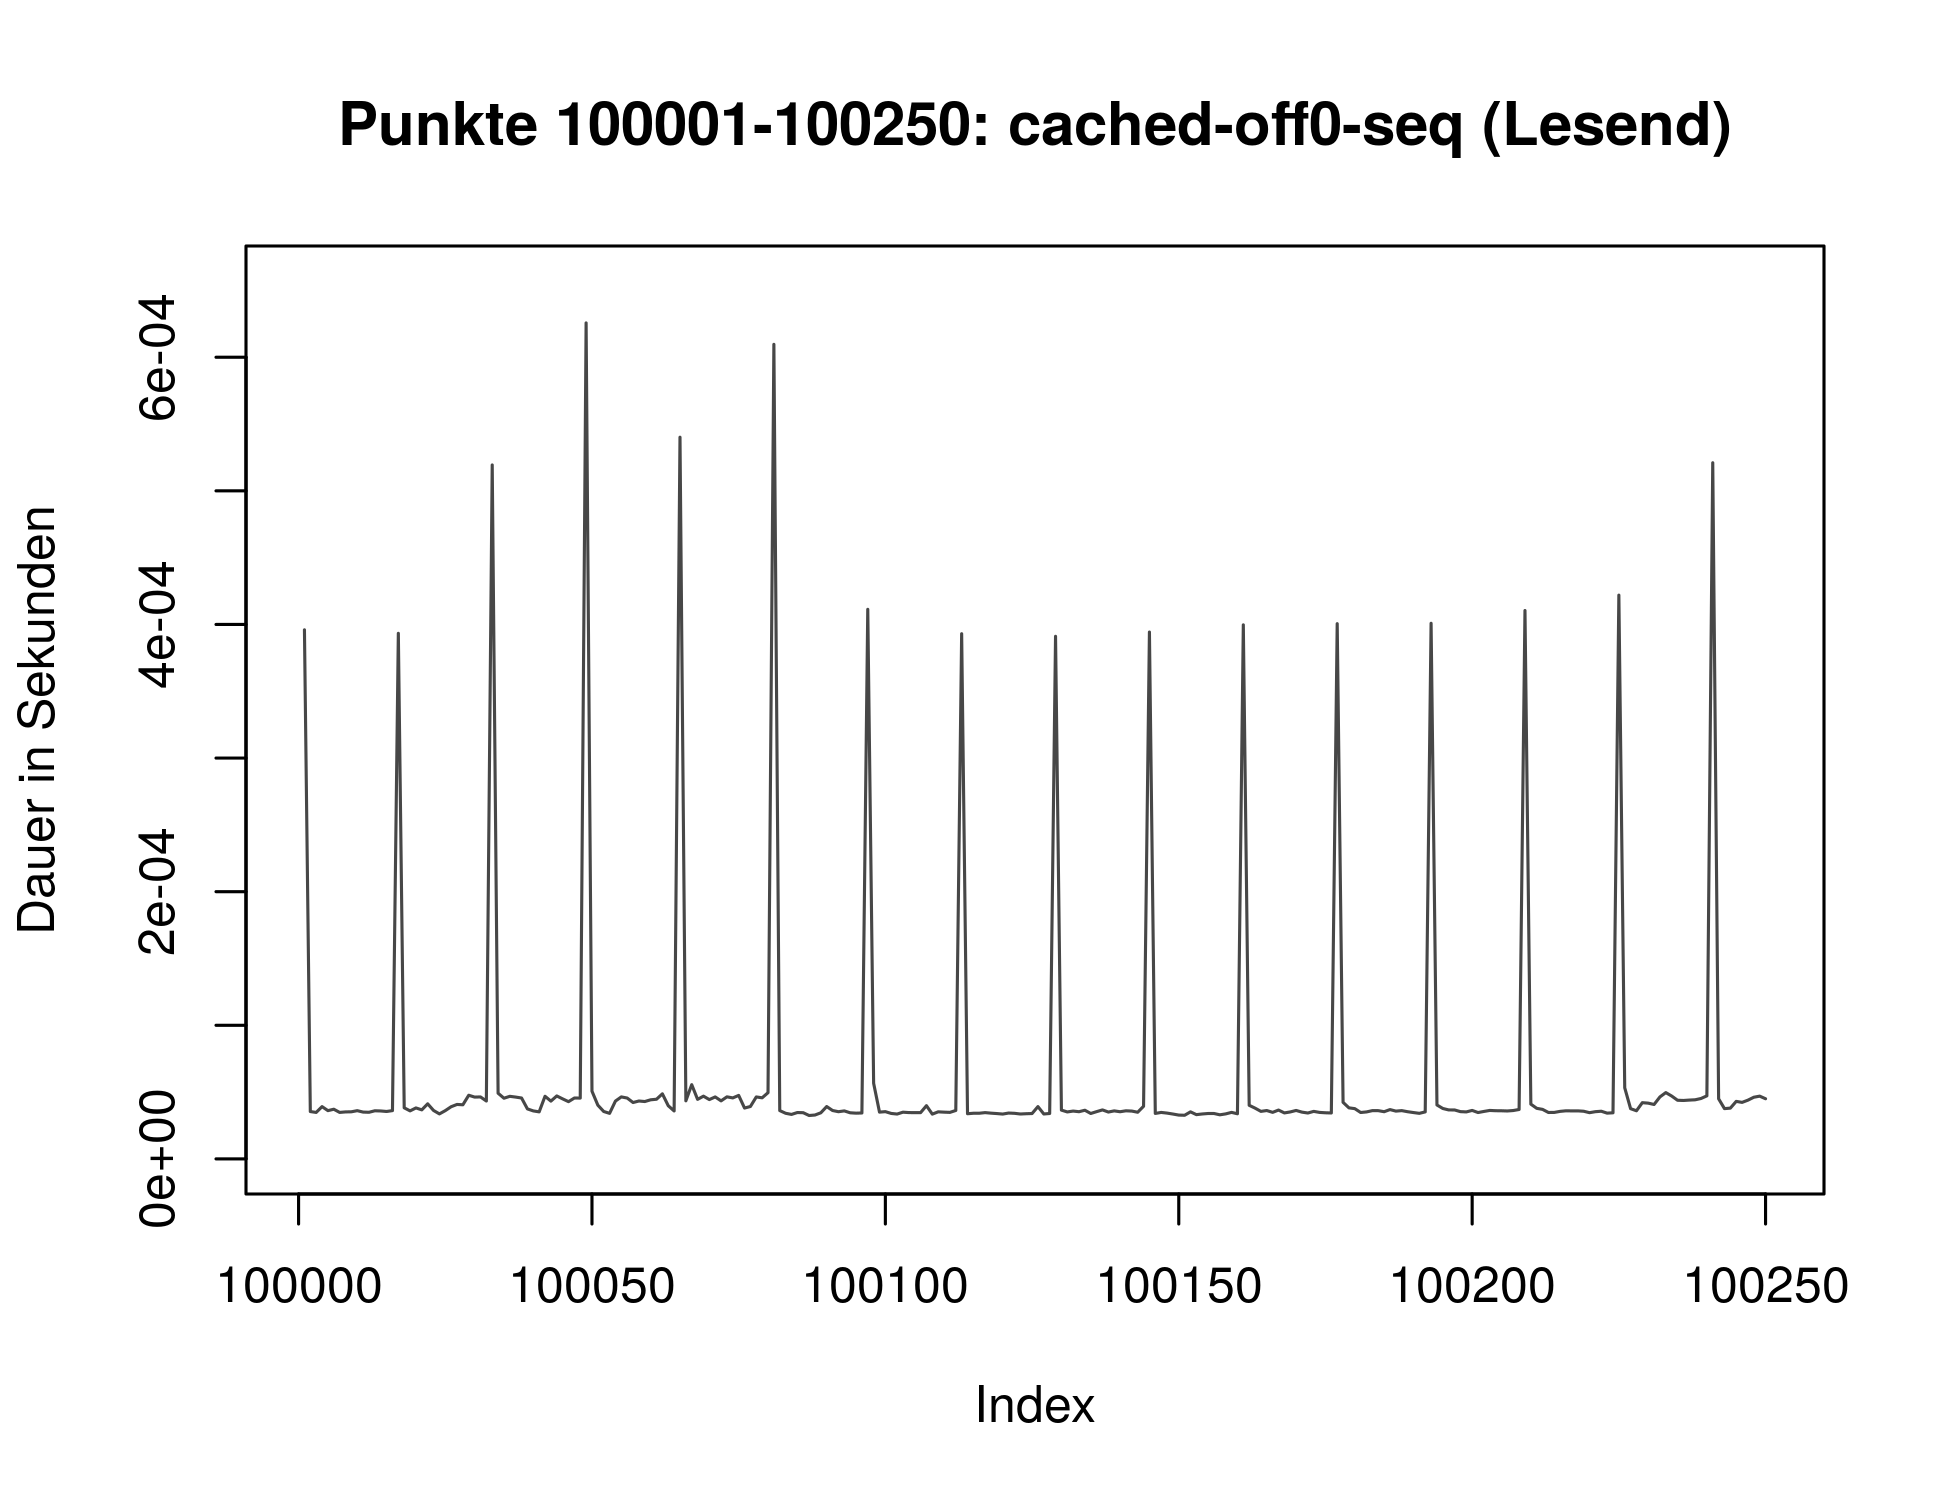
\includegraphics[width=.43\textwidth]{Bilder/Plots/exploration/plot_From100001to100250_read_seq.png}
	}
	\hfill
	\subfloat[Sequentiell schreibend]{
		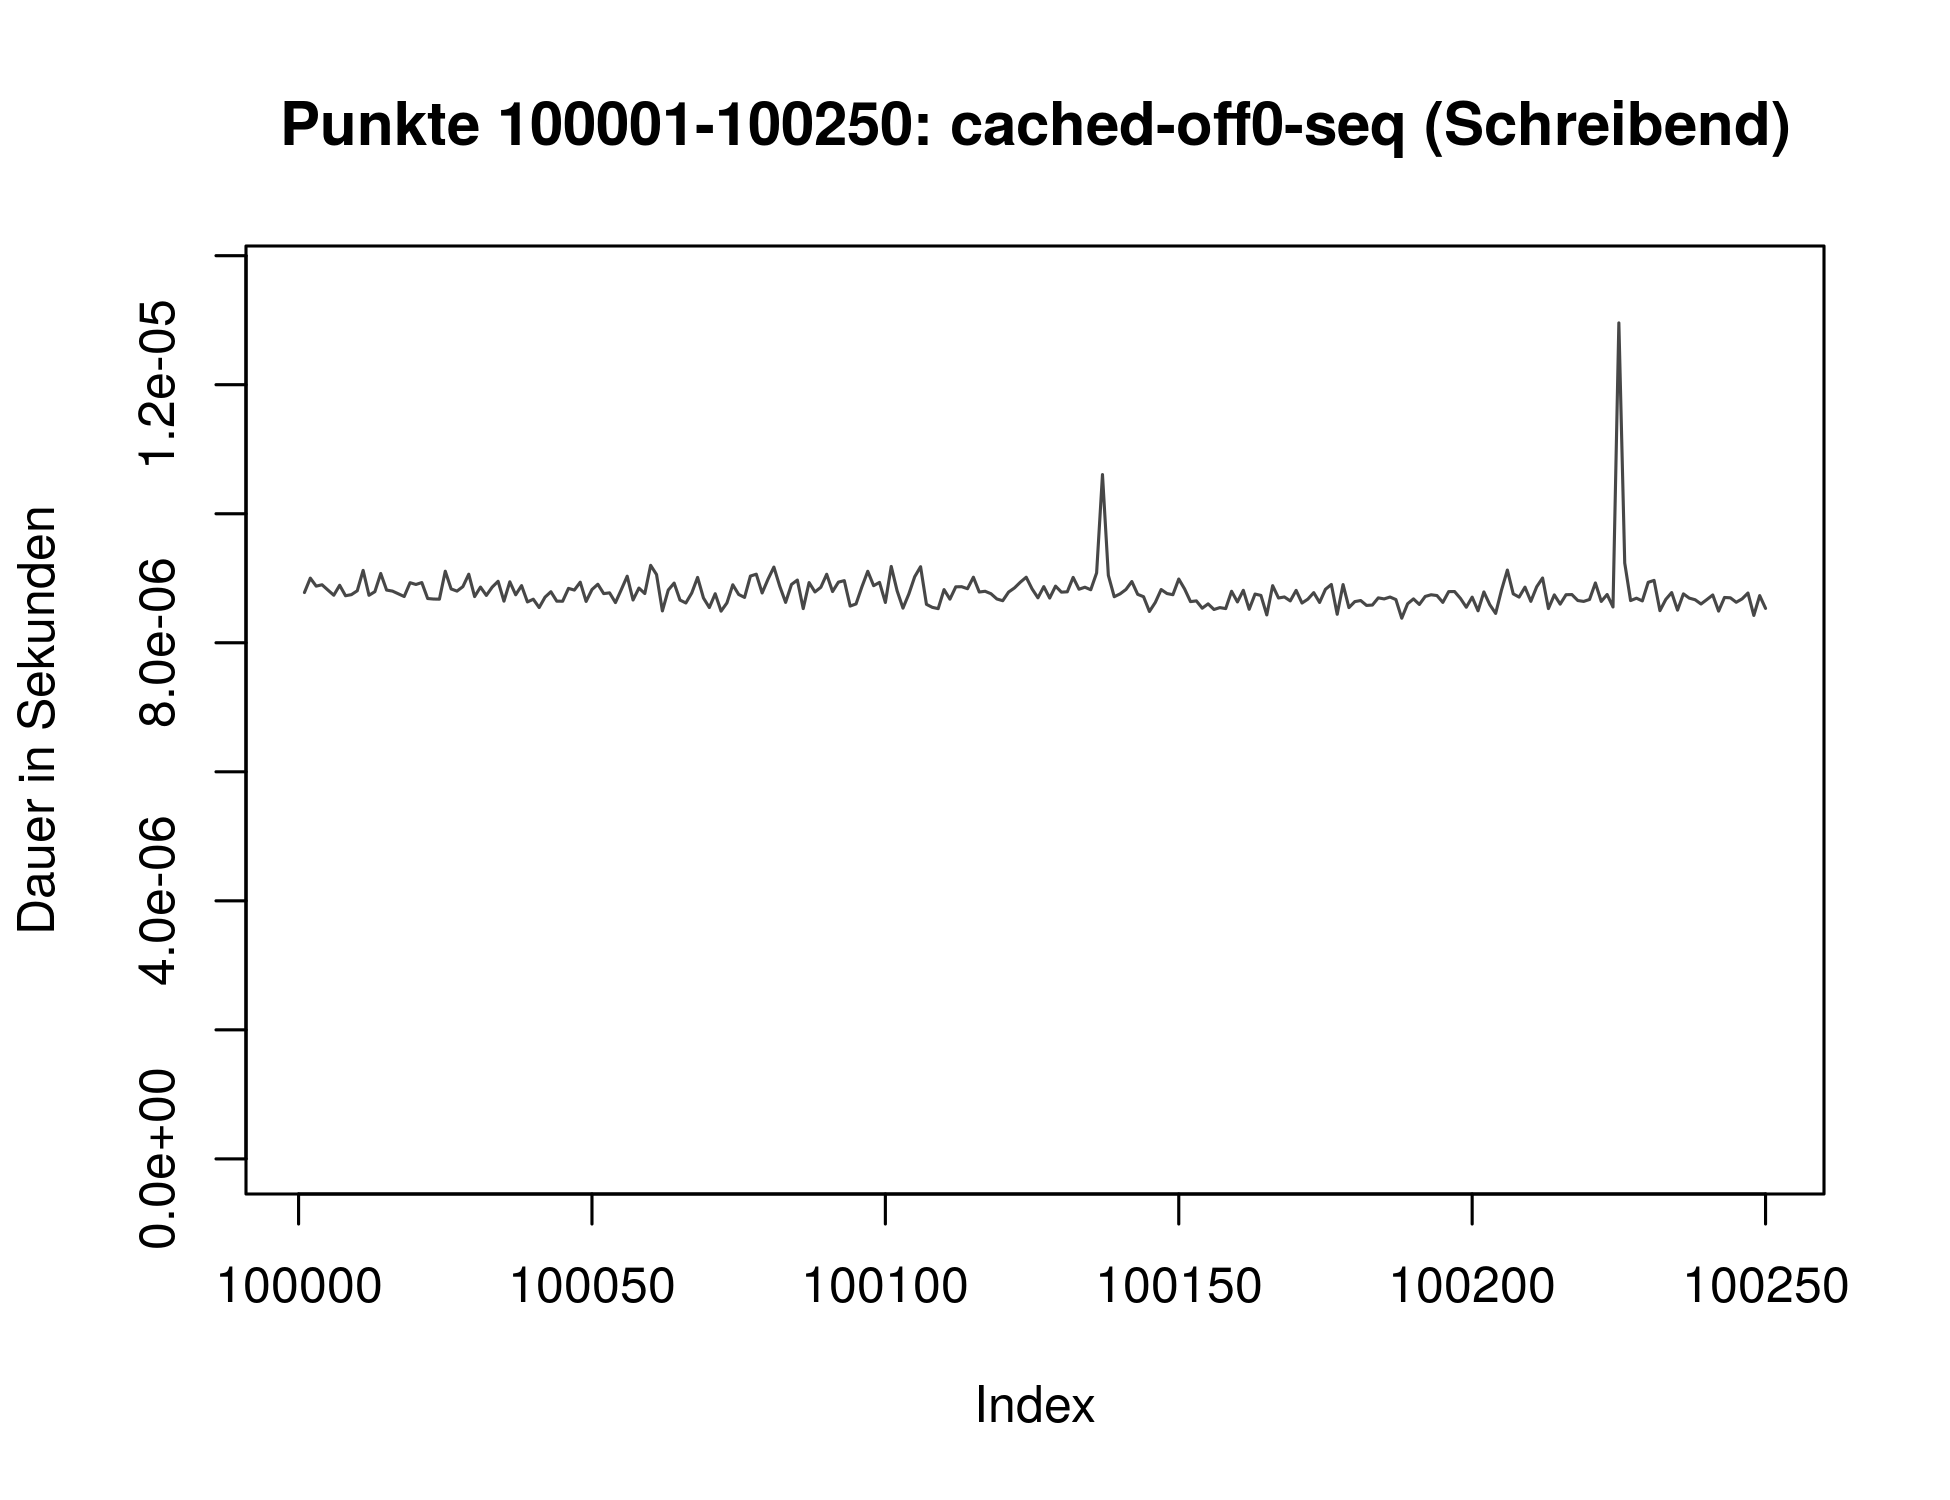
\includegraphics[width=.43\textwidth]{Bilder/Plots/exploration/plot_From100001to100250_write_seq.png}
	}\\
	\subfloat[Randomisiert lesend]{
		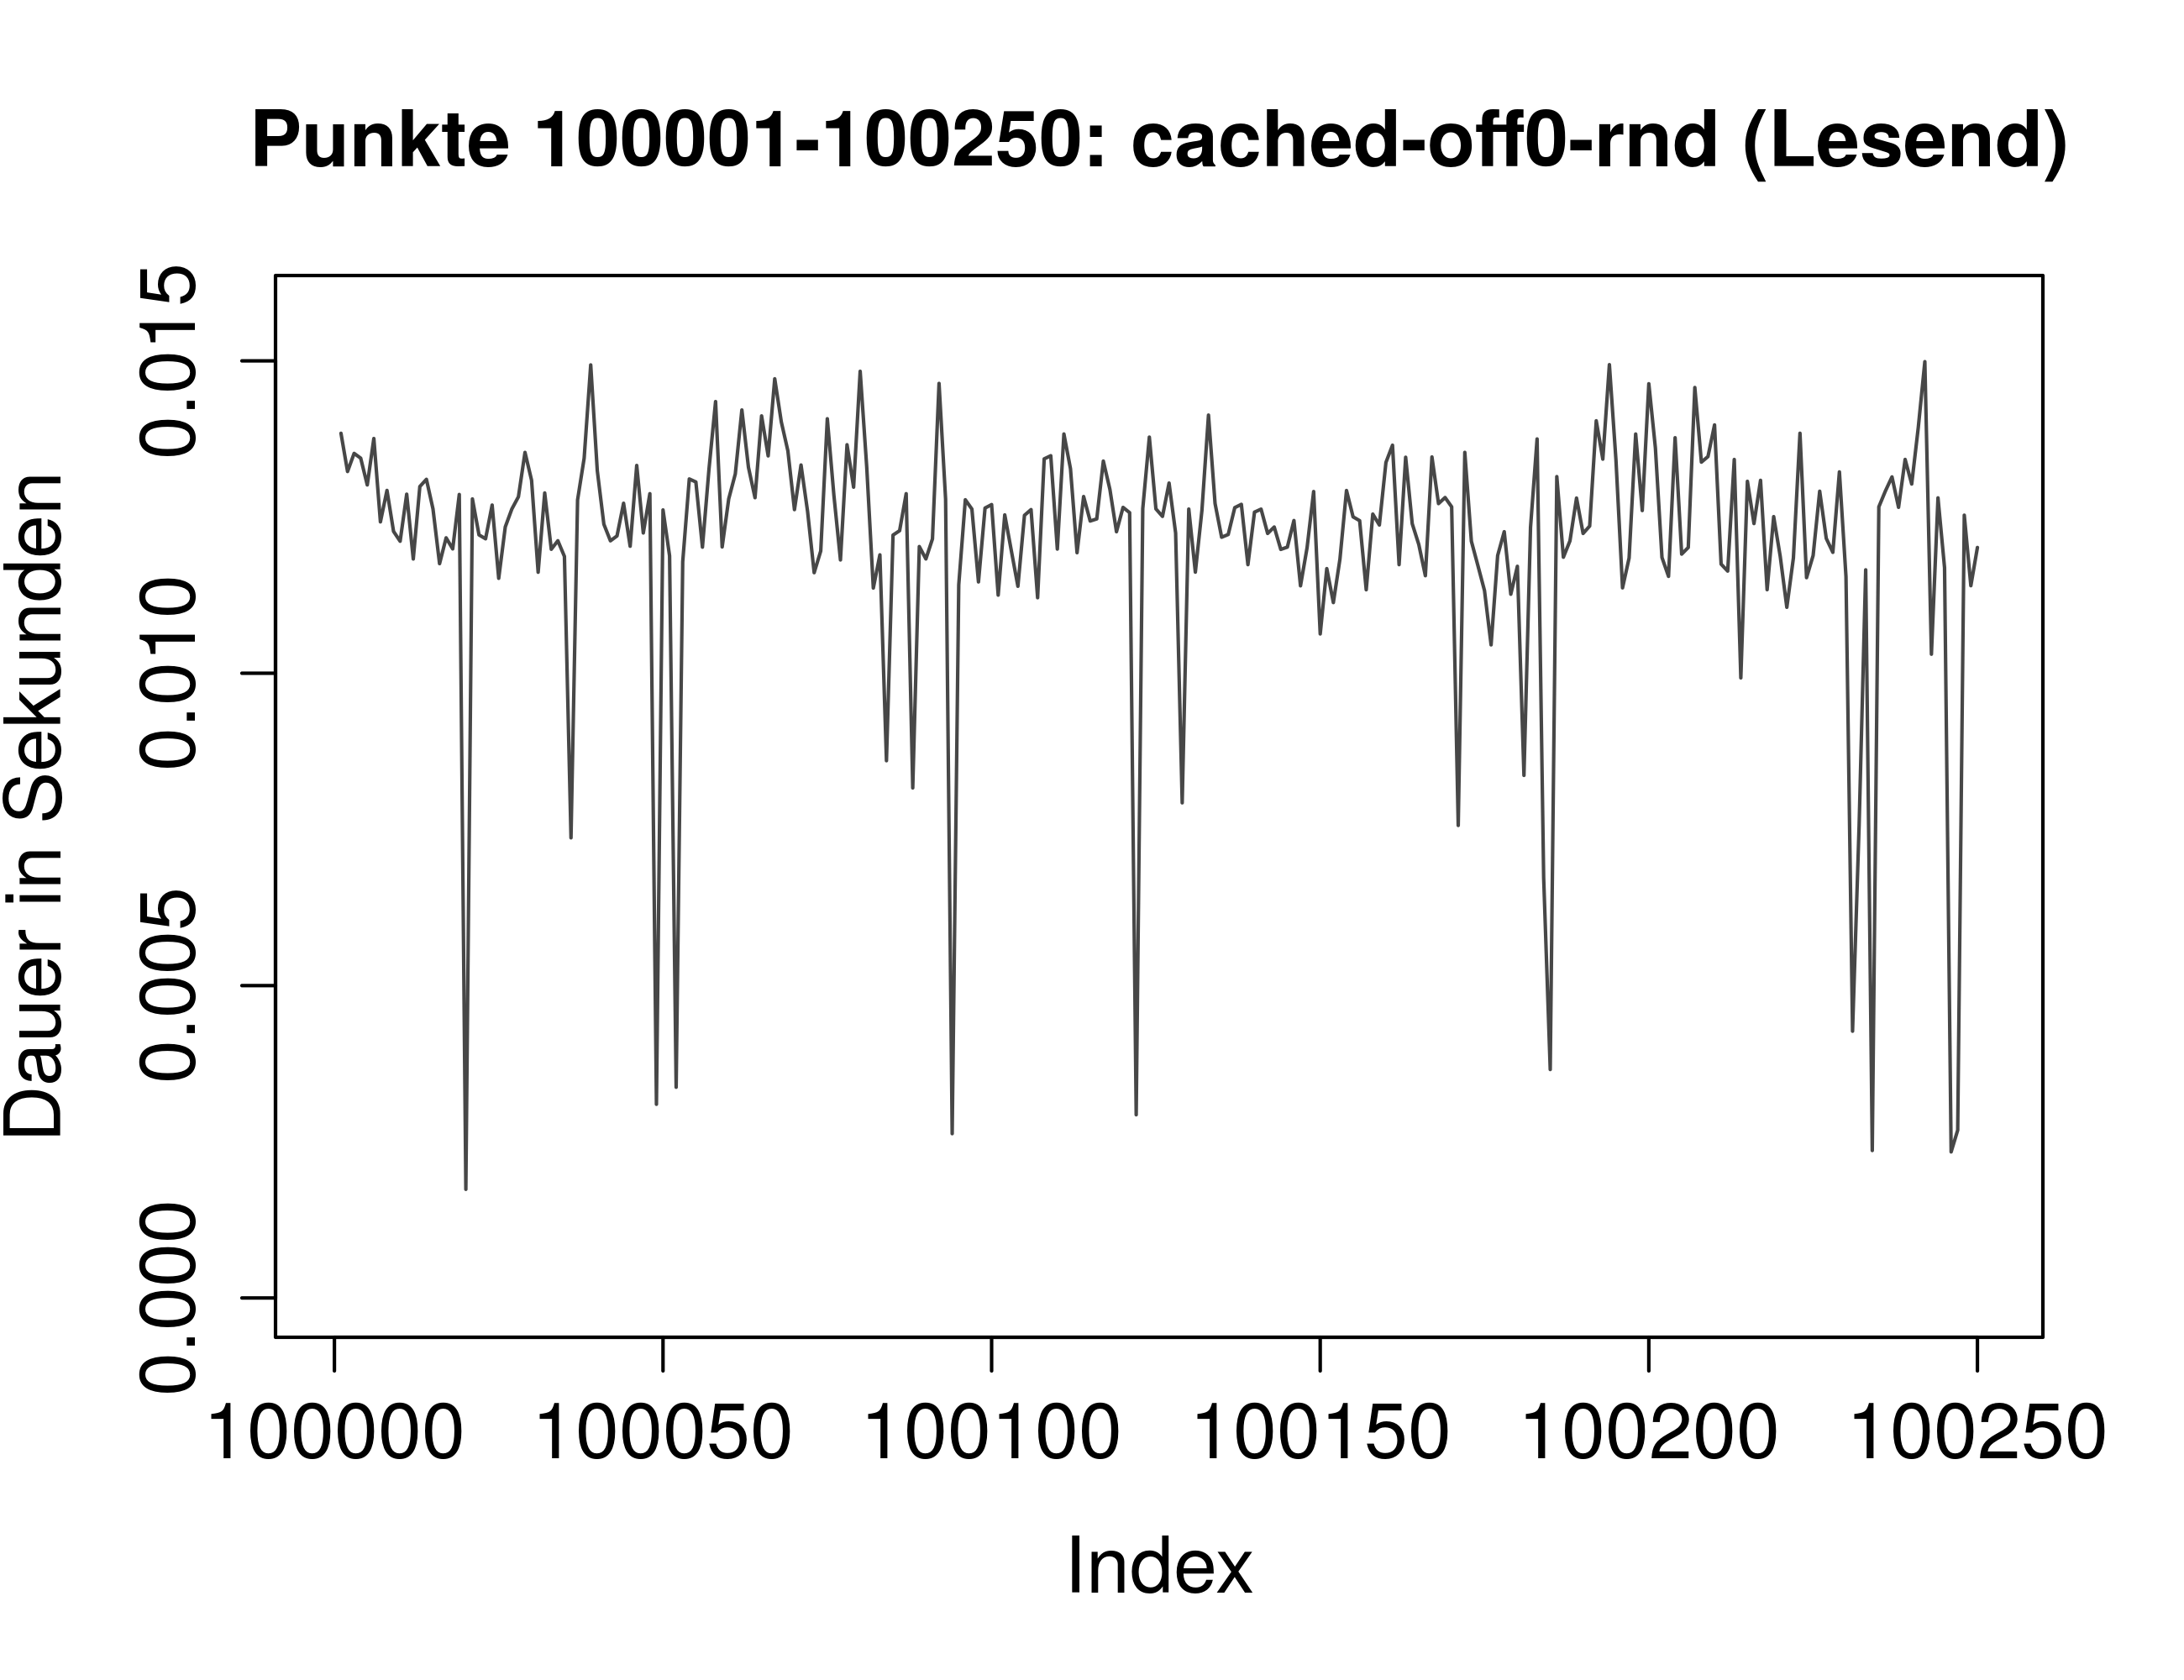
\includegraphics[width=.43\textwidth]{Bilder/Plots/exploration/plot_From100001to100250_read_rnd.png}
	}
	\hfill
	\subfloat[Randomisiert schreibend]{
		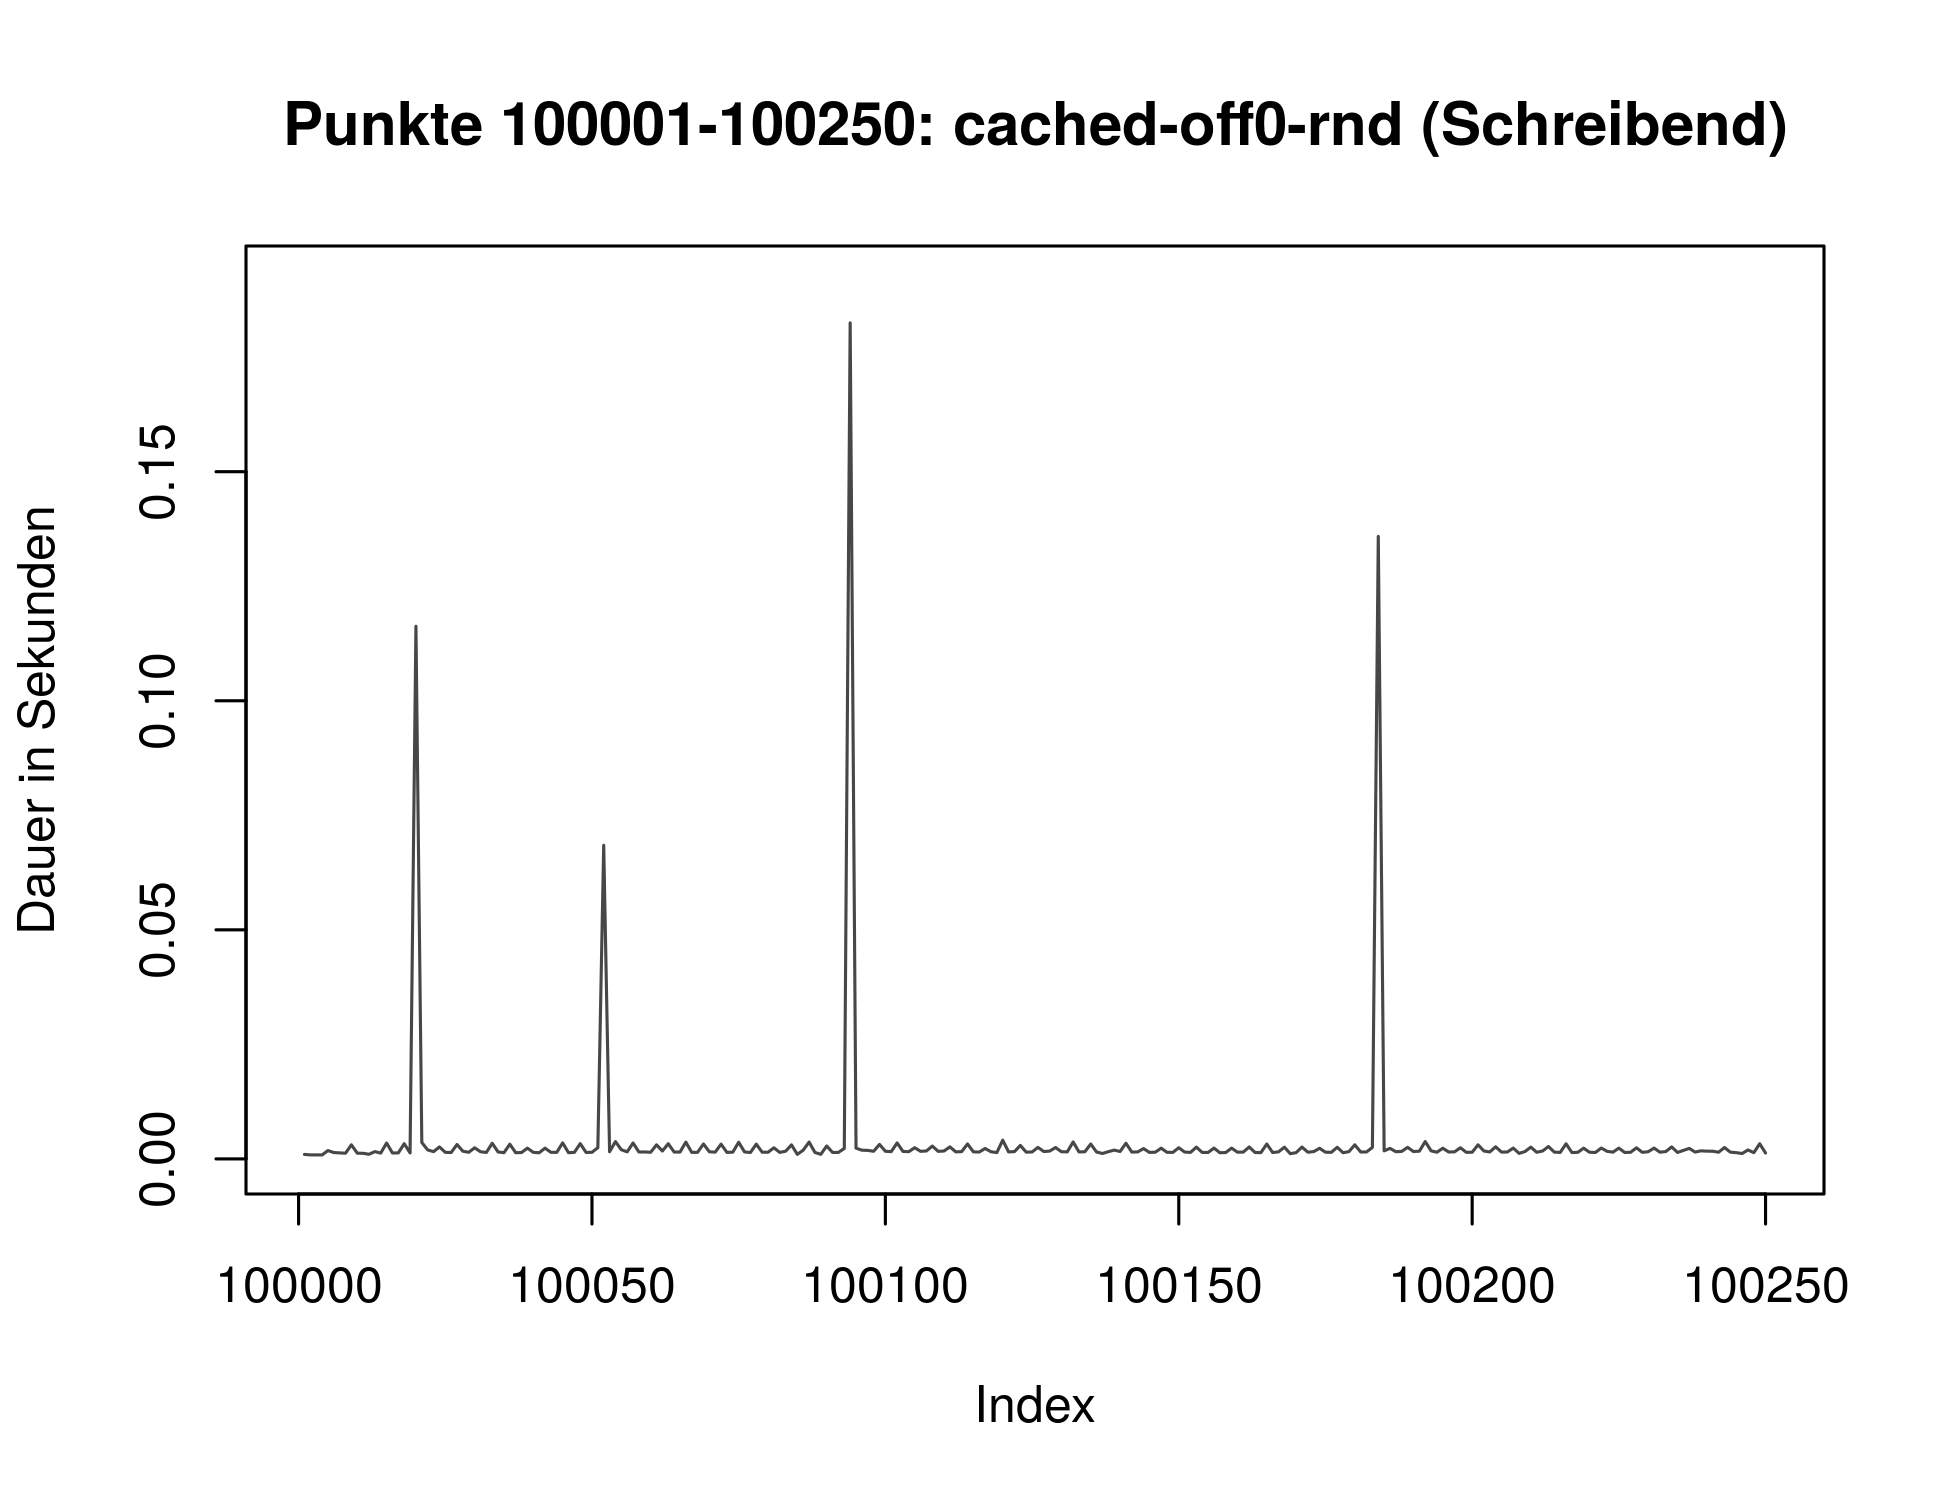
\includegraphics[width=.43\textwidth]{Bilder/Plots/exploration/plot_From100001to100250_write_rnd.png}
	}		
	\caption{Detailbetrachtung der Messungen 100001 bis 100250}
	\label{fig:from100001}
\end{figure} 

\begin{figure}
	\subfloat{
		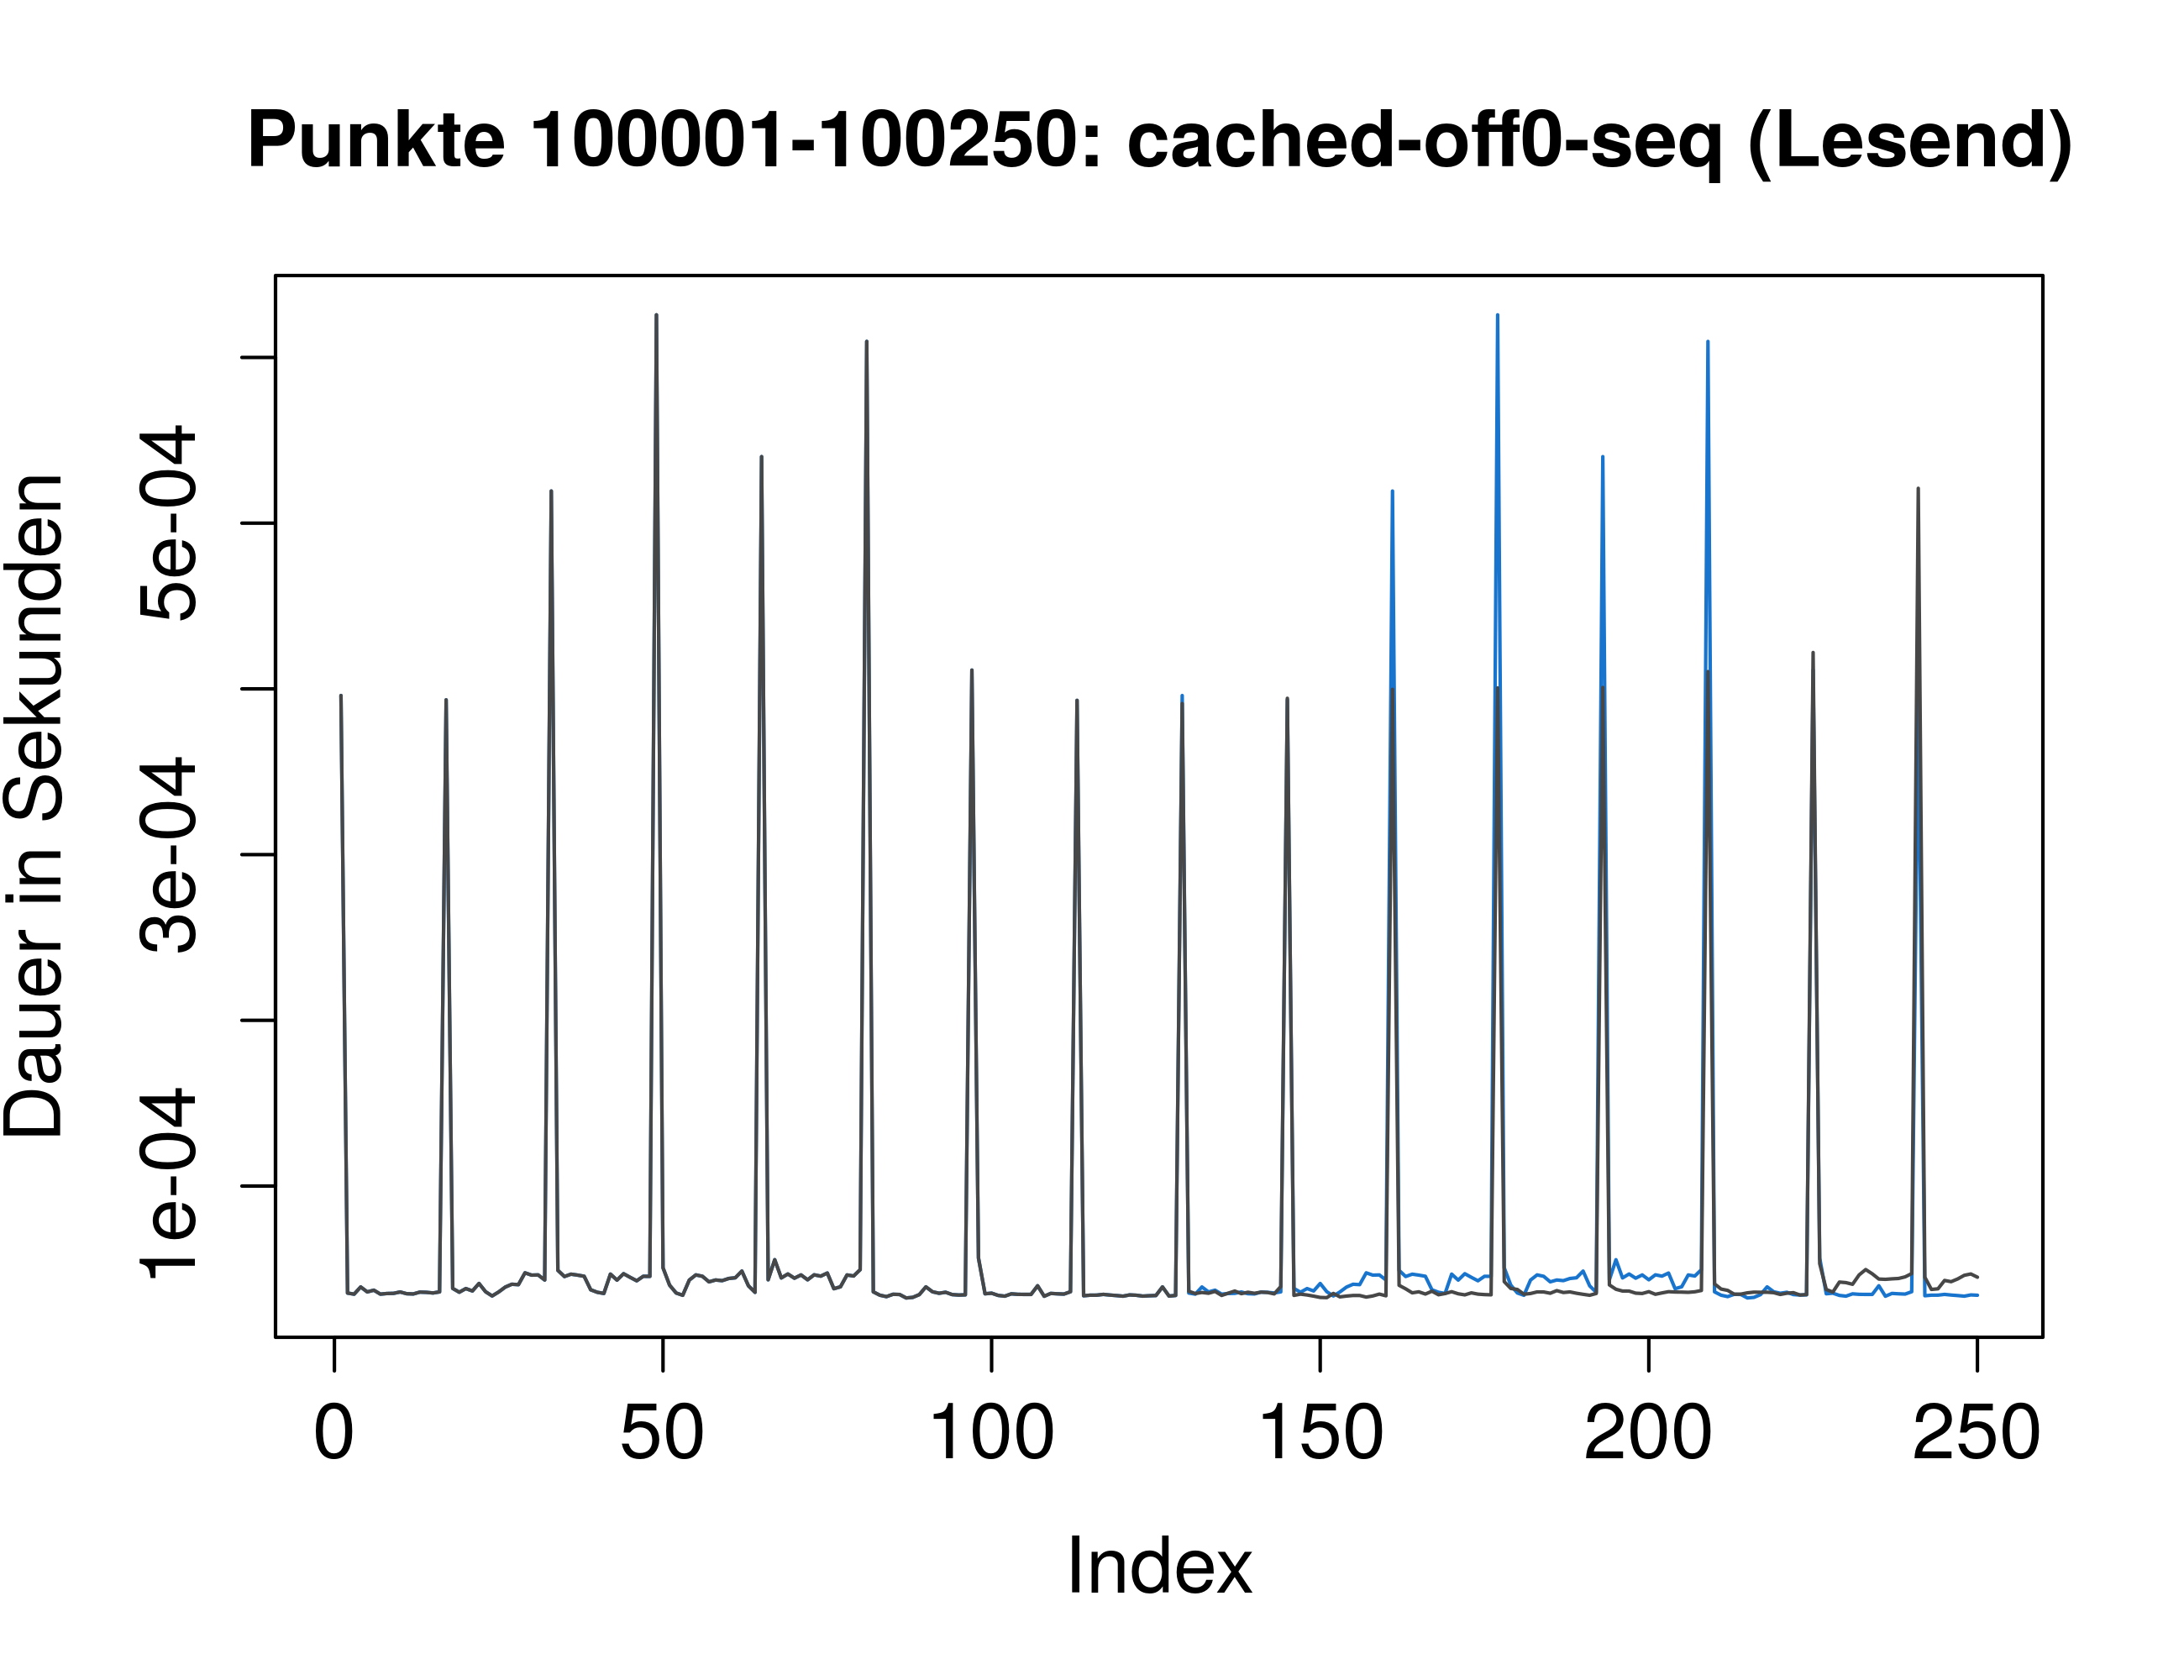
\includegraphics[width=.9\textwidth]{Bilder/Plots/exploration/plot_periodicity100001read_seq.png}
	}	
	\caption{Wiederholung der ersten Werte der sequentiell lesenden Messungen, als erstes einfaches Modell}
	\label{fig:periodicity100001}
\end{figure} 
\clearpage

\section{Analyse der Fehlerklassen}
\label{fk_analyse}
Alle Modelle werden auf den zusammengeführten Datensätzen aus lesenden und schreibenden Zugriffen angewendet. Daher gibt es im folgenden nur noch jeweils eine Abbildung zu den sequentiellen und eine zu den Messungen mit zufälligem Dateizugriff.
Zunächst werden alle Daten der Messreihen zu einer Zugriffsgröße mit lesenden Aufrufen gezeichnet, danach kommen die schreibenden Zugriffe. 
Die in \ref{fk-modelle} eingeführten Fehlerklassen untersuche ich anhand der Ergebnisse, die aus der Clusteranalyse des Residuums von \textit{LinReg G} entstanden sind.
In \ref{fig:error_class_clustering_seq}a, sowie \ref{fig:error_class_clustering_rnd}a ist in Zeitreihe der Fehler aufgezeichnet, den \textit{LinReg G} auf den sequentiell, respektive randomisiert ausgeführten Messungen, mit seinen Vorhersagen gegenüber den tatsächlichen Laufzeiten gemacht hat.

Interessanterweise ist die Modellabweichung auf den sequentiellen Daten im Wesentlichen unabhängig vom Operationstyp, während auf den randomisierten Daten größere Fehler bei lesenden Aufrufen gemacht werden.
Die absolute Abweichung wächst bei sequentiellen Zugriff mit der Größe der E/A-Aufrufe, für die zufälligen Zugriffe gilt dies nur bedingt. Auf den kleinsten Zugriffsgrößen werden kleine Fehler gemacht, danach bleibt der Betrag in etwa auf einem Niveau.
Ein Grund für höhere Abweichungen bei aufwendigeren Messungen ist, dass ein bestimmter relativer Fehler zu entsprechend höheren absoluten Fehlern führt.
Wegen dem plötzlichen und sehr starken Anstieg der Residuen für die höchsten Zugriffsgrößen kann dies nicht die einzige Erklärung sein.
Ein weiterer Grund könnte sein, dass die E/A-Leistung in den Bereichen mit höheren Zugriffsgrößen eine höhere Varianz aufweist und somit unberechenbarer wird.

\begin{figure}
	\centering
	\subfloat[Sortiert nach Zugriffsgröße in $\text{}$ dunkelgrau lesende und in hellgrau schreibende Zugriffe, begrenzte Y-Achse]{
		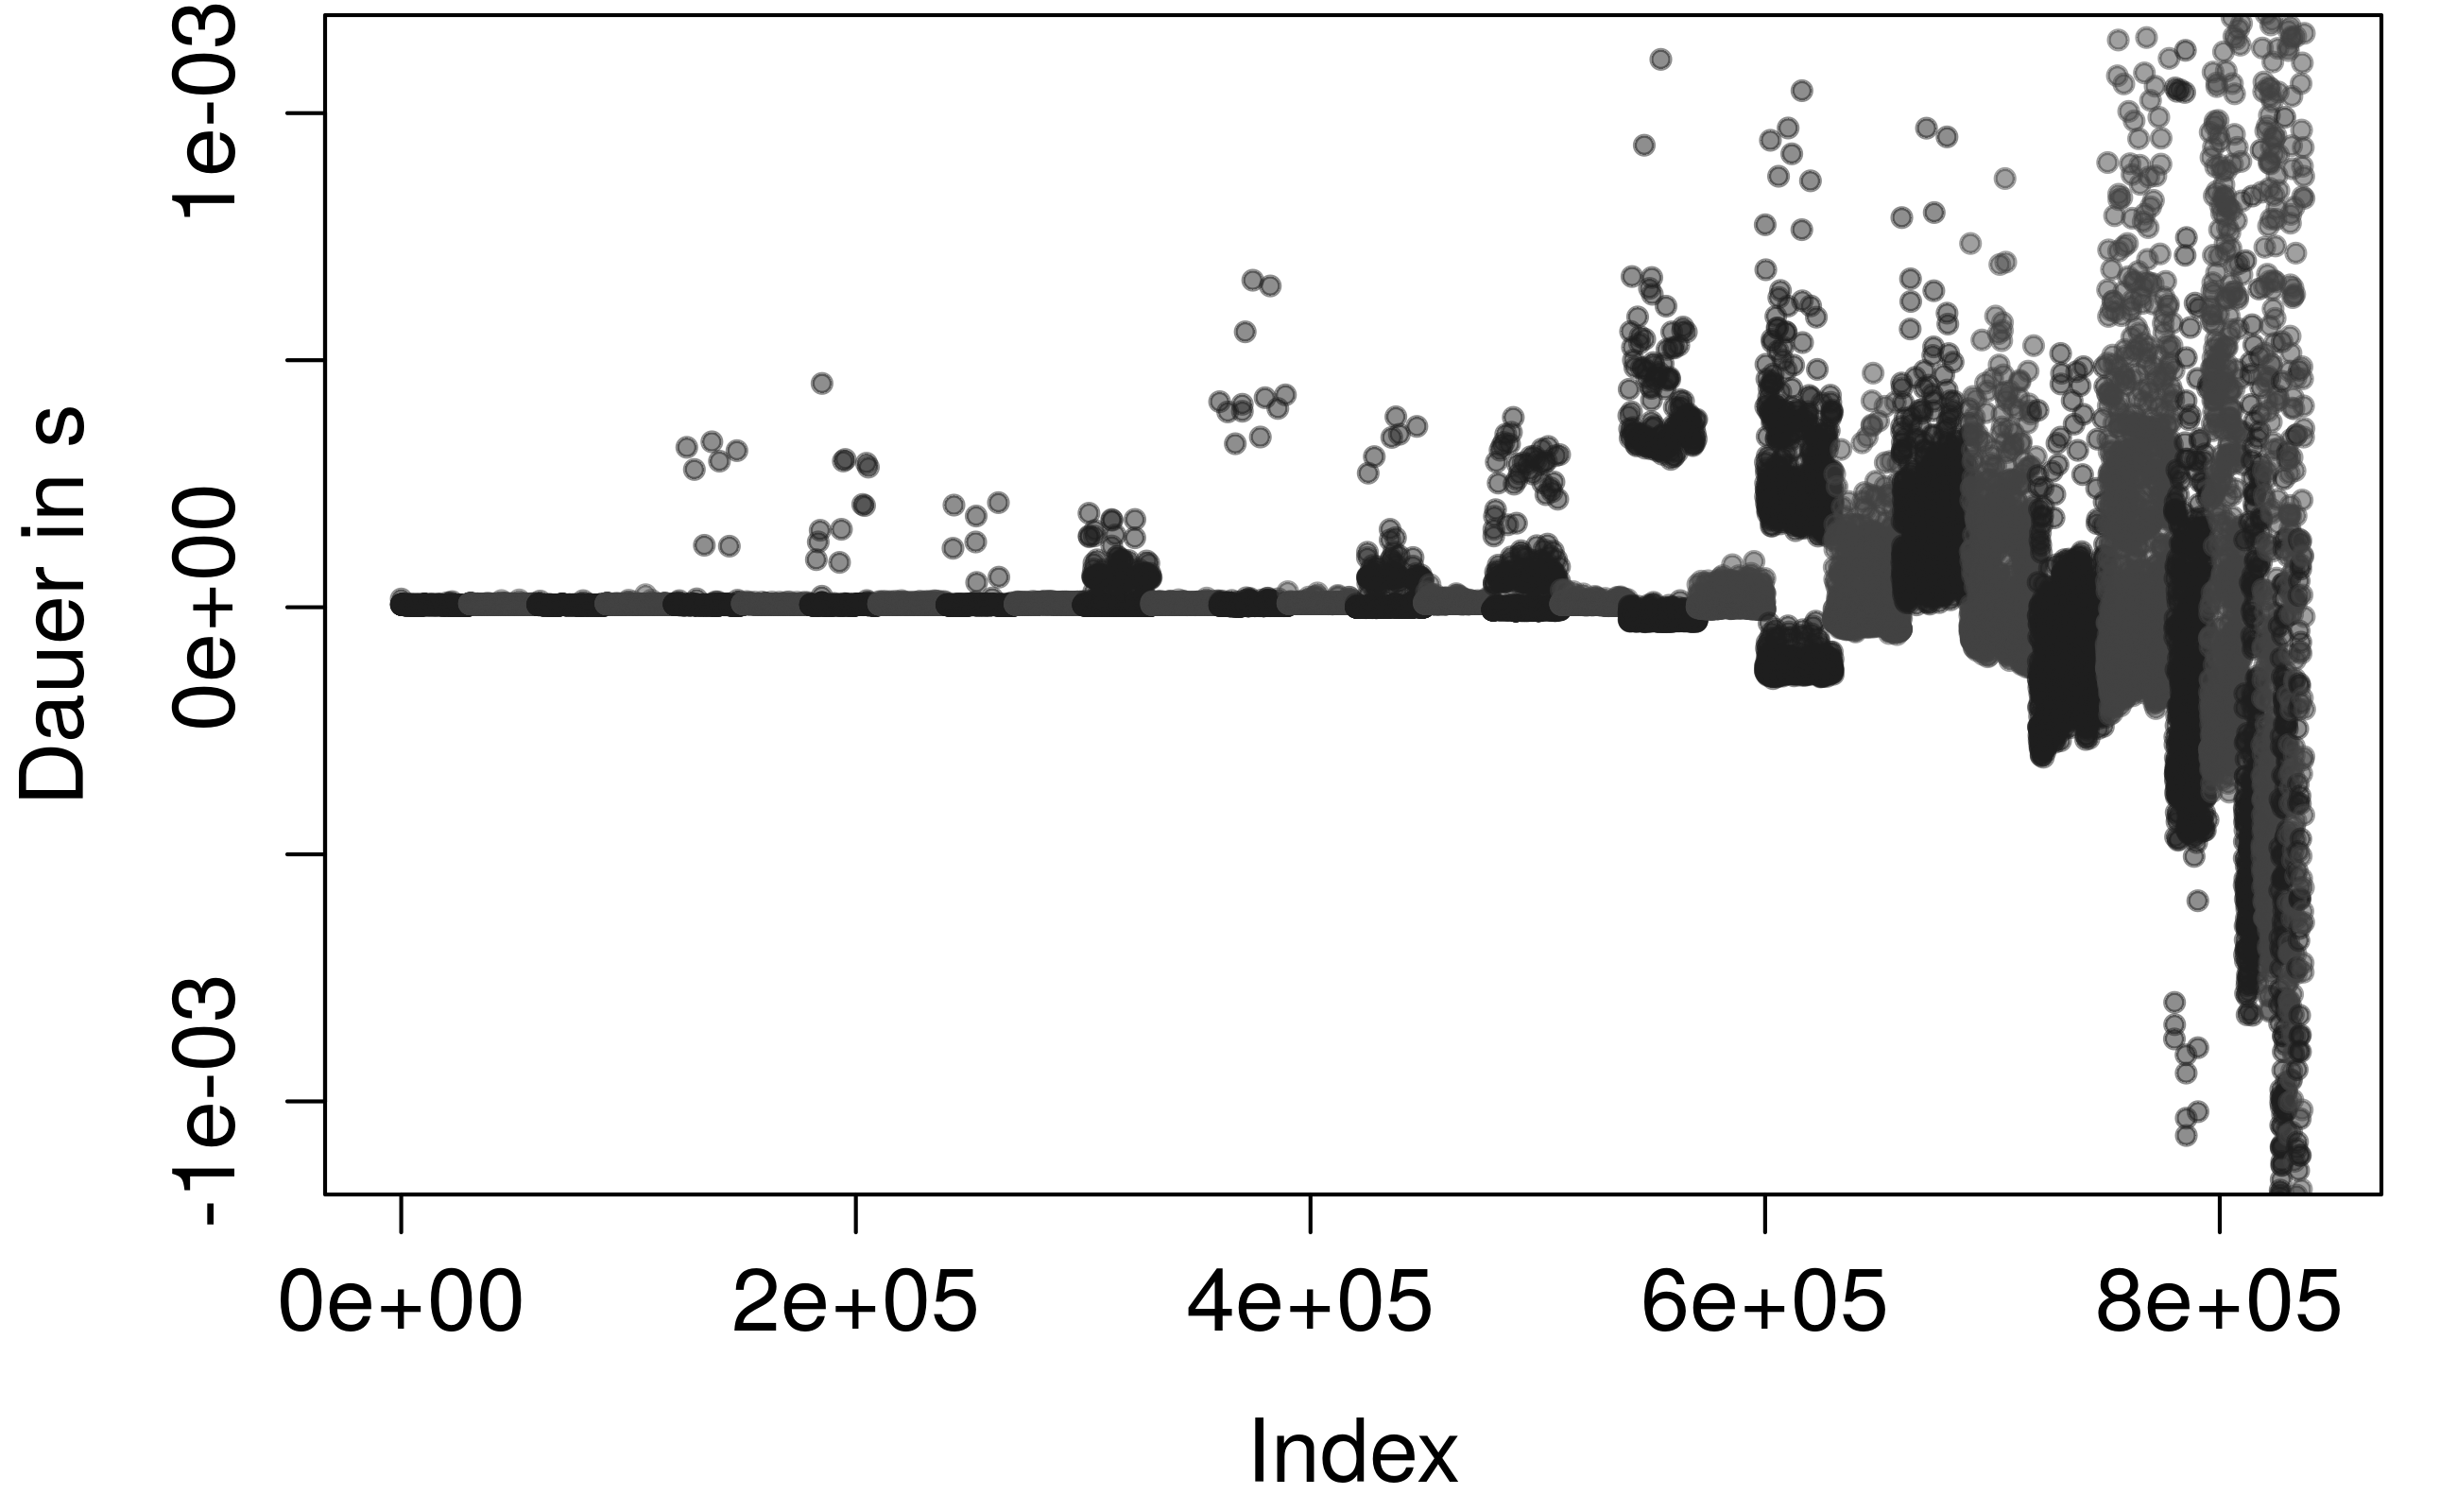
\includegraphics[width=.43\textwidth]{Bilder/Plots/error_class/exploration/linreg_error_seq_all.png}
	}
	\subfloat[Farblich markierte Fehlerklassen, begrenzte Y-Achse]{
		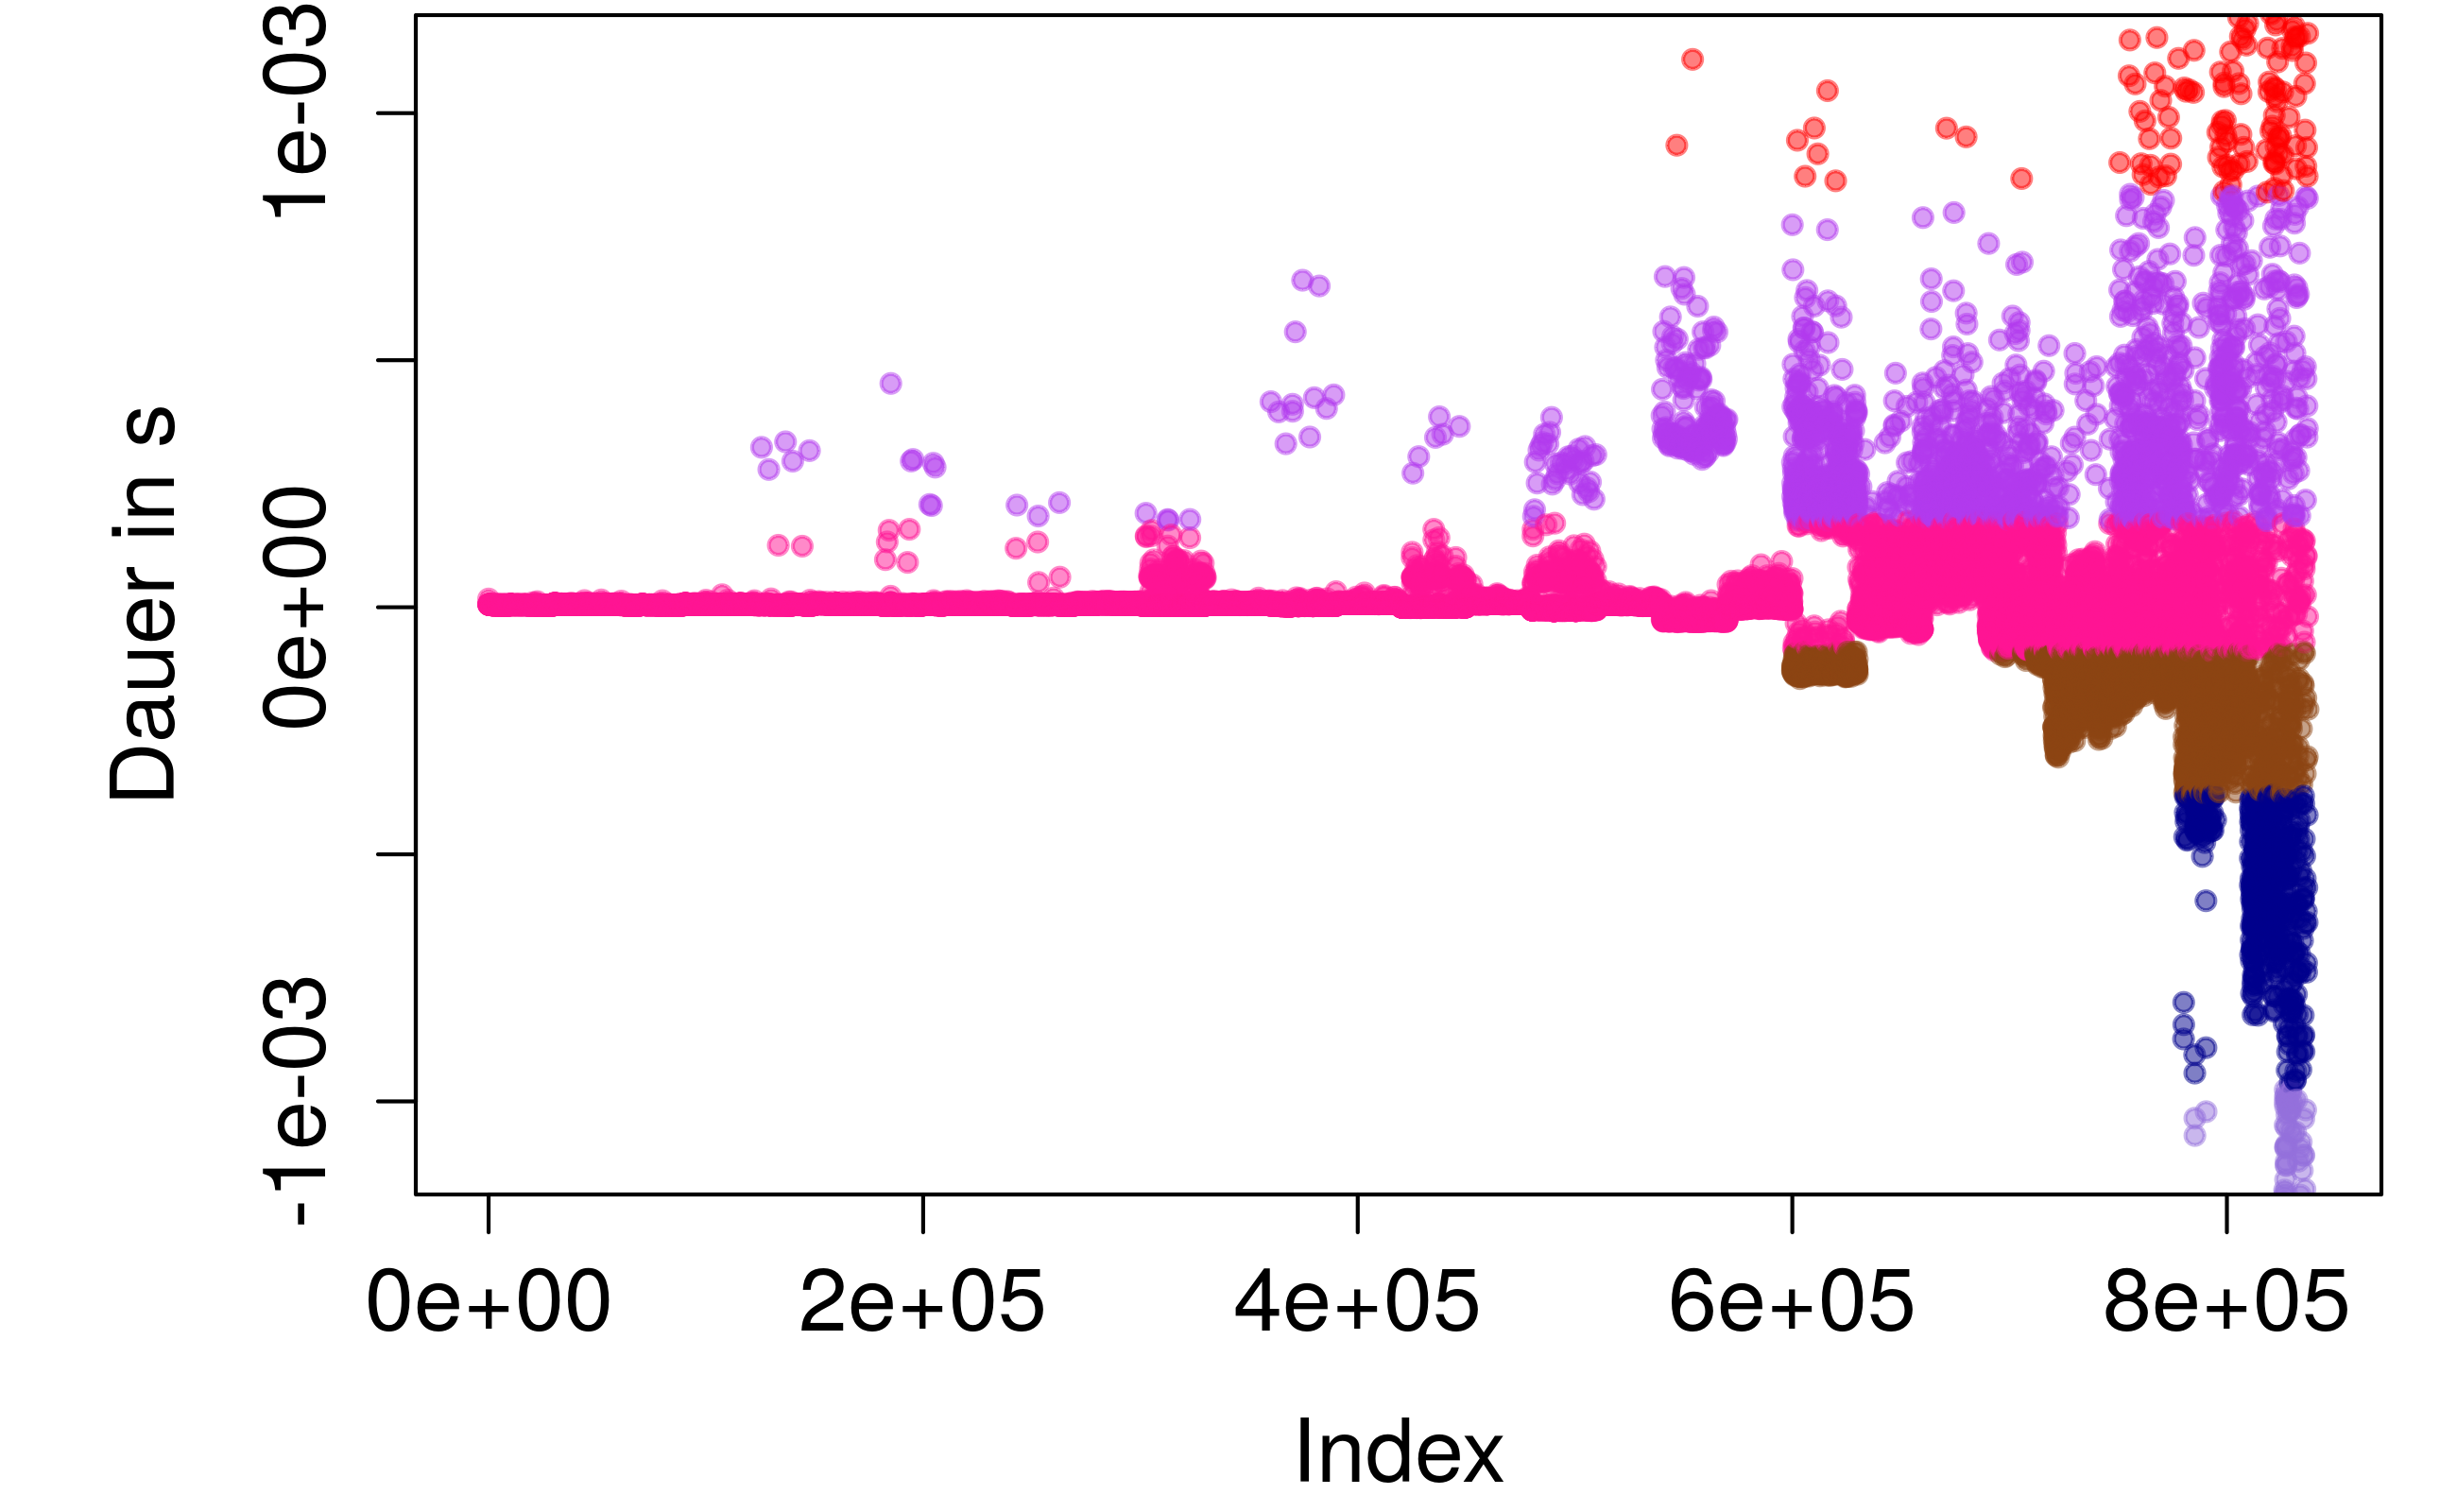
\includegraphics[width=.43\textwidth]{Bilder/Plots/error_class/exploration/linreg_error_clustering_seq_all.png}
	}\\
	\subfloat[Sortiert nach Modellabweichung, alle Punkte gezeichnet]{
		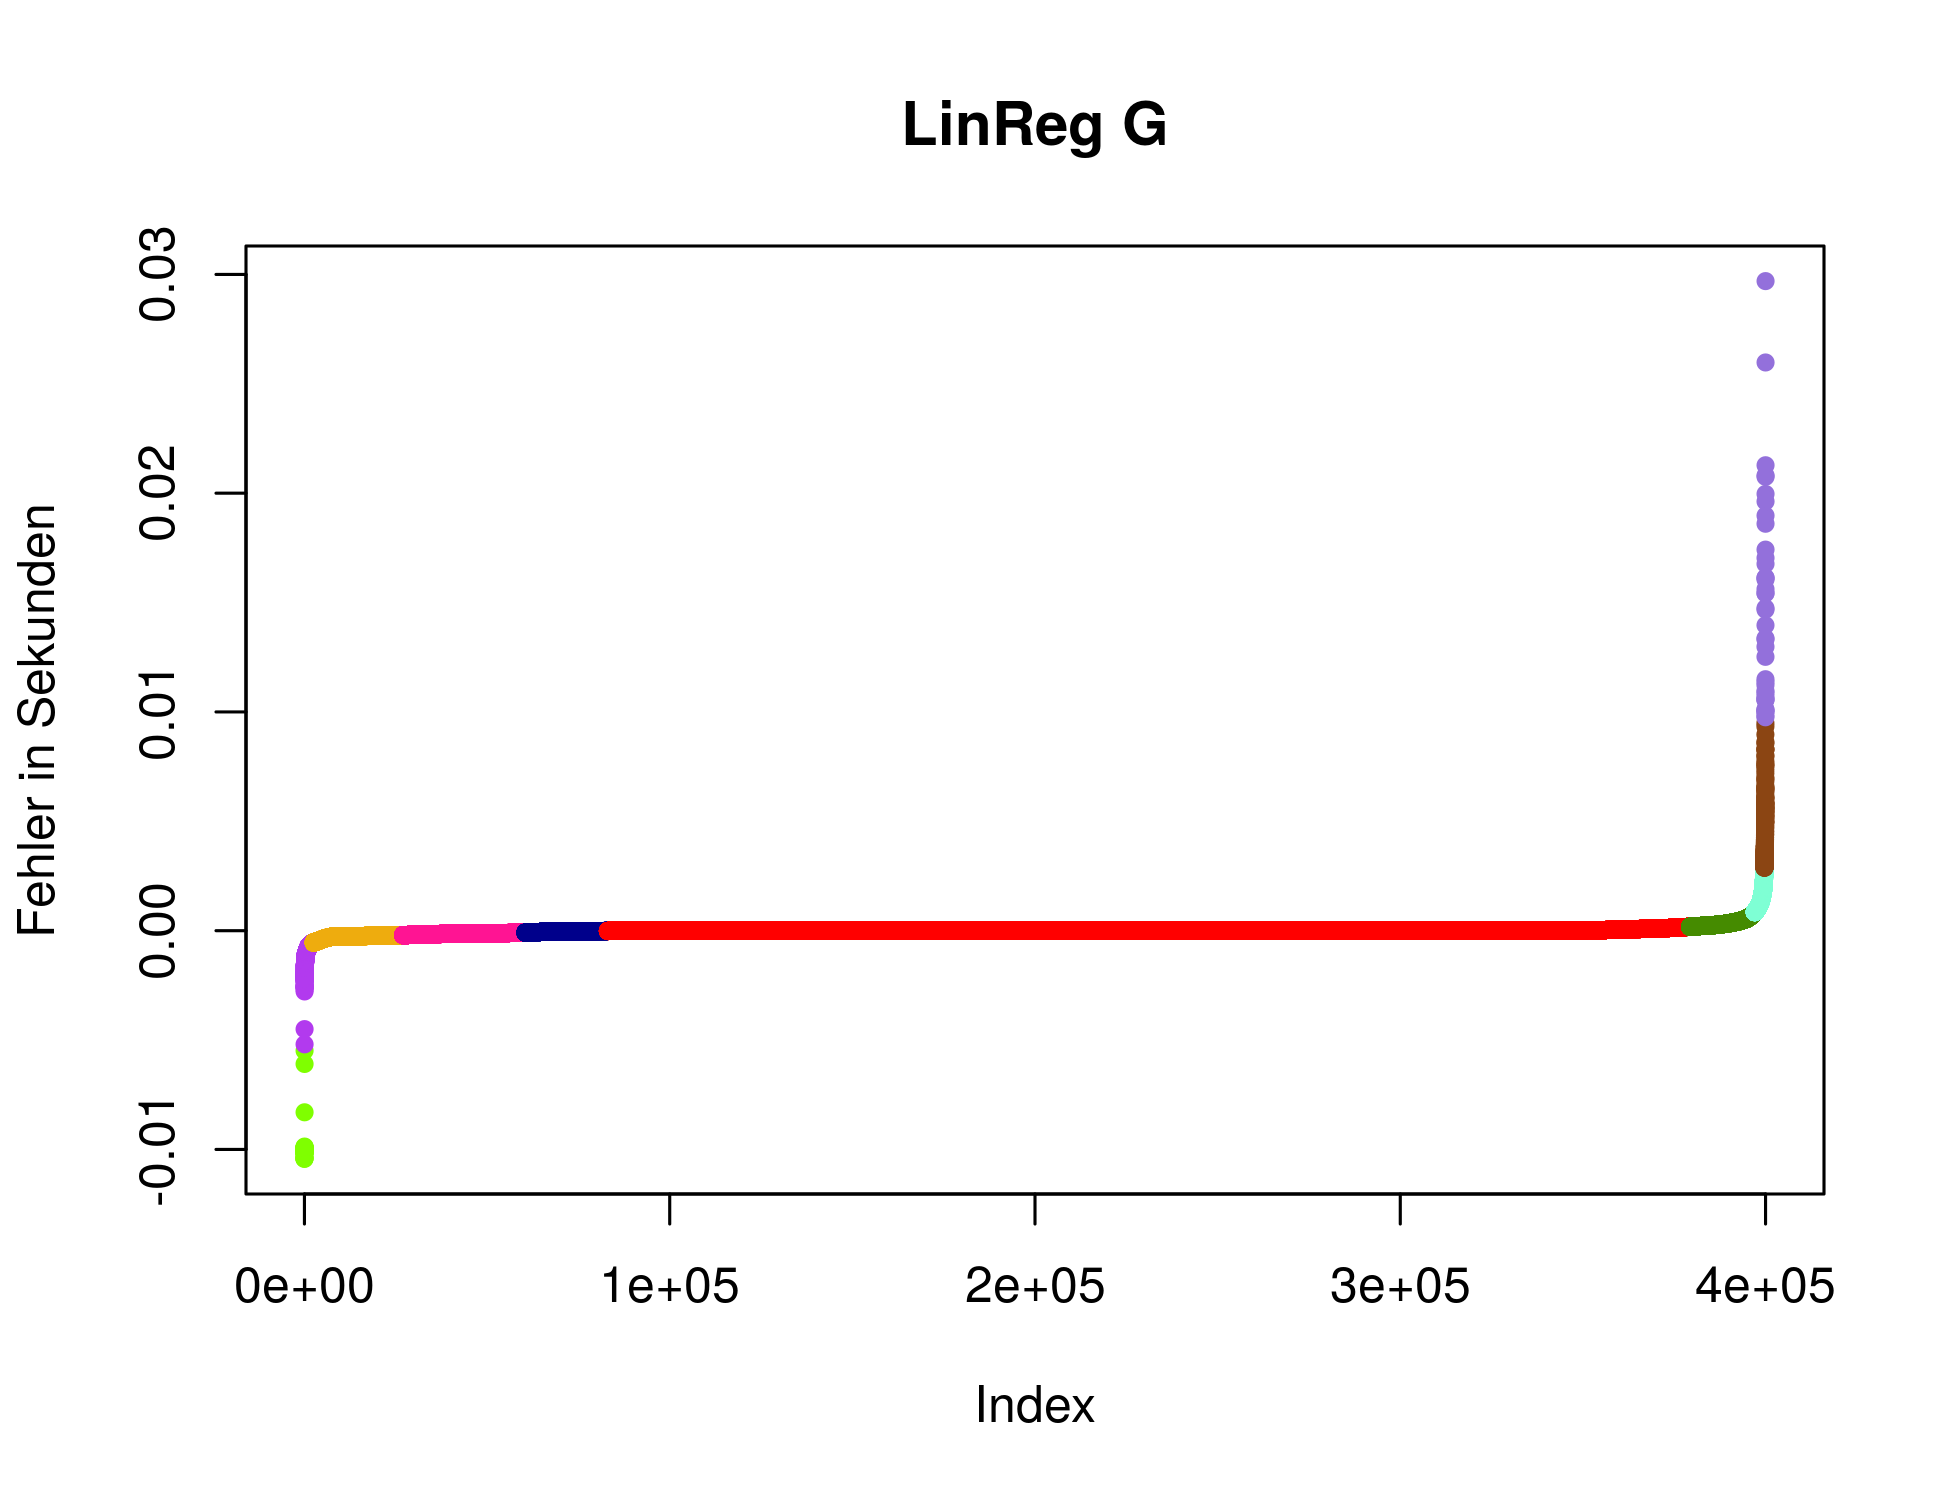
\includegraphics[width=.43\textwidth]{Bilder/Plots/error_class/exploration/linreg_error_sorted_clustering_seq.png}
	}
	\subfloat[Dichte der drei Klassen um den Nullpunkt]{
		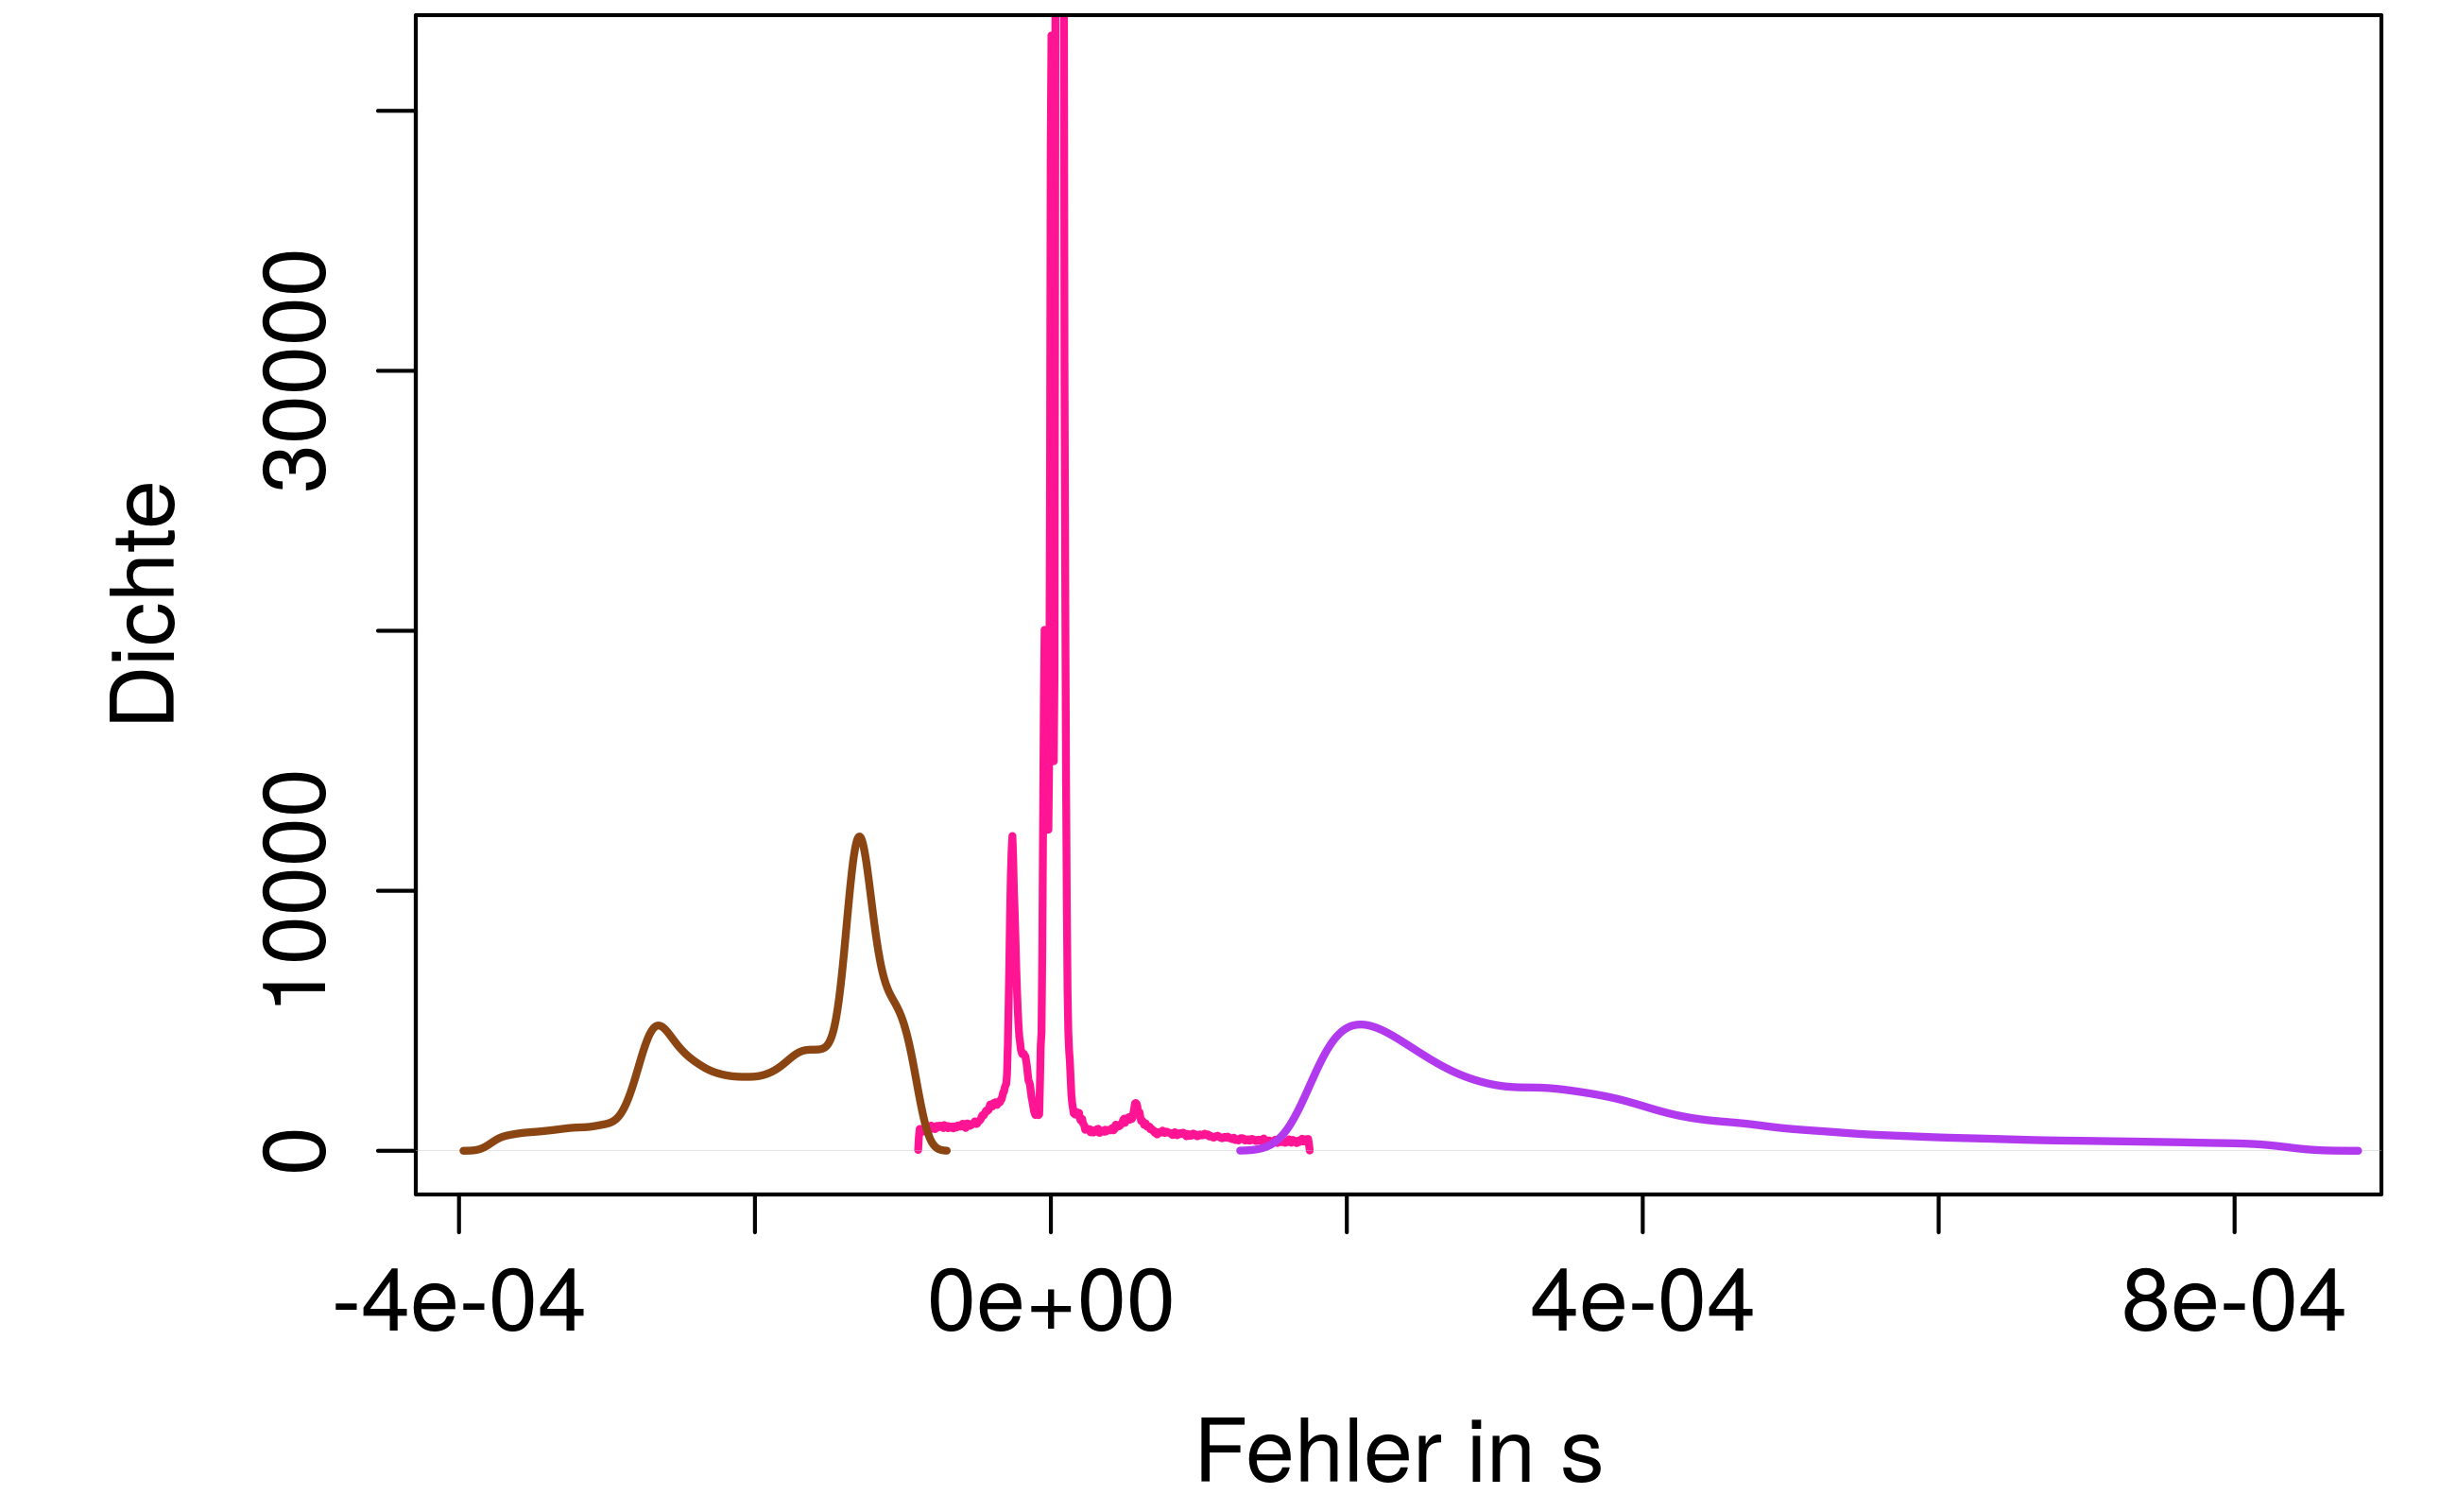
\includegraphics[width=.43\textwidth]{Bilder/Plots/error_class/exploration/density_of_fk_seq.png}
	}
	\caption{Verwendung des K-Means Algorithmus zur Bestimmung der Fehlerklassen auf den Messungen mit sequentiellen Dateizugriff aus der Vorhersage von \glqq LinReg G\grqq}
	\label{fig:error_class_clustering_seq}
\end{figure} 

In den Graphen jeweils rechts neben den beschriebenen ist durch farbliche Markierung die Zugehörigkeit der Messpunkte zu ihren Fehler-Klassen erkennbar.
Die Unterscheidung in verschiedene Klassen findet in horizontalen Linien statt. Eine Klasse deckt einen bestimmten Bereich der Fehlerwerte ab.
Die Fehlerklassen zu den sequentiellen Messungen differenzieren nur bei den höheren Zugriffsgrößen, bei den zufälligen Zugriffen ist dies nicht der Fall
Bei der Betrachtung der Graphen in denen nach Fehler sortiert wurde ( \ref{fig:error_class_clustering_seq}c, sowie \ref{fig:error_class_clustering_rnd}c ) können die Anzahlen der jeweils zugeordneten Punkte zu den Klassen gut quantifiziert werden.
In beiden Fällen enthält eine Klasse den Großteil der Punkte. Die Klassen, dessen abgedeckte Bereiche nur leicht abweichen, enthalten noch einen kleineren Anteil der Messdaten.
Die Ausreißer in beide Richtungen machen quantitativ fast nichts aus, werden allerdings durch mehrere Klassen abgedeckt. So werden die obersten 5\% der Modellabweichungen vom sequentiellen Datensatz in 5 Klassen aufgeteilt.

Die beiden Abbildungen \ref{fig:error_class_clustering_seq} d) und \ref{fig:error_class_clustering_rnd}d zeigen die Dichteverteilung der Fehlerklasse, die den kleinsten Fehler abdeckt, sowie der nächst kleineren und größeren Fehlerklasse.
Idealerweise sollte die Dichte einer Fehlerklasse nur eine Spitze enthalten. Die Klasse repräsentiert dann einen Fehlerbetrag, der dann einem E/A-Pfad entspricht.
Auf den sequentiellen Daten weisen die Dichten der Fehlerklasse links vom Nullpunkt, sowie die um den Nullpunkt, zwei klar voneinander unterscheidbare Spitzen auf.
Während die Verteilung der Dichte rechts vom Nullpunkt auf den randomisierten Daten gar keine Spitze hat. Diese Klasse stellt daher keinen E/A-Pfad da.
Diese Beobachtungen könnten darauf hinweisen, dass auf den Messungen mit sequentiellen Zugriff eigentlich eine größere Anzahl Cluster-Gruppen benötigt worden wäre, um alle E/A-Pfade zu repräsentieren, während bei den Messungen mit zufälligen Dateizugriffen weniger genutzt werden müssten. 

Das Modell \textit{LinReg G} scheint generell schon recht gut zu sein, da die Fehler sich für die Klassen mit dem kleinsten durchschnittlichen Fehler sammeln.
Es gibt allerdings einige Datenpunkte, die das Modell sehr schlecht vorhersagen konnte. Die Annahme ist nun, dass die Messergebnisse mit stark abweichenden Residuen im Allgemeinen unterschiedlich vom System verarbeitet wurden. 
Sodass die Fehlerklassen die unterschiedlichen E/A-Wege im System repräsentieren. 
Wobei immer beachtet werden muss, dass die Vorhersage von Messungen mit höheren Zugriffsgrößen auch zu größeren Abweichungen führt.
Ein Modell, dass eine Modellierung mit dem zusätzlichen Wissen dieser Klassenzuordnungen vornimmt, sollte die Ausreißer, die \textit{LinReg G} schlecht bestimmt hat, wesentlich besser vorhersagen können.
Für die Vorhersage der vielen Datenpunkte, die sich in der jeweils größten Klasse befinden, hat ein Modell mit Fehlerklasseninformationen jedoch keine weiteren Vorteile. 

\begin{figure}
	\centering
	\subfloat[Sortiert nach Zugriffsgröße, in $\text{}$ dunkelgrau lesende und in hellgrau schreibende Zugriffe, begrenzte Y-Achse]{
		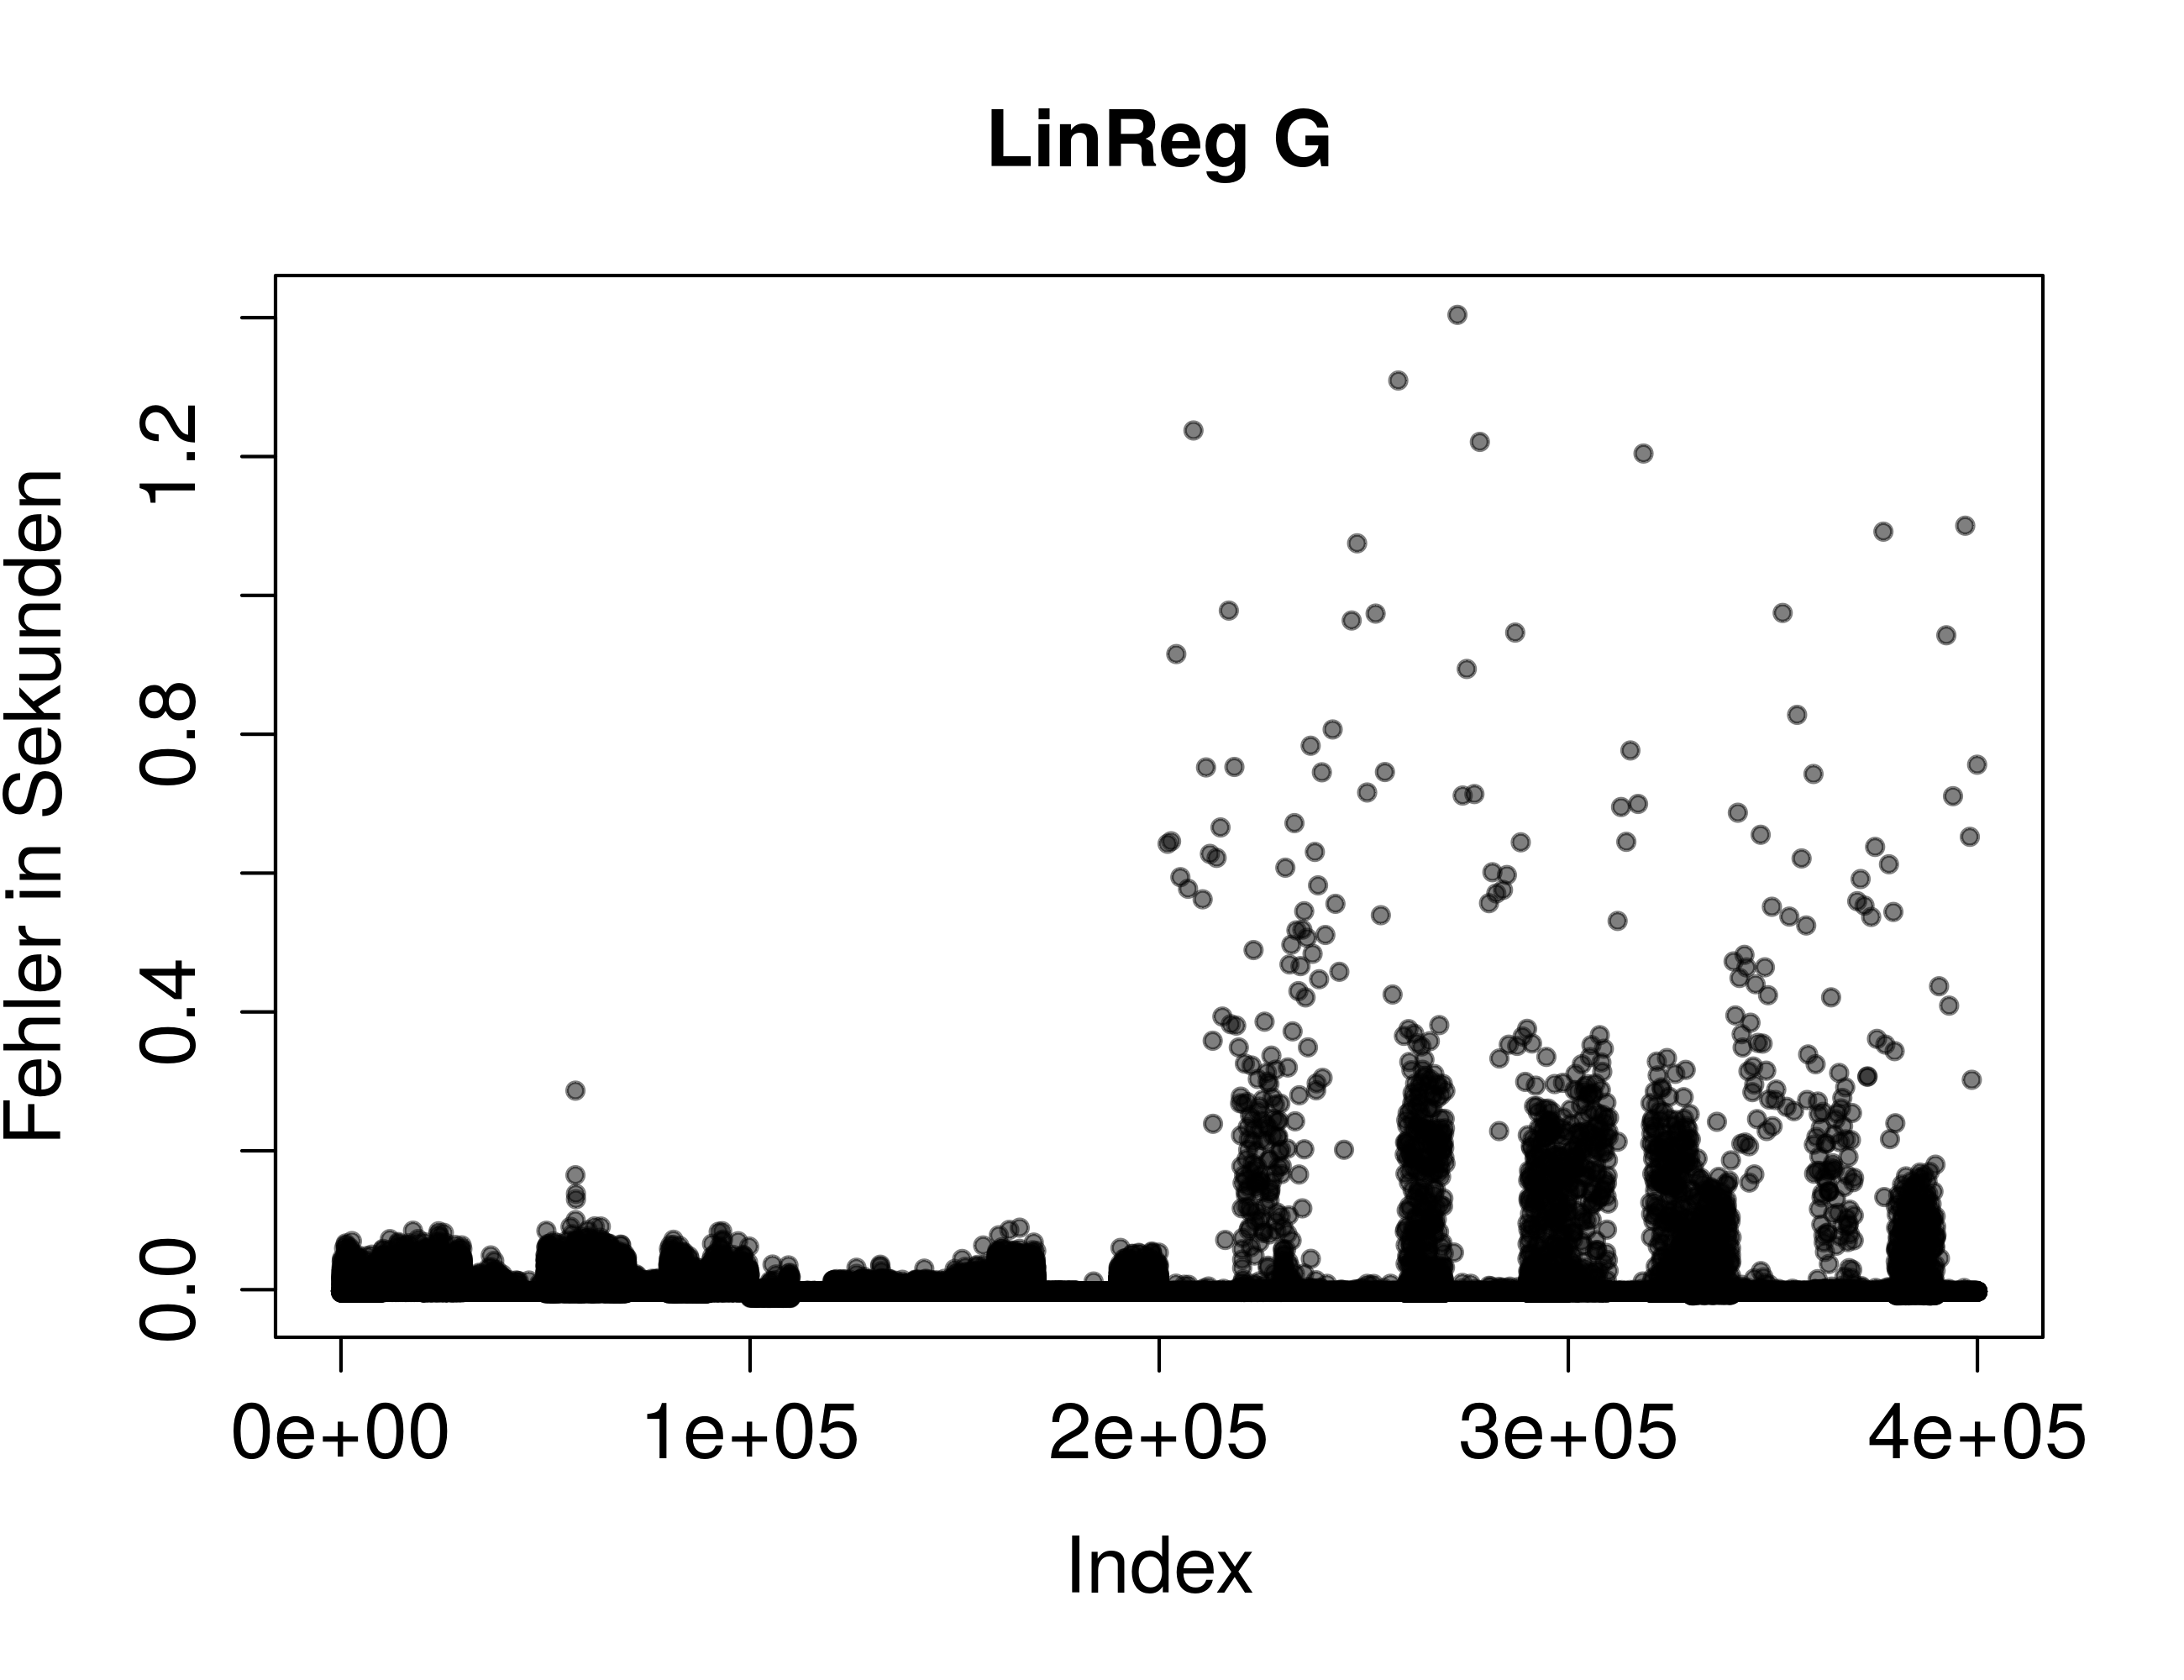
\includegraphics[width=.43\textwidth]{Bilder/Plots/error_class/exploration/linreg_error_rnd_all.png}
	}
	\subfloat[Farblich markierte Fehlerklassen, begrenzte Y-Achse]{
		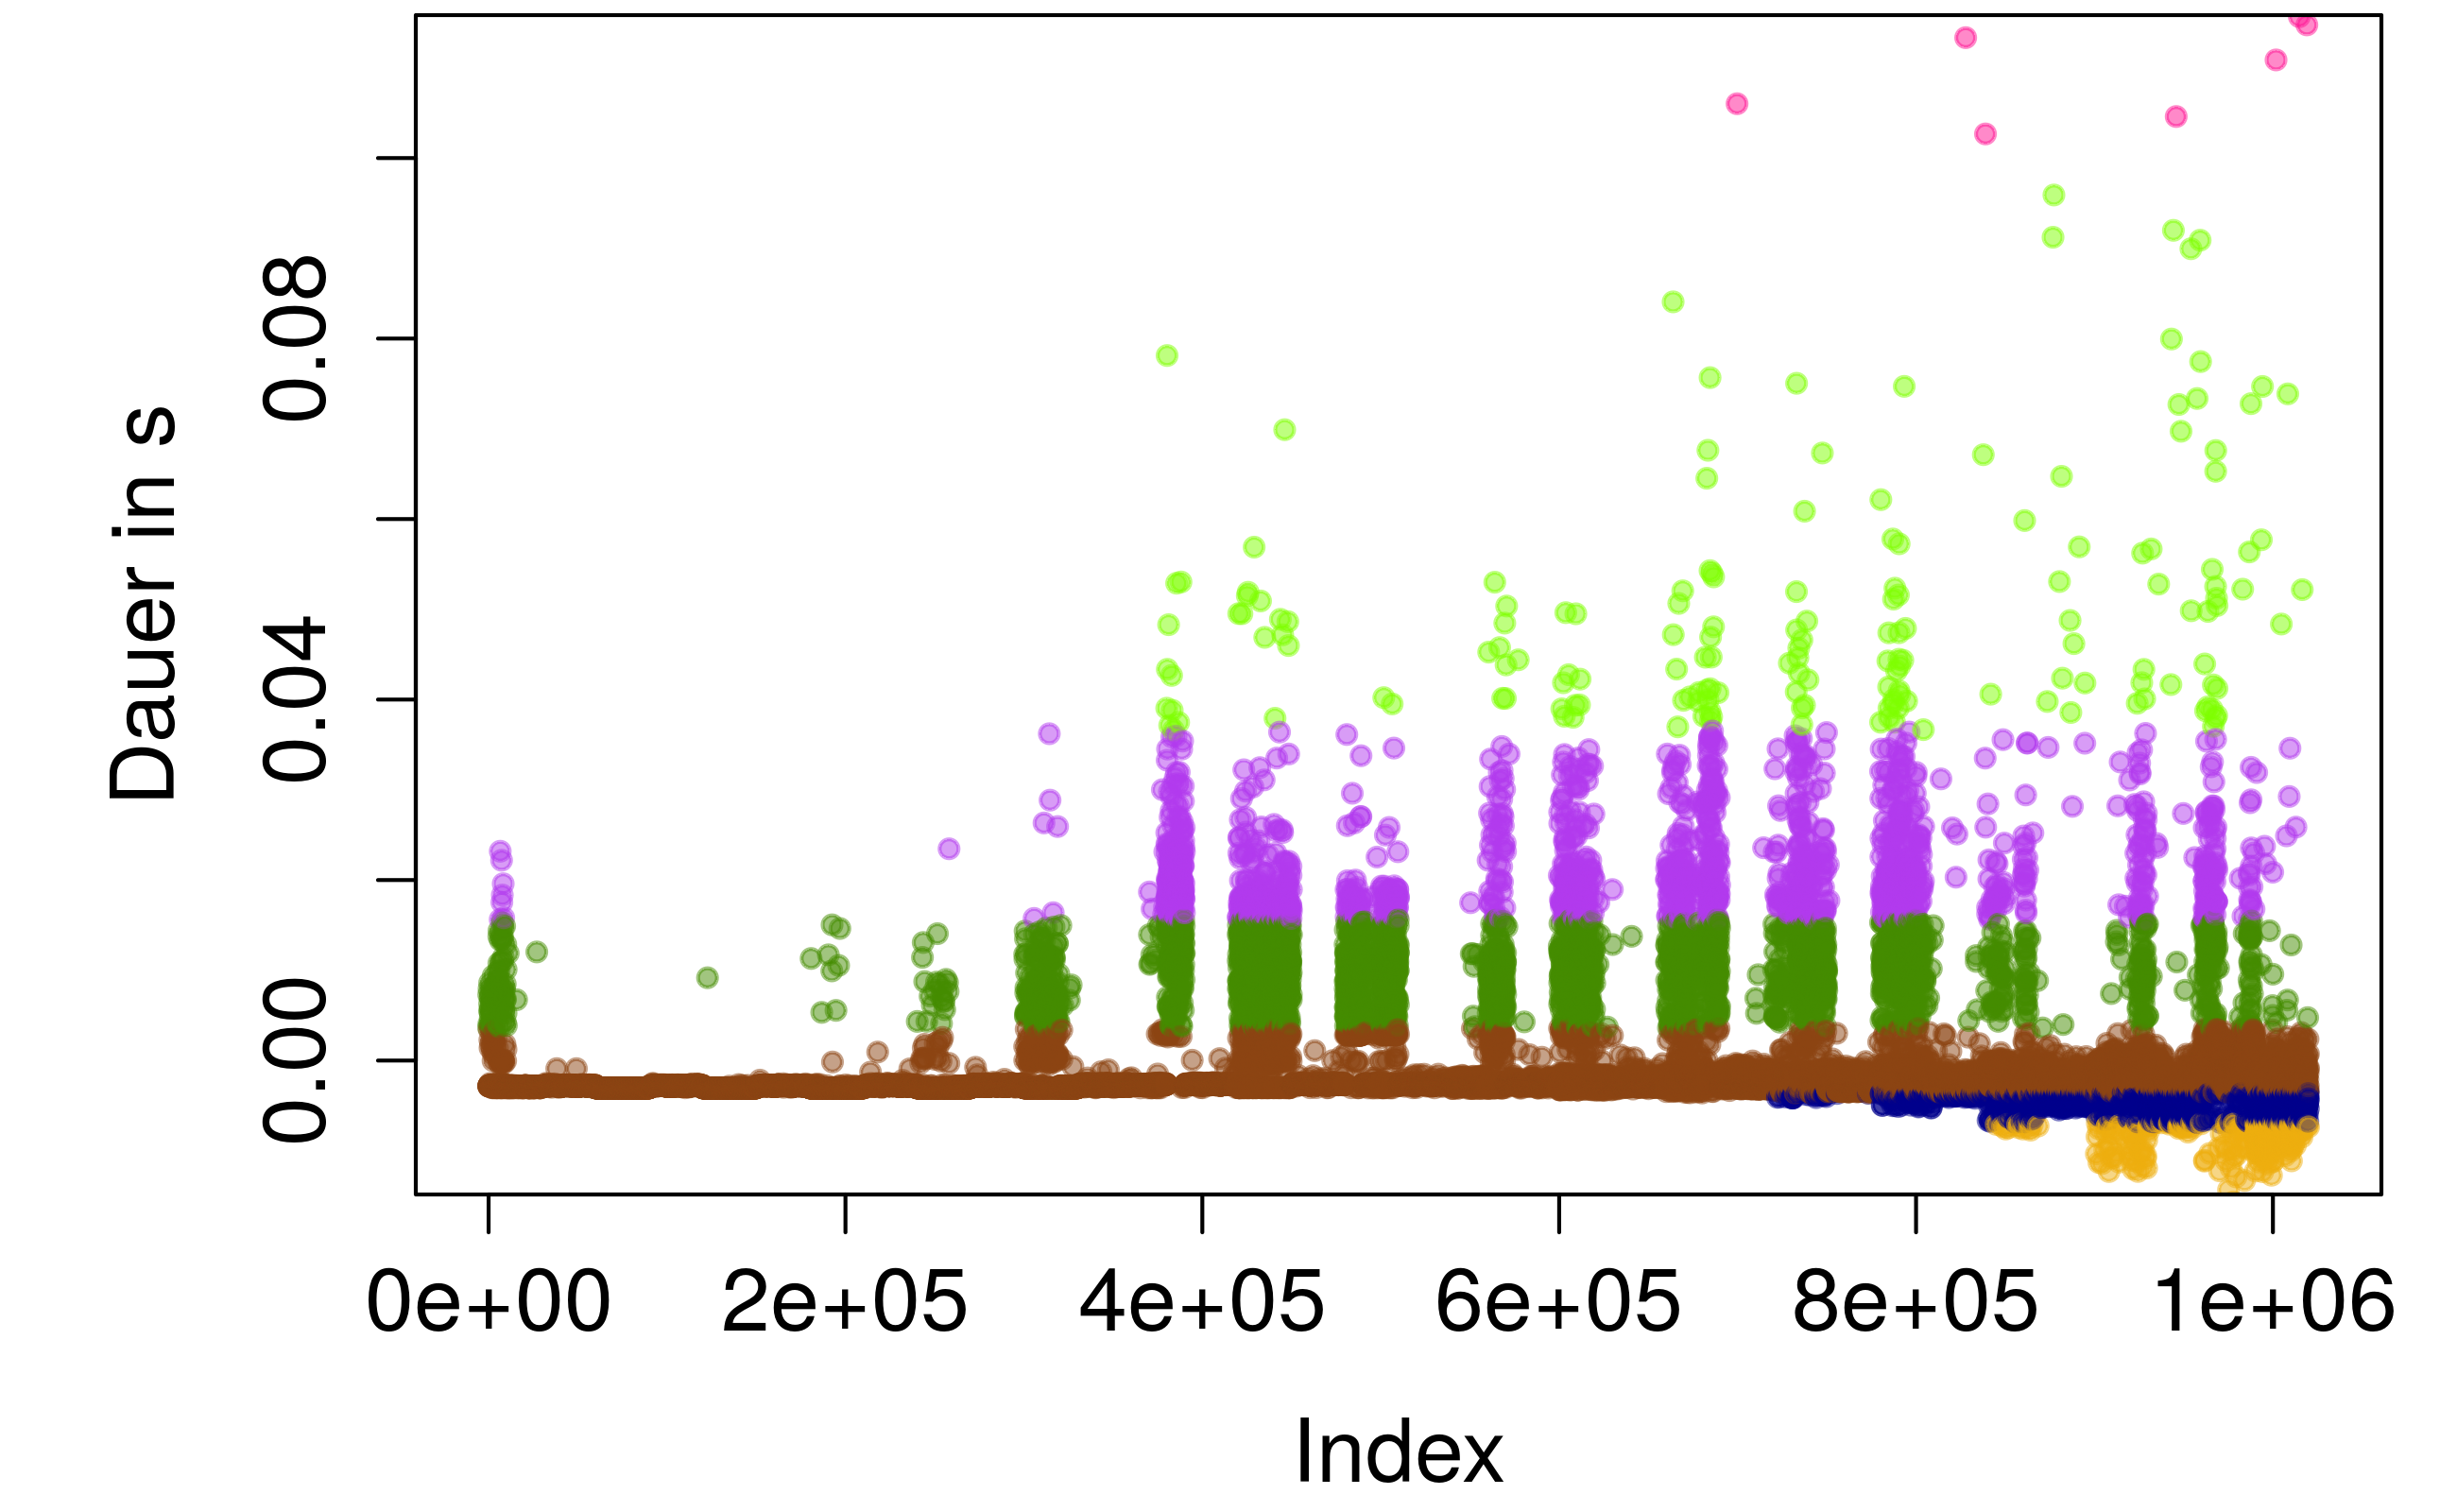
\includegraphics[width=.43\textwidth]{Bilder/Plots/error_class/exploration/linreg_error_clustering_rnd_all.png}
	}\\
	\subfloat[Sortiert nach Modellabweichung, alle Punkte gezeichnet]{
		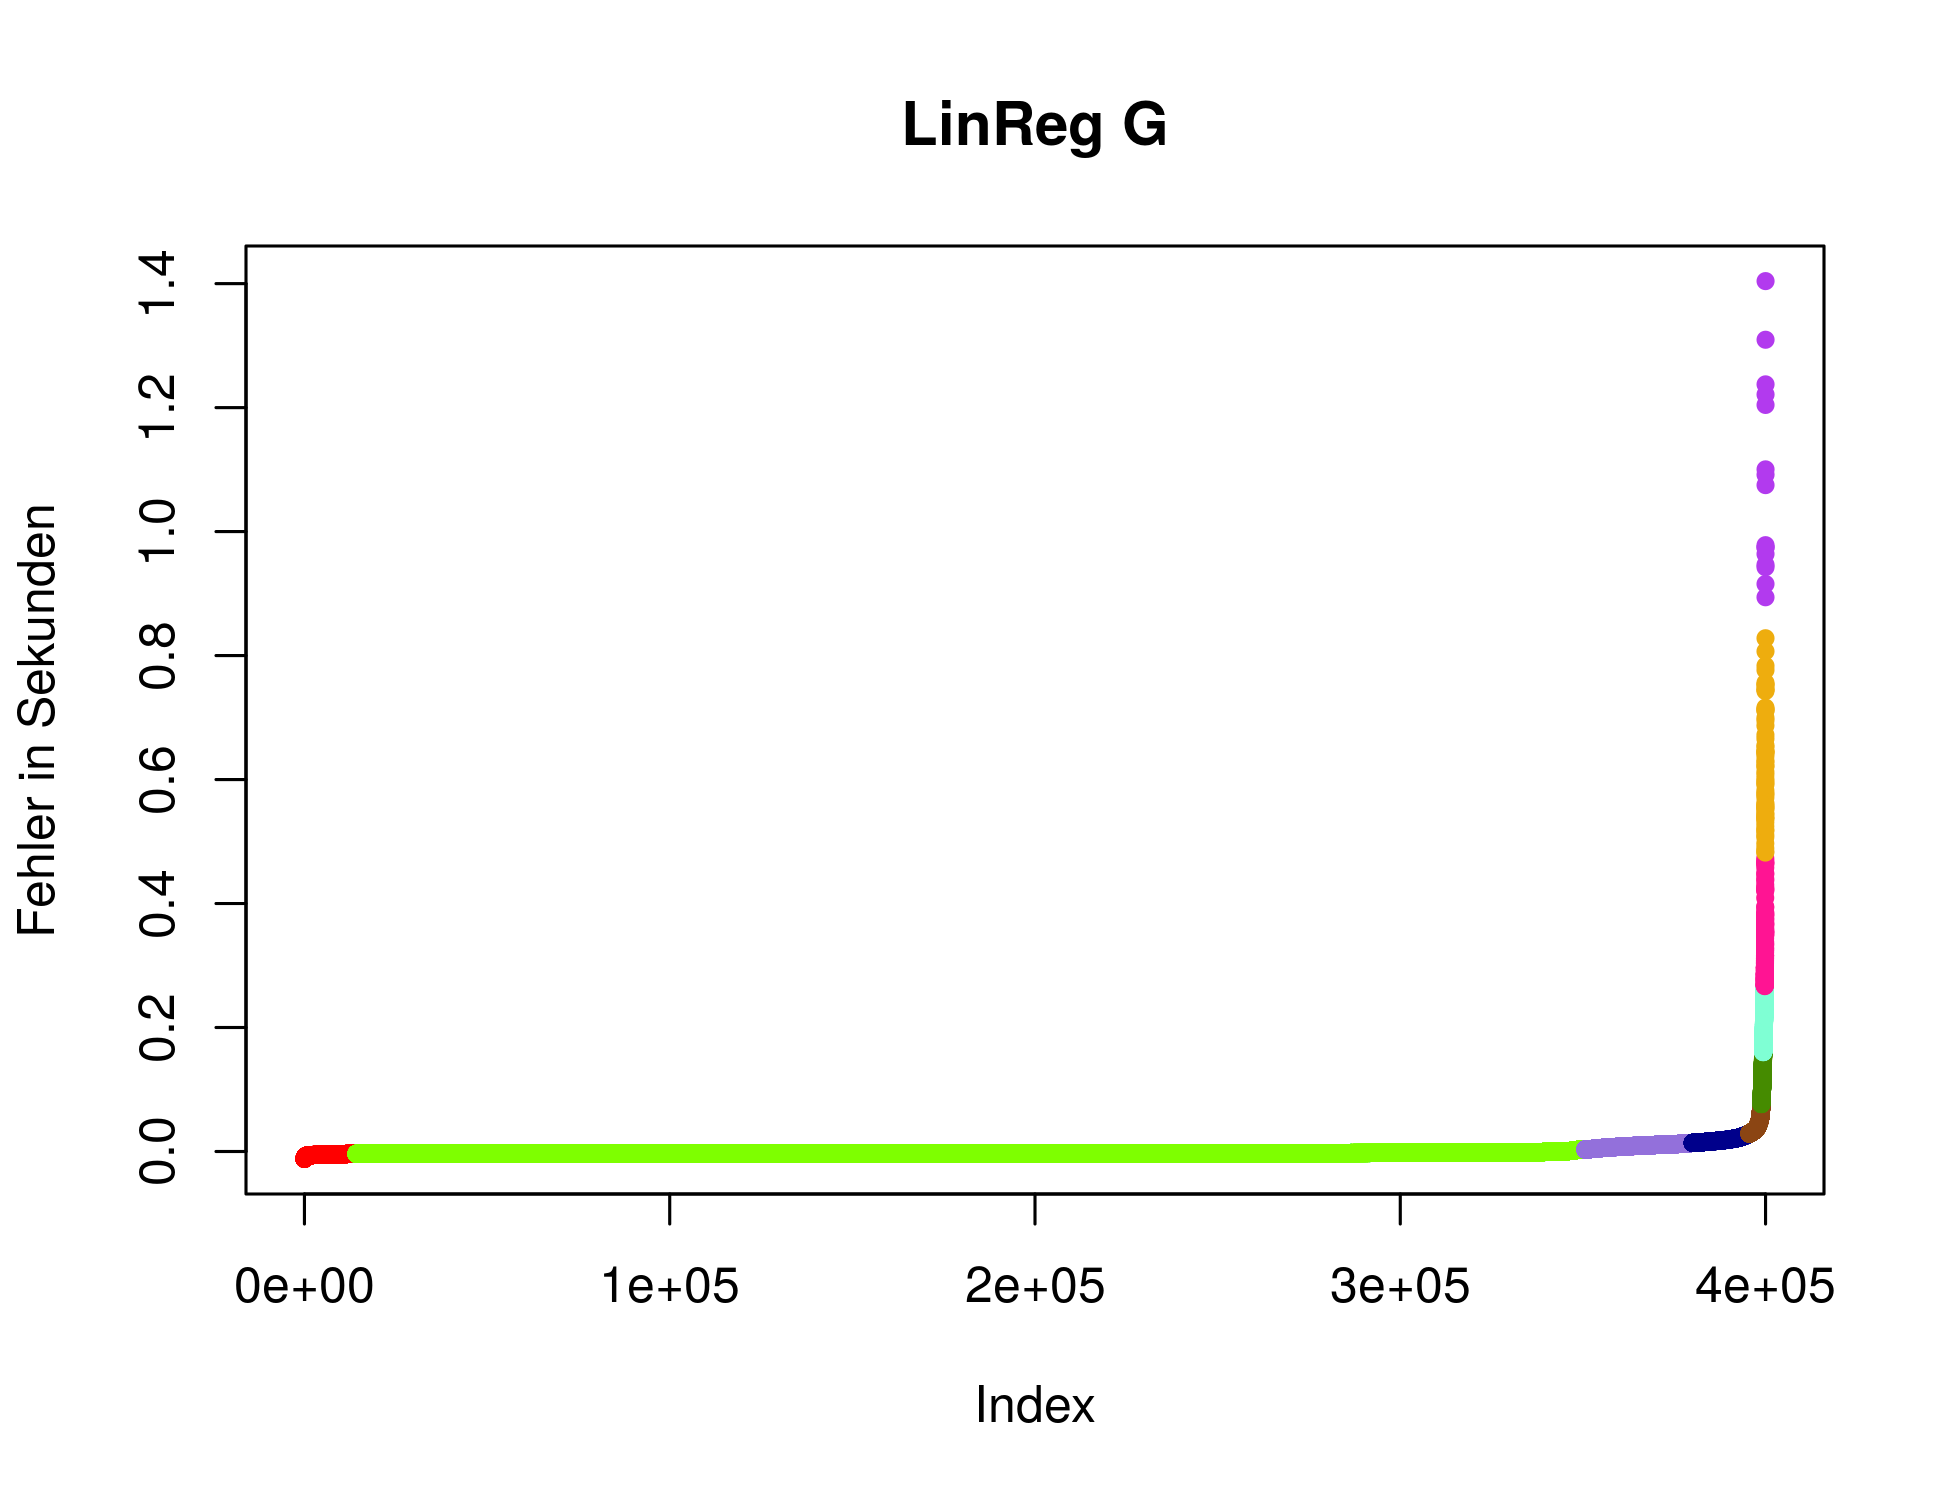
\includegraphics[width=.43\textwidth]{Bilder/Plots/error_class/exploration/linreg_error_sorted_clustering_rnd.png}
	}
	\subfloat[Dichte der drei Klassen um den Nullpunkt]{
		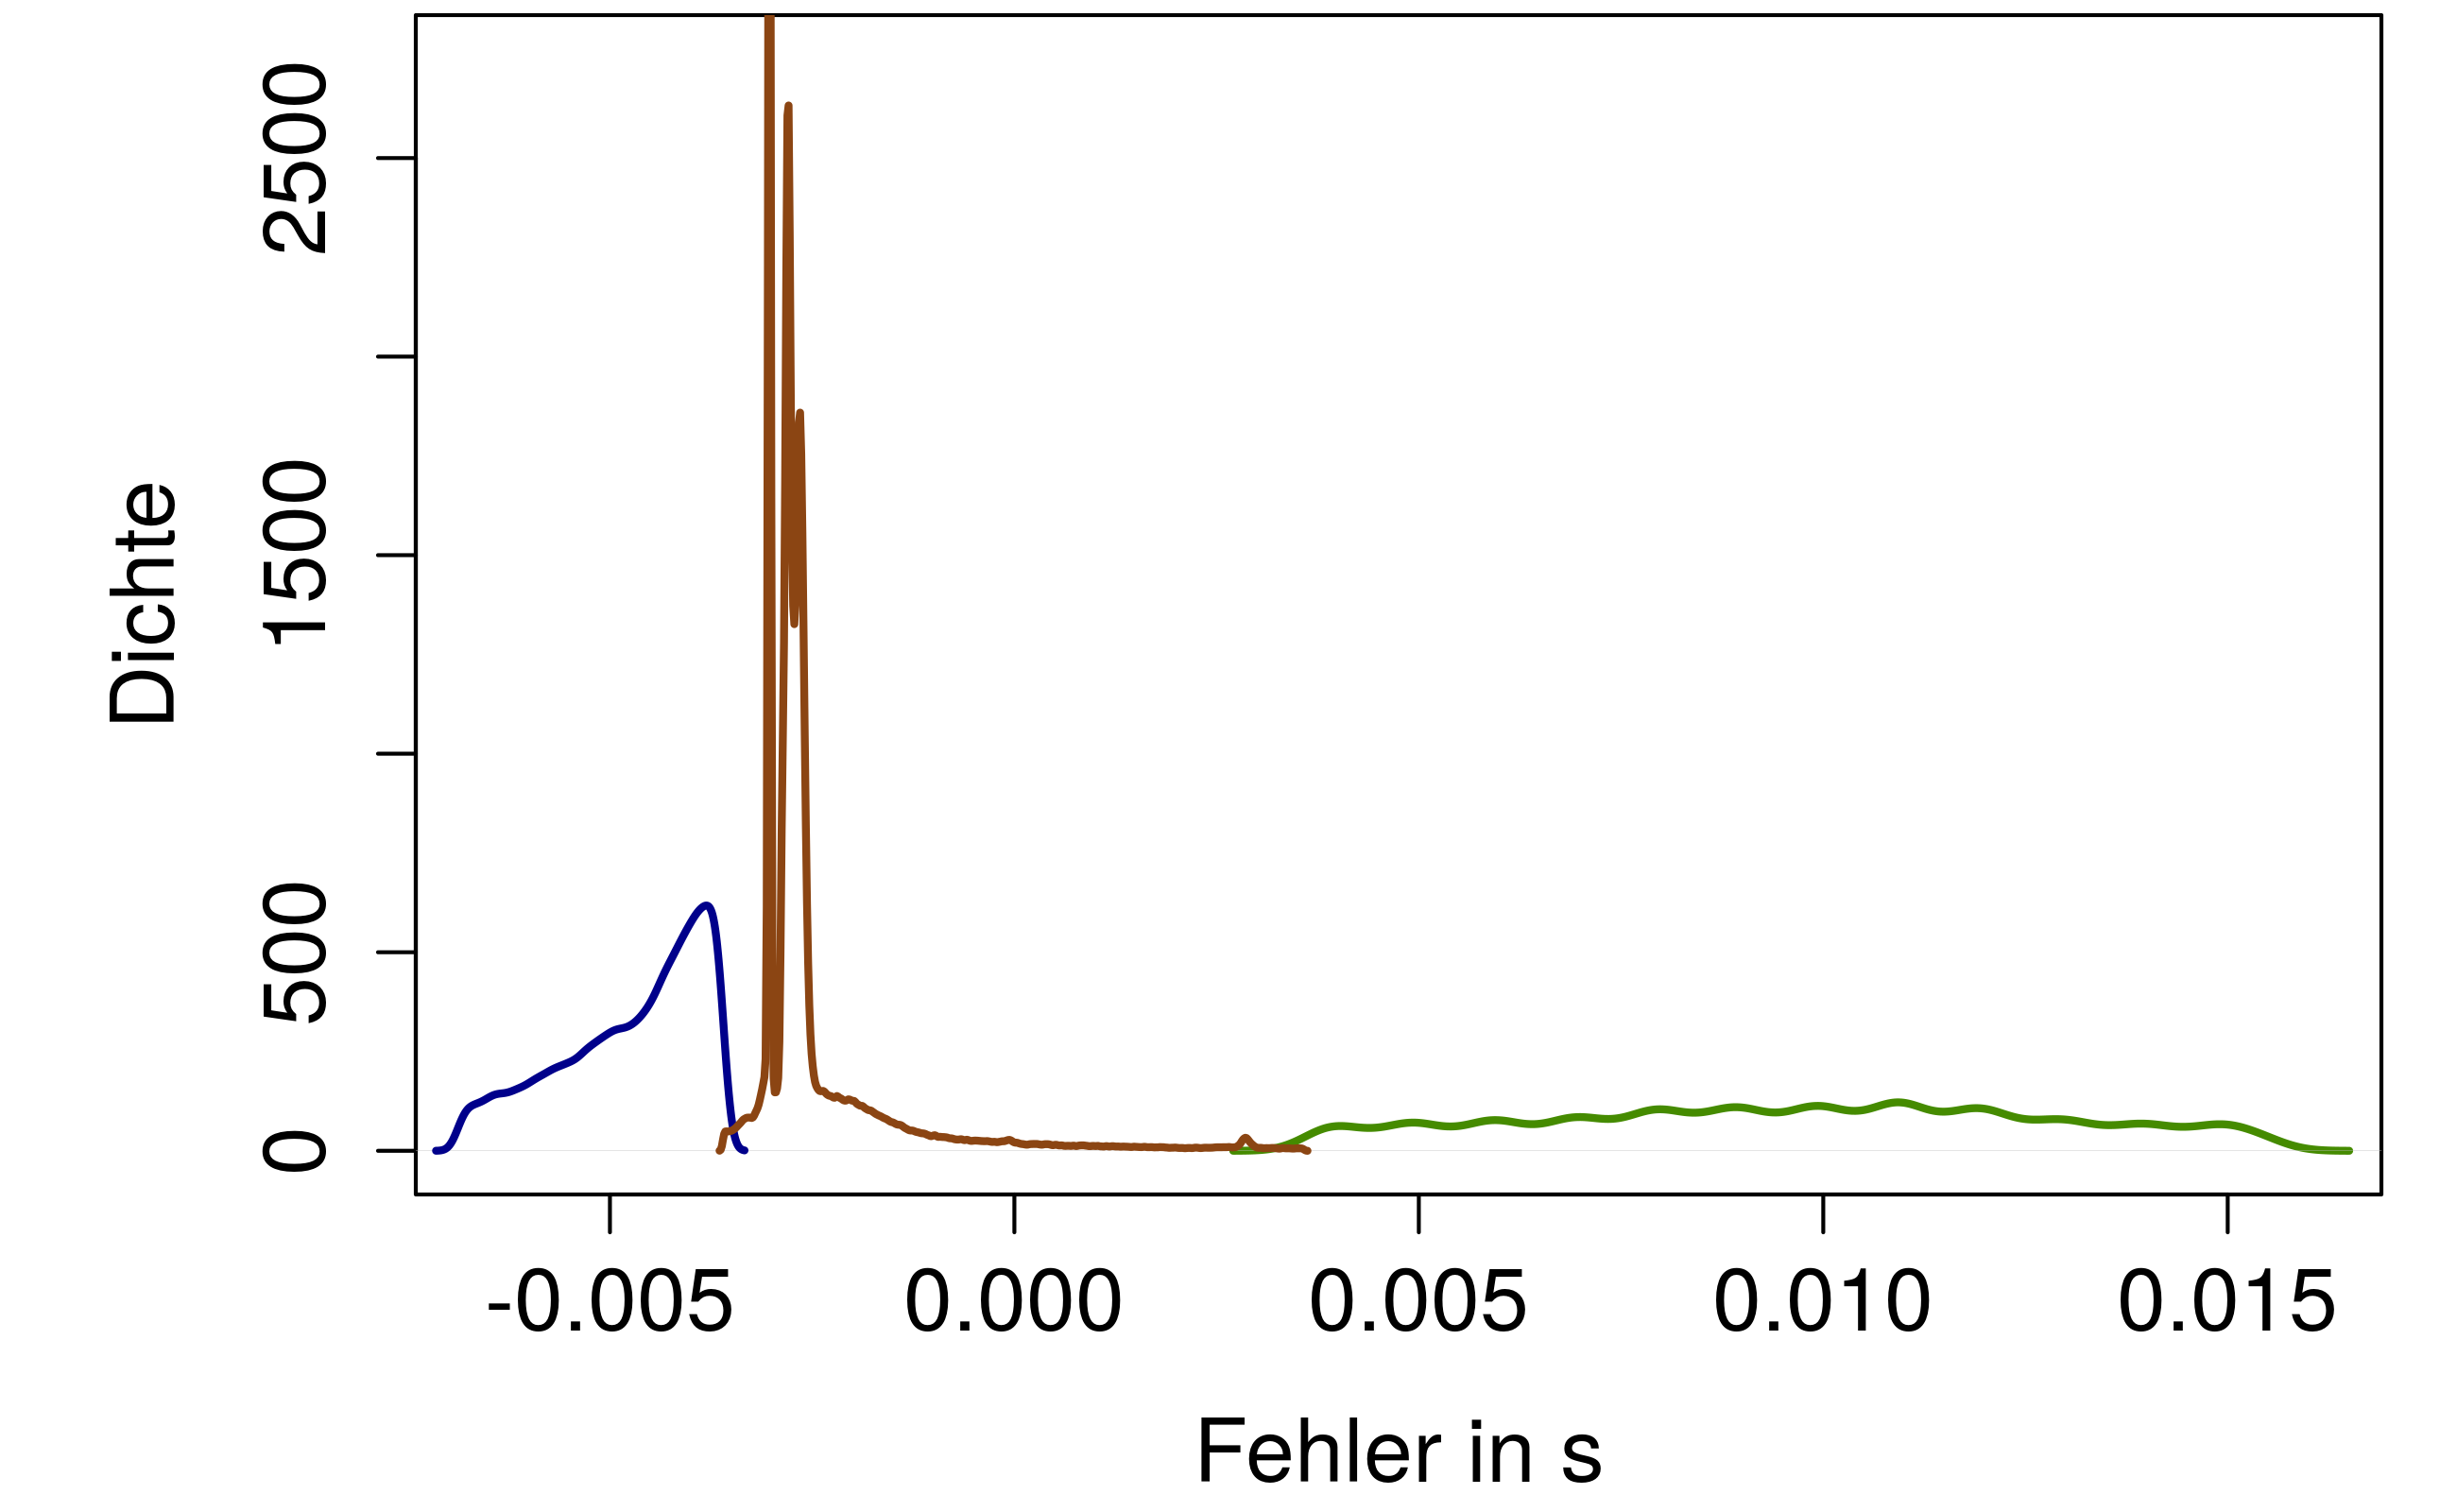
\includegraphics[width=.43\textwidth]{Bilder/Plots/error_class/exploration/density_of_fk_rnd.png}
	}
	\caption{Verwendung des K-Means Algorithmus zur Bestimmung der Fehlerklassen auf den Messungen mit zufälligem Dateizugriff aus der Vorhersage von \glqq LinReg G\grqq}
	\label{fig:error_class_clustering_rnd}
\end{figure} 

Anhand einer weiteren Betrachtung der Fehlerklassen sollen die Unterschiede zwischen den Klassen auf den beiden Datensätzen analysiert werden.
In Abbildung \ref{fig:error_classes_switched} sind die Punkte den Klassen aus dem jeweils anderen Datensatz zugeordnet worden. Die Neuzuordnung wurde ebenso durchgeführt, wie es der K-Means Algorithmus bei der Erstzuordnung gemacht hat.
Für alle Klassen wurde der mittlere Fehlerwert nach Zuordnung der Punkte auf dem ursprünglichen Datensatz berechnet und dann wurde jeder Datenpunkt im anderen Datensatz der Klasse mit dem Mittelwert zugeordnet, der am nächsten an seinem eigenen Fehlerwert liegt.

Für SEQ ist deutlich zu sehen, dass ein Großteil (tatsächlich sind es 99.9\%) der Punkte der selben Fehlerklasse zugeordnet worden sind. Dadurch lässt sich in der Abbildung \ref{fig:error_classes_switched}a nicht mehr zwischen den Punkten differenzieren.
Das gesamte Plateau in \ref{fig:error_classes_switched}b, und die Fortsätze in beide Richtungen, gehört zu dieser einen Klasse.

Dagegen wird bei RND (\ref{fig:error_class_clustering_rnd}c und d )  in dem Bereich mit kleinerem Fehler nun stärker als zuvor differenziert, während alle größeren Fehler die selbe Klasse haben.
Diese Beobachtungen ergeben sich, da die Aufrufe mit sequentiellen Dateizugriff im Allgemeinen erheblich kürzere Laufzeiten als die mit zufälligen Dateizugriff haben.

\begin{figure}
	\centering
	\subfloat[Klassen aus den randomisierten Zugriffen angewendet auf die sequentiellen Messungen, sortiert nach Größe]{
		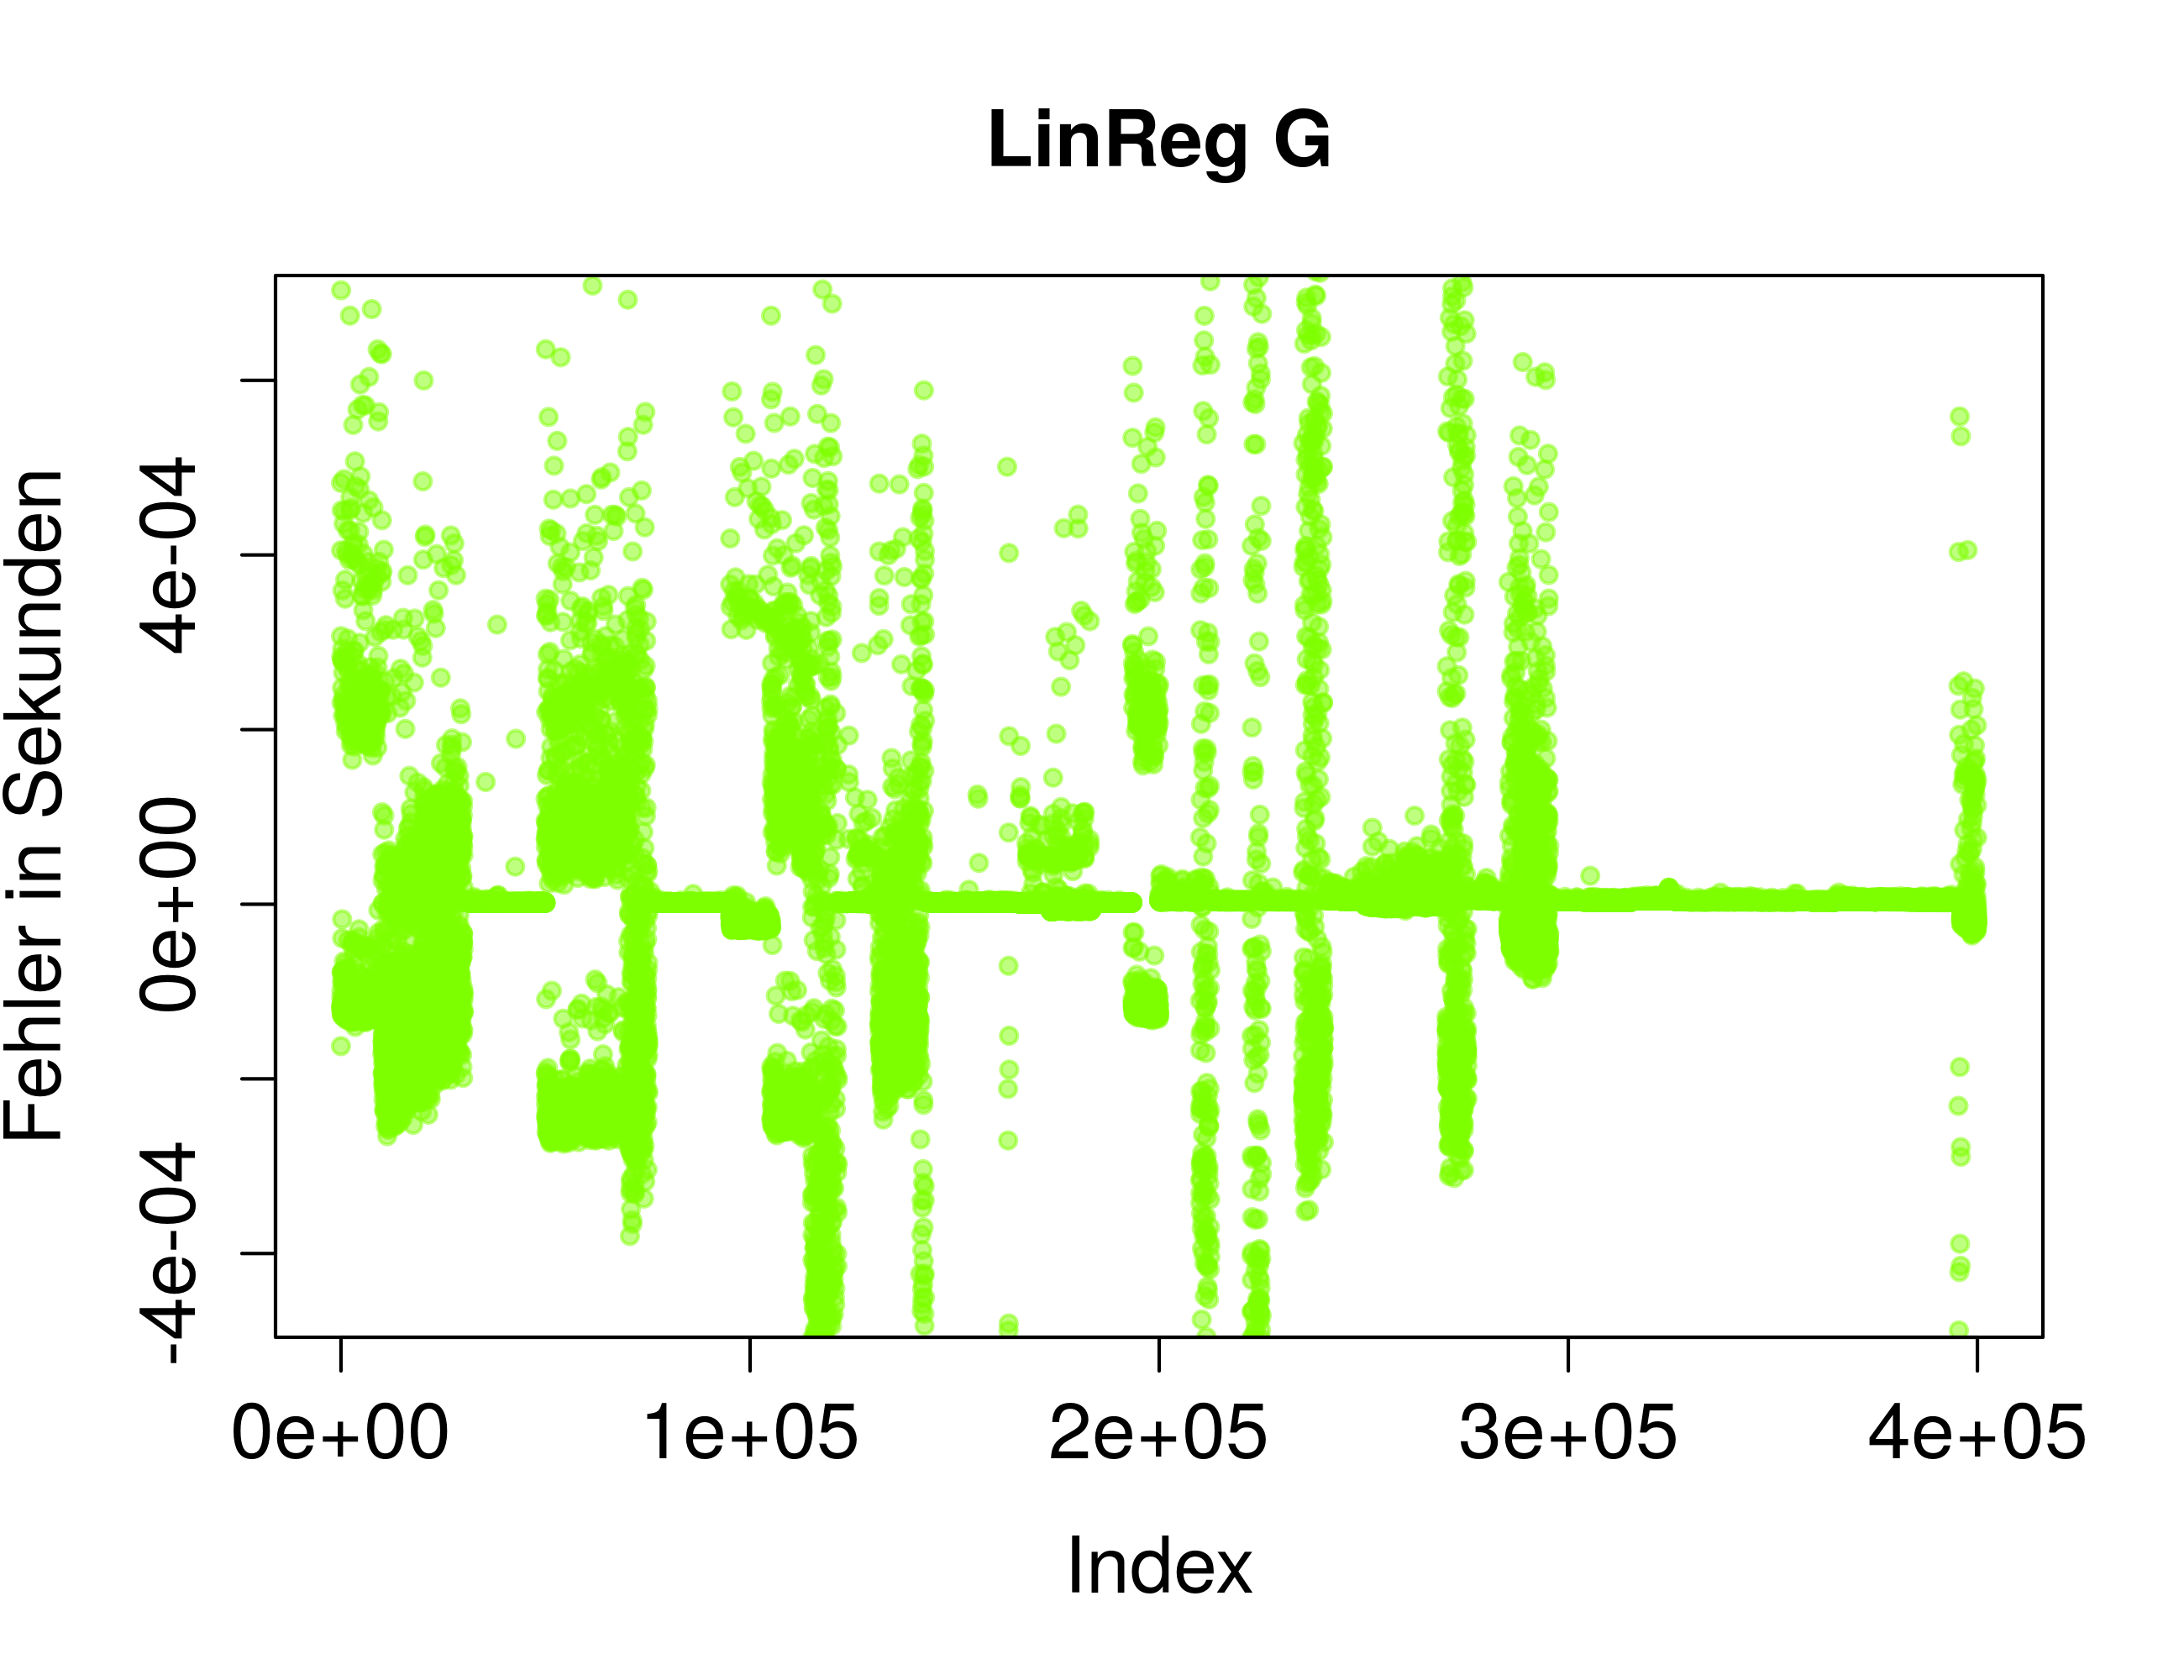
\includegraphics[width=.43\textwidth]{Bilder/Plots/error_class/exploration/rnd_linreg_classes_on_seq.png}
	}
	\subfloat[Sortiert nach Modellabweichung, alle Punkte gezeichnet]{
		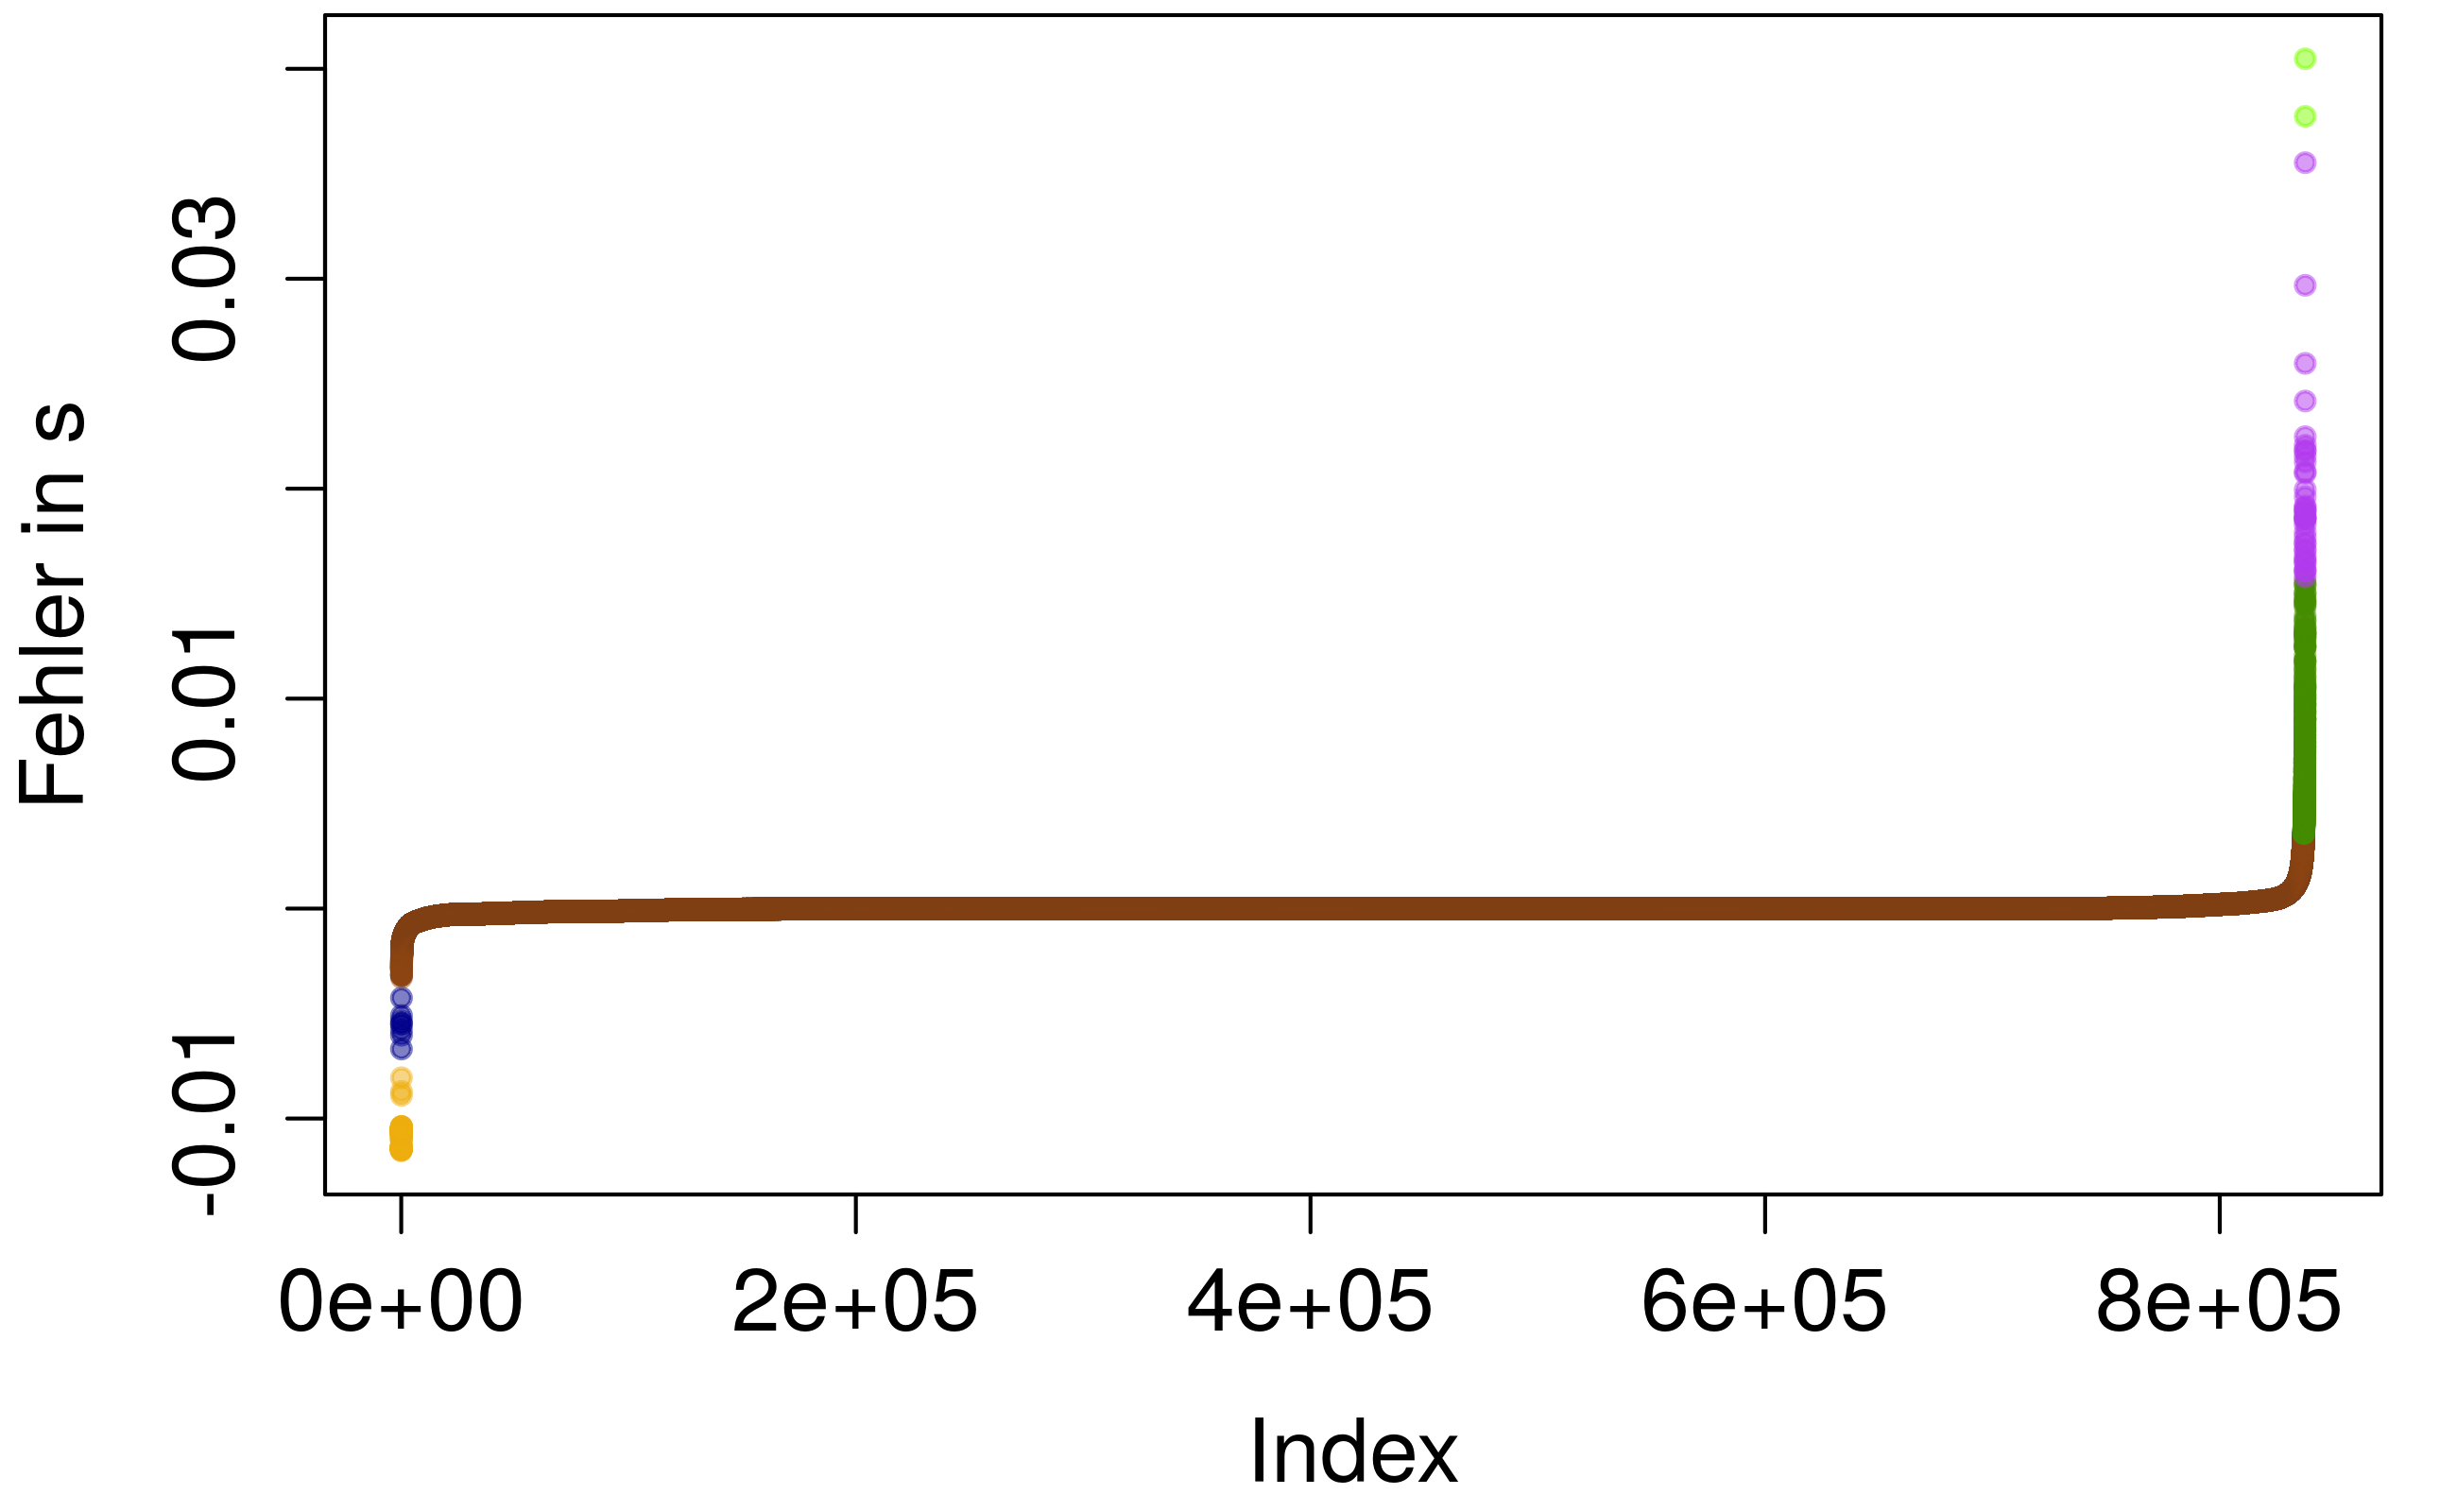
\includegraphics[width=.43\textwidth]{Bilder/Plots/error_class/exploration/rnd_linreg_classes_on_seq_sorted.png}
	}\\
	\subfloat[Klassen aus den sequentiellen Zugriffen $\text{}$ angewendet auf die randomisierten Messungen, sortiert nach Größe]{
		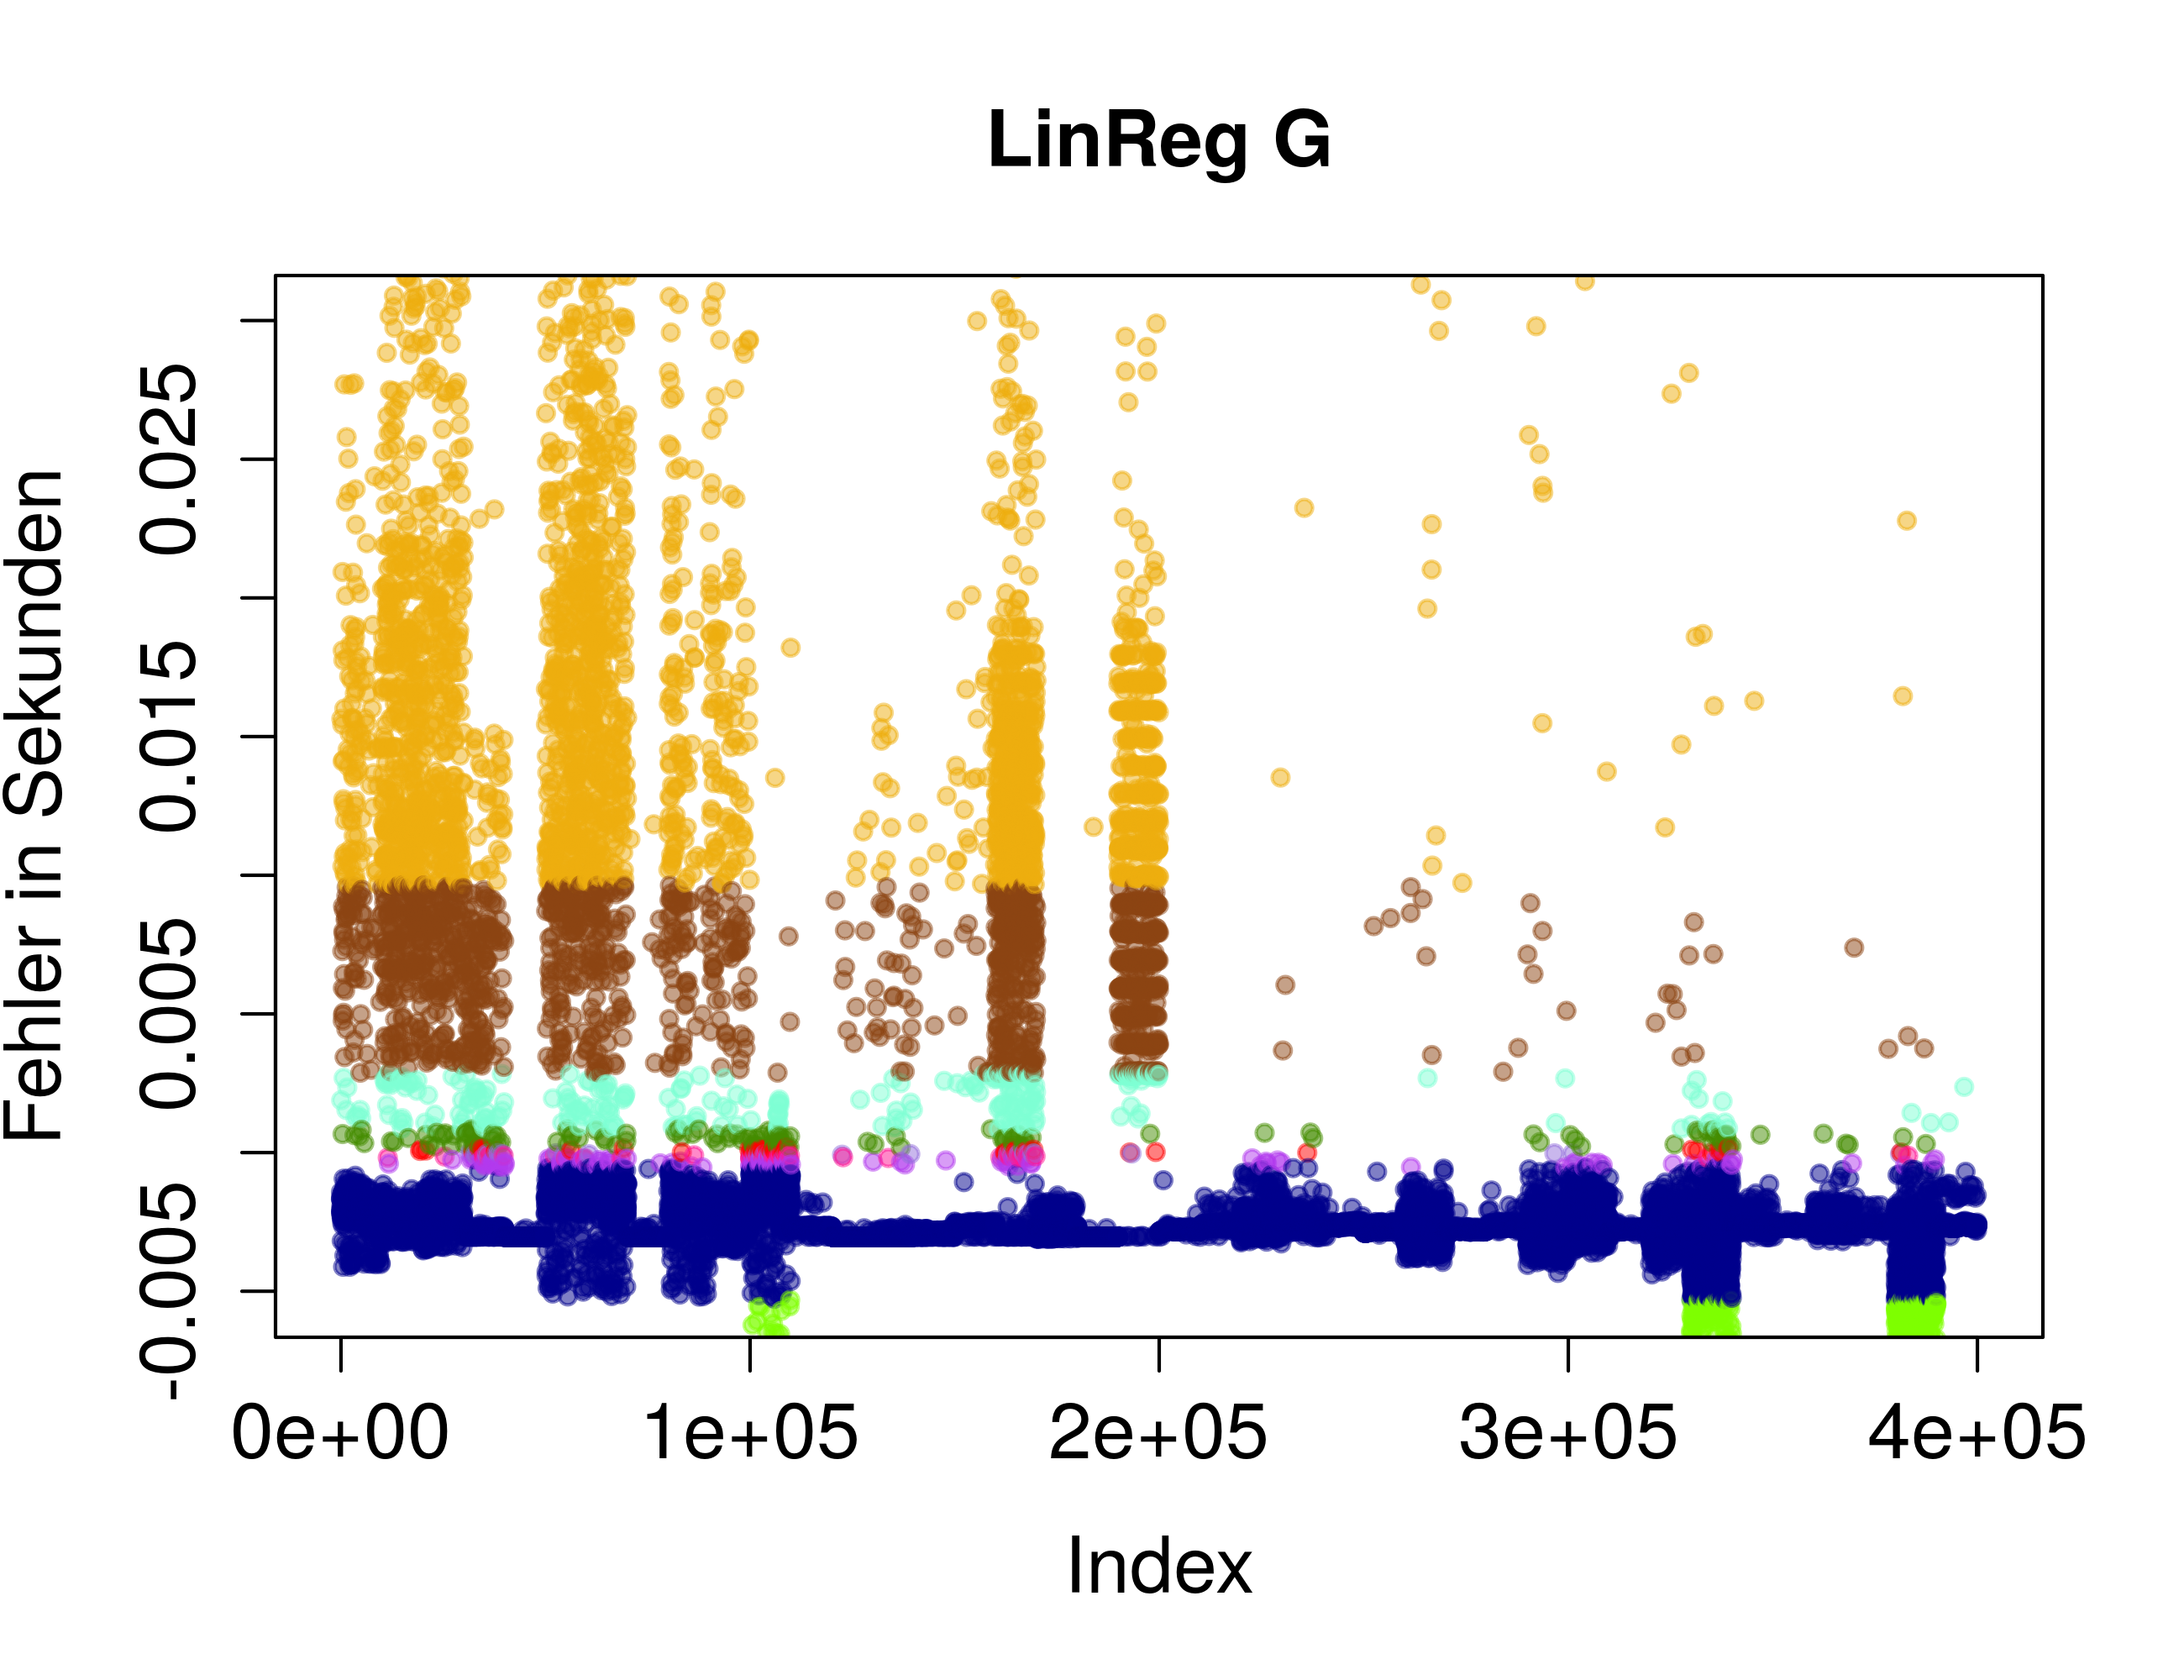
\includegraphics[width=.43\textwidth]{Bilder/Plots/error_class/exploration/seq_linreg_classes_on_rnd.png}
	}
	\subfloat[Sortiert nach Modellabweichung, alle Punkte gezeichnet]{
		\includegraphics[width=.43\textwidth]{Bilder/Plots/error_class/exploration/seq_linreg_classes_on_rnd_sorted.png}
	}
	\caption{Farblich markierte Fehlerklassen, unter Verwendung der Fehlerklassen, die aus aus dem jeweils anderen Datensatz stammen}
	\label{fig:error_classes_switched}
\end{figure} 

In den Tabellen \ref{tab:error_classes_switched} wurden die Fehlerklassen nach dem arithmetischen Mittel der Residuen (Durchschnitt) der enthaltenen Datenpunkte sortiert.
Zu jeder Fehlerklasse wird der abgedeckte Bereich angegeben, der sich von dem in ihm enthaltenen Datenpunkt mit dem kleinsten Fehler (Min) bis zu dem mit größten Fehler (Max) erstreckt. 
Desweiteren ist der mittlere Durchsatz in Byte pro Sekunde angegeben, der sich für die Cluster-Gruppen ergibt.
Zuletzt wird die Anzahl Datenpunkte angegeben, die sich in dem abgedeckten Bereich der Klasse befinden, zum einen für den Datensatz auf dem sie erstellt wurden und auch für den jeweils anderen Datensatz.

Für SEQ befinden sich mit vertauschten Fehlerklassen 836841 von von 837600 Punkten in der selben Klasse.
Dies ist die Klasse, die den geringsten Durchsatz hat und in der \textit{LinReg G} zuvor auf dem randomisierten Datensatz den größten Fehler gemacht hat.
Die Fehlerklassen von SEQ sind dagegen sogar recht gut zur Differenzierung der Datenpunkte auf RND nutzbar, wie in Tabelle \ref{tab:error_classes_switched} b) an den Werten für \textit{Zugeordnet auf rnd} zu entnehmen ist und auch in \ref{fig:error_class_clustering_rnd}c sichtbar ist.
Dies ist dem Umstand geschuldet, dass die Fehlerklassen auf den sequentiellen Daten in dem Bereich mit kleinem Fehler stark differenziert und die meisten Punkte sich auch auf RND dort befinden.
Für eine bessere Vorhersage der Messdaten würden sich diese Klassen auf beiden Datensätzen nicht eignen.
Auf SEQ, da sich praktisch alle Punkte in der selben Klasse befinden und auf RND, weil in den entscheidenden schlechteren Vorhersagen von \textit{LinReg G} keine Unterscheidung stattfindet.
Den mittleren Durchsätzen kann entnommen werden, dass die sich Größe des Fehlers umgekehrt proportional zum gemachten Durchsatz des E/A-Zugriffs verhält.
Für die sequentiellen Daten ist dieser Trend weniger ausgeprägt, als für die randomisierten. 
Der Zusammenhang zwischen mittlerem Residuum und mittlerem Durchsatz weist weiterhin auf die Beziehung von Fehlerklassen zu E/A-Pfaden hin.
Denn in guter Näherung sollte ein Pfad, der von den durchquerten Speichereinheiten und Netzwerken abhängt, einen spezifischen Durchsatz haben.
Dieser Durchsatz wird durch die langsamsten Einheiten auf dem Pfad geprägt.

\begin{table}
	\scriptsize
	\subfloat[Fehlerklassen aus \textit{LinReg G} auf SEQ]{
		\begin{tabular}{|r|r|r|r|r|r|r|}\hline%
			Klasse & mittlerer Durchsatz (B/s) & Min (s) & Durchschnitt (s) & Max (s) & Zugeordnet auf seq & Zugeordnet auf rnd \\\hline\hline
			\csvreader[late after line=\\\hline]%
			{CSV/error_class/seq_linreg_classes_on_rnd.csv}{tp=\tp,idx = \idx,rndcount=\rndcount,minerror=\minerror, meanerror = \meanerror, maxerror = \maxerror, seqcount = \seqcount}%
			{\idx & \tp & \minerror & \meanerror & \maxerror & \seqcount & \rndcount}%
		\end{tabular}
	}\\
	\subfloat[Fehlerklassen aus \textit{LinReg G} auf RND]{
		\begin{tabular}{|r|r|r|r|r|r|r|}\hline%
			Klasse & mittlerer Durchsatz (B/s) & Min (s) & Durchschnitt (s) & Max (s) & Zugeordnet auf rnd & Zugeordnet auf seq \\\hline\hline
			\csvreader[late after line=\\\hline]%
			{CSV/error_class/rnd_linreg_classes_on_seq.csv}{tp=\tp,idx = \idx, rndcount=\rndcount,minerror=\minerror, meanerror = \meanerror, maxerror = \maxerror, seqcount = \seqcount}%
			{\idx & \tp & \minerror & \meanerror & \maxerror & \rndcount & \seqcount}%
		\end{tabular}
	}
	\caption{LinReg-Fehlerklassen sortiert von kleinem zu großem Zentrum des Clusters (Durchschnittlicher Fehler). Einmal die Anzahl Punkte, die den Klassen auf dem Datensatz zugeordnet wurden, von dem sie auch stammen. Zudem die Anzahl Punkte, die den Klassen auf dem anderen Datensatz zugeordnet werden würden.}
	\label{tab:error_classes_switched}
\end{table}

Neben den Fehlerklassen, die aus der Modellabweichung von \textit{LinReg G} gewonnen wurden, gibt es noch die Fehlerklassen aus den Modellabweichungen von \textit{Tupel1}.
In Tabelle \ref{tab:error_classes_switched2} sind die gleichen Angaben, wie in \ref{tab:error_classes_switched} zu den Fehlerklassen angegeben. Zusätzlich steht in der Spalte \textit{Identisch}, welcher Anteil der Datenpunkte in den Clustern von \textit{LinReg G} und \textit{Tupel1} der selben Fehlerklasse zugewiesen wurden.
Insgesamt sind die Zuweisungen sehr ähnlich. Auf SEQ gibt es eine sehr große Übereinstimmung bei Klasse mit den meisten Datenpunkten, sodass insgesamt 90\% der gleiche Zuordnung stattfindet.
Auf RND stimmen die Zuweisungen zu vielen Klassen stärker überein, in der ausschlaggebenden Klasse allerdings nur um 80.5\%, sodass insgesamt 78\% identische Zuordnungen gemacht wurden.
Auch die abgedeckten Bereiche der Klassen sind denen von \textit{LinReg G} sehr ähnlich.

\begin{table}
	\makebox[\textwidth][c]{
		\scriptsize
		\subfloat[Fehlerklassen aus Tupel1 auf SEQ; insgesamt 90\% Übereinstimmung gegenüber \textit{LinReg G} bei der Klassenzuteilung]{
			\begin{tabular}{|r|r|r|r|r|r|r|r|}\hline%
				Klasse & mittlerer Durchsatz (B/s) & Min (s) & Durchschnitt (s) & Max (s) & Zugeordnet auf seq & Zugeordnet auf rnd & Identisch (\%) \\\hline\hline
				\csvreader[late after line=\\\hline]%
				{CSV/error_class/seq_linreg_classes_on_rnd_good.csv}{tp=\tp,idx = \idx, rndcount=\rndcount,minerror=\minerror, meanerror = \meanerror, maxerror = \maxerror, seqcount = \seqcount, equa = \equa}%
				{\idx & \tp & \minerror & \meanerror & \maxerror & \rndcount & \seqcount &\equa}%
			\end{tabular}
		}
	}\\
	\makebox[\textwidth][c]{
		\scriptsize
		\subfloat[Fehlerklassen aus Tupel1 auf RND; insgesamt 78\% Übereinstimmung gegenüber \textit{LinReg G} bei der Klassenzuteilung]{
			\begin{tabular}{|r|r|r|r|r|r|r|r|}\hline%
				Klasse & mittlerer Durchsatz (B/s) & Min (s) & Durchschnitt (s) & Max (s) & Zugeordnet auf rnd & Zugeordnet auf seq & Identisch (\%) \\\hline\hline
				\csvreader[late after line=\\\hline]%
				{CSV/error_class/rnd_linreg_classes_on_seq_good.csv}{tp=\tp,idx = \idx, rndcount=\rndcount,minerror=\minerror, meanerror = \meanerror, maxerror = \maxerror, seqcount = \seqcount, equa = \equa}%
				{\idx & \tp & \minerror & \meanerror & \maxerror & \rndcount & \seqcount &\equa}%
			\end{tabular}
		}
	}
	\caption{Analyse der Tupel1-Fehlerklassen parallel zur vorherigen Tabelle}
	\label{tab:error_classes_switched2}
\end{table}
\clearpage

\section{Leistungsvorhersage}
Nachdem die Messdaten untersucht worden sind werden nun die verschiedenen Modelle auf die Daten angewendet. Die Modellabweichungen gegenüber den tatsächlich gemessen Werten können dazu genutzt werden weitere Aussagen über die Beschaffenheit der Messdaten zu machen und das E/A-System kann letztendlich besser verstanden werden.

\subsection{Analyse der trivialen Modelle}

Die Ergebnisse der in \ref{impl:modelle} beschriebenen trivialen Modelle sind in \ref{tab:triv} zu sehen. Die Spalte \textit{Typ} gibt an, ob das Modell auf den aggregierten Daten (agg) oder auf den individuellen Messungen (Ind) in Zeitreihe gelernt wurden.
Eine positive Beobachtung in den Ergebnissen auf SEQ ist zunächst, dass alle Metriken einen ähnlichen Trend der  Modelle aufzeichnen.
Das gilt im Wesentlichen auch für RND, jedoch hat das Modell \textit{Median} einen sehr hohen maximalen Fehler. Dies führt entsprechend zu einem vergleichsweise hohen RMQA-Wert, obwohl der relative arithmetische Fehler noch recht gering ist.
Wie erwartet (\textbf{ABSCHNITT}) sind die Vorhersagen auf dem randomisierten Datensatz schwieriger zu machen, sodass die Modellabweichungen wesentlich höher sind.
Dies gilt insbesondere für die Modelle, die auf linearer Regression basieren.
Eine Ausnahme bilden die Fehlerklassen-Modelle, die Modelle können weiterhin sehr gute mittlere Vorhersagen treffen, einige Messungen können auf RND sehr schlecht vorhergesagt werden, sodass RMax und RMQA höher als bei sequentiellen Datensatz sind.

Allgemein sind die Ergebnisse bereits überraschend gut.
Die Modelle \textit{Median} und \textit{LinReg G} haben eine durchschnittliche Modellabweichung von 0.6-0.8 Millisekunden gegenüber den sequentiell durchgeführten Zugriffen und 16-44 Millisekunden gegenüber den zufälligen Dateizugriffen.
Ein durchschnittlicher relativer Fehler von $6-7\%$ auf den sequentiellen Messungen bzw. $8-12\%$ auf den randomisierten Messungen durch die Modelle, die Fehlerklassen ausnutzen, deutet daraufhin, dass die Vorgänge im E/A-System im Wesentlichen korrekt repräsentiert werden.
Ob über eine größere Messreihe ein wesentlich geringerer durchschnittlicher Fehler als einige Prozentpunkte überhaupt erreicht werden kann, ist fraglich, da das Messrauschen durch unvorhersehbare Ereignisse sowohl auf System-, als auch Bauteilebene, in diesen Bereichen eine zu große Bedeutung zukommt.
Die Modelle mit linearer Regression führen auf SEQ auch bereits zu zufriedenstellenden Ergebnissen, während sie auf RND kaum sinnvolle Vorhersagen zu machen scheinen.
\textit{Median} hat jeweils eine akzeptable Leistung, während \textit{Durchschnitt} durchweg ungenügende Residuen aufweist.
Interssant ist, dass Modelle mit linearer Regression auf dem sequentiellen Datensatz eine zufriedenstellende Vorhersage machen, während die Vorhersage auf dem randomisierten Messungen teilweise kaum besser als das Durschnitts-Modell ist. 
Das Modell, das immer die Durchschnittsdauer vorhersagt ist als absolute untere Grenze für angewendete Modelle zu verstehen, da hier praktisch keine Expertise über die Daten eingeht. 
Tatsächlich erreicht dieses Modell die schlechtesten Werte für die Fehlermetriken in beiden Testfällen. Die Ansätze der rechenintensiven halten diesem Anspruch also stand und sind soweit gerechtfertigt.
Aufgrund des geringen Nutzen der Attribute Abstand und OpTyp für die lineare Regression wird im Folgenden nur das Modell über die Zugriffsgröße betrachtet.
Da \textit{LinReg G} auf SEQ wesentlich bessere Werte mit Eingabedaten als individuelle Messungen hat, und die Leistung für \textit{Agg} und \textit{Ind} auf RND in etwa gleichauf sind, wird nur \textit{LinReg G} mit Zeitreihen-Daten berücksichtigt.

Die geringen Unterschiede in den Modellabweichungen von \textit{Median LinReg-FK} und \textit{Median Tupel1-FK}, sowie der in Tabelle \ref{tab:error_classes_switched2} festgestellten sehr ähnlichen Struktur beider Fehlerklassenzuweisungen rechtfertigen es, im Folgenden nur noch die Modelle zu beachten, die sich auf \textit{LinReg G}-Fehlerklassen beziehen.
(\textbf{Tupel1 FK in Tupel1 lernen ist problematisch ..})

\begin{table}
	\scriptsize
	\subfloat[cached-off0-seq]{
		\begin{tabular}{|r|r|r|r|r|r|r|}\hline%
			Modell & MAF (s)  & RMAF (\%) & RMQA (\%) & RQ3 (\%) & RMax (\%) & Typ \\\hline\hline
			\csvreader[late after line=\\\hline]%
			{CSV/baselines/latex_baseline_seq_results.csv}{Modell=\Model,MAF=\MAF,RMAF=\RMAF, RMQA = \RMQA, Q3 = \Q3, Max = \Max, Typ = \Typ}%
			{\Model & \MAF & \RMAF & \RMQA & \Q3 & \Max & \Typ}%
		\end{tabular}
	} \\
	\subfloat[cached-off0-rnd]{
		\begin{tabular}{|r|r|r|r|r|r|r|}\hline%
			Modell & MAF (s)  & RMAF (\%) & RMQA (\%) & RQ3 (\%) & RMax (\%) & Typ \\\hline\hline
			\csvreader[late after line=\\\hline]%
			{CSV/baselines/latex_baseline_rnd_results.csv}{Modell=\Model,MAF=\MAF,RMAF=\RMAF, RMQA = \RMQA, Q3 = \Q3, Max = \Max, Typ = \Typ}%
			{\Model & \MAF & \RMAF & \RMQA & \Q3 & \Max & \Typ}%
		\end{tabular}
	}
	\caption{Ergebnisse der trivialen Modelle}
	\label{tab:triv}
\end{table}
Um genauer zu verstehen, wie die trivialen Modelle die Messdaten annähern, ist es notwendig sich die vorhergesagten Werte gegenüber den tatsächlichen Werten anzuschauen.
Wie zuvor sind die Messdaten nach Zugriffsgröße und Operationstyp sortiert. 
Auf den Graphen zu den sequentiellen Daten \ref{fig:zeit_baselines_seq} lässt sich recht gut die Qualität der Modelle anhand der Stärke der Differenzierung zwischen den Zugriffsgrößen erkennen.
Während bei \textit{Durchschnitt} gar nicht differenziert wird, kann \textit{Median} natürlich alle Größen unterscheiden. 
\textit{LinReg G} kann einige Größen unterscheiden, versagt jedoch bei den kleinsten Zugriffen.
Sehr schön ist in  \ref{fig:zeit_baselines_seq}b die Problematik des linearen Modells zu beobachten, die aufwendigeren Zugriffe können recht gut als linear von der Zugriffsgröße abhängig modelliert werden, für die kleineren Größen gilt dies jedoch nicht mehr.
Das Modell mit Kenntnis von Fehlerklassen kann innerhalb einer Zugriffsgröße weitere Differenzierungen machen und erreicht entsprechend die besten Fehlerwerte.
Besonders die höheren Zugriffsgrößen können besser von \textit{Median LinReg-FK} modelliert werden. Das passt zu dem Bild, das wir von der Struktur der Fehlerklassen gewonnen haben. Auf SEQ wird fast ausschließlich für aufwendigere Zugriffe eine Aufteilung durch die Fehlerklassen vorgenommen. 
\begin{figure}
	\subfloat[Modell \textit{Durchschnitt}]{
		\includegraphics[width=.43\textwidth]{Bilder/Plots/baselines/plot_seq_mean_performance.png}
	}
	\hfill
	\subfloat[Modell \textit{LinReg G}; Achtung: verschobene Y-Achse]{
		\includegraphics[width=.43\textwidth]{Bilder/Plots/baselines/plot_seq_linreg_Size.png}
	}\\
	\subfloat[Modell \textit{Median}]{
		\includegraphics[width=.43\textwidth]{Bilder/Plots/baselines/plot_seq_median_Duration_aggregated.png}
	}
	\hfill
	\subfloat[Modell \textit{Median LinReg-FK}]{
		\includegraphics[width=.43\textwidth]{Bilder/Plots/baselines/plot_seq_median_Duration_with_linreg_error_class_aggregated.png}
	}
	\caption{Triviale Modelle auf SEQ; in Blau die vom Modell vorhergesagten Werte; lesende Zugriffe in dunkelgrau schreibende in hellgrau}
	\label{fig:zeit_baselines_seq}
\end{figure} 
Grob ergibt sich auch ein ähnliches Bild auf dem Datensatz mit zufälligen Dateizugriffen. Umso größer die Verteilung der Vorhersagen, desto besser das Modell  (\ref{fig:zeit_baselines_rnd}).
Die Probleme der linearen Regression werden auch hier sichtbar, da einer Größe genau ein Funktionswert zugewiesen wird, ist die Abstraktionsmöglichkeit für den randomisierten Datensatz, mit stärkerer Varianz der Laufzeiten, nicht mehr ausreichend.
Tatsächlich ist eine starke Ähnlichkeit der linearen Regression zum Durchschnitts-Modell erkennbar. Nur für die höheren Zugriffsgrößen, ähnlich wie bei SEQ, kann eine bessere Modellierung durch die Regression vorgenommen werden.

Um die Leistungsunterschiede zwischen \textit{Median} und den Fehlerklassen-Modellen zu erkennen versagt die Zeitreihe.
\textbf{Im sortierten Graphen ist dagegen klar zu sehe}n, dass \textit{Median} eine stärkere Streuung bei der Vorhersage der langsameren Datenpunkte aufweist. 
\begin{figure}
	\subfloat[Modell \textit{Durchschnitt}]{
		\includegraphics[width=.43\textwidth]{Bilder/Plots/baselines/plot_rnd_mean_performance.png}
	}
	\hfill
	\subfloat[Modell \textit{LinReg G}]{
		\includegraphics[width=.43\textwidth]{Bilder/Plots/baselines/plot_rnd_linreg_Size.png}
	}\\
	\subfloat[Modell \textit{Median}]{
		\includegraphics[width=.43\textwidth]{Bilder/Plots/baselines/plot_rnd_median_Duration_aggregated.png}
	}
	\hfill
	\subfloat[Modell \textit{Median LinReg-FK}]{
		\includegraphics[width=.43\textwidth]{Bilder/Plots/baselines/plot_rnd_median_Duration_with_linreg_error_class_aggregated.png}
	}
	\caption{Triviale Modelle auf RND; in Blau die vom Modell vorhergesagten Werte; lesende Zugriffe in dunkelgrau schreibende in hellgrau}
	\label{fig:zeit_baselines_rnd}
\end{figure} 
\begin{figure}
	\subfloat[Modell \textit{Median}]{
		\includegraphics[width=.43\textwidth]{Bilder/Plots/baselines/plot_rnd_DurationToPredSorted_median_Duration_aggregated.png}
	}
	\hfill
	\subfloat[Modell \textit{Median LinReg-FK}]{
		\includegraphics[width=.43\textwidth]{Bilder/Plots/baselines/plot_rnd_DurationToPredSorted_median_Duration_with_linreg_error_class_aggregated.png}
	}
	\caption{Triviale Modelle auf RND sortiert nach Laufzeit; jeder 250te Punkt gezeichent, in Blau die vom Modell vorhergesagten Werte}
	\label{fig:zeit_baselines_sorted_rnd}
\end{figure} 

Erneut kann untersucht werden, wie die unterschiedliche Qualität der Vorhersagen zu Stande kommt, indem kleinere Ausschnitte der Modell-Prognosen betrachtet werden.
In den Graphen in \ref{fig:densities_baselines_seq} ist die Dichte der Laufzeiten für jeweils ein spezifisches Attribut-Set dargestellt. Der angegebene Fehler ist der relative arithmetische Fehler des Modells auf dem Set.
Es gibt jeweils $N$ Messungen mit den Attributen aus diesem Set.
In \ref{fig:densities_baselines_seq}a ist die Vorhersage vom Modell \textit{Durchschnitt} zu dem Attribut-Set zu sehen, das von dem Modell mit am Besten modelliert wurde.
Die Vorhersage ist nicht sehr genau, der vom Modell geschätzte Wert ist wesentlich näher am 0.1 Quantil, als am tatsächlichen Mittelwert.
Die Vorhersage mit dem geringsten Fehler von \textit{LinReg G} ist in \ref{fig:densities_baselines_seq}b zu sehen.
Der vorhergesagte Wert befindet sich ziemlich genau am Maximum der Dichtefunktion. Entsprechend sagt dieses Modell für eine möglichst große Anzahl Messungen den richtigen Wert voraus. 
%Das im Modell \textit{Median} eben gerade der Median der Attribut-Sets vorhergesagt wird, statt z.B. dem arithmetischen Mittel, kommt in \ref{fig:densities_baselines_seq}c zu tragen. Würde das Modell das arith. Mittel vorhersagen, wäre die Vorhersage für dieses Set exakt an der Stelle der schwarzen Markierung. Dadurch wäre der Wert des Fehlermaßes  RMAF noch geringer, denn durch die Ausläufer der Messungen dieses Sets zu höheren Laufzeiten wird das arith. Mittel im Graph nach rechts gezogen. Stattdessen wird nun durch den Median ein Großteil der Messungen genauer vorhergesagt, nämlich die Messungen zu den Aufrufen mit der typischen Laufzeit, während die Ausreißer vernachlässigt werden.
Die Vorhersage von \textit{Median LinReg-FK} liegt auf dem in \ref{fig:densities_baselines_seq}c dargestellten Attribut-Set ziemlich genau auf dem Wert des arithmetischen Mittels, sodass der arithmetische Fehler hier gerade minimal wird.
Als letztes Beispiel soll der Verlauf der Laufzeit-Dichte eines Attribut-Sets gezeigt werden, zu dem das Modell \textit{Median} eine seiner größten Modellabweichungen hat.
Interessanterweise sind die Residuen für dieses Attribut-Set sehr groß, dabei ist der Vorhergesagte Wert des Modells in direkter Nähe des tatsächlichen arith. Mittelwerts.
Ein Modell, dass für alle Messungen eines Sets den selben Wert vorhersagt, kann dementsprechend zu den gemachten Messungen nicht immer kleine Modellabweichungen erreichen.
Eine weitere Unterscheidung von Messungen innerhalb eines Sets kann mit den verfügbaren Messdaten allerdings nur durch eine Betrachtung der zeitlichen Abhängigkeit des E/A-Aufrufs von den vorherigen gelingen. 
Alternativ kann ein Ansatz, wie die Fehlerklassen zur besseren Modellierung verwendet werden, dies ist aber natürlich \textit{unfair}, da in den Klassen Informationen über die tatsächliche Laufzeit der E/A-Aufrufe stecken.
 
 \begin{figure}
 	\centering
 	\subfloat[Modell \textit{Durchschnitt}; Mitt.-Fehler: 20.77\%, N = 29997, Zugriffsgröße = Delta-Abstand: 512KiB, OpTyp: W]{
 		\includegraphics[width=.43\textwidth]{Bilder/Plots/baselines/Dichten/plot_density_best_mean_performance.png}
 	}
 	\subfloat[Modell \textit{LinReg G}; Mitt.-Fehler: 6.74\%, N: 29997, Zugriffsgröße = Delta-Abstand: 64KiB, OpTyp: W]{
 		\includegraphics[width=.43\textwidth]{Bilder/Plots/baselines/Dichten/plot_density_best_linreg_Size.png}
 	}\\
 	\subfloat[Modell \textit{Median LinReg-FK}; Mitt. - Fehler: 2.6\%, N:3837, Zugriffsgröße = Delta-Abstand: 8MiB, OpTyp: W]{
 		\includegraphics[width=.43\textwidth]{Bilder/Plots/baselines/Dichten/plot_density_best_median_Duration_with_linreg_error_class_aggregated.png}
 	}
 	\subfloat[Modell \textit{Median}; Mitt. - Fehler: 68.65\%, N: 29997, Zugriffsgröße = Delta-Abstand: 512KiB, OpTyp: W]{
 		\includegraphics[width=.43\textwidth]{Bilder/Plots/baselines/Dichten/plot_density_worst_median_Duration_aggregated.png}
 	} 
 	\caption{Laufzeit-Dichte einiger trivialer Modelle auf SEQ; 90\% der Werte sind größer als die grüne, 10\% sind größer als die pinke Linie, die mittlere Dauer entspricht der schwarzen Linie, die blaue Linie ist die mittlere Vorhersage des Modells für dieses Set}
 	\label{fig:densities_baselines_seq}
 \end{figure} 

\clearpage

\subsection{Analyse der höheren Modelle}

Die Analyse zu den aufwendigeren Modellen, die auf neuronalen Netzen basieren, ist dreigeteilt. 
Zunächst eine kurze Betrachtung der Struktur des erfolgreichsten neuronalen Netzes zu dem Modell. 
Dann die Untersuchung der Qualität der Vorhersagen auf SEQ und RND.
Und zuletzt wird für die Anwendung auf SEQ zusätzlich die Ausreißer-Vorhersage genauer studiert.
Es wird zu jedem Modell das neuronale Netz angegeben, das bei der Untersuchung des Parameterraums gefunden wurde und den geringsten RMQA-Wert erzielt hat.
Informationen über die Struktur der Netze und den Aufwand des Trainingsprozesses finden sich in \ref{tab:model-stats}. Im Detail sind dies die Anzahl der verdeckten Schichten, sowie die Anzahl Neuronen, die jede Schicht enthält, die Anzahl Iterationen, die der Algorithmus gebraucht hat, bis der Schwellenwert für die Konvergenz erreicht war, und die Trainingsdauer, also wie lange die Berechnung des Netzes tatsächlich gedauert hat.
In Tabelle \ref{tab:results} sind für alle NN-Modelle die Werte der verschiedenen Fehlermetriken angegeben, zusätzlich sind zum Vergleich die Basis-Modelle \textit{Durchschnitt}, \textit{LinReg G} angewendet auf individuelle Messungen und \textit{Median LinReg-FK} aufgelistet.
Die Tabelle \ref{tab:outlier} wird für die Analyse der Ausreißer-Vorhersage betrachtet.

\begin{table}
	\scriptsize
	\subfloat[NN-Modelle auf SEQ]{
		\begin{tabular}{|r|r|r|r|r|}\hline%
			Modell & verdeckte Schichten & Neuronen & Iterationen & Trainingsdauer (s) \\\hline\hline
			\csvreader[late after line=\\\hline]%
			{CSV/models/latex_seq_net-stats.csv}{Modell=\Model,verdeckteSchichten=\verdeckteSchichten,Neuronen=\Neuronen, Iterationen = \Iterationen, Trainingsdauer = \Trainingsdauer}%
			{\Model & \verdeckteSchichten & \Neuronen & \Iterationen & \Trainingsdauer}%
		\end{tabular}
	} \\
	\subfloat[NN-Modelle auf RND]{
		\begin{tabular}{|r|r|r|r|r|}\hline%
			Modell & verdeckte Schichten & Neuronen & Iterationen & Trainingsdauer (s) \\\hline\hline
			\csvreader[late after line=\\\hline]%
			{CSV/models/latex_rnd_net-stats.csv}{Modell=\Model,verdeckteSchichten=\verdeckteSchichten,Neuronen=\Neuronen, Iterationen = \Iterationen, Trainingsdauer = \Trainingsdauer}%
			{\Model & \verdeckteSchichten & \Neuronen & \Iterationen & \Trainingsdauer}%
		\end{tabular}
	}
	\caption{Informationen über die erfolgreichsten Neuronalen Netze}
	\label{tab:model-stats}
\end{table}

\begin{table}
	\scriptsize
	\makebox[\textwidth][c]{
		\subfloat[Fehlermetriken auf SEQ]{
			\begin{tabular}{|r|r|r|r|r|r|r|r|r|}\hline%
				Modell & MAF (s) & RMAF Avg (\%) & RMAF Train (\%) &  RMAF (\%) & RMQA (\%) & RQ3 (\%) & RMax (\%) & Bereich (\%) \\\hline\hline
				\csvreader[late after line=\\\hline]%
				{CSV/models/latex_seq_results.csv}{Modell=\Model,MAF=\MAF,RMAF=\RMAF, RMQA = \RMQA, Q3 = \Q3, Max = \Max,RMAFTraining = \RMAFTraining, Bereich = \Bereich, RMAFavg = \RMAFavg}%
				{\Model & \MAF & \RMAFavg & \RMAFTraining & \RMAF & \RMQA & \Q3 & \Max & \Bereich}%
			\end{tabular}
		}
	}\\
	\makebox[\textwidth][c]{
		\subfloat[Fehlermetriken auf RND]{
			\begin{tabular}{|r|r|r|r|r|r|r|r|r|}\hline%
				Modell & MAF (s) & RMAF Avg (\%) &  RMAF Train (\%) & RMAF (\%) & RMQA (\%) & RQ3 (\%) & RMax (\%) & Bereich (\%) \\\hline\hline
				\csvreader[late after line=\\\hline]%
				{CSV/models/latex_rnd_results.csv}{Modell=\Model,MAF=\MAF,RMAF=\RMAF, RMQA = \RMQA, Q3 = \Q3, Max = \Max,RMAFTraining = \RMAFTraining, Bereich = \Bereich, RMAFavg = \RMAFavg}%
				{\Model & \MAF & \RMAFavg & \RMAFTraining & \RMAF & \RMQA & \Q3 & \Max & \Bereich}%
			\end{tabular}
		}
	}
	\caption{Ergebnisse der NN-Modelle und einiger Basis-Modelle}
	\label{tab:results}
\end{table}

\begin{table}
	\scriptsize
	\subfloat{
	\begin{tabular}{|r|r|r|r|r|r|r|}\hline%
		Modell & Q0.1 RMAF (\%) &Q0.1 RMQA (\%) & Q0.9 RMAF (\%) & Q0.9 RMQA (\%) & TP (\%) & FP (\%) \\\hline\hline
		\csvreader[late after line=\\\hline]%
		{CSV/models/latex_seq_outlier.csv}{Modell=\Model,QRMAF=\QRMAF,QRMQA=\QRMQA, LRMAF = \LRMAF, LRMQA = \LRMQA, Korrekt = \Korrekt, FalschPositiv = \FalschPositiv}%
		{\Model & \QRMAF & \QRMQA & \LRMAF & \LRMQA & \Korrekt & \FalschPositiv}%
	\end{tabular}
	}
	\caption{Informationen über die Ausreißervorhersage der NN-Modelle auf SEQ}
	\label{tab:outlier}
\end{table}

Als erstes wird das Modell \textit{Tupel1} untersucht. 
Das erfolgreichste neuronale Netz des Modells auf den sequentiellen Daten hat 12 verdeckte Schichten mit jeweils 8 Neuronen, es wurde über 24 Minuten in 1444 Iterationen entwickelt.
Trotz der höheren Varianz der Messdaten auf RND kommt das Modell hier mit 4 verdeckten Schichten mit 5 Neuronen aus, zudem wurde es schneller berechnet. Da die Leistungswerte des Modells gleichzeitig schlechter sind, scheint die Modellierung für dieses Problems nicht so erfolgreich zu sein, sodass ein simples abstrakteres Netz einem Komplexeren überlegen ist, das versuchen würde, die Datenstruktur detailreicher abzubilden.
Das Modell scheint stärker von der Tiefe der Schichten des neuronalen Netzes zu profitieren, als an der Anzahl Neuronen. 

Zu den sequentiell durchgeführten Messungen kann das Modell gut zwischen den Zugriffsgrößen und Operationstypen differenzieren (\ref{fig:tupel1_on_seq}a ). Recht zuverlässlich werden die Laufzeit-Häufungen zu den verschiedenen Attribut-Sets mit einem Wert innerhalb der Häufung approximiert.
Innerhalb eines Attribut-Sets kann das Modell jedoch keine weitere Differenzierung durchführen.
Stattdessen wird für eine Häufung immer der selbe Wert vorhergesagt.
Das zeigt sich auch am Wert für \textit{Bereich}, der angibt wie viele Vorhersagen zwischen den Quantilen 0.1 und 0.9 der Laufzeit des Attribut-Sets gelandet sind. Da das Modell nur eine Art Mittelwert vorhersagt, ist der Wert für \textit{Bereich} folgerichtig bei 100\%.
Dieses Verhalten entspricht dem des Basis-Modells \textit{Median}, tatsächlich ist der entsprechende Graph \ref{fig:zeit_baselines_rnd}c mit dem zu \textit{Tupel1} kaum zu unterscheiden.
Auch die Leistungswerte sind vergleichbar. Während \textit{Tupel1} einen etwas besseren RMQA mit 22\% zu 24\% hat, hat \textit{Median} mit einem RMAF von 11.1\% gegenüber 14.1\% leicht die Nase vorn. 
Dieses ähnliche Verhalten entspricht auch der Modellierung. \textit{Tupel1} stehen keine Informationen zur Unterscheidung der Attribut-Sets zur Verfügung, sodass intern ein möglichst guter Mittelwert zur Laufzeit jedes Sets gebildet werden muss. Dies gelingt \textit{Tupel1} mit dem kleinen Trainingsdatensatz in etwa genauso gut, wie \textit{Median} mit Kenntnis sämtlicher Messungen.
Der Modellierung entsprechend macht \textit{Tupel1} ungenaue Vorhersagen für Attribut-Sets, mit
großer Varianz in den Zugriffszeiten. 
Dies lässt sich in \ref{fig:tupel1_seq}c an der Markierung der nach oben gestreuten Laufzeiten erkennen.
Die besten Vorhersagen werden für Messungen gemacht, die möglichst der mittleren Dauer ihres Attribut-Sets entsprechen.
Das entwickelte neuronale Netz zeigt sich sehr zuverlässlich. Der \textit{RMAF} auf den Trainingsdatensatz und der durchschnittliche \textit{RMAF} über identische Netze ist sehr nah am \textit{RMAF} des betrachteten Netz.

\begin{figure}
	\centering
	\subfloat[Vorhersage der Laufzeiten]{
		\includegraphics[width=.43\textwidth]{Bilder/Plots/models/plot_onlyPred_tuple1_Duration_seq.png}
	}
	\hfill
	\subfloat[Vorhersagen der beiden Quantile 0.1 in grün und 0.9 in rot]{
		\includegraphics[width=.43\textwidth]{Bilder/Plots/models/plot_tuple1_Duration_seq.png}
	}\\
	\subfloat[Laufzeiten die mit höchster relativer Modellabweichung vorhergesagt wurden in rot]{
		\includegraphics[width=.43\textwidth]{Bilder/Plots/models/plot_biggest1_errors_tuple1_Duration_seq.png}
	}
	\hfill
	\subfloat[Laufzeiten geringster relativer Modellabweichung in grün]{
		\includegraphics[width=.43\textwidth]{Bilder/Plots/models/plot_smallest1_errors_tuple1_Duration_seq.png}
	}
	\caption{Modell \textit{Tupel1} auf SEQ}
	\label{fig:tupel1_seq}
\end{figure} 

Bei der Leistungsvorhersage auf cached-off0-rnd setzt sich Tupel1 mit 45\% RMAF und 122\% RMQA nun wesentlich vom linearen Modell mit 5019.1\% und 13188\% ab. Hier war LinReg G nicht mehr in der Lage die Häufungspunkte korrekt zu differenzieren. Tupel1 hingegen modelliert alle Häufungen korrekt (\ref{fig:tupel1_on_rnd}). Dadurch dass die Häufungen bei den randomisierten Messungen nicht mehr alle dem selben Attribut-Set angehören, sondern sich durch die Zugriffsort in der Datei unterscheiden, hat Tupel1 Informationen, um innerhalb einer Häufung verschiedene Vorhersagen zu treffen. Die Abhängigkeit der Laufzeit von Delta-Abstand ist jedoch sehr gering, sodass sich die Varianz der Vorhersagen in Grenzen halten. Die Stärken und Schwächen des Modells liegen
in den selben Bereichen, wie bei den sequentiellen Messungen.\\
Das Unvermögen innerhalb eines Attribut-Sets zu unterscheiden spiegelt sich auch darin wieder, dass 100\% der Vorhersagen von Tupel1 auf cached-off0-seq zwischen den tatsächlichen 0.1 und 0.9 Quantil des Sets liegt, idealerweise wenn alle Ausreißer richtig erkannt werden würden, wäre dieser Wert bei 80\%. Entsprechend sagt das Modell keine Ausreißer voraus, sodass TP und FP bei 0\% liegen. Auf cached-off0-rnd sind diese Werte nicht sehr Ausdrucksstark, denn zu jedem Attribut-Set gibt es jeweils nur ein bis drei Messungen, sodass die Quantile recht willkürlich sind.
Wie erwartet fällt die Vorhersage der Quantile auf cached-off0-seq leicht. Dort gibt es bloß 76 verschiedene Attribut-Sets, das Netz muss die entsprechenden Werte bloß \glqq merken\grqq{} und richtig zuordnen. Dies gelingt dem Netz mit wenigen Prozent Abweichung. 
Auf cached-off0-rnd dagegen gibt es 260 000 unterschiedliche Attribut-Sets, sodass das Netz mit seinem Trainingsdatenausschnitt von 40 000 Messungen nicht alle Sets gesehen hat und interpolieren muss. Die Fehlerwerte sind entsprechend ein vielfaches größer.\\
Insgesamt zeigt das Modell trotz seiner Einfachheit bereits eine gute Leistung bei der Vorhersage der Laufzeiten der E/A-Aufrufe. Es kann, ähnlich wie die Modelle mit linearer Regression, nicht innerhalb eines Attribut-Sets differenzieren, ist diesem aber durch die Modellierung nicht-linearer Zusammenhänge und durch ein besseres \glqq Erinnerungsvermögen\grqq{} überlegen. 

\begin{figure}
	\centering
	\subfloat[Vorhersage der Laufzeiten]{
		\includegraphics[width=.43\textwidth]{Bilder/Plots/models/plot_onlyPred_tuple1_Duration_rnd.png}
	}\\
	\subfloat[Laufzeiten die mit höchster relativer Modellabweichung vorhergesagt wurden in rot]{
		\includegraphics[width=.43\textwidth]{Bilder/Plots/models/plot_biggest1_errors_tuple1_Duration_rnd.png}
	}
	\hfill
	\subfloat[Laufzeiten geringster relativer Modellabweichung in grün]{
		\includegraphics[width=.43\textwidth]{Bilder/Plots/models/plot_smallest1_errors_tuple1_Duration_rnd.png}
	}
	\caption{Modell \textit{Tupel1} auf RND}
	\label{fig:tupel1_rnd}
\end{figure} 

\begin{figure}
	\centering
	\subfloat[Vorhersage der Laufzeiten]{
		\includegraphics[width=.43\textwidth]{Bilder/Plots/models/plot_onlyPred_aggregated_Duration_seq.png}
	}
	\subfloat[Vorhersagen der beiden Quantile 0.1 in grün und 0.9 in rot]{
		\includegraphics[width=.43\textwidth]{Bilder/Plots/models/plot_aggregated_Duration_seq.png}
	}\\
	\subfloat[Laufzeiten die mit geringster Modellabweichung vorhergesagt wurden]{
		\includegraphics[width=.43\textwidth]{Bilder/Plots/models/plot_biggest1_errors_aggregated_Duration_seq.png}
	}
	\subfloat[Laufzeiten mit höchster Modellabweichung]{
		\includegraphics[width=.43\textwidth]{Bilder/Plots/models/plot_smallest1_errors_aggregated_Duration_seq.png}
	}
	\caption{Modell \textit{Tupel1 Aggregiert} auf SEQ}
	\label{fig:aggregated_seq}
\end{figure} 

\begin{figure}
	\centering
	\subfloat[Vorhersage der Laufzeiten]{
		\includegraphics[width=.43\textwidth]{Bilder/Plots/models/plot_onlyPred_aggregated_Duration_rnd.png}
	}
	\subfloat[Vorhersagen der beiden Quantile 0.1 in grün und 0.9 in rot]{
		\includegraphics[width=.43\textwidth]{Bilder/Plots/models/plot_DurationToPredSorted_onlyPred_aggregated_Duration_rnd.png}
	}\\
	\subfloat[Laufzeiten die mit geringster Modellabweichung vorhergesagt wurden]{
		\includegraphics[width=.43\textwidth]{Bilder/Plots/models/plot_biggest1_errors_aggregated_Duration_rnd.png}
	}
	\subfloat[Laufzeiten mit höchster Modellabweichung]{
		\includegraphics[width=.43\textwidth]{Bilder/Plots/models/plot_smallest1_errors_aggregated_Duration_rnd.png}
	}
	\caption{Modell \textit{Tupel1 Aggregiert} auf RND}
	\label{fig:aggregated_rnd}
\end{figure}

\begin{figure}
	\centering
	\subfloat[Vorhersage der Laufzeiten]{
		\includegraphics[width=.43\textwidth]{Bilder/Plots/models/plot_onlyPred_throughput_ema_Duration_seq.png}
	}
	\subfloat[Vorhersagen der beiden Quantile 0.1 in grün und 0.9 in rot]{
		\includegraphics[width=.43\textwidth]{Bilder/Plots/models/plot_throughput_ema_Duration_seq.png}
	}\\
	\subfloat[Laufzeiten die mit geringster Modellabweichung vorhergesagt wurden]{
		\includegraphics[width=.43\textwidth]{Bilder/Plots/models/plot_biggest1_errors_throughput_ema_Duration_seq.png}
	}
	\subfloat[Laufzeiten mit höchster Modellabweichung]{
		\includegraphics[width=.43\textwidth]{Bilder/Plots/models/plot_smallest1_errors_throughput_ema_Duration_seq.png}
	}
	\caption{Modell \textit{Tupel1 EMA Durchsatz} auf SEQ}
	\label{fig:ema_seq}
\end{figure} 

\begin{figure}
	\centering
	\subfloat[Vorhersage der Laufzeiten]{
		\includegraphics[width=.43\textwidth]{Bilder/Plots/models/plot_onlyPred_aggregated_Duration_rnd.png}
	}
	\subfloat[Vorhersagen der beiden Quantile 0.1 in grün und 0.9 in rot]{
		\includegraphics[width=.43\textwidth]{Bilder/Plots/models/plot_aggregated_Duration_rnd.png}
	}\\
	\subfloat[Laufzeiten die mit geringster Modellabweichung vorhergesagt wurden]{
		\includegraphics[width=.43\textwidth]{Bilder/Plots/models/plot_biggest1_errors_aggregated_Duration_rnd.png}
	}
	\subfloat[Laufzeiten mit höchster Modellabweichung]{
		\includegraphics[width=.43\textwidth]{Bilder/Plots/models/plot_smallest1_errors_aggregated_Duration_rnd.png}
	}
	\caption{Modell \textit{Tupel1 EMA Durchsatz} auf RND}
	\label{fig:ema_rnd}
\end{figure}

\paragraph{Zusammenfassung:}
\textit{
	Lineare Modelle sind unzureichend, Vergleich von Tupel1 zu LinReg
	Wir haben gesehen, dass Ausreißer-Vorhersage nur auf den sequentiellen Messungen mit Hilfe der Quantile zu sinnvollen Ergebnissen geführt hat, da die Anzahl Messungen pro Attribut-Set für den randomisierten Datensatz nicht aussagekräftig sind.
	}
\clearpage

\paragraph{Zusammenfassung:}
\textit{2-5 Sätze, BLA In diesem Kapitel hab ich gesehen BLA und jetzt sehen wir Z. Wie hängen die Sections dieses Kapitels zusammen und warum brachte es was das zu lesen.}

\chapter{Fazit}
\label{Fazit}
Welche Modelle sind für welchen Fall erfolgsversprechend?\\
Eignen sich Neuronale Netze zum Vorhersagen von E/A-Leistung im HPC?\\
Was ist die Bedeutung der Ergebnisse aus den Fehlerklassen?\\
Wo könnten die Ergebnisse eingesetzt werden?\\
Was müsste als nächstes getan werden?\\

\bibliographystyle{alpha}
\bibliography{literatur}

\listoffigures

\listoftables

\lstlistoflistings

\begin{appendices}

\chapter{Anhangskapitel}

Lorem ipsum dolor sit amet, consetetur sadipscing elitr, sed diam nonumy eirmod tempor invidunt ut labore et dolore magna aliquyam erat, sed diam voluptua.
At vero eos et accusam et justo duo dolores et ea rebum.
Stet clita kasd gubergren, no sea takimata sanctus est Lorem ipsum dolor sit amet.

\end{appendices}

\newpage

\thispagestyle{empty}

\chapter*{}

\section*{Erklärung}

Hiermit  versichere  ich  an  Eides  statt,  dass  ich  die   vorliegende  Arbeit  im 
Studiengang  Computing  in  Science  selbstständig  verfasst  und  keine  anderen  als 
die  angegebenen  Hilfsmittel – insbesondere  keine  im  Quellenverzeichnis  nicht 
benannten  Internet-Quellen – benutzt  habe.  Alle  Stellen,  die  wörtlich  oder 
sinngemäß aus Veröffentlichungen entnommen wurden, sind als solche kenntlich 
gemacht.  Ich  versichere  weiterhin,  dass  ich  die  Arbeit  vorher  nicht  in  einem 
anderen  Prüfungsverfahren  eingereicht  habe  und  die  eingereichte  schriftliche 
Fassung der auf dem elektronischen 
Speichermedium entspricht.

\smallskip

\textbf{Optional:} Ich bin mit der Einstellung der Bachelor-Arbeit in den Bestand der Bibliothek des Fachbereichs Informatik einverstanden.

\bigskip
\bigskip
\bigskip

Hamburg, den 01.01.2012  \quad \dotfill

\end{document}
